\chapter{Search for Long-Lived Particles Decaying to Displaced Dimuons in the CMS Muon System at \texorpdfstring{$\bm{\sqrt{s}}$}{\textbf{sqrt(s)}} = \texorpdfstring{13\TeV}{13~TeV}}
\label{chap:displaced}
\PretentiousQuoteWithAuthor{When you have eliminated the impossible, whatever remains, however improbable, must be the truth.}{Sherlock Holmes}{The Sign of the Four}{Sir Arthur Conan Doyle}

This chapter presents a search for long-lived particles decaying to two muons in the CMS detector with data taken in 2016 at center-of-mass energy $\sqrt{s} = 13\TeV$ corresponding to 36.3\fbinv of integrated luminosity during Run~2 of the LHC.
The reconstructed muons form dimuon vertices displaced with respect to the \pp collision interaction point, giving rise to a variety of interesting experimental challenges.
This analysis focuses on muons reconstructed using only the muon system of CMS, and is a continuation and extension of two CMS analyses \cite{EXO-12-037,CMS-PAS-EXO-14-012} performed with data taken at center-of-mass energy $\sqrt{s} = 8\TeV$ during Run~1 of the LHC.
The results are interpreted in the context of the BSM Higgs model introduced in Chapter~\ref{chap:theory}, but the search is meant to be inclusive and model-independent.

\section{Trigger, Data, and Simulation}
\subsection{Trigger}
\label{sec:dd:Trigger}
The choices of trigger paths determine which events in data are used in the analysis.
Typical CMS analyses using muons search for new particles produced in the hard interactions of \pp collisions that decay quickly into muons.
Such muons appear to originate directly from the point of interaction of the crossing beams, or beam spot.
For this reason, the reconstruction of muon tracks used by most trigger paths includes knowledge of the beam spot, referred to as a beam spot constraint.
But muons produced from the decay of a long-lived particle may not point towards the beam spot.
Therefore, dedicated triggers without beam spot constraints are necessary to collect data containing long-lived particles.

The HLT path that collected the 2016 data studied in this analysis was
$$\Code{HLT\_L2DoubleMu28\_NoVertex\_2Cha\_Angle2p5\_Mass10}$$
The abbreviations in this expression define the various criteria:
\begin{itemize}
  \item \texttt{\textbf{L2DoubleMu28}}: requirement that two muons be reconstructed using only the muon system, each with a $\pT$ of at least 28\GeV. The muon system requirement is the first step towards ensuring that the triggered objects are really muons, as well as allowing the analysis to be sensitive to a range of possible lifetimes. The \pT requirement keeps the rate of triggered events in the data acquisition system within its maximum rate and allows the analysis to focus on events in a regime with reduced contributions from complex QCD processes.
  \item \texttt{\textbf{NoVertex}}: requirement that no beam spot constraint be imposed in the muon reconstruction.
  \item \texttt{\textbf{2Cha}}: requirement that muon segments be present in at least two CSC or DT stations. This requirement selects muons with hits over multiple chambers, which is necessary to reconstruct them with high quality.
  \item \texttt{\textbf{Angle2p5}}: requirement that the 3D angle between the muons $\alpha$ be at least 2.5\unit{rad} (equivalent to $\cos{\alpha} > -0.8$). This requirement is intended to prevent cosmic muons from passing the trigger, as the reconstruction algorithms usually reconstruct cosmic muons as a pair of back-to-back muons, \ie $\alpha \approx \pi$ or $\cos{\alpha} \approx -1$.
  \item \texttt{\textbf{Mass10}}: requirement that the invariant mass of the two muon system \mMuMu be at least 10\GeV. As with the \pT requirement above, this requirement also serves to keep the event rate within acceptable thresholds and to reduce consideration of events dominated by complex QCD processes.
\end{itemize}

\subsection{Data Samples}
The analysis uses data taken from \pp collisions at the LHC center-of-mass energy of 13\TeV during the data taking period of 2016, corresponding to an integrated luminosity of 36.3\fbinv.
The CMS datasets used are reprocessed under the CMS software version \Code{CMSSW\_8\_0\_31} in August 2017, known as the ``re-reco'' data.
CMS data are organized into runs consisting of many individual lumi sections, which are time intervals of data taking at CMS corresponding to approximately 23\unit{s}.
A dedicated data quality management team certifies CMS data by producing lists of run numbers approved for physics analysis.
\Tab~\ref{tab:dd:datasamples} lists the names of the datasets used in this analysis, their certified run range, and their corresponding integrated luminosity for each of the data taking eras of 2016.

\begin{table}
  \centering
  \begin{tabular}{lcr}
    \hline
    Dataset & Run Range & \multicolumn{1}{c}{\intlumi} \\
    \hline
    \Code{DoubleMuon/Run2016B-07Aug17\_ver2-v1/AOD} & 273150--275376 &          5.81\fbinv  \\
    \Code{DoubleMuon/Run2016C-07Aug17-v1/AOD}       & 275656--276283 &          2.62\fbinv  \\
    \Code{DoubleMuon/Run2016D-07Aug17-v1/AOD}       & 276315--276811 &          4.28\fbinv  \\
    \Code{DoubleMuon/Run2016E-07Aug17-v1/AOD}       & 276831--277420 &          4.03\fbinv  \\
    \Code{DoubleMuon/Run2016F-07Aug17-v1/AOD}       & 277932--278808 &          3.12\fbinv  \\
    \Code{DoubleMuon/Run2016G-07Aug17-v1/AOD}       & 278820--280385 &          7.66\fbinv  \\
    \Code{DoubleMuon/Run2016H-07Aug17-v1/AOD}       & 281613--284044 &          8.77\fbinv  \\
    \hline
    \textbf{Total}                                  &                & \textbf{36.30\fbinv} \\
    \hline
  \end{tabular}
  \caption[CMS datasets used by the analysis, including dataset names, the ``Muon Physics'' run ranges as certified by CMS for physics analysis, and integrated luminosities.]{CMS datasets used by the analysis, including dataset names, the ``Muon Physics'' run ranges as certified by CMS for physics analysis, and integrated luminosities, taken from Reference~\cite{PdmV2016} and following embedded links. Integrated luminosity values were obtained from running the standard \Code{brilcalc} prescription found at Reference~\cite{BrilcalcQuickStart}.}
  \label{tab:dd:datasamples}
\end{table}

\subsection{Monte Carlo Simulation Samples of Signal and Background}
\label{sec:dd:mcsamples}
Comparing theoretical predictions to CMS data is a complex task that must connect scattering amplitudes of the hard process underlying the \pp collision computed via perturbative methods in quantum field theory, to the production of particles and their passage through the material of CMS, to the response and subsequent data obtained by the CMS detectors.
Numerical simulation is used to obtain these predictions.
Because Monte Carlo methods are used to model stochastic effects at each stage, this simulation is described as Monte Carlo (MC) simulation.
This analysis uses simulation of signal models as well as simulation of background processes in its studies.

\Tab~\ref{tab:dd:signalsamples} lists the MC simulation samples of the BSM Higgs $\PHiggs \to \PLLP\PLLP$ benchmark signal model described in Chapter~\ref{chap:theory}.
Both \fourMu final states, in which both long-lived particles decay to two muons, and \twoMu final states, in which one long-lived particle decays to two muons and the other does not, are simulated.
Samples were produced for several combinations of BSM Higgs masses (\mH), long-lived particle masses (\mX), and $c$ times the long-lived particle mean proper lifetimes (\cTau).
In order to study decays occurring everywhere from near the beam spot to the beginning of the muon system, the long-lived particle lifetimes were chosen such that the mean decay lengths in the transverse plane are 3\cm, 30\cm, and 250\cm in the laboratory frame.
These signal samples can be reweighted to study additional intermediate lifetimes.

\begin{table}
  \centering
  \begin{tabular}{ccccc}
    \hline
    \mH (\GeVns) & \mX (\GeVns) & \multicolumn{3}{c}{\cTau (\mm)} \\
    \hline
    \multirow{4}{*}{1000} & 350 & 35 & 350 & 3500 \\
                          & 150 & 10 & 100 & 1000 \\
                          &  50 &  4 &  40 &  400 \\
                          &  20 &  2 &  20 &  200 \\
    \hline
    \multirow{3}{*}{400}  & 150 & 40 & 400 & 4000 \\
                          &  50 &  8 &  80 &  800 \\
                          &  20 &  4 &  40 &  400 \\
    \hline
    \multirow{2}{*}{200}  &  50 & 20 & 200 & 2000 \\
                          &  20 &  7 &  70 & 7000 \\
    \hline
    \multirow{2}{*}{125}  &  50 & 50 & 500 & 5000 \\
                          &  20 & 13 & 130 & 1300 \\
    \hline
  \end{tabular}
  \caption{Simulated $\PHiggs \to \PLLP\PLLP$ signal samples used by the analysis, for several combinations of BSM Higgs mass (\mH), long-lived particle mass (\mX), and \cTau.}
  \label{tab:dd:signalsamples}
\end{table}

The main backgrounds for this analysis are
\begin{itemize}
  \item the Drell-Yan process yielding dileptons ($\pp\to\PZ/\gamma^* \to \ell\ell$), especially from reconstruction mistakes;
  \item QCD processes yielding dileptons, especially from decays of bottom and charm quarks and hadron decays in flight; and
  \item cosmic muons reconstructed as dileptons
\end{itemize}
Other backgrounds from top quark production and diboson production with leptonic decays produce negligible contributions.
The CMS collaboration centrally produces MC simulation of background processes for physics analysis; this analysis uses the ``Summer16'' campaign produced for the winter conferences of 2017.
\Tab~\ref{tab:dd:bgsamples} lists the MC simulation samples of background processes used in this analysis, with the total production cross section and the number of generated events, and an ``equivalent luminosity'' (defined in \Sec~\ref{sec:dd:EqLumi}) that is important for understanding the statistical power of the simulation.
These MC background samples are useful for many studies, but have some important limitations:
\begin{itemize}
  \item The Drell-Yan and QCD processes are the dominant sources of background events in \pp collisions and are simulated. However, the reconstruction mistakes producing this background may not be well modeled, and the simulation of QCD events is known to not accurately reproduce data in the tails of some distributions.
  \item The Drell-Yan and QCD samples also have limited statistical power, as the number of generated events is fewer than the number of expected events in 2016 data.
  \item The available MC simulation of cosmic muons does not include simulation of multiple cosmic muons from a single atmospheric shower initiated by a cosmic ray or of cosmic muons mixed with \pp collisions.
\end{itemize}
For these reasons, MC simulation of background does not provide a good description of the expected background, so optimization of the analysis as well as evaluation of the expected background is consequently performed using data.
MC simulation of background is therefore primarily used to study general trends and to gain insights.

\begin{table}
  \centering
  \begin{tabular}{llD{.}{.}{6.3}rD{.}{.}{3.2}}
    \hline
    Process & Kinematic Cuts & \multicolumn{1}{c}{$\sigma$ (\unit{pb})} & Events & \multicolumn{1}{c}{$\intlumi^\text{eq}$ (\fbinv)} \\
    \hline
    \PZ/$\gamma^* \to \ell\ell$                         & $10\GeV < m_{\ell\ell} < 50\GeV$ &  18810     &   30,935,823 &   1.20\\
    \PZ/$\gamma^* \to \ell\ell$                         & $m_{\ell\ell} > 50\GeV$          &   6225     &  122,547,040 &  13.19\\
    QCD \Pgm-enriched                                   & $\pT > 20\GeV$                   & 302672.16  &   22,094,081 &   0.07\\
    $\ttbar \to b\overline{b}\PW\PW \to \ell\ell\nu\nu$ &                                  &     87.31  &   79,140,880 & 906.44\\
    \Ptop\PW, \Ptbar\PW                                 &                                  &     35.8   &   13,885,924 & 387.87\\
    \PW\PZ                                              &                                  &     47.13  &    6,995,142 &  84.82\\
    \PZ\PZ                                              &                                  &     16.523 &    2,986,132 & 120.32\\
    $\PW\PW\to \ell\ell\nu\nu$                          &                                  &     12.178 &    1,999,000 & 164.15\\
    \PW+jets                                            &                                  &  61526.7   &   29,804,825 &   0.48\\
    \hline
  \end{tabular}
  \caption[CMS simulation samples used by the analysis for each background process, along with the total production cross section and the number of generated events.]{CMS simulation samples used by the analysis for each background process, along with the total production cross section and the number of generated events. The equivalent luminosity in 2016 $\intlumi^\text{eq}$ is the proportionality factor that is used to scale simulated events to correspond to the total integrated luminosity in 2016 (36.3\fbinv).}
  \label{tab:dd:bgsamples}
\end{table}

Simulation of the hard process including matrix element computation is performed by \POWHEG2 \cite{Nason:2004rx,Frixione:2007vw,Alioli:2010xd} in all signal and background samples, except for the Drell-Yan ($\PZ/\gamma^* \to \ell\ell$) sample, whose hard process is simulated by \MGvATNLO 2.2.2 \cite{Alwall:2014hca}, and the \PW+jets sample, whose hard process is simulated by \MADGRAPH5 \cite{Alwall:2011uj}.
Simulation of parton showering and hadronization is performed by \PYTHIA8.212 using the CUETP8M1 tune \cite{Sjostrand:2014zea,Khachatryan:2015pea} in all signal and background samples except for the \PW\PW\ sample, whose parton showering is simulated by \HERWIGpp2.7.1 \cite{Bahr:2008pv}.
Simulation of the passage of particles through detector material and the induced response in detector electronics is performed by \GEANTfour \cite{Agostinelli:2002hh,Allison:2006ve,Allison:2016lfl}.

\subsection{Equivalent Luminosity and Event Weighting in MC Simulation}
\label{sec:dd:EqLumi}
Because the number of simulated events is not equal to the number of expected events in data, comparing simulation to data requires that the contribution of each event be scaled by a weight factor depending on the cross section and the number of events.
This weight factor can be understood in terms of an ``equivalent integrated luminosity.''
Given a number of generated events $N_\text{events}$ and a cross section of $\sigma$, the equivalent luminosity is
\begin{equation}
  \intlumi^\text{eq} = \frac{N_\text{events}}{\sigma}
  \label{eq:dd:eqlumi}
\end{equation}
Then, when comparing to \intlumi of data, the contribution of each simulated event is scaled by the weight factor
\begin{equation}
  w = \frac{\intlumi}{\intlumi^\text{eq}} = \frac{\sigma\intlumi}{N_\text{events}}
  \label{eq:dd:mcweightpre}
\end{equation}
In practice, two additional subtleties modify \Eqs~\ref{eq:dd:eqlumi}--\ref{eq:dd:mcweightpre}.
First, corrections the cross section $\sigma$ when passing from leading-order to next-to-leading-order are given as a scaling factor $k$.
This is accounted for by the substitution $\sigma \to \sigma \, k$.
Second, matrix element computations performed by \MGvATNLO assign a negative contribution to some events, according to the sign of the contributing diagrams.
In such samples (in the case of this analysis, the Drell-Yan samples), the real number of events $N_\text{events}$ is not the same as the number of generated events $N_\text{gen}$.
If the number of events with positive weights and negative weights are $N_+$ and $N_-$, respectively,
$$N_{\text{gen}} = N_+ + N_-,\quad\quad N_\text{events} = N_+ - N_-$$
Then let $f_\text{neg}$ be the fraction of generated events with a negative event weight, \ie $$N_- = f_\text{neg} \times N_\text{gen}$$
Then the real number of events
\begin{equation}
  N_\text{events} = N_+ - N_- = N_\text{gen}\left(1 - f_\text{neg}\right) - f_\text{neg}N_\text{gen} = N_\text{gen}\left( 1-2f_\text{neg} \right)
  \label{eq:dd:neventsfrac}
\end{equation}
Any sample, with or without negative event weights, can thus be accounted for by the substitution $N_\text{events} \to N_\text{events}\left( 1-2f_\text{neg} \right)$.
The expression for equivalent luminosity, \Eq~\ref{eq:dd:eqlumi}, is consequently modified, and the expression for the weight factor for simulated events, \Eq~\ref{eq:dd:mcweightpre} is thus given by
\begin{equation}
  w = \frac{\sigma\,k}{N_\text{events}\left( 1-2f_\text{neg} \right)} \times \intlumi
  \label{eq:dd:mcweight}
\end{equation}

\section{Transverse Decay Length and Transverse Collinearity Angle}
\label{sec:dd:keyvars}
Particles produced from the hard interaction of \pp collisions are usually associated with a vertex near the beam spot known as the primary vertex (PV).
A long-lived particle produced from the PV will travel some distance in the detector before decaying into muons; this is observed as a displaced vertex.
Consequently, a pair of reconstructed muon tracks are fit to a common vertex (CV), and the system of muons is referred to as a dimuon.

The transverse decay length, \Lxy, is the distance between the PV and the CV in the transverse plane.
Decays occurring at different \Lxy can have significantly different properties.
For example, decays with $\Lxy < 100\cm$ occurred within the tracker volume, and the constituent muons are likely to have left tracks in the high-precision tracker.
Such events are also subject to high rates of backgrounds from \pp collision processes.
On the other hand, decays with $\Lxy > 300\cm$ occurred within the muon system, far away from the interaction point.
Tracks reconstructed using the muon system have coarser resolution than tracks reconstructed with the tracker, but are also subject to fewer \pp collision backgrounds.

\begin{figure}[htpb]
  \centering
  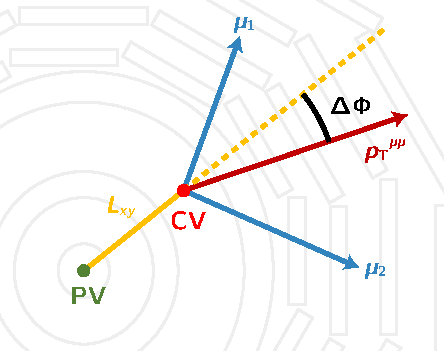
\includegraphics[width=.7\textwidth]{figures/displaced/LxyDef.pdf}
  \caption[Diagram of key variables (\Lxy and \DeltaPhi) used in the analysis.]{Diagram of the key variables used in this analysis. A long-lived particle is produced at the primary vertex (PV) and travels some distance in the detector before decaying into two muons ($\Pgm_1$ and $\Pgm_2$), forming a common vertex (CV). The distance between these two vertices in the transverse plane is referred to as \Lxy, the transverse decay length. The angle between the \Lxy vector and the \pT vector of the dimuon system is referred to as \DeltaPhi, the collinearity angle in the transverse plane.}
  \label{fig:dd:keyvars}
\end{figure}

The quantity \LxySig is referred as the \Lxy significance, as it is a measure of the significance of the fit compared to zero displacement.
For a well-reconstructed dimuon corresponding to a long-lived particle decaying a few tens of centimeters away from the PV, as in signal events, this quantity is large.
On the other hand, background events from reconstruction mistakes or promptly produced particles, such as can arise in Drell-Yan events, are expected to result in dimuons with small \Lxy significance.
A large \Lxy significance is therefore a strong indicator of consistency with the long-lived particle hypothesis.

The collinearity angle in the transverse plane between the dimuon \pT vector ($\pT^{\Pgm\Pgm}$) and the \Lxy vector is referred to as \DeltaPhi.
For a real pair of muons originating from a CV formed from the decay of a long-lived particle originating at the PV, the resulting dimuon momentum vector points towards the PV, and \DeltaPhi is small.
On the other hand, in most types of background events, this quantity is expected to be symmetric around $\pi/2$.
A small \DeltaPhi is therefore a strong indicator of consistency with the long-lived particle hypothesis.

We follow previous displaced dimuon searches \cite{EXO-12-037, CMS-PAS-EXO-14-012, ATLAS} in defining \Lxy as the unsigned magnitude of this distance.
The sign information regarding which side of the PV the CV is reconstructed is encoded in the companion variable \DeltaPhi, specifically in the sign of $\cos(\DeltaPhi)$.
(We call attention to this fact since other analyses in high-energy physics, for example $b$ physics analyses, typically attach the sign to \Lxy.)

\Fig~\ref{fig:dd:keyvars} illustrates these important quantities and their relationship to each other.

\section{Muon Reconstruction}
This analysis is a search for pairs of muons consistent with originating from a common vertex that is displaced with respect to the beam spot.
Such dimuon vertices can arise from decays of exotic long-lived particles, which are produced promptly (as a direct result of the hard interaction process and produced close to the beam spot) and travel for some distance before decaying.
As mentioned in \Sec~\ref{sec:dd:Trigger}, muons produced from such decays may not point towards the beam spot.
Most algorithms performing the offline reconstruction of muon tracks, however, include the beam spot; these reconstructions are described as being ``updated at the vertex.''
A search for displaced dimuons must therefore use a reconstruction algorithm that does not use this beam spot constraint.

Muons reconstructed using only hits in the muon system are known as standalone muons.
Standalone muon reconstruction is seeded with groups of segments in the muon system as a starting point for building a muon trajectory \cite{Liu2008}.
Standalone muons are independent of the more precise information from the silicon tracker, and so have poorer spatial and momentum resolution than muons reconstructed using the tracker.
However, the reconstruction efficiency for tracker tracks with transverse impact parameter $d_0$ (the closest distance between the track and the beam spot in the transverse plane) of more than a few tens of \cm is essentially zero, while the muon system gives non-vanishing reconstruction efficiency even a few meters away from the beam spot.
Therefore, standalone muons are the reconstructed object of choice for a displaced dimuon search sensitive to longer lifetimes.
Furthermore, standalone muon reconstruction is available with and without the beam spot constraint.
Standalone muons without this beam spot constraint are the starting point for choosing a muon reconstruction suitable for studying displaced dimuons.

The analyses performed using Run~1 data used refitted standalone muons (RSA muons) as their primary muon reconstruction \cite{CMS-PAS-EXO-14-012,CMS-AN-14-176}.
Compared to ordinary standalone muons without the beam spot constraint, the RSA muon algorithm computes a final refit (an additional iteration in the standalone muon trajectory builder) excluding the beam spot.
This reconstruction was intended to reduce the inherent bias towards the beam spot exhibited by the standard standalone muon reconstruction designed to study muons originating directly from the \pp collision.
RSA muons thus have improved $d_0$ and \pT resolution compared to standalone muons.

Another muon reconstruction algorithm is the displaced standalone muon (DSA muon) reconstruction.
Compared to ordinary standalone muons without the beam spot constraint, the DSA muon reconstruction is seeded with groups of segments in the muon chambers with criteria similar to those used for the reconstruction of cosmic muons (and thus more suitable for reconstruction of displaced muons), as opposed to seeds used for the reconstruction of muons originating from \pp collisions \cite{Liu2008, CMS-DP-2015-015}.
This reconstruction was intended to further improve the \pT resolution of muons produced from highly displaced decays.

\Fig~\ref{fig:dd:REFF} shows graphs of the efficiency as a function of generated \Lxy to reconstruct a generated muon as DSA or as RSA, with and without the trigger applied, with respect to \mbox{$\PHiggs\to2\PLLP\to2\Pgm$} signal events in which both generated muons are within a detector acceptance, defined as
\begin{itemize}
  \item both generated muon $\pT > 25\GeV$
  \item both generated muon $|\eta| < 2$
  \item generated \mbox{$\Lxy < 500\cm$}
\end{itemize}
In order to have a sufficient sample size, all 33 of the \twoMu signal samples are combined together for these graphs.
The reconstruction efficiency decreases steadily as a function of generated \Lxy, dropping off sharply at about 600\cm, corresponding roughly to the start of the third barrel muon station, and the DSA reconstruction is consistently higher than the RSA reconstruction.
With the trigger applied, the reconstruction efficiency is high for both DSA and RSA muons, up until about 300\cm at which point the trigger efficiency seriously limits the number of passing events.

\begin{figure}[p]
  \centering
  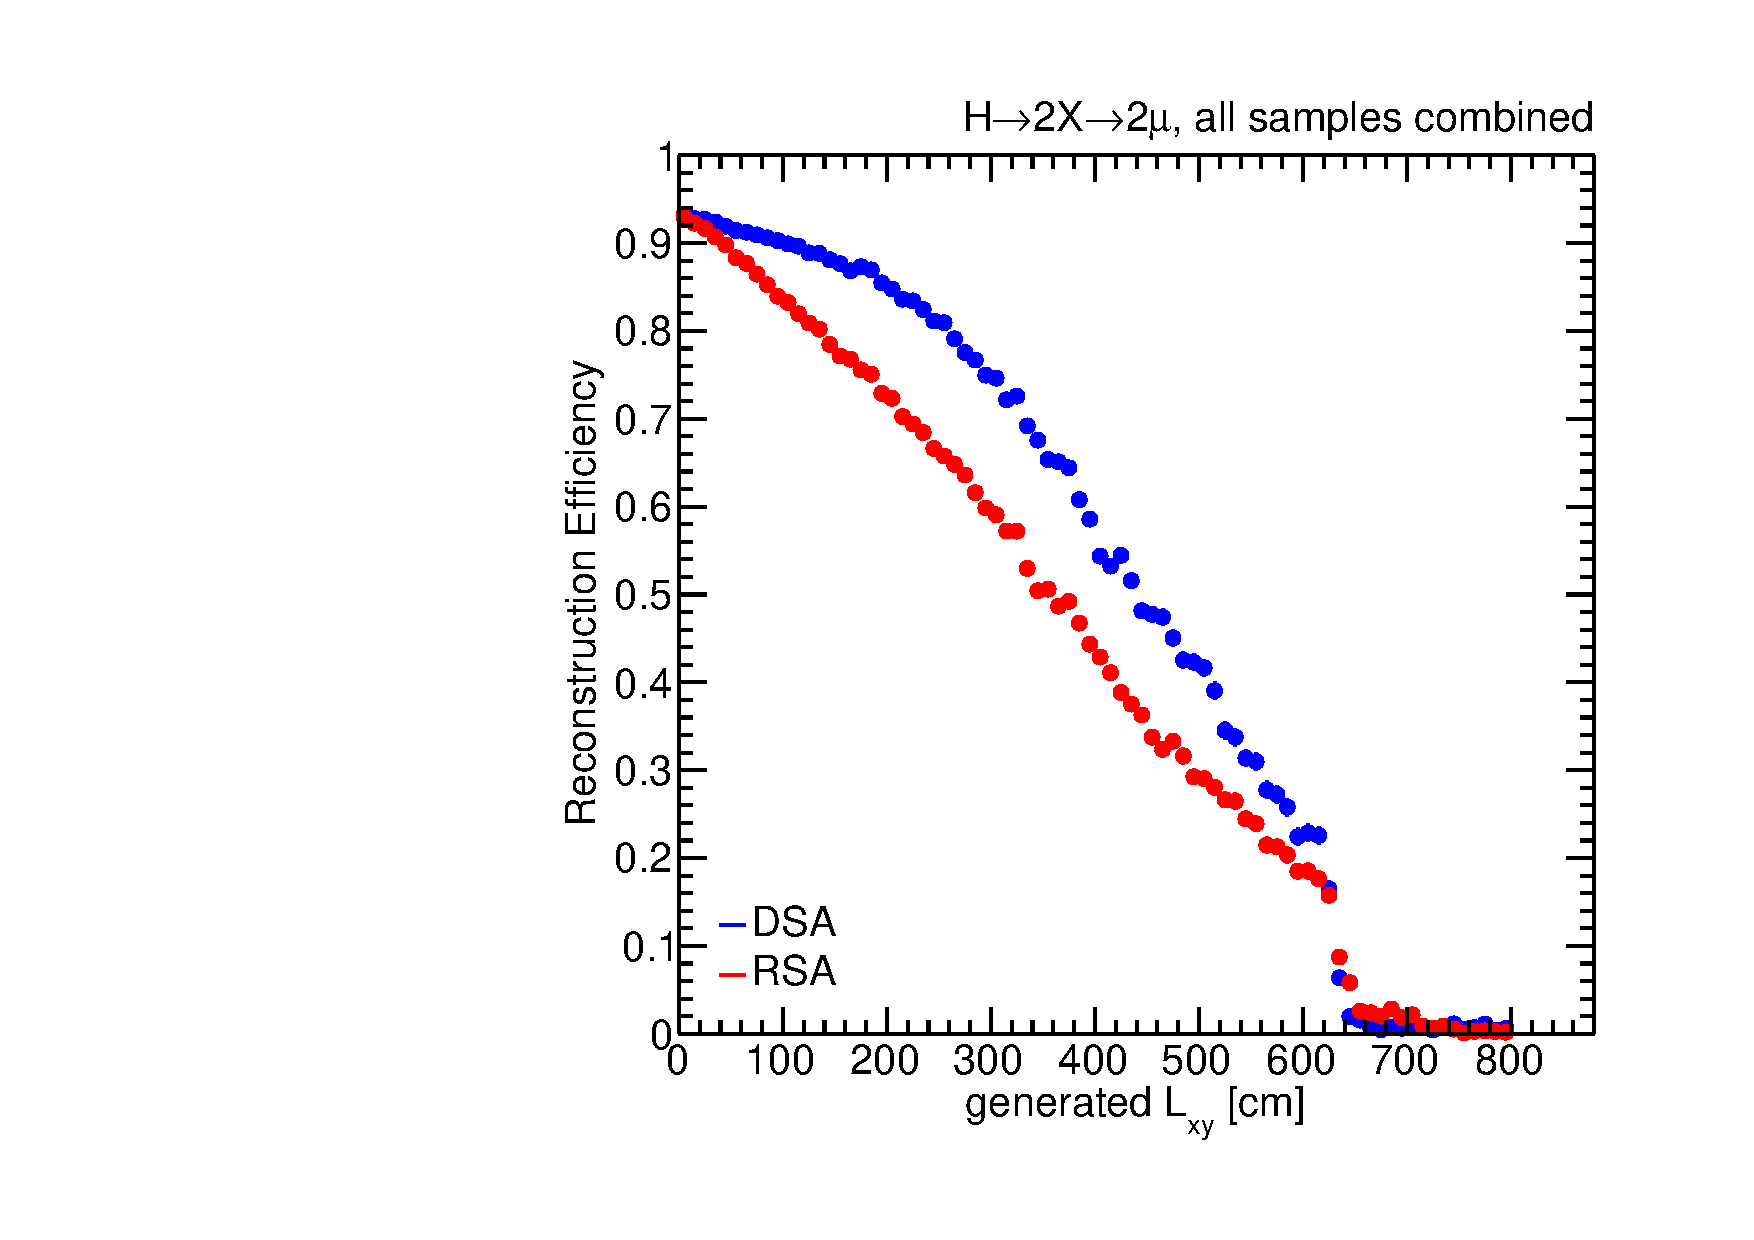
\includegraphics[width=\DSquareWidth]{figures/displaced/REFF_Lxy_2Mu2J_Global.pdf}
  \hspace*{-2em}
  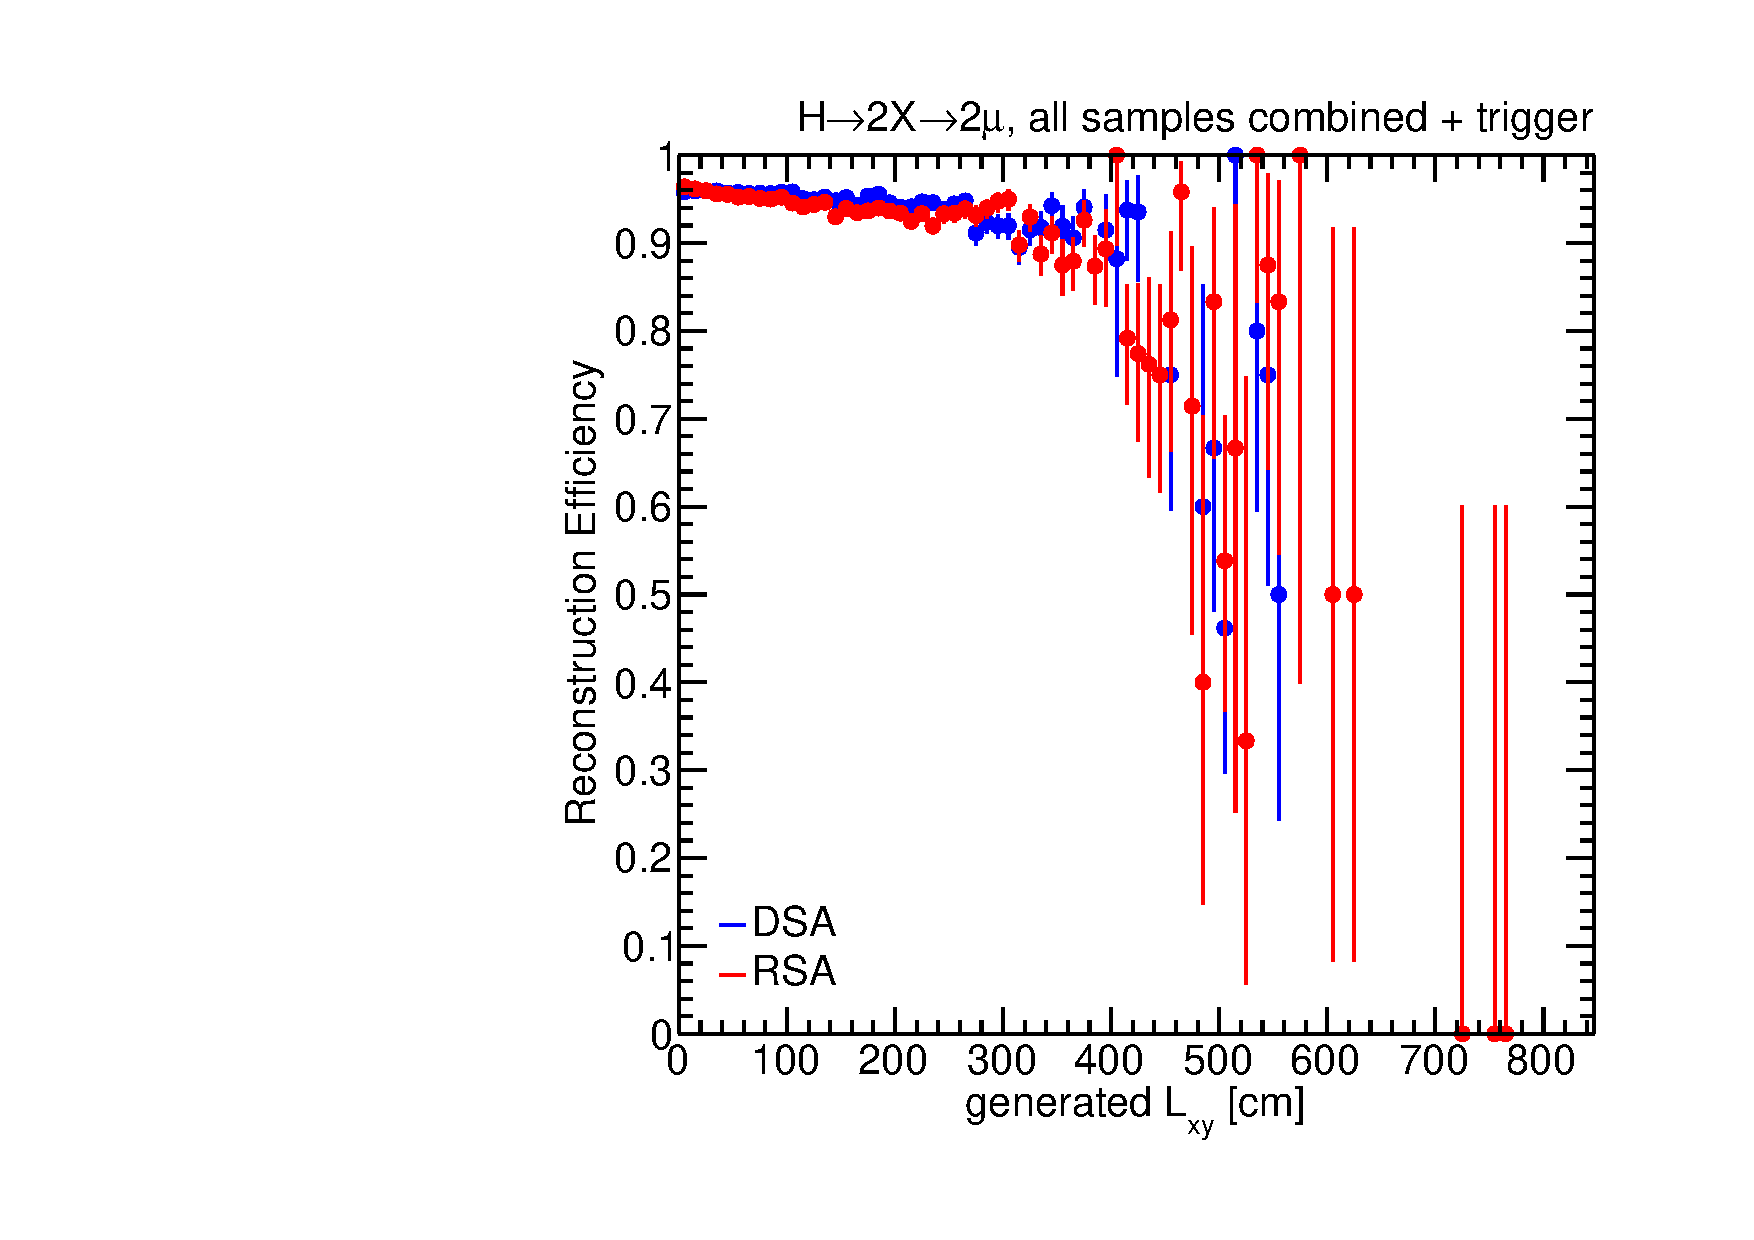
\includegraphics[width=\DSquareWidth]{figures/displaced/REFF_Lxy_Trig_2Mu2J_Global.pdf}
  \caption[DSA and RSA reconstruction efficiency as a function of generated \Lxy]{DSA and RSA reconstruction efficiency as a function of generated \Lxy for \twoMu signal events combining all 33 signal samples, with respect to events within acceptance, \figpos{left} without and \figpos{right} with the trigger applied. Error bars are for statistical uncertainty only.}
  \label{fig:dd:REFF}
\end{figure}
\begin{figure}[p]
  \centering
  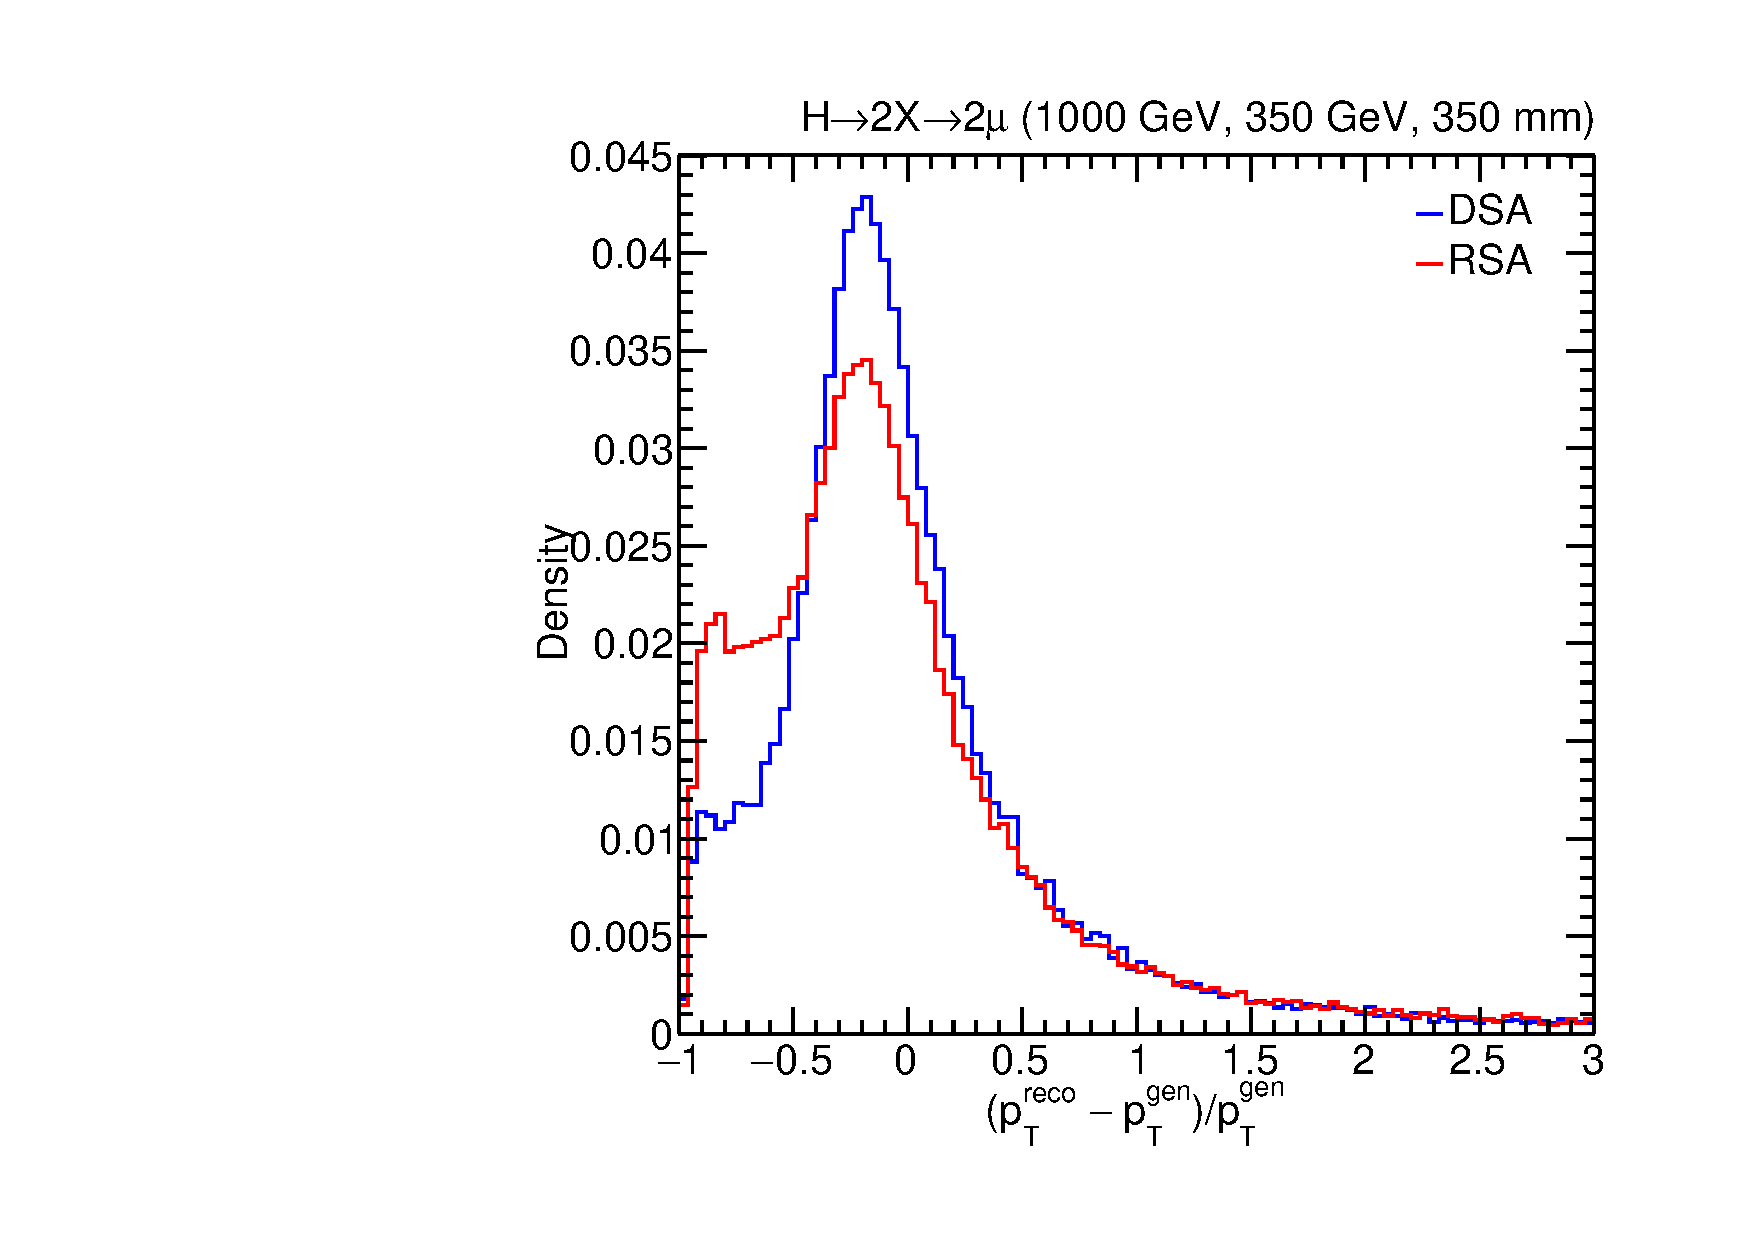
\includegraphics[width=\DSquareWidth]{figures/displaced/PTRES_2Mu2J_1000_350_350.pdf}
  \hspace*{-2em}
  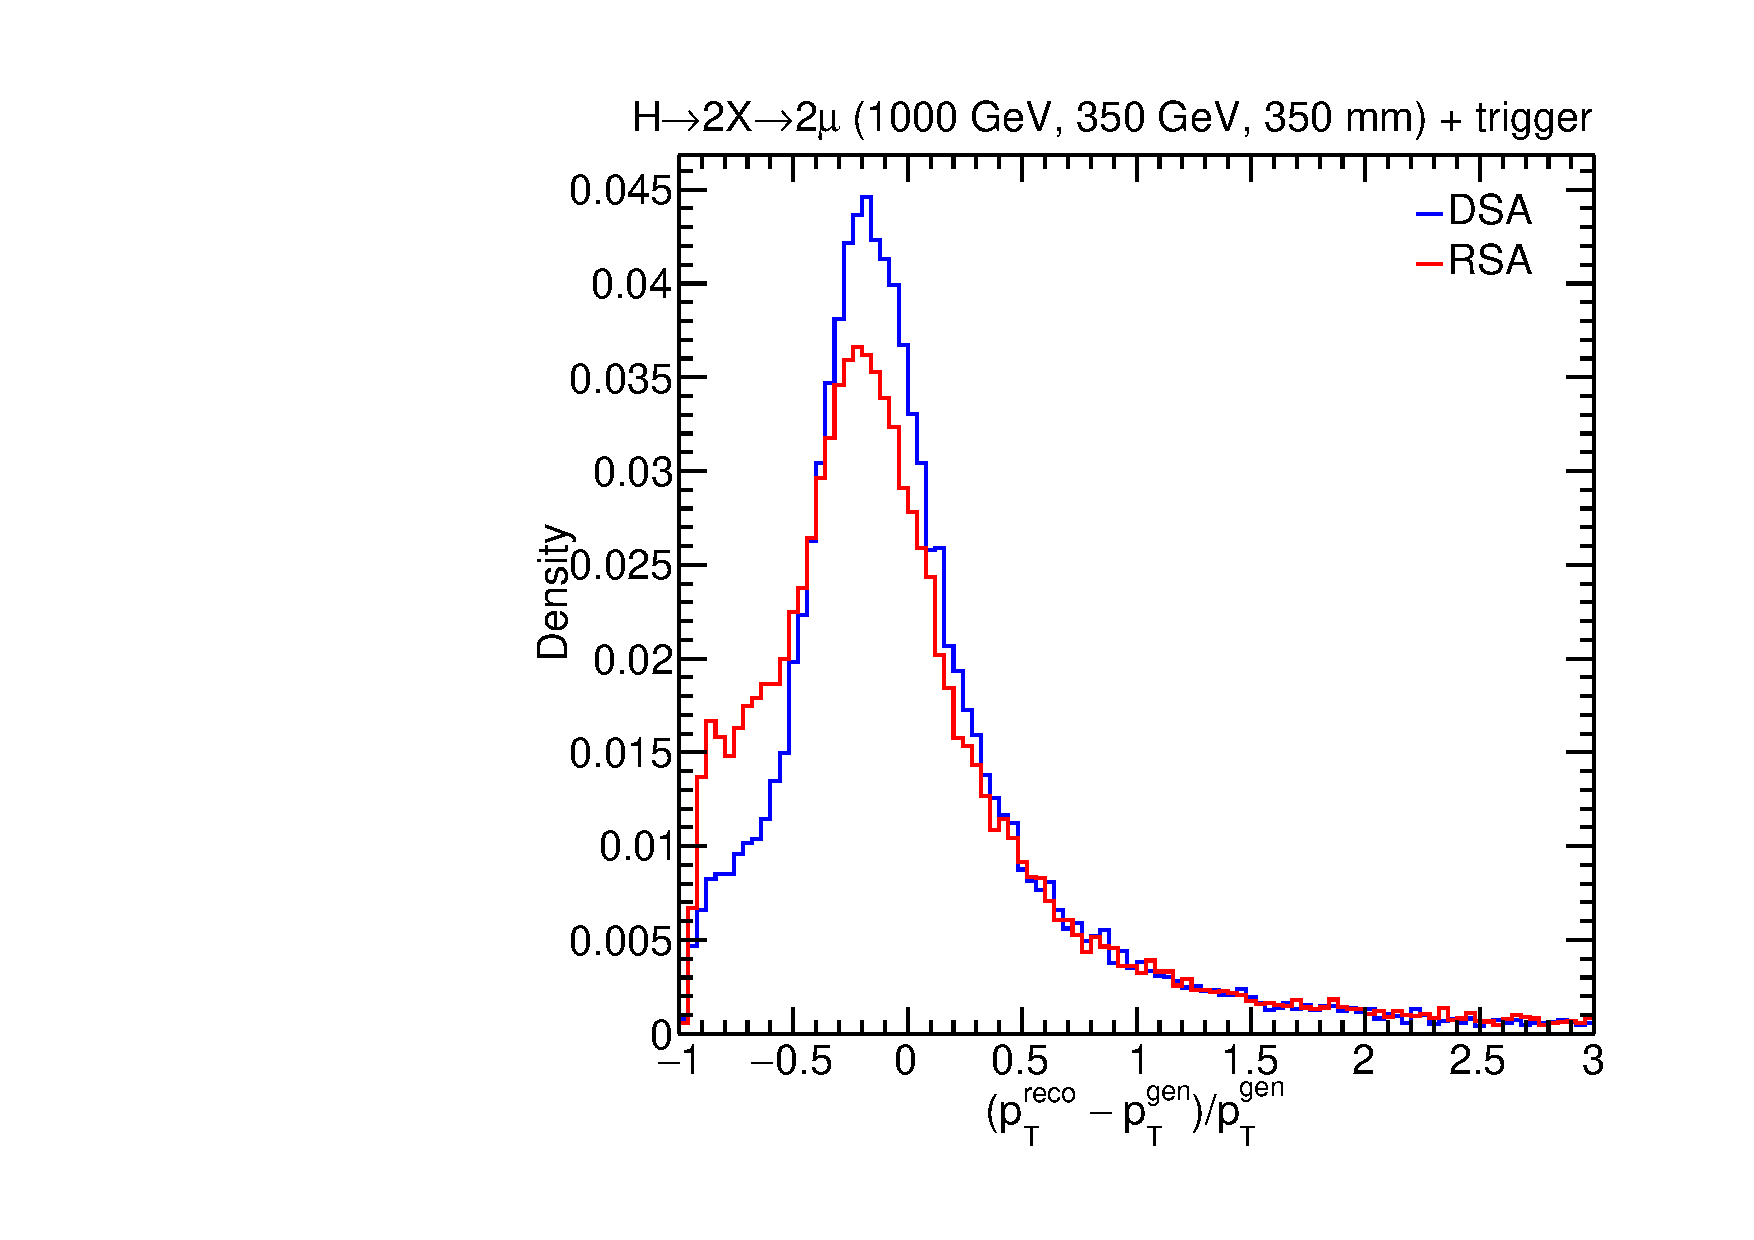
\includegraphics[width=\DSquareWidth]{figures/displaced/PTRES_Trig_2Mu2J_1000_350_350.pdf}
  \caption[DSA and RSA \pT resolution for generated events within acceptance]{DSA and RSA \pT resolution for generated events within acceptance, \figpos{left} without the trigger applied and \figpos{right} with the trigger applied, for the \twoMu signal sample with \FullSP{1000}{350}{350}.}
  \label{fig:dd:PTRES_DSA_RSA}
\end{figure}


\Fig~\ref{fig:dd:PTRES_DSA_RSA} shows distributions of the \pT resolution for the DSA and RSA reconstructions, normalized to unit area, for generated events within acceptance, with and without the trigger applied, for the \twoMu signal sample with \FullSP{1000}{350}{350}.
The RSA reconstruction gives a visibly worse \pT resolution, with a larger shoulder near $-1$, indicating that RSA muons tend to underestimate the muon \pT compared to DSA muons.

\Figs~\ref{fig:dd:REFF}--\ref{fig:dd:PTRES_DSA_RSA} show that DSA muons have both a higher reconstruction efficiency and an improved \pT resolution over RSA muons.
The analysis presented in this thesis therefore primarily uses DSA muons.

\section{Event and Object Selection}
\subsection{Overview}
\label{sec:dd:GeneralStrategy}
This section presents details of the selection criteria used to perform the analysis.
Informally, selection criteria are referred to as cuts, as application of selection criteria cuts away events.
An overview of the general strategy for selecting reconstructed events and objects consistent with displaced dimuons is as follows.
\clearpage
\begin{enumerate}
  \item \textbf{DSA muon preselection}. Begin with DSA muons as seeds for searching for displaced dimuons and apply a set of quality criteria to select muons that are reasonably well reconstructed. (\Sec~\ref{sec:dd:DSAQuality})
  \item \textbf{HLT-RECO matching}. Keep only events that contain offline reconstructed muons that match the online trigger muons passing the HLT. (\Sec~\ref{sec:dd:HLTMatching})
  \item \textbf{\DSAToPAT muon association}. Attempt to associate DSA muons with global or arbitrated tracker muons (referred to as PAT muons, named after the \textbf{P}hysics \textbf{A}nalysis \textbf{T}ools in the CMS software that process them), and if they can be, replace the DSA muons with the associated PAT muons. This analysis focuses on the DSA muons that are \emph{not} associated with PAT muons, so this step essentially sets aside DSA muons that are consistent with muons reconstructed using the tracker. (\Sec~\ref{sec:dd:Association})
  \item \textbf{DSA muon object selection}. Apply additional selections to remaining DSA muons that identify DSA muons in signal-like events and ensure that they are of good quality. (\Sec~\ref{sec:dd:DSAObject})
  \item \textbf{Dimuon formation from common vertex fit}. Form dimuons by fitting two DSA muon tracks to a common vertex. (\Sec~\ref{sec:dd:DimVertex})
  \item \textbf{Pairing criteria}. Select the 1--2 dimuons most likely to be signal dimuons according to a set of muon pairing criteria. (\Sec~\ref{sec:dd:PC})
  \item \textbf{Dimuon object selection}. Apply additional selections to dimuons that identify dimuons in signal-like events and ensure they are of good quality. (\Sec~\ref{sec:dd:DimuonObject})
  \item \textbf{Dimuon signal selection}. Apply additional selections to dimuons that require the dimuon be displaced from the beam spot and have a form consistent with the signal hypothesis that the dimuon originates from the decay of a long-lived particle into two oppositely-charged muons. (\Sec~\ref{sec:dd:DimuonSignal})
  \item \textbf{Cosmic muon suppression}. Apply additional requirements to suppress background events from cosmic muons. (\Sec~\ref{sec:dd:CosmicCuts})
\end{enumerate}

\subsection{DSA Muon Preselection}
\label{sec:dd:DSAQuality}
Event and object preselection begins with DSA muons.
The HLT path described in \Sec~\ref{sec:dd:Trigger} reconstructs muons at Level~2 using a procedure similar to that used to reconstruct muons as refitted standalone (RSA) muons at the offline reconstructed level.
However, as discussed in the previous section, DSA muons are chosen as the starting point over RSA muons for their improved \pT resolution and higher reconstruction efficiency.
DSA muons are required to satisfy the following quality criteria:
\begin{itemize}
  \item reconstructed with hits in at least two muon stations, \ie $$N(\text{CSC stations}) + N(\text{DT stations}) > 1$$
  \item reconstructed with at least 13 hits in the muon stations, \ie $$N(\text{CSC hits}) + N(\text{DT hits}) > 12$$
  \item relative \pT uncertainty of less than 100\%, \ie $$\pTErr/\pT < 1$$
\end{itemize}

These quality criteria ensure that the DSA muons have acceptable \pT resolution and charge assignment.
\Fig~\ref{fig:dd:QCUT_PTRES} shows distributions of the DSA muon \pT resolution for the \twoMu signal sample with \FullSP{1000}{350}{350} for events split up by the $N_\text{hits}$ cut and for events split up by the $\pTErr/\pT$ cut, each population normalized to unit area.
The events satisfying the cut have reasonable \pT resolution, while the events failing the cut have rather poor \pT resolution.
\Fig~\ref{fig:dd:QCUT_QDIFF} shows distributions of the difference between reconstructed and generated charge for the same signal sample, for events split up by the $N_\text{hits}$ cut and for events split up by the $\pTErr/\pT$ cut, each population normalized to unit area.
The events satisfying the cut are assigned the correct charge in more than 90\% of events, while the events failing the cut are assigned the correct charge in only around 60\% of events.

\begin{figure}[htpb]
  \centering
  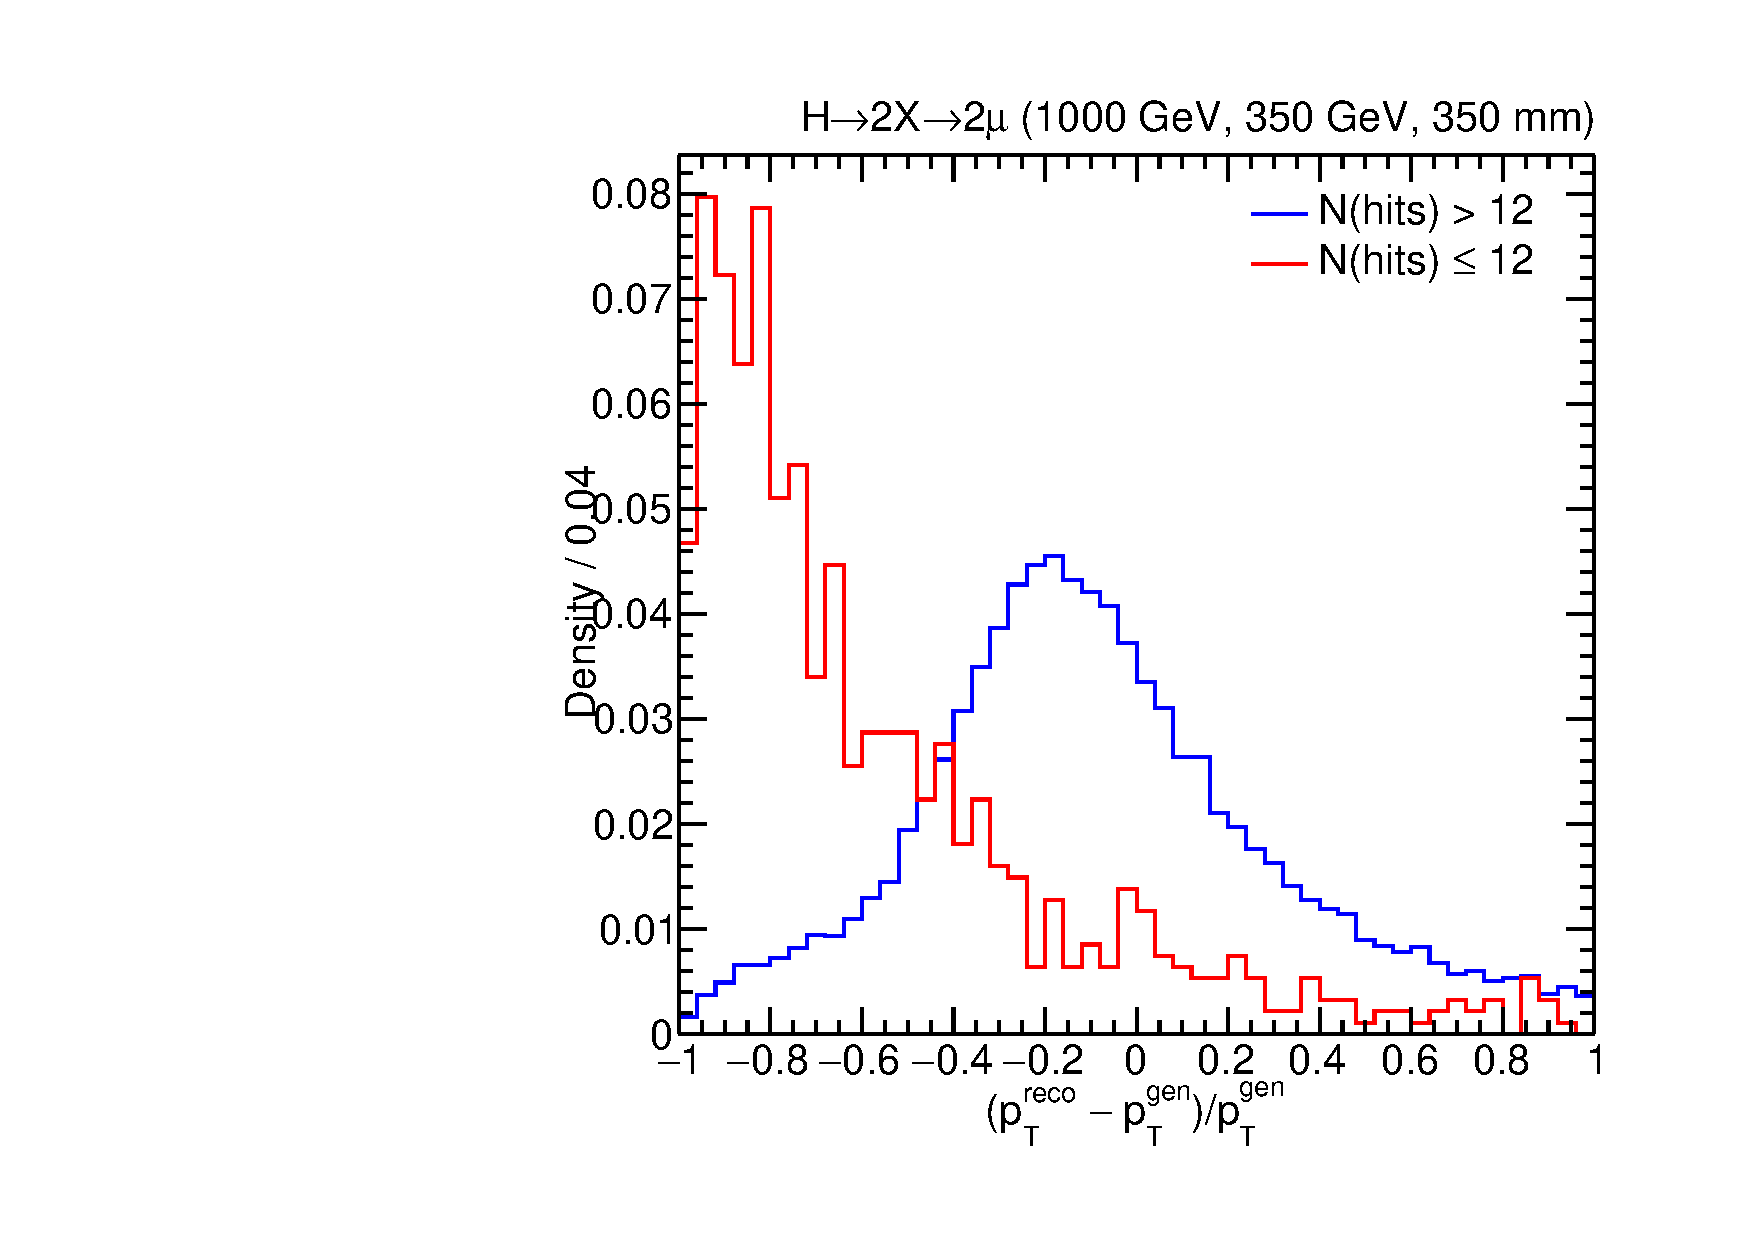
\includegraphics[width=\DSquareWidth]{figures/displaced/QCUTRES_Sig_pTRes_hits_1000_350_350.pdf}
  \hspace*{-2em}
  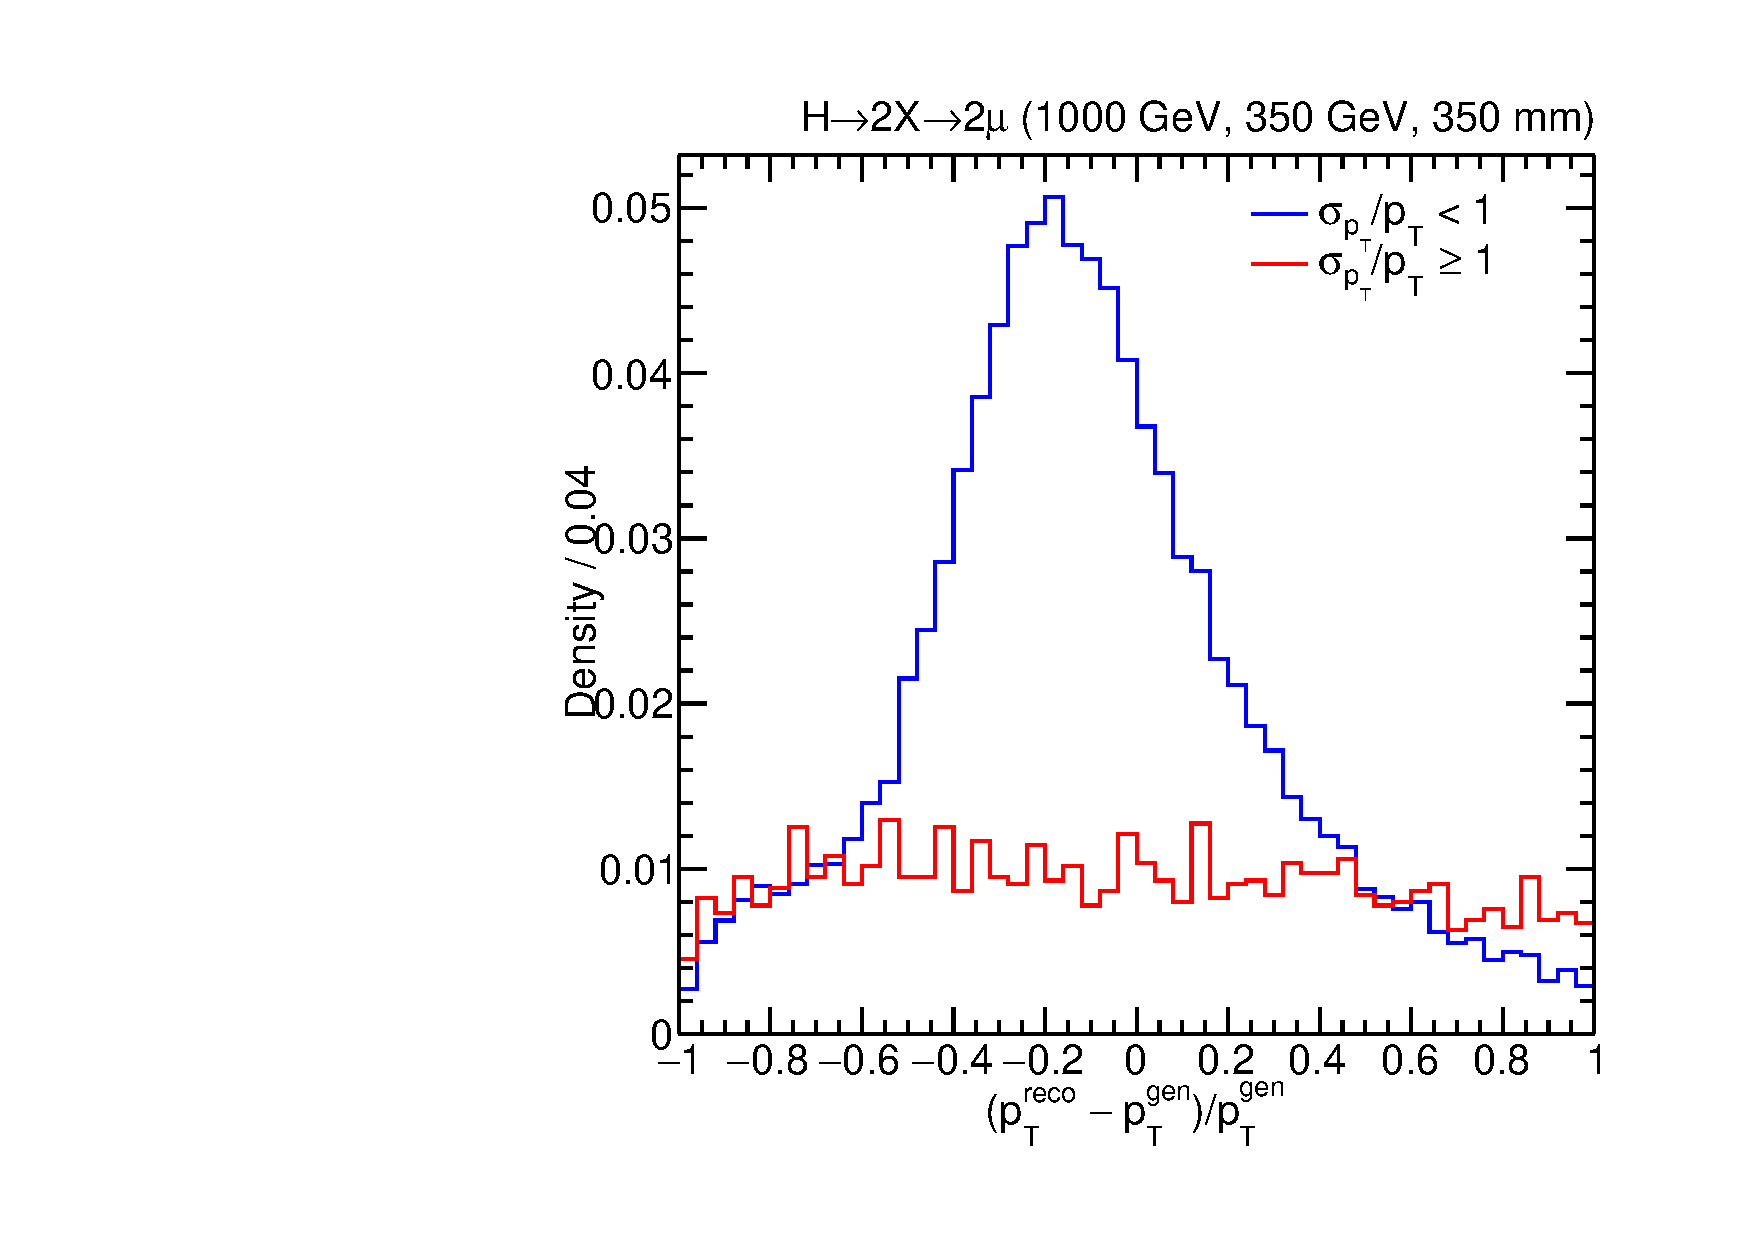
\includegraphics[width=\DSquareWidth]{figures/displaced/QCUTRES_Sig_pTRes_fpte_1000_350_350.pdf}
  \caption[DSA muon \pT resolution with and without selections on $N_\text{hits}$ and $\pTErr/\pT$.]{DSA muon \pT resolution, normalized to unit area, for the \twoMu signal sample with \FullSP{1000}{350}{350} for \figpos{left} events with $N_\text{hits} > 12$ and $N_\text{hits} \leq 12$ separately, and \figpos{right} events with $\pTErr/\pT \geq 1$ and $\pTErr/\pT < 1$ separately.}
  \label{fig:dd:QCUT_PTRES}
\end{figure}
\begin{figure}[htpb]
  \centering
  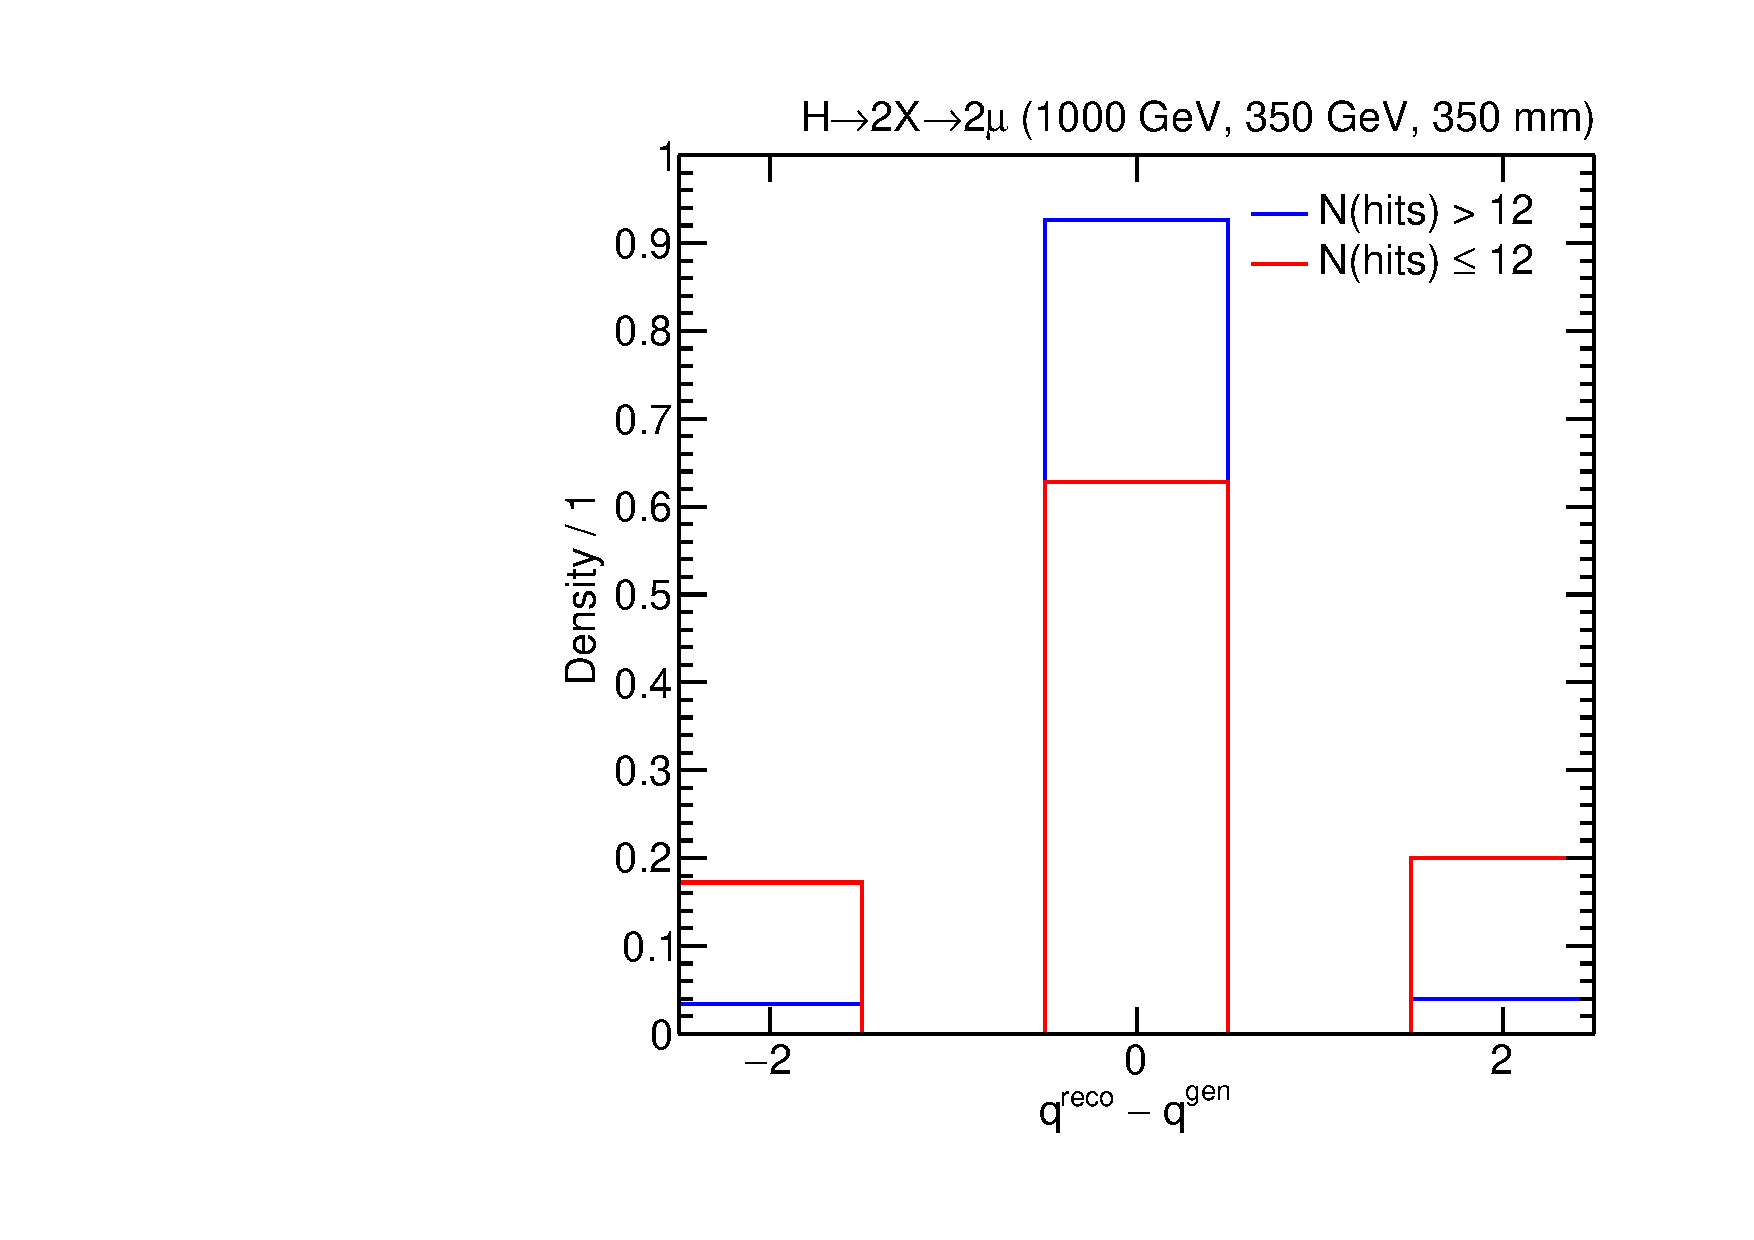
\includegraphics[width=\DSquareWidth]{figures/displaced/QCUTRES_Sig_qdiff_hits_1000_350_350.pdf}
  \hspace*{-2em}
  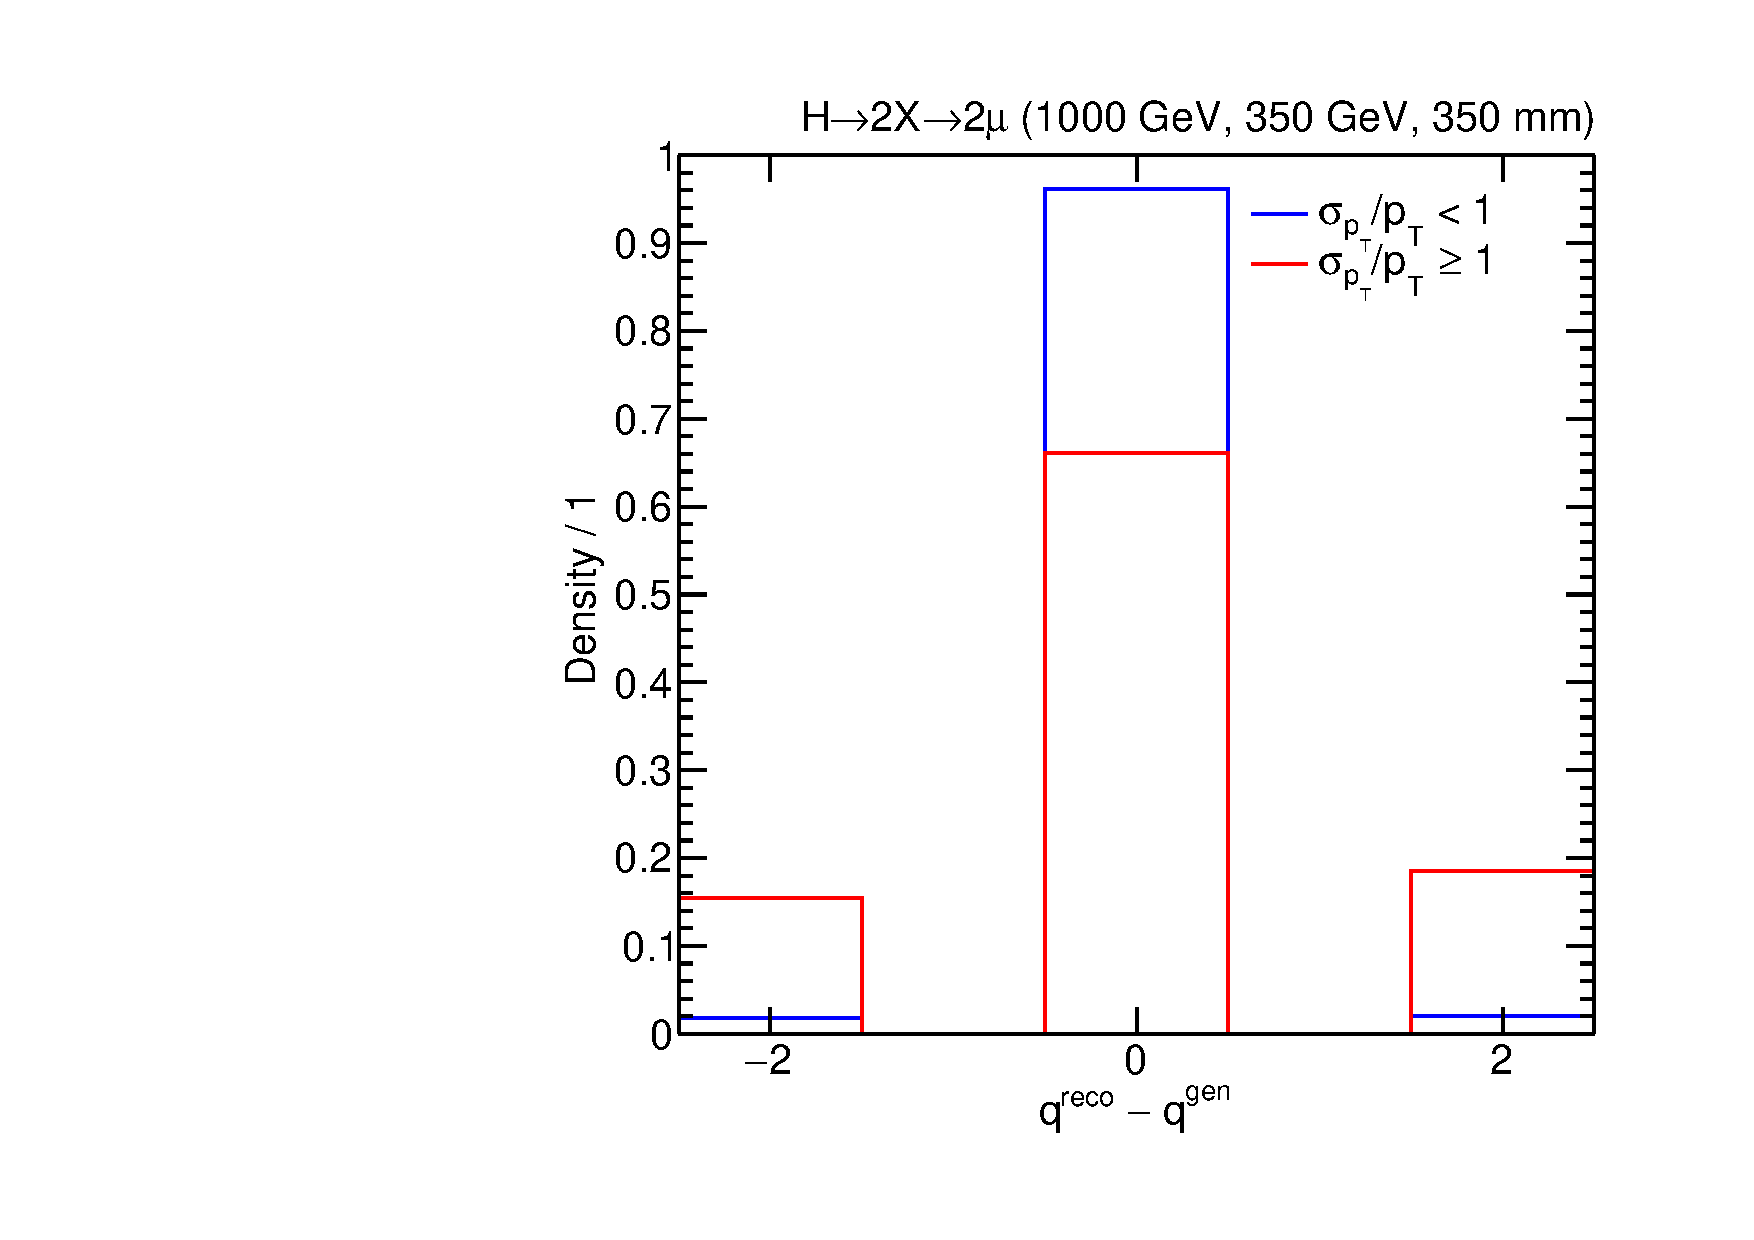
\includegraphics[width=\DSquareWidth]{figures/displaced/QCUTRES_Sig_qdiff_fpte_1000_350_350.pdf}
  \caption[DSA muon charge difference with and without selections on $N_\text{hits}$ and $\pTErr/\pT$.]{DSA muon charge difference, normalized to unit area, for the \twoMu signal sample with \FullSP{1000}{350}{350} for \figpos{left} events with $N_\text{hits} > 12$ and $N_\text{hits} \leq 12$ separately, and \figpos{right} events with $\pTErr/\pT \geq 1$ and $\pTErr/\pT < 1$ separately.}
  \label{fig:dd:QCUT_QDIFF}
\end{figure}

\subsection{HLT-RECO Matching}
\label{sec:dd:HLTMatching}
Next, only events in which the HLT decision is matched using the preselected DSA muons are kept, in a procedure referred to as HLT-RECO matching.
This ensures that the quickly-reconstructed, coarser-resolution muons reconstructed by the trigger system have counterparts among muons reconstructed offline using the higher-precision data of the full event.
For the purposes of HLT-RECO matching, DSA muons are required to pass loose \pT and $\eta$ requirements: $\pT > 10\GeV$ and $|\eta| < 2.0$.
These DSA muons are referred to as DSA muons for trigger matching.
Let \deltaR refer to the angular proximity in $\eta$-$\phi$ space between two three-vectors, defined as
\begin{equation}
  \Delta R = \sqrt{\left(\Delta\eta\right)^2 + \left(\Delta\phi\right)^2}
  \label{eq:dd:deltaR}
\end{equation}
Then HLT-RECO matching requires that each of the pair of distinct DSA muons for trigger matching lie within cones of $\deltaR < 0.4$ around each muon among pairs of muons reconstructed at Level~2 passing the trigger (HLT muons).

The \pT, $\eta$, and \deltaR requirements are all chosen to empirically optimize the trade-off between efficiency and purity, matching as many events as possible while keeping the frequency of accidental matches to poor quality muons low.
The HLT-RECO matching procedure retains more than 98\% of \twoMu signal events that passed the trigger and have at least two DSA muons for trigger matching.

The HLT-RECO matching requirement ensures, at the event level, that the trigger decision is confirmed using objects reconstructed offline.
The subsequent object selection, however, does not require that selected dimuons be formed from pairs of triggering HLT muons.
This allows the analysis to be sensitive to \fourMu final states, in which two of the four muons passed the trigger, but all four muons are signal muons.

\subsection{\DSAToPAT Muon Association}
\label{sec:dd:Association}
This analysis begins with DSA muons to identify potential displaced muon events, specifically focusing on highly displaced events in which the long-lived particle travels far enough before decaying that a track is not observed in the tracker.
Implementing this requirement necessitates development of a procedure to efficiently associate DSA muons with muons reconstructed using the tracker.
This association improves not only potential signal discrimination, but also background rejection.
Ensuring that this procedure is both highly efficient (\ie muons that should be associated, are) and highly pure (\ie muons that should not be associated, are not) requires some care.
This section describes the details of the association procedure.

\subsubsection{PAT Muons and Matching Criteria}
Offline reconstructed muons having either of the following properties are considered:
\begin{itemize}
  \item \textbf{Global muons}. Global muons are muons reconstructed by association a tracker track with a standalone muon by collecting all the hits from both and performing a full track fit, called a global muon fit. Global muons are the primary muon reconstruction used by most CMS analyses.
  \item \textbf{Arbitrated tracker muons}. In order to deal with cases in which global muon reconstruction is inefficient, tracker muons were developed. Tracker muons do not require a standalone muon; instead, a tracker track is extrapolated and associated with hits in the muon system. In the case of multiple tracker tracks associated with the same muon hits, an algorithm called arbitration chooses which association to prefer such that no two tracker muons share muon segments; these tracker muons are referred to as arbitrated tracker muons.
\end{itemize}
The muons considered in this analysis that are reconstructed offline using both the tracker and the muon system are referred to as PAT muons.
(PAT is an abbreviation for \textbf{P}hysics \textbf{A}nalysis \textbf{T}ools, a toolkit that is part of the CMS software and which is used to process event and object reconstruction.)
A PAT muon may be both a global muon and an arbitrated tracker muon, and good quality PAT muons are often both.

Candidate PAT muons are associated with DSA muons when they satisfy one of two matching criteria, which are applied in different contexts in a procedure described below. The two matching criteria are:
\begin{itemize}
  \item \textbf{Segment-matched}: A PAT muon is segment-matched to a DSA muon if the PAT muon shares all of its muon system segments with at least 2/3 of the muon system segments used to reconstruct the DSA muon. PAT muon segments and DSA muon segments are compared coordinate by coordinate for equality and are considered the same if their coordinates match.
  \item \textbf{Proximity-matched}: A PAT muon is proximity-matched to a DSA muon if the \deltaR between
    \begin{itemize}
      \item the position vector of the innermost hit of the DSA muon and
      \item the position vector of the point of closest approach of the PAT muon helically extrapolated (in the magnetic field) to the innermost hit of the DSA muon.
    \end{itemize}
    is less than 0.4, with tighter requirements applied in the procedure described below.
\end{itemize}

The proximity match is defined as it is above because DSA muons are sometimes reconstructed with an incorrect $\eta$ coordinate, and would not pass a more standard angular proximity match between the momentum directions of the DSA and PAT muons.
The helical extrapolation and comparison between the positions improved the efficiency of the proximity match.

\subsubsection{\DSAToPAT Association Procedure}
The general procedure is as follows: given a DSA muon, associate segment-matched PAT muons with the DSA muon, using additional criteria to disambiguate among multiple segment-matched PAT muons.
These additional disambiguation criteria include requiring that segment-matched PAT muons are also the PAT muon with the smallest proximity-match \deltaR (as defined above) and/or requiring that segment-matched muons be global and that they be reconstructed from hits in at least 7 tracker layers.
If no PAT muons segment-match the DSA muon, the smallest-\deltaR proximity-matched PAT muon is associated with the DSA muon if its proximity-match \deltaR is sufficiently small; the threshold is 0.4 if the proximity-matched PAT muon is global and has the same numbers of muon system hits as the DSA muon, and 0.1 otherwise.
The full technical details of the procedure are depicted in \Fig~\ref{fig:dd:repdiagram}.

\begin{figure}[p]
  \centering
  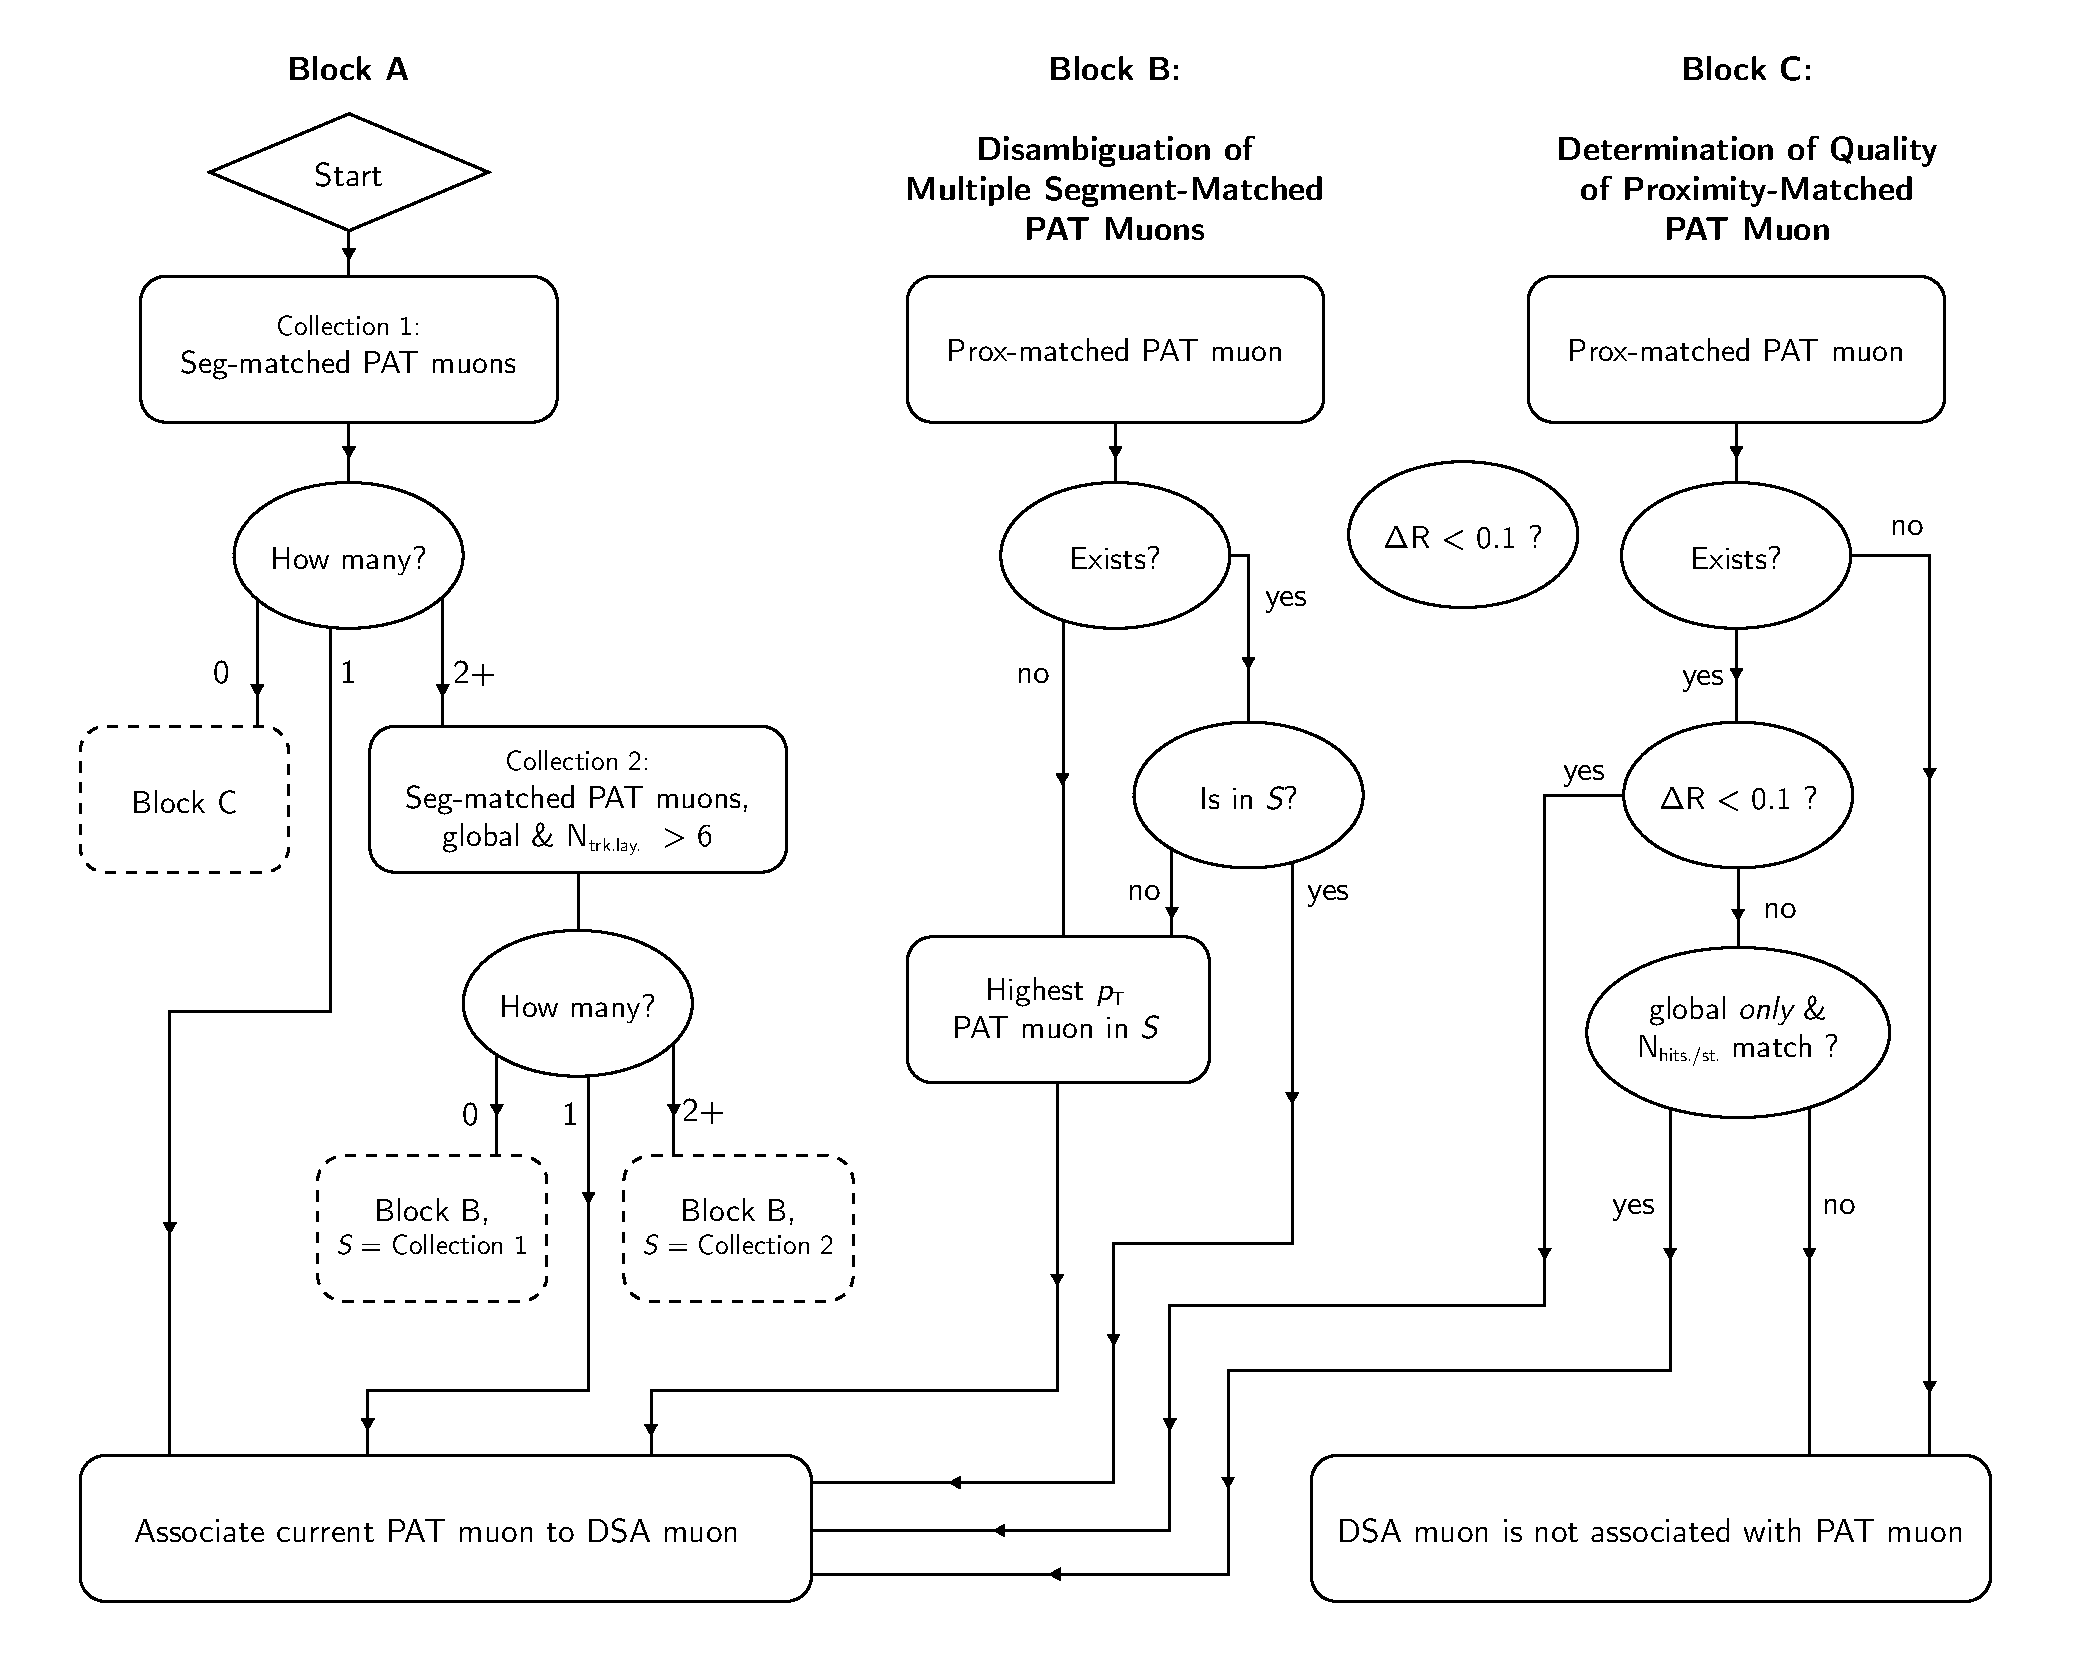
\includegraphics[width=\textwidth]{figures/displaced/ReplacementDiagram.pdf}
  \caption[Flowchart depicting the technical details of the \DSAToPAT association procedure]{Flowchart depicting the technical details of the \DSAToPAT association procedure. The procedure begins by considering segment-matched PAT muons. If there are multiple segment-matched PAT muons, then some temporary quality cuts are applied: the requirements that the muon be global and that it be reconstructed from at least 7 tracker layers (abbreviated $N_\text{trk. lay.}$). When there are multiple segment matches, the PAT muon that has the smallest proximity-match \deltaR is used to disambiguate between them, if possible. If there are no segment matches, then the proximity-matched PAT muon is taken as the match if its proximity \deltaR is sufficiently small. This threshold is 0.4 if the PAT muon is global only (not tracker) and its numbers of CSC and DT hits and stations (abbreviated $N_\text{hits./st.}$) matches those of the DSA muon exactly, and 0.1 otherwise.}
  \label{fig:dd:repdiagram}
\end{figure}

This procedure prioritizes segment-matched PAT muons over proximity-matched PAT muons.
Several combinations of criteria are used to determine the quality selection used to disambiguate segment-matched PAT muons; the combination used here (global and number of tracker layers) is found to be optimal in terms of increasing the efficiency to match to the correct PAT muon.
In principle, there exists the case that a proximity-matched PAT muon does not exist or is not among the segment-matched PAT muons.
In this case, we were prepared to fall back to associating to the highest-\pT PAT muon among the collection of segment-matched PAT muons.
However, this situation never actually occurs in practice.

The \deltaR threshold in the case that there are no segment-matched PAT muons is chosen empirically to increase the matching efficiency while keeping the rate of false, accidental matches low.
At the time of this writing, this analysis does not access the muon system segments used to reconstruct the standalone muons used to form global muons, and so a PAT muon that is global only cannot be segment-matched to a DSA muon.
This has little practical effect on the efficiency to correctly associate DSA muons with PAT muons in this analysis.
For the small fraction of PAT muons that are global only and should be associated with a DSA muon, the proximity-matched PAT muon is often the correct choice.
Therefore, the \deltaR threshold for proximity-matched global-only PAT muons is set at 0.4, if their numbers of CSC and DT hits and stations are identical to those of the DSA muon.
As missed matches can lead to a high rate of background events which are potentially dangerous, this association procedure is also designed to be liberal in order to reject background events: if a DSA muon can be reasonably associated with a PAT muon, it should be, even at the cost of a few accidental matches.
Therefore, in the case of no segment-matched PAT muons and a proximity-matched PAT muon that is a tracker muon, the procedure associates with the DSA muon the proximity-matched PAT muon if its proximity \deltaR is less than 0.1 as a final compromise between efficiency and purity.

As mentioned in \Sec~\ref{sec:dd:mcsamples}, the analysis presented in this thesis focuses only on the DSA muons that are not associated with PAT muons.
To this end, DSA muons are replaced with any associated PAT muons, and so the association step effectively functions as a rejection of DSA muons that can be associated with PAT muons.
The effect of this is that this analysis, using DSA muons, does not benefit from the improved resolution of PAT muons, but it benefits tremendously from the superior background rejection.
This is the analysis sensitive to the longest lifetimes, with long-lived particles decaying in the outer region of the tracker and outside the tracker through the muon system.

The PAT association procedure is highly effective in suppressing \pp collision backgrounds, such as those modeled by the simulated background samples.
\Figs~\ref{fig:dd:REPEFF_MC_LxySig}--\ref{fig:dd:REPEFF_MC_Lxy} are histograms of dimuon \LxySig and \Lxy in simulated background samples, with each process scaled to its equivalent luminosity as discussed in \Sec~\ref{sec:dd:EqLumi}, before and after the association procedure.
The PAT association suppresses events in simulated background by a factor of $10^5$, reducing the number of dimuons from 12.5 million to 204.
For these histograms, a \pT cut of 10\GeV is applied to DSA muons on top of the preselection criteria.
This is a requirement that is part of the muon object selection (see \Sec~\ref{sec:dd:DSAObject}), but is applied here to more clearly demonstrate the effect of the PAT association procedure by suppressing secondary, low-\pT muons not associated with PAT muons, such as those from other \pp collisions in the bunch crossing.

\begin{figure}[p]
  \centering
  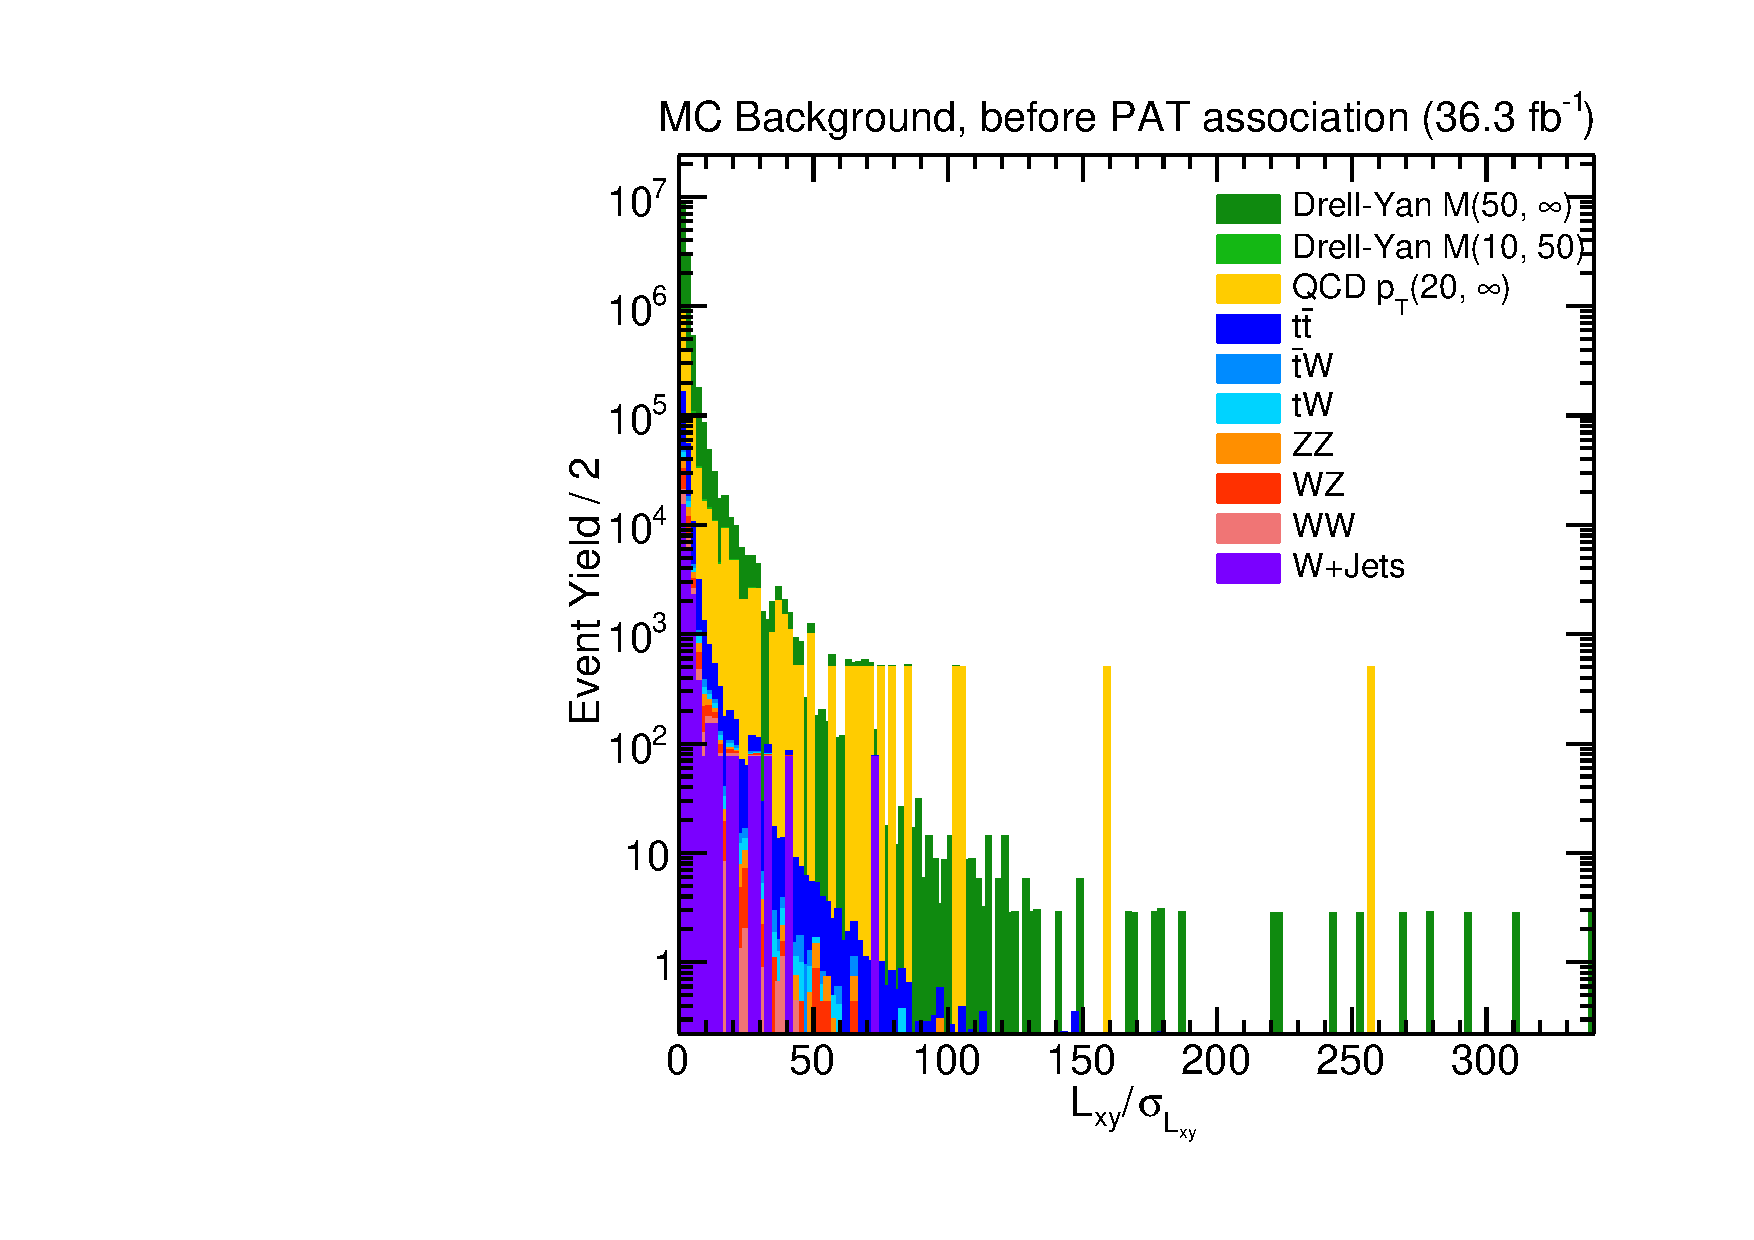
\includegraphics[width=\DSquareWidth]{figures/displaced/REPEFF_MC_LxySig-before.pdf}
  \hspace*{-2em}
  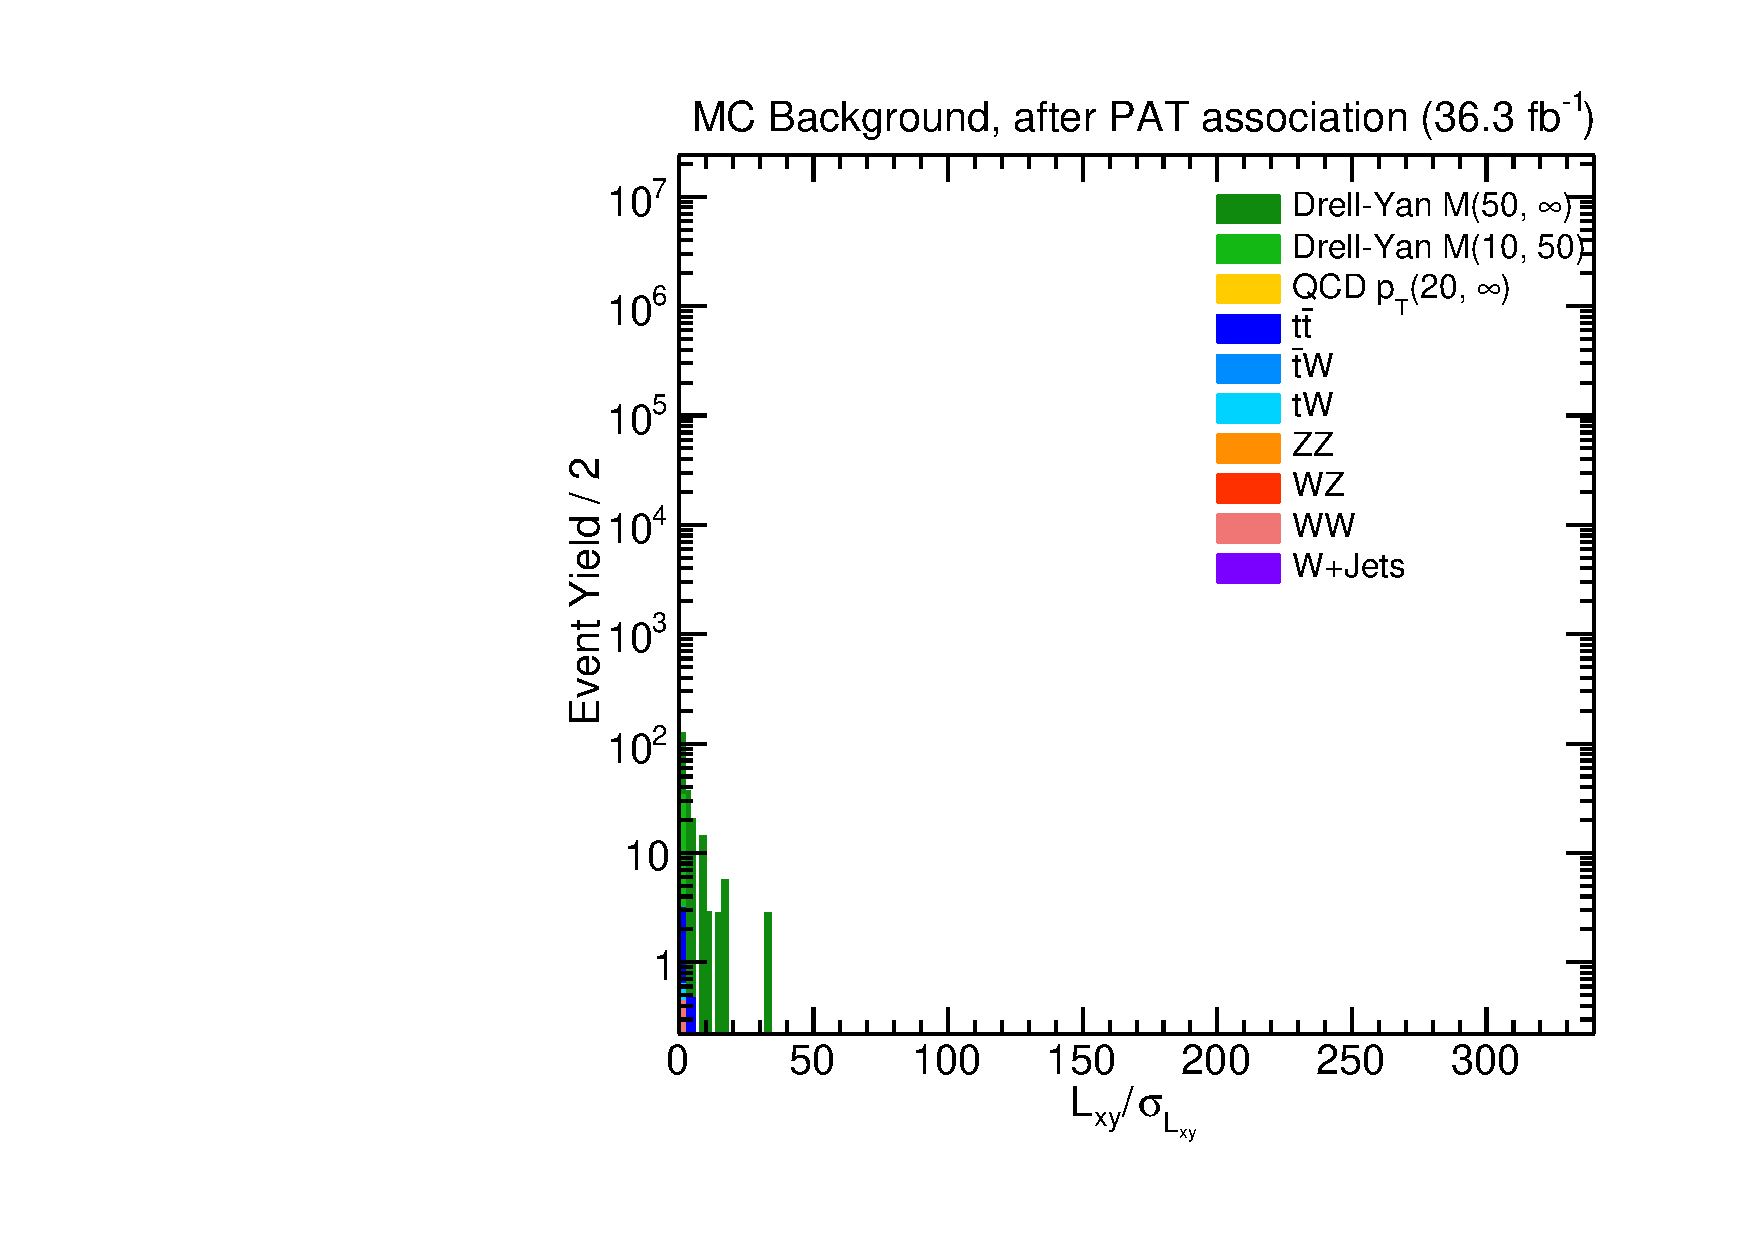
\includegraphics[width=\DSquareWidth]{figures/displaced/REPEFF_MC_LxySig-after.pdf}
  \caption[Histogram of dimuon \LxySig in simulated background samples before and after the PAT association procedure.]{Histogram of dimuon \LxySig in simulated background samples, scaled to 2016 integrated luminosity, \figpos{left} before and \figpos{right} after the PAT association procedure. The procedure suppresses the number of background events by a factor of $10^5$.}
  \label{fig:dd:REPEFF_MC_LxySig}
\end{figure}
\begin{figure}[p]
  \centering
  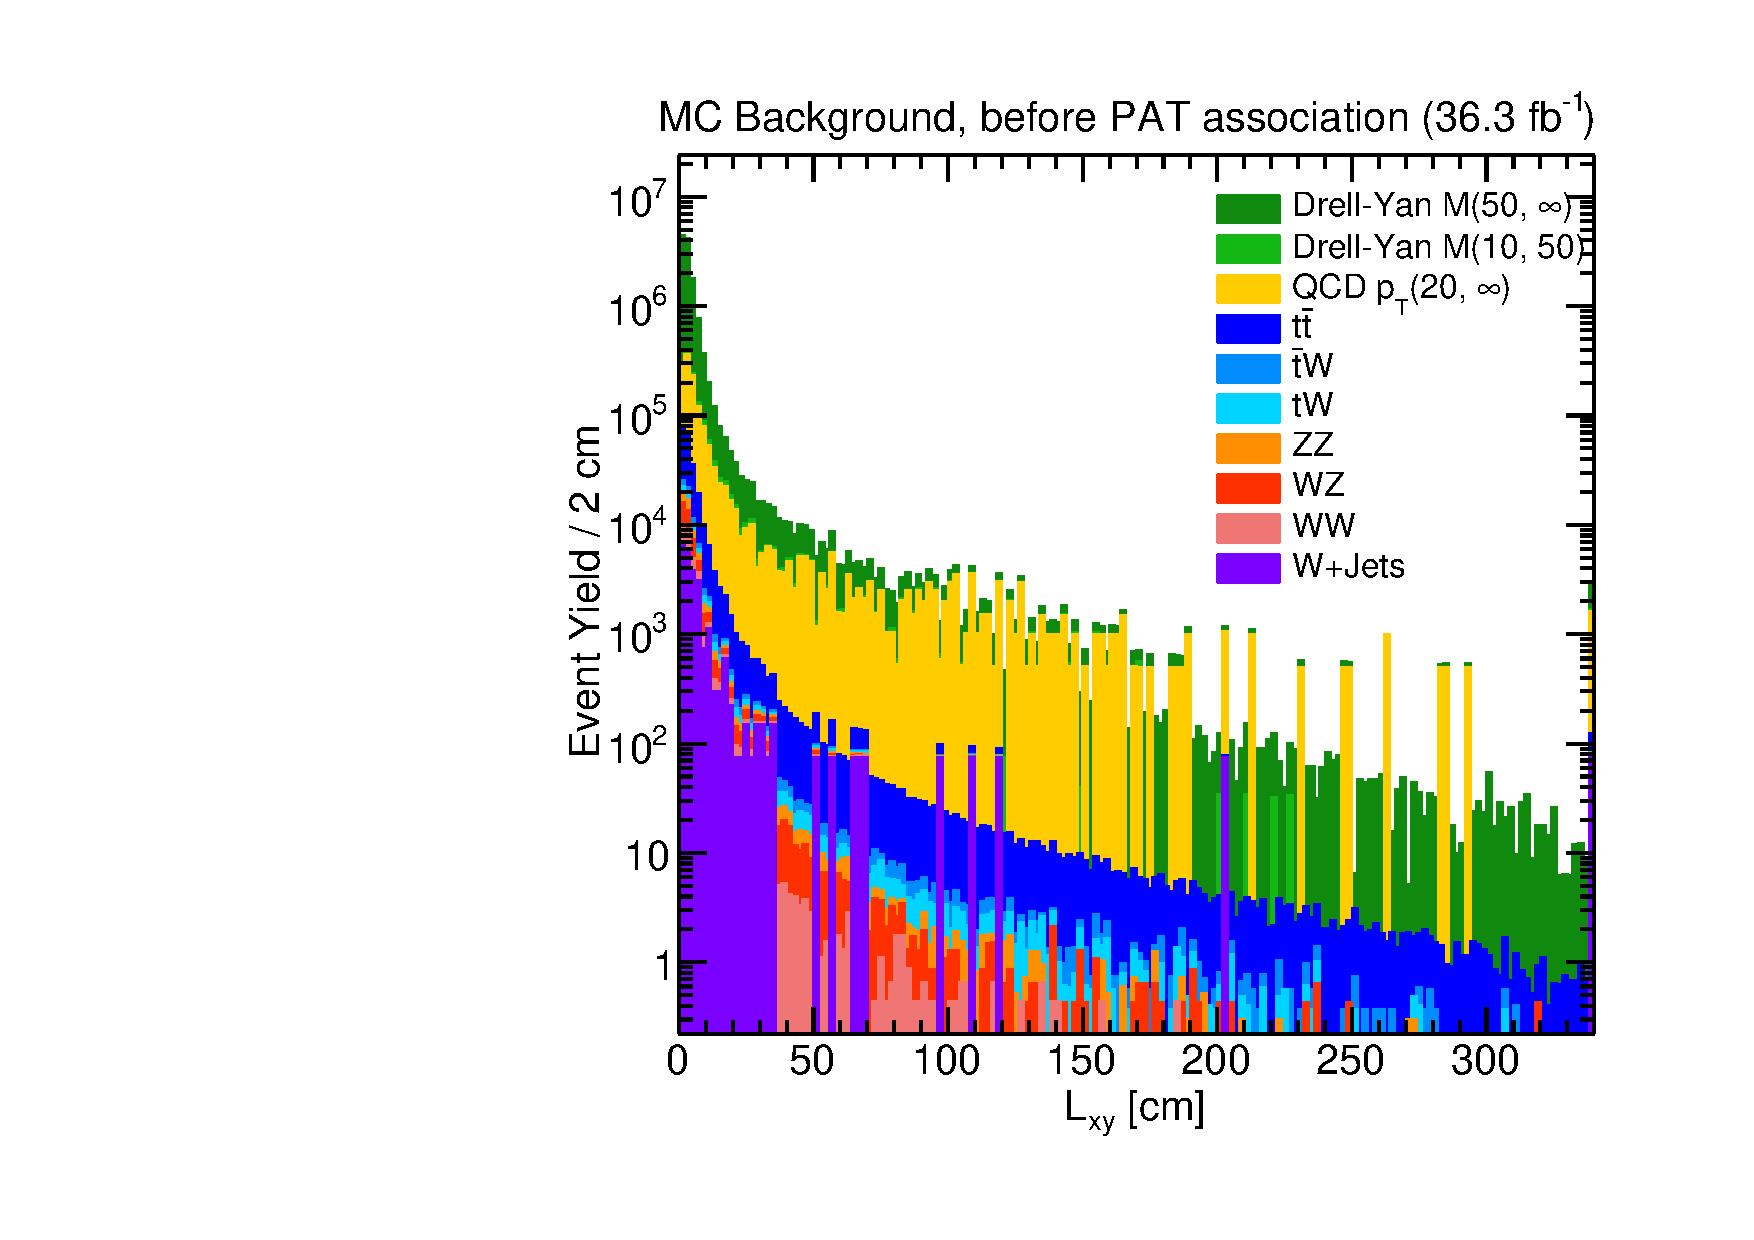
\includegraphics[width=\DSquareWidth]{figures/displaced/REPEFF_MC_Lxy-before.pdf}
  \hspace*{-2em}
  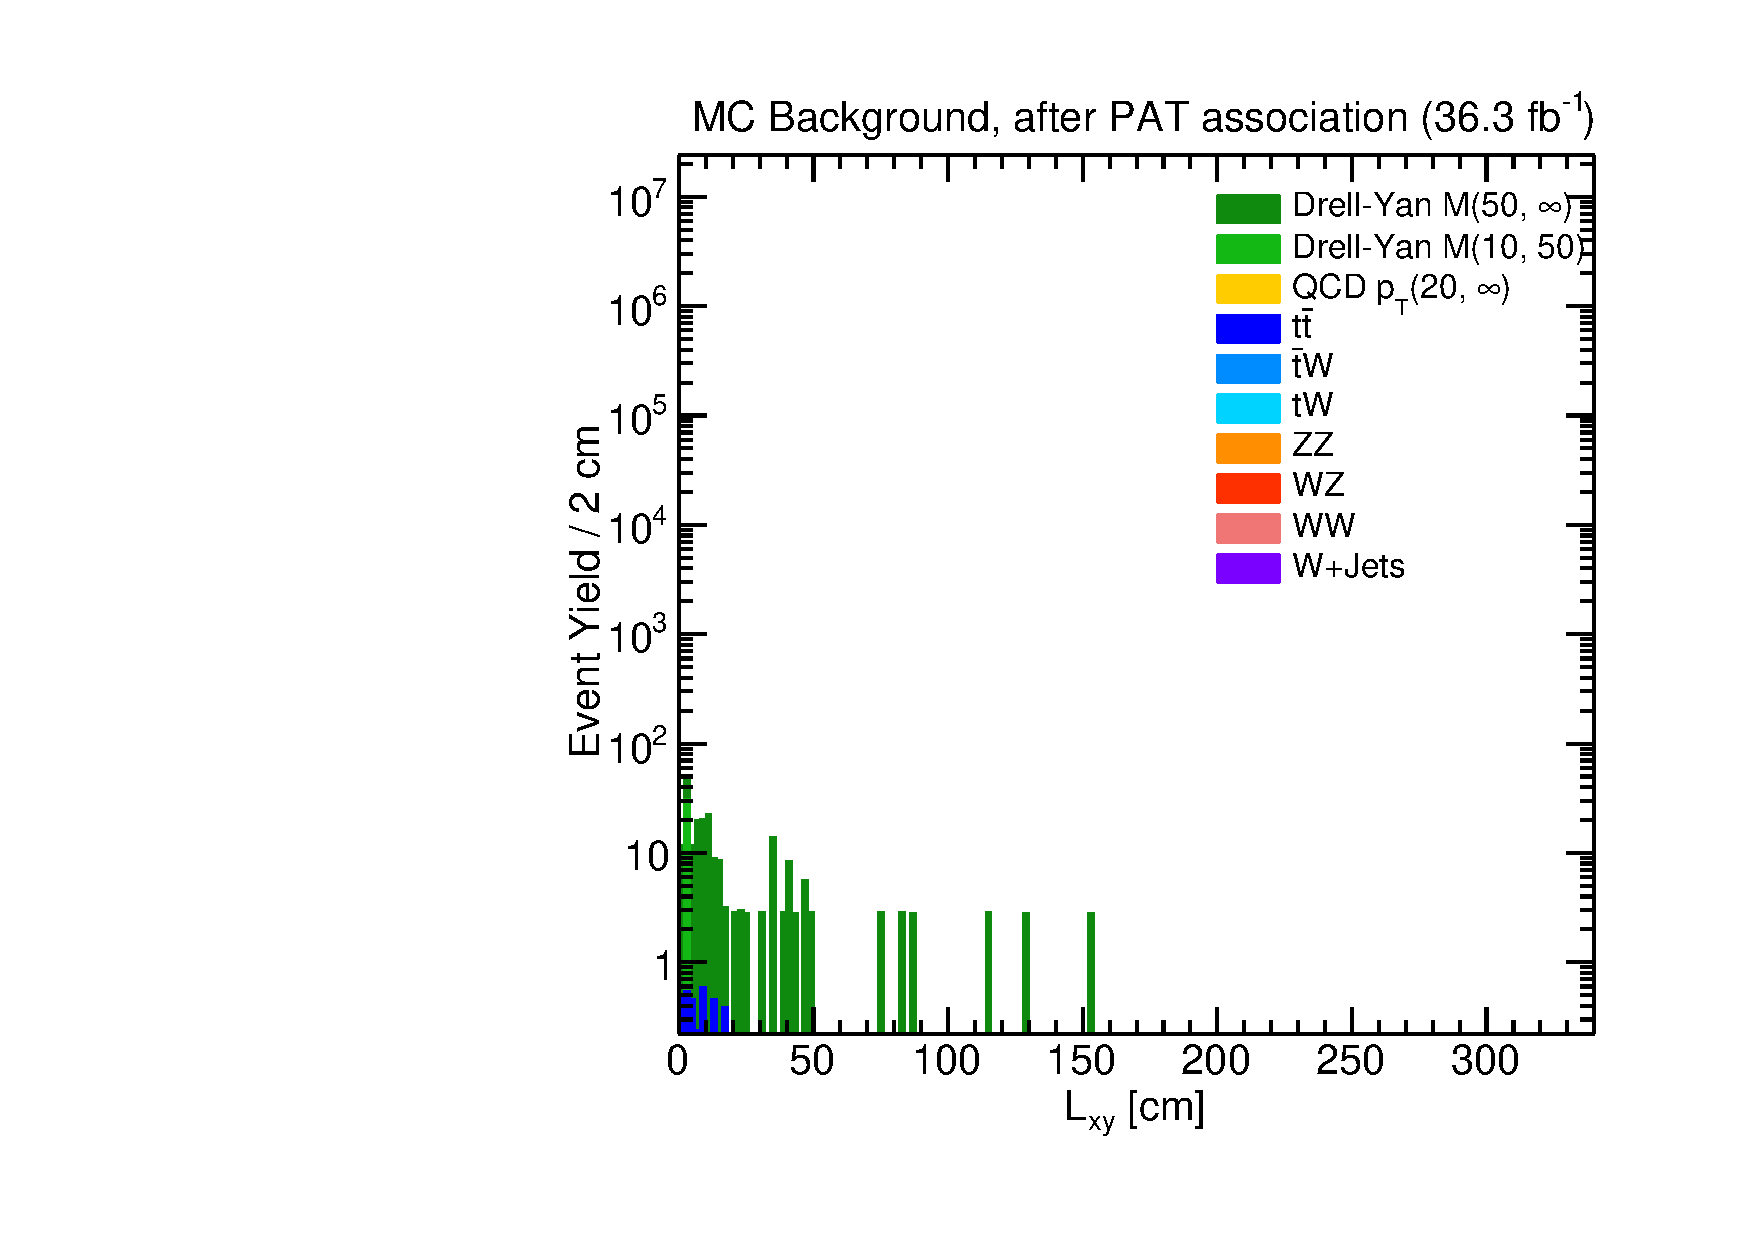
\includegraphics[width=\DSquareWidth]{figures/displaced/REPEFF_MC_Lxy-after.pdf}
  \caption[Histogram of dimuon \Lxy in simulated background samples before and after the PAT association procedure.]{Histogram of dimuon \Lxy in simulated background samples, scaled to 2016 integrated luminosity, \figpos{left} before and \figpos{right} after the PAT association procedure. The procedure suppresses the number of background events by a factor of $10^5$.}
  \label{fig:dd:REPEFF_MC_Lxy}
\end{figure}

In contrast, the association procedure essentially leaves true signal events with dimuon decays outside the tracker relatively untouched.
\Fig~\ref{fig:dd:REPEFF_Signal_Lxy} is a graph of the number of dimuons (matched to generated signal muons by choosing the closest DSA muons to each generated muon in a cone of $\deltaR < 0.2$ between their momentum directions) remaining after PAT association (\ie composed of DSA muons not associated with PAT muons), divided by the number of dimuons before PAT association, as a function of generated \Lxy.
In order to have a sufficient sample size, all 33 of the \twoMu signal samples are combined together for these graphs.
The association efficiently rejects signal events with decays inside the tracker volume, $\Lxy < 65\cm$, while rejecting no more than 10\% of signal events with decays outside the tracker volume, $\Lxy > 65\cm$.
\begin{figure}[htpb]
  \centering
  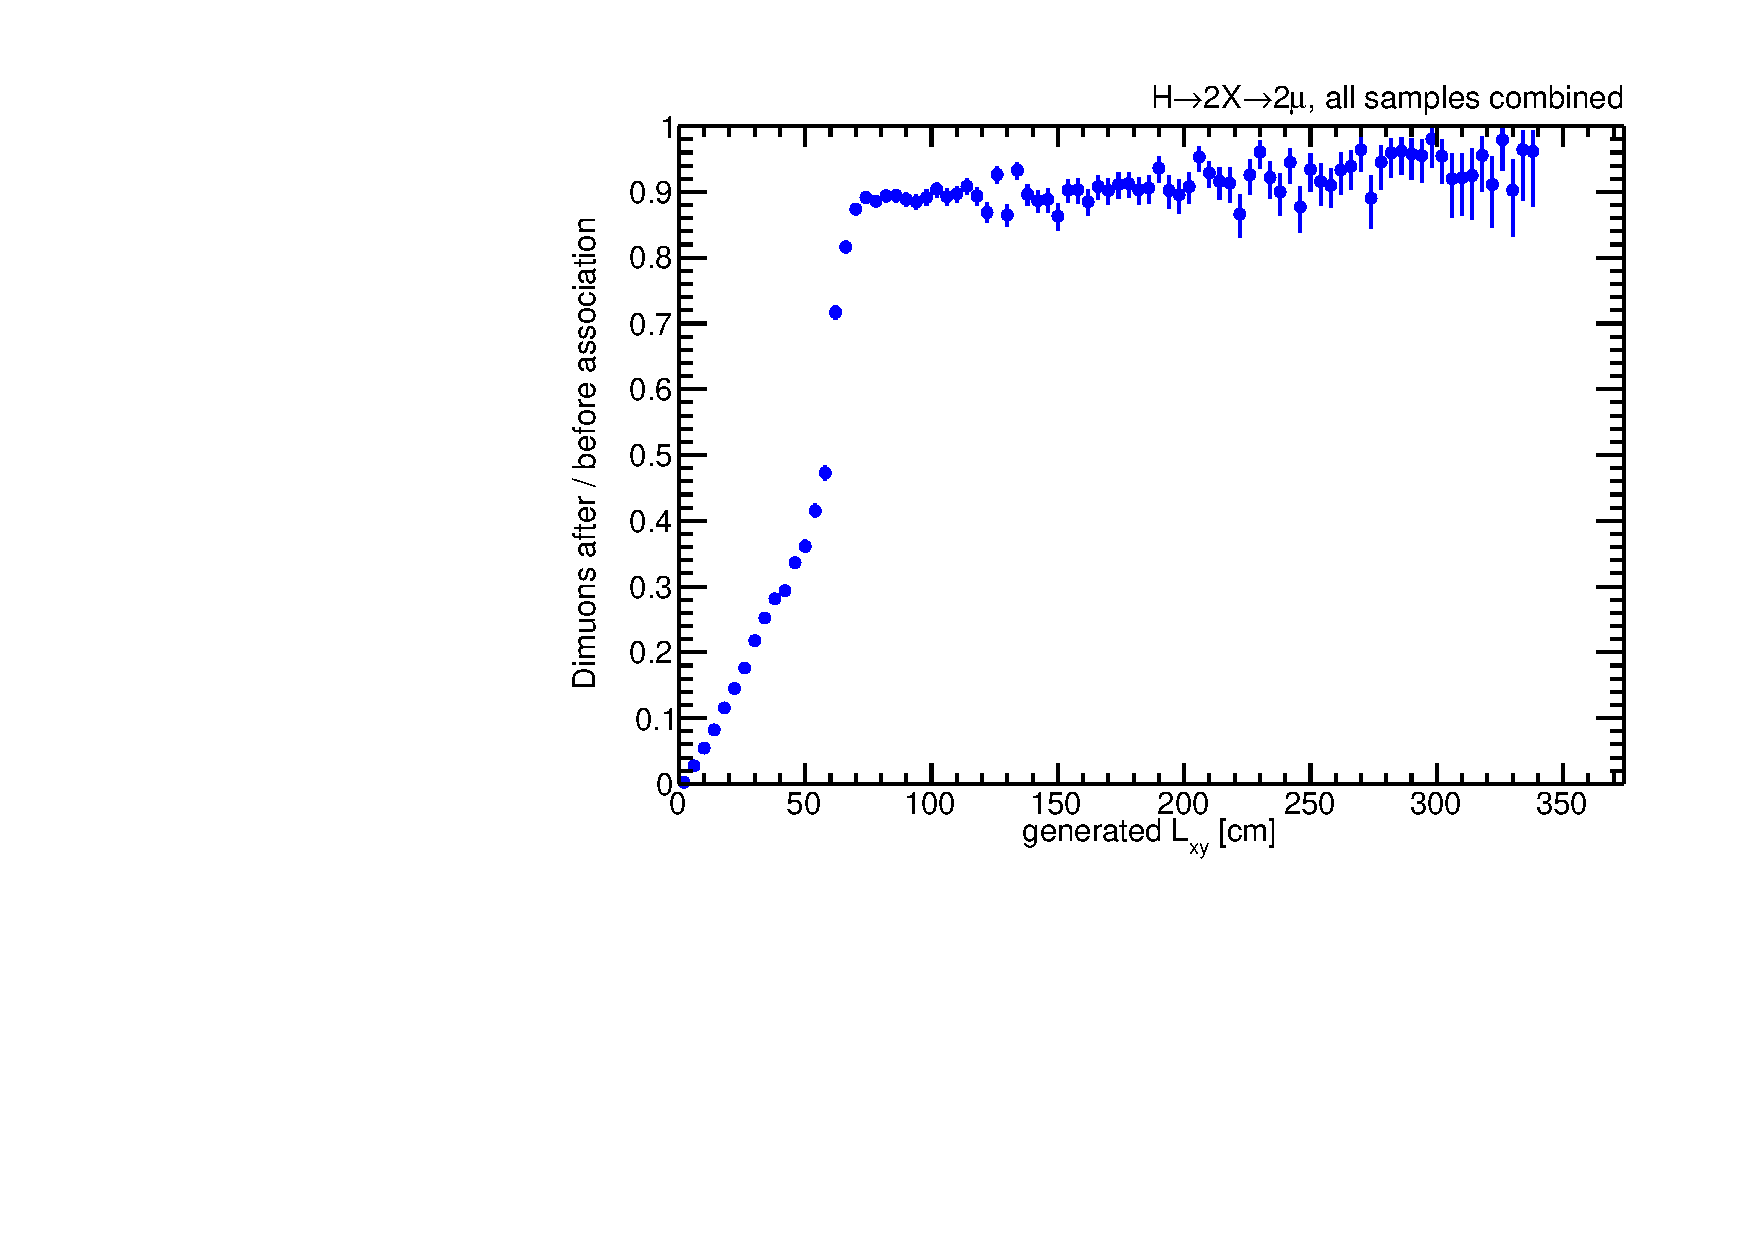
\includegraphics[width=\DFigWidth]{figures/displaced/REPEFF_Signal_Global.pdf}
  \caption[Graph of the number of dimuons after the PAT association divided by the number of dimuons before the PAT association, as a function of generated \Lxy, in all \twoMu signal samples combined.]{Graph of the number of dimuons after the PAT association divided by the number of dimuons before the PAT association, as a function of generated \Lxy, in all \twoMu signal samples combined. This graph shows that the association performs as expected, primarily rejecting signal events whose decays occurred within the tracker volume, while accidentally replacing no more than 10\% of events outside the tracker volume.}
  \label{fig:dd:REPEFF_Signal_Lxy}
\end{figure}


\subsection{DSA Muon Object Selection}
\label{sec:dd:DSAObject}
After the \DSAToPAT association step explained in the previous section, the analysis considers DSA muons not associated with any PAT muons.
As DSA muons are not used by many CMS analyses, a standard set of selections to identify DSA muons does not exist.
In order to further select high-quality DSA muons as well as to discriminate signal-like events from background-like events, the following requirements, along with the DSA muon preselection cuts explained in \Sec~\ref{sec:dd:DSAQuality}, serve as the DSA muon identification selection.
DSA muons are required to have
\begin{itemize}
  \item muon $\pT$ of at least 10\GeV, \ie $$\pT > 10\GeV$$
  \item \normchisq of the muon track fit of at most 2.5, \ie $$\chisq_\text{track}/\text{dof} < 2.5$$
  \item at least 19 hits in the DTs for muons reconstructed only in the barrel, \ie $$N(\text{CSC hits}) = 0 \implies N(\text{DT hits}) > 18$$
  \item time with respect to bunch crossing of at most 12\unit{ns}, \ie $$|t_\text{in-out}| < 12\unit{ns}$$
\end{itemize}

The \pT cut suppresses background events, which often have poor quality muons with low \pT, including background events arising from QCD processes.
The track \normchisq cut ensures that the muons are reasonably well reconstructed.
The $N(\text{DT hits})$ cut discriminates signal events from background events.
The timing cut is explained in \Sec~\ref{sec:dd:timing}.

\pagebreak
\subsubsection{In-Time with Triggering Bunch Crossing Requirement}
\label{sec:dd:timing}
A potentially pernicious class of events that can mimic displaced dimuon decays arises from a combination of technical features in the trigger and readout electronics of the muon chambers and the silicon tracker.
In a normal event with two muons, the timing of the trigger pulse from the two muons in the muon chambers is correctly aligned in time with the hit readout of the muon chambers and the tracker.
It can happen, however, that jitter in the muon trigger electronics creates a \Lone trigger signal that is 25\unit{ns} earlier than normal.
In the muon system readout, the muon hits are still recorded, but they have hit times that are 25\unit{ns} later than normal (since they are measured with respect to the \Lone trigger signal that is 25\unit{ns} too early).
When there is an early \Lone trigger signal, in contrast, the tracker hits associated with the triggering muons are \emph{not} recorded; tracker hits from unrelated \pp collisions 25\unit{ns} earlier are recorded instead.
The offline reconstruction code then finds the two triggering muons, but not the associated tracker tracks.
This mimics the main feature of displaced muons: tracks in the muon system with no associated tracker tracks.

Fortunately, the recorded times of the hits in the muon system provide a means to recognize such (very rare) events.
In practice, the time of the DSA muons is obtained from a precision timing algorithm that is implemented for standard standalone (SA) muons.
This algorithm provides a time that is centered on zero for normal muons, with jitter of a few nanoseconds, computed by extrapolating to the interaction point the times each constituent hit was formed with respect to the bunch crossing, under the hypothesis that the muon was produced in the detector and traveled outwards.
This time is referred to as $t_\text{in-out}$.

Matching DSA muons to SA muons is straightforward: DSA muons with an SA muon within a \deltaR cone of 0.2 are considered matched to the SA muon.
The time associated with the SA muon can be used to distinguish between normal muons and the pathological cases where the times are centered on non-zero multiples of 25\unit{ns} (the time between bunch crossings).
This requirement is implemented as the requirement $|t_\text{in-out}| < 12\unit{ns}$, and is more than 99\% efficient for simulated samples of the \twoMu signal.

\pagebreak
This class of background was understood only after unblinding the signal region, and so this selection criterion was added with the knowledge that it would eliminate some events.
However, we believe that this is a clear case that any bias due to adding this criterion is negligible, and that it would be foolish not to add this criterion, given our current understanding of this background.

\subsection{Dimuon Formation from Common Vertex Fit}
\label{sec:dd:DimVertex}
A decay of a long-lived particle to two muons is detected as a pair of muons originating from a common vertex, so at this stage, pairs of reconstructed muons are investigated together for consistency with originating from a common vertex and from the decay of a massive, long-lived particle.
A pair of DSA muon tracks fit to a common vertex, along with the four-momentum sum of the two muons, is referred to as a dimuon.
All $n(n-1)/2$ possible pairs of distinct DSA muons among $n$ selected DSA muons are initially considered when forming dimuons.
This set of pairs is immediately filtered by requiring that the distance of closest approach (DCA) of the two DSA tracks helically extrapolated in the magnetic field is less than 50\unit{cm}:
$$\text{DCA} < 50\unit{cm}$$
This is a loose requirement ensuring that the common vertex fit is not performed on a pair of tracks that never come close to approaching each other.

\subsubsection{Vertex Fitting}
\label{sec:dd:VertexFitting}
The common vertex fit is performed by an implementation of the Kalman filter algorithm in the CMS software, called the \Code{KalmanVertexFitter} \cite{Fruhwirth:1987fm,Speer:927395}.
The default implementation in the CMS software version used in this analysis restricts the range of the location of the fitted vertex to approximately within the boundary of the silicon tracker.
In this analysis, this restricted range is extended to the beginning of the muon system in order to efficiently reconstruct a common vertex for particles decaying outside the tracker.

The technical changes to the CMS software are documented here.
The following changes were made to \Code{RecoVertex/VertexTools/src/SequentialVertexFitter.cc}:
\begin{itemize}
  \item \Code{TrackerBoundsRadius} was changed from 112 to 500
  \item \Code{TrackerBoundsHalfLength} was changed from 273.5 to 1000
\end{itemize}

The results of the common vertex fit are used to define dimuon quantities such as transverse decay length.
As the existence of a common vertex fit is necessary to further study dimuon properties and consistency, the common vertex fit is required to converge.
The common vertex fit modifies the input tracks in order to be consistent with originating from a common vertex; these tracks are referred to as ``vertex-constrained'', and any of the muon properties (\pT, direction, \etc) may be different in the vertex-constrained version of the track than in the original version.
For many purposes, the vertex-constrained tracks are preferable because they represent a reconstruction performed with more information.
However, in a few situations, the vertex fitter fails or produces nonsensical results.
A few of the features of the fitter are documented here.

\begin{figure}[htpb]
  \centering
  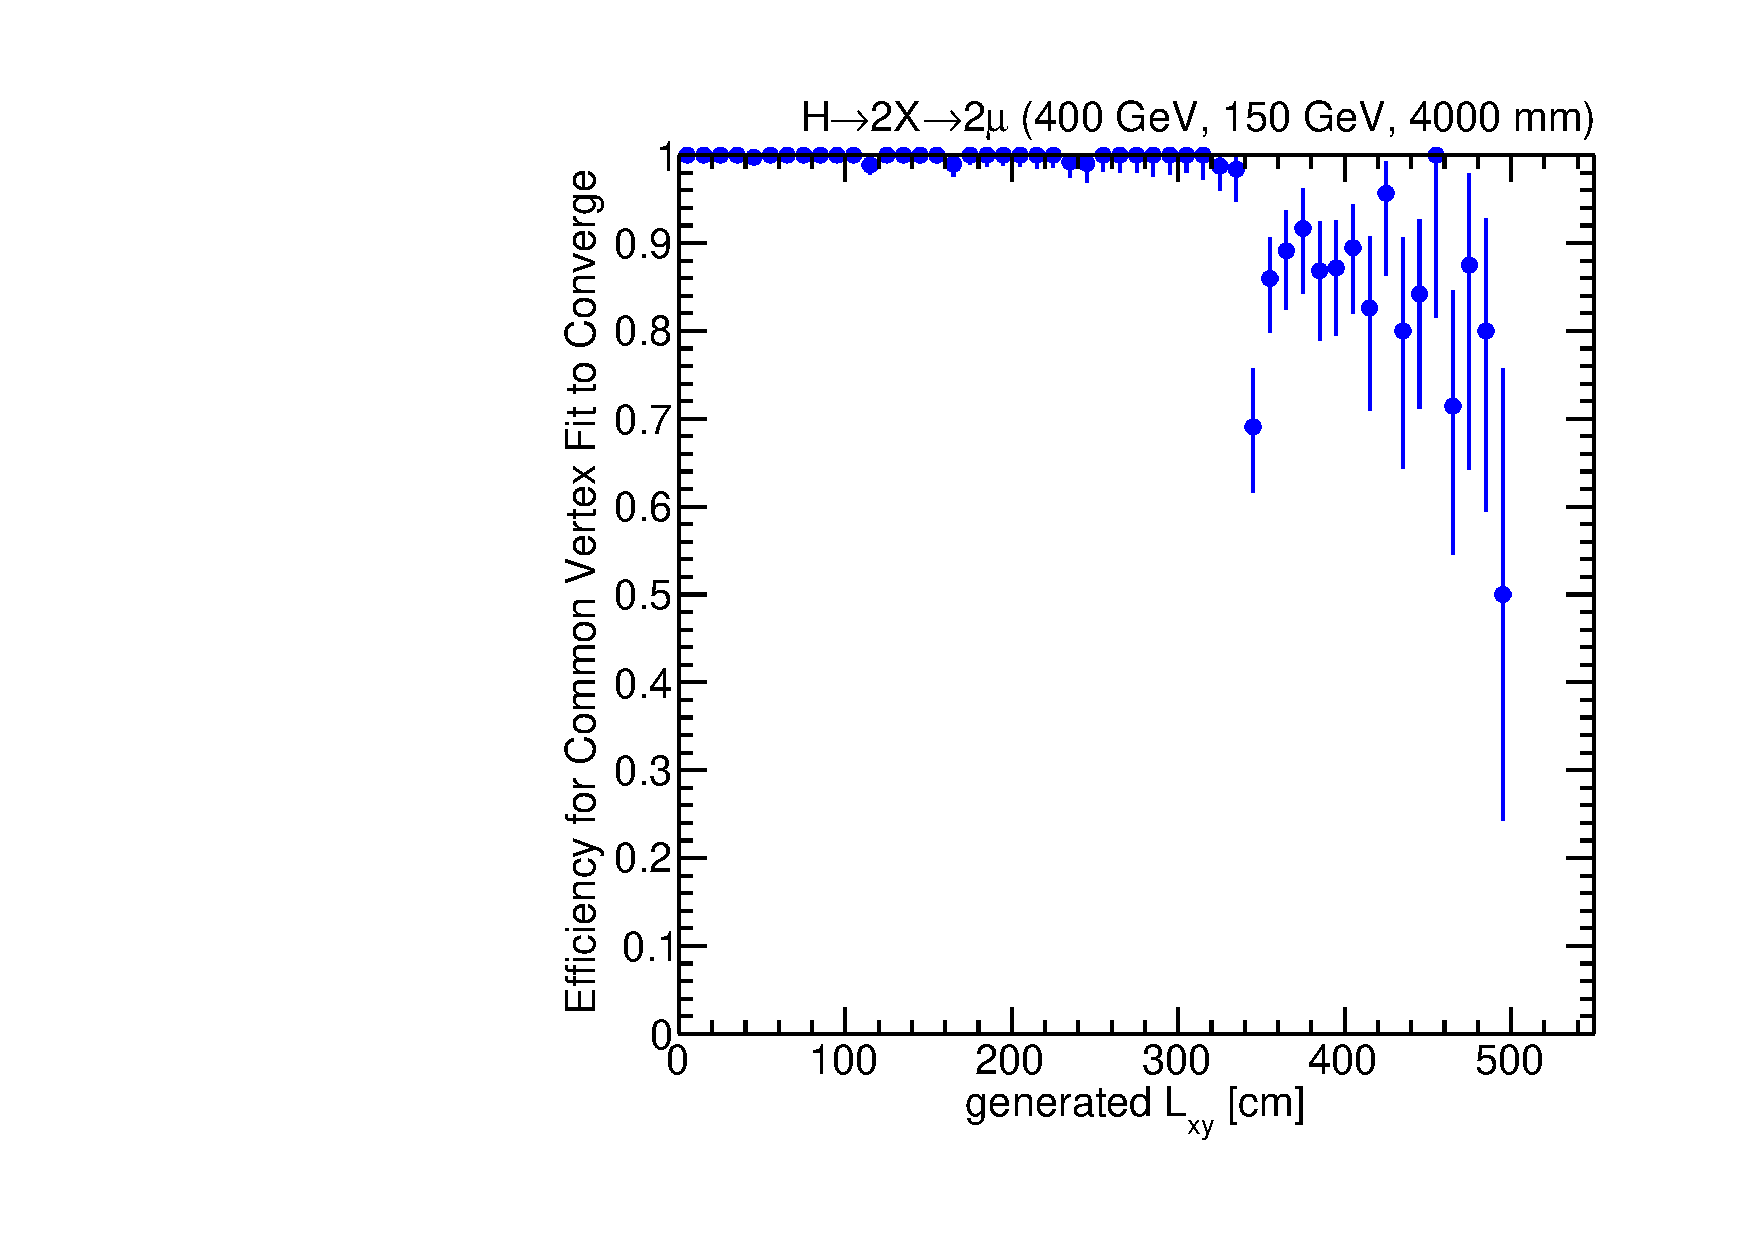
\includegraphics[width=\DSquareWidth]{figures/displaced/VFE_Lxy_2Mu2J_400_150_4000.pdf}
  \hspace*{-2em}
  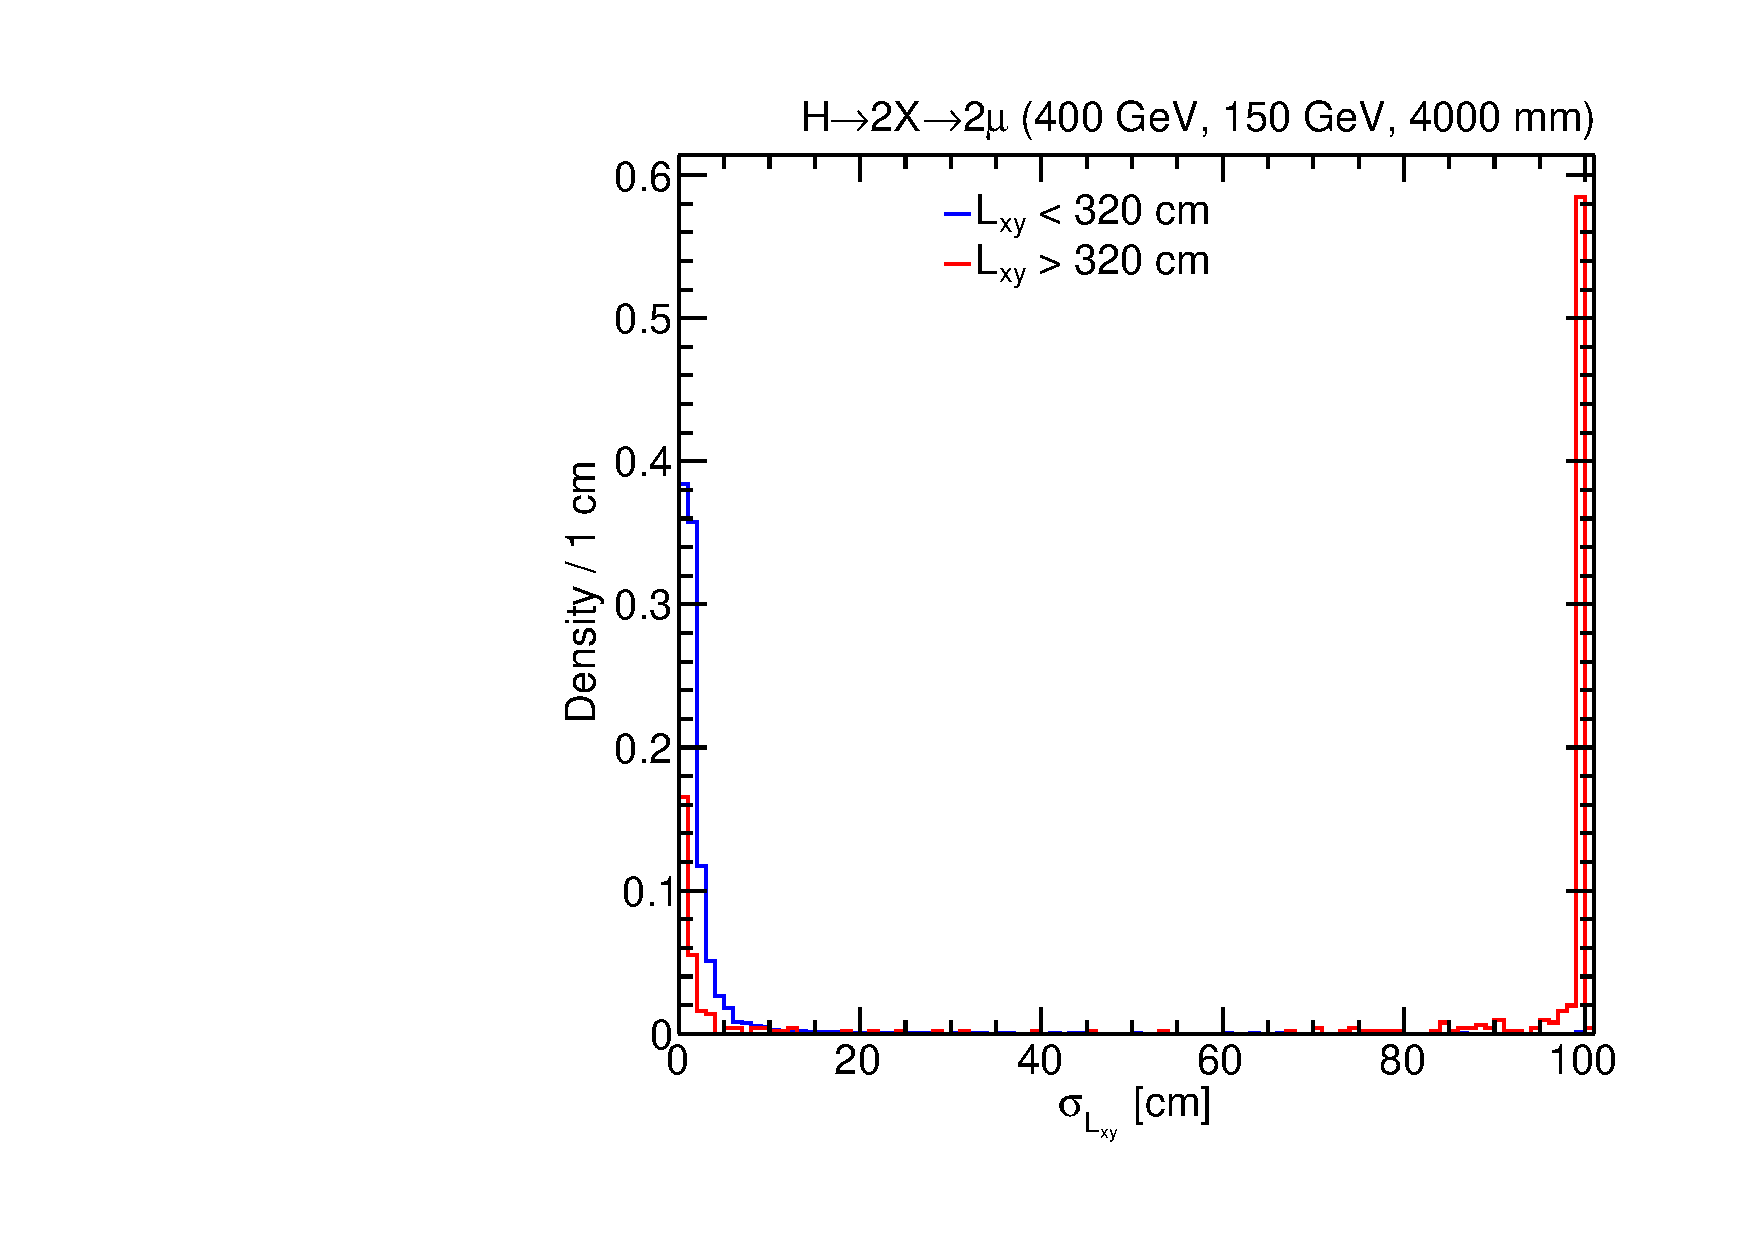
\includegraphics[width=\DSquareWidth]{figures/displaced/LESSMORE_LxyErr_2Mu2J_400_150_4000.pdf}
  \caption[Efficiency for the common vertex fit to converge as a function of generated \Lxy for generated events within acceptance and histograms of \LxyErr normalized to unit area for $\Lxy < 320\cm$ and $\Lxy > 320\cm$.]{\figpos{Left} Efficiency for the common vertex fit to converge for the \twoMu signal sample with \FullSP{400}{150}{4000} as a function of generated \Lxy, for generated events within acceptance. Both the preselection and object selection cuts are applied to DSA muons. In this graph, events are not required to pass the trigger, the HLT-RECO matching requirement was dropped, and the \DSAToPAT association procedure was not performed. Error bars are for the statistical uncertainty only. \figpos{Right} Histograms of \LxyErr normalized to unit area for the events in the numerator of the left plot, separately for $\Lxy < 320\cm$ and $\Lxy > 320\cm$, for the \twoMu signal sample with \FullSP{400}{150}{4000}, for generated events within acceptance. The distribution for $\Lxy > 320\cm$ has a large peak near 100\cm.}
  \label{fig:dd:VertexFitAnomalies}
\end{figure}

The vertex fit does not always converge for an arbitrary pair of tracks.
The left plot of \Fig~\ref{fig:dd:VertexFitAnomalies} is a graph of the efficiency for the common vertex fit to converge, with respect to signal events in which both generated muons are reconstructed as DSA muons, as a function of the generated \Lxy, for the \twoMu signal sample with \FullSP{400}{150}{4000}.

The denominator of this efficiency is the number of generated events within acceptance (both generated muon $\pT > 25\GeV$, both generated muon $|\eta| < 2$, and generated \mbox{$\Lxy < 500\cm$}) in which both generated muons had matching DSA muons.
That is, each generated muon has a DSA muon passing the muon preselection and the muon object selection within a cone of $\deltaR < 0.2$ between their momentum directions.
The numerator of this efficiency is the number of such events in which the dimuon common vertex fit converged for the two matched muons.
In order to observe the effect of the common vertex fit independently of the low trigger efficiency at large \Lxy, events are not required to pass the trigger and the HLT-RECO matching requirement was dropped.
In order to have a sufficient sample size, the \DSAToPAT association procedure was not performed.

Convergence of the vertex fit is highly efficient when fitting two DSA muon tracks that are matched to generated signal muons produced from long-lived particle decaying in the detector up to transverse displacements of 330\unit{cm}.
Beyond 330\unit{cm}, the efficiency for the common vertex fit to converge drops dramatically.

For those events beyond 330\unit{cm} that do converge, the fit quality is often quite poor, \eg the \pT resolutions of the vertex-constrained tracks are worse than before the fit.
Finally, many of these events retain an internal \Lxy uncertainty (\LxyErr) of a default value of 100\cm.
The right plot of \Fig~\ref{fig:dd:VertexFitAnomalies} shows distributions, normalized to unit area, of the events in the numerator of the left plot of \Fig~\ref{fig:dd:VertexFitAnomalies}, separately for $\Lxy < 320\cm$ and $\Lxy > 320\cm$.
A large fraction of the events with $\Lxy > 320\cm$ have \LxyErr near 100\cm.
Such events would have a small \Lxy significance (3 or less) and would not pass an analysis selection.
This type of common vertex fit failure would result in the loss of these events, even though the fit converged.

As in the Run~1 analyses, the trigger efficiency at such large \Lxy values is quite small, and the \LxySig selection discussed in \Sec~\ref{sec:dd:DimuonSignal} usually suppresses such events as well.
Therefore, further study of these events and attempts to rescue them from the behavior of the vertex fitter are of low priority for this analysis, and the underlying causes for this behavior remain a curiosity.

\subsection{Pairing Criteria}
\label{sec:dd:PC}
Considering all possible pairs of DSA muons results in many dimuons formed from DSA muons that are not related in any way.
It is therefore important to develop criteria that choose the correct reconstructed dimuons with high efficiency, consistent with signal.
Selections on individual dimuons (such as requiring the \vchisq to be small) impose some quality constraints that are useful for selecting such dimuons, but any set of criteria that determines which pairs of muons form the correct dimuons must consider the event as a whole.
Choosing such a set of pairing criteria is particularly subtle in, for example, decays of two long-lived particles into a final state with 4 muons.
The 4 muons can be nominally paired into 6 overlapping dimuons, which can be partitioned into three distinct sets of 2 dimuons with no shared muons; the criteria must choose between them.
This situation is made more complex when, among other things,
\begin{itemize}
  \setlength\itemsep{.2\baselineskip}
  \item one or more muons are not reconstructed
  \item duplicate muons are reconstructed from partial sets of hits
  \item muons are not all reconstructed with the correct charge
  \item pairs of muons are highly collimated and distinguishing them is difficult
  \item vertex fits of muons from different long-lived particle decays yield a good \vchisq
\end{itemize}
In developing this set of pairing criteria, several combinations of metrics were considered.
\begin{itemize}
  \setlength\itemsep{.2\baselineskip}
  \item Dimuon(s) formed from the highest \pT muons in the event
  \item Dimuon(s) with the least \vchisq in the event
  \item Dimuon(s) formed from muons with charges of opposite sign
  \item Pairs of dimuons with the least sum of \vchisq
  \item Pairs of dimuons with the least difference in reconstructed dimuon mass
\end{itemize}
\Fig~\ref{fig:dd:pc} is a diagram illustrating the application of the pairing criteria to the set of all possible dimuons in the case of four selected muons.
\begin{figure}[htpb]
  \centering
  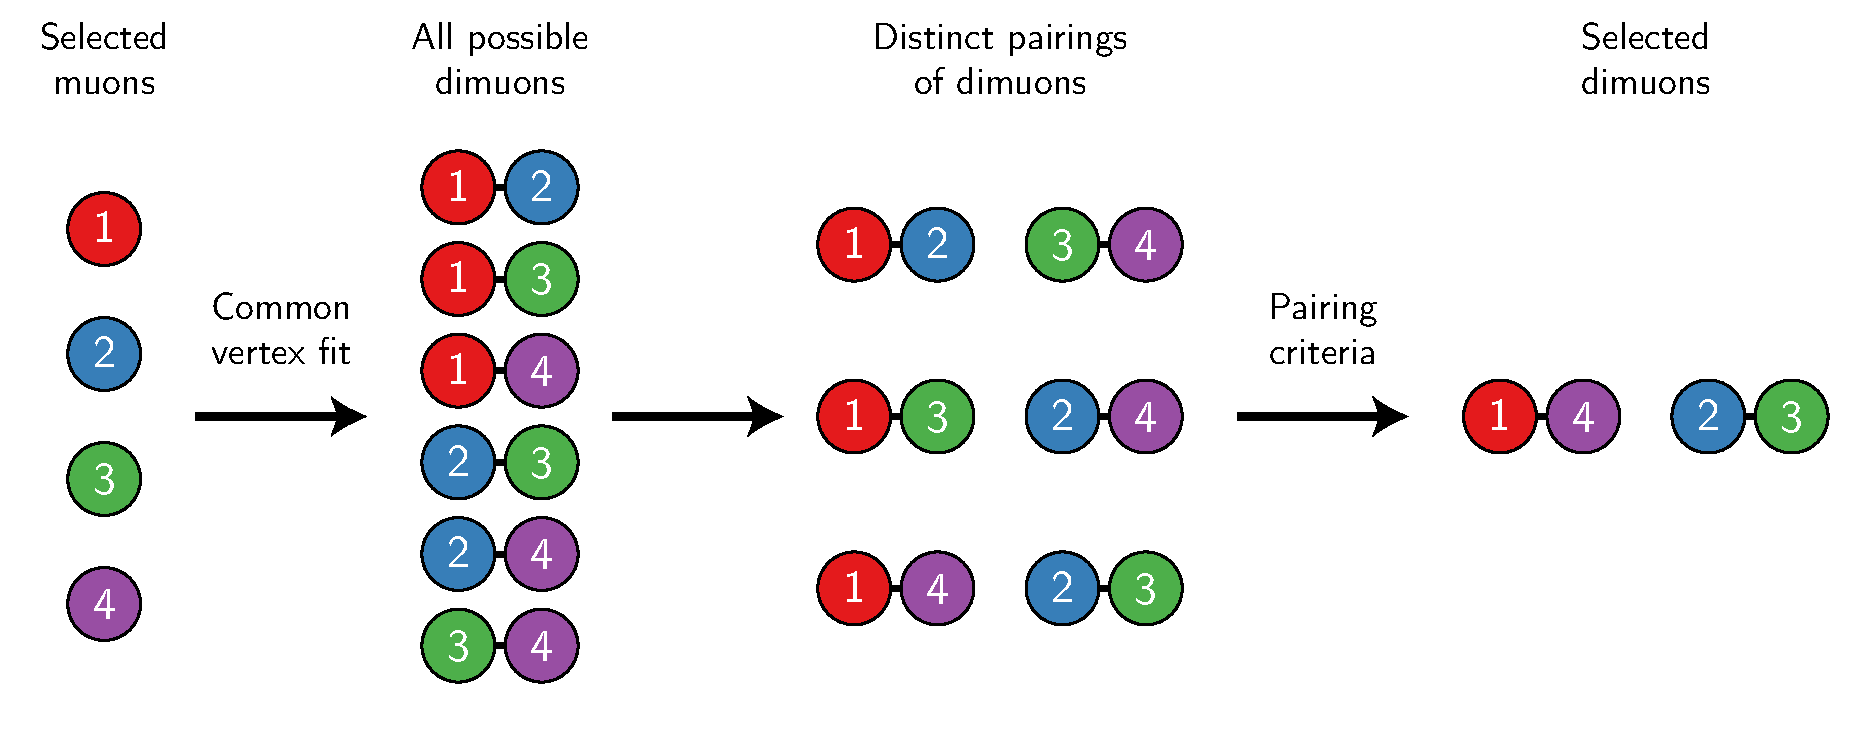
\includegraphics[width=\textwidth]{figures/displaced/PairingCriteriaDiagram.pdf}
  \caption[Diagram illustrating the application of pairing criteria to dimuons in the case of four selected muons.]{Diagram illustrating the application of pairing criteria to dimuons in the case of four selected muons. Four muons may be paired into six dimuons whose constituent muons overlap. These six dimuons may be partitioned into three distinct pairings of dimuons, in which no muons are shared between dimuons. Pairing criteria select the correct pair of dimuons consistent with a four muon signal event.}
  \label{fig:dd:pc}
\end{figure}

Potential pairing criteria were studied and optimized on both the \twoMu and \fourMu simulated signal samples.
Choosing the highest \pT muons in the event is highly correlated with choosing the signal muons, a fact that is robust across all signal sample parameters covering a wide range of long-lived particle lifetimes and muon \pT spectra.
Requiring that dimuons be formed from muons of opposite charge provides only modest efficiency gains with respect to choosing the signal dimuons, and is undesirable at this stage as it introduces dependence on a specific type of signal model.
In events with fewer than four muons, a simple ranking of all possible dimuons by \vchisq yielded the highest efficiency.

The combinatorial space is far richer in events with four or more muons.
For long-lived particles decaying outside the tracker leading to events with at least 4 muons, the criterion yielding the highest efficiency to select signal dimuons is to choose the pair of dimuons whose \vchisq sum is the smallest, among all distinct pairs of dimuons that can be formed from the 4 highest \pT muons in the event. 
An alternative criterion to the least sum of \vchisq is the least difference in reconstructed dimuon mass.
Due to the limited mass resolution of DSA muons, this criterion was found to be less efficient overall than the least sum of \vchisq, except in events with a generated transverse decay length of less than 30\unit{cm}, a region where this DSA muon-based analysis has low sensitivity.
Applying the pairing criteria to an event with any number of dimuons formed from any number of muons results in 2 or fewer selected dimuons for the event.
The full technical details of this procedure are depicted in \Fig~\ref{fig:dd:pca}.

\begin{figure}[htpb]
  \centering
  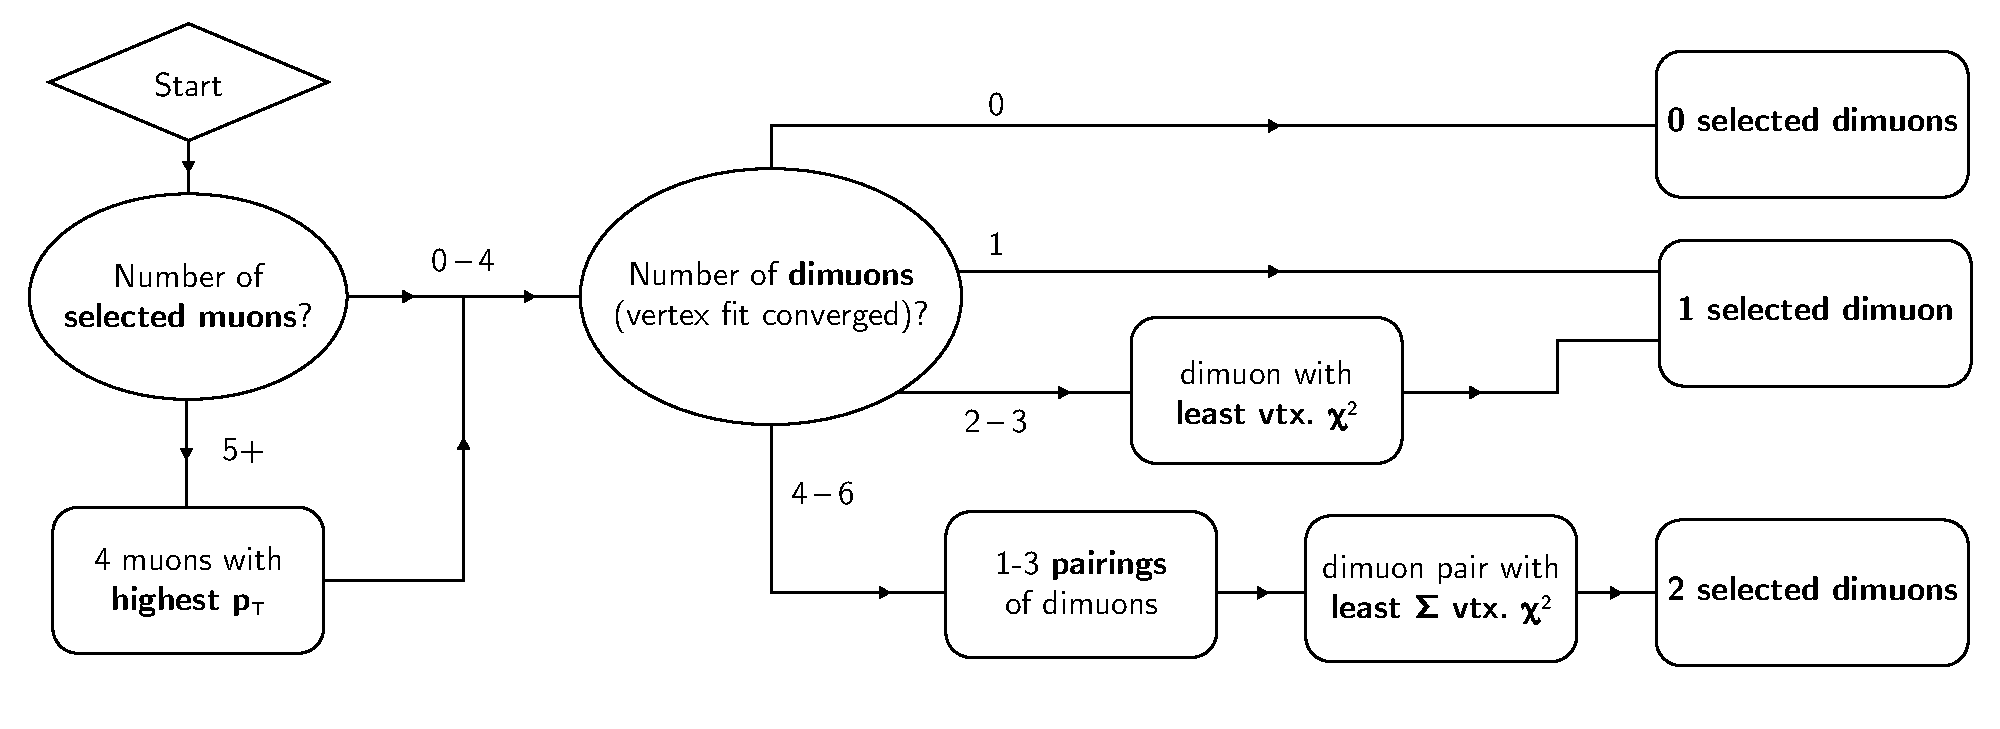
\includegraphics[width=\textwidth]{figures/displaced/PairingCriteriaAlgorithm.pdf}
  \caption[Flowchart depicting the technical details of the pairing criteria procedure.]{Flowchart depicting the technical details of the pairing criteria procedure. Up to 4 DSA muons are selected, ranked by \pT. With the DCA and vertex fit convergence requirements, these muons can be formed into up to 6 dimuons (0 for 0 or 1 muon, up to 1 for 2 muons, up to 3 for 3 muons, and up to 6 for 4 muons). The pairing criteria choose up to 2 dimuons among the possible dimuons.}
  \label{fig:dd:pca}
\end{figure}

\Fig~\ref{fig:dd:PC_Eff} shows graphs of the efficiency for the pairing criteria to correctly select reconstructed dimuons as a function of generated \Lxy, for a selection of \twoMu and \fourMu signal samples.
\Fig~\ref{fig:dd:PC_Eff_Global} shows the same graphs, but for all 33 signal samples combined together.
The denominator of this efficiency is the number of generated signal dimuons matching a reconstructed dimuon (using the closest DSA muons to each generated muon in a cone of $\deltaR < 0.2$ between their momentum directions).
The numerator of this efficiency is the number of reconstructed dimuons chosen by the pairing criteria that are the same as the reconstructed dimuon matched to generated signal.
This efficiency is 97--100\% for \twoMu and 80--98\% for \fourMu signal samples with medium and long lifetimes, for generated transverse decay lengths of $\Lxy > 100 \cm$.
The pairing criteria are less efficient for \fourMu samples with larger values of \mH and smaller values of \mX, because events in such samples consist of two pairs of highly collimated muons, which yield a greater uncertainty in the fitted vertex position in the dimuon momentum direction, and therefore less discriminating vertex \chisq values.

\begin{figure}[p]
  \centering
  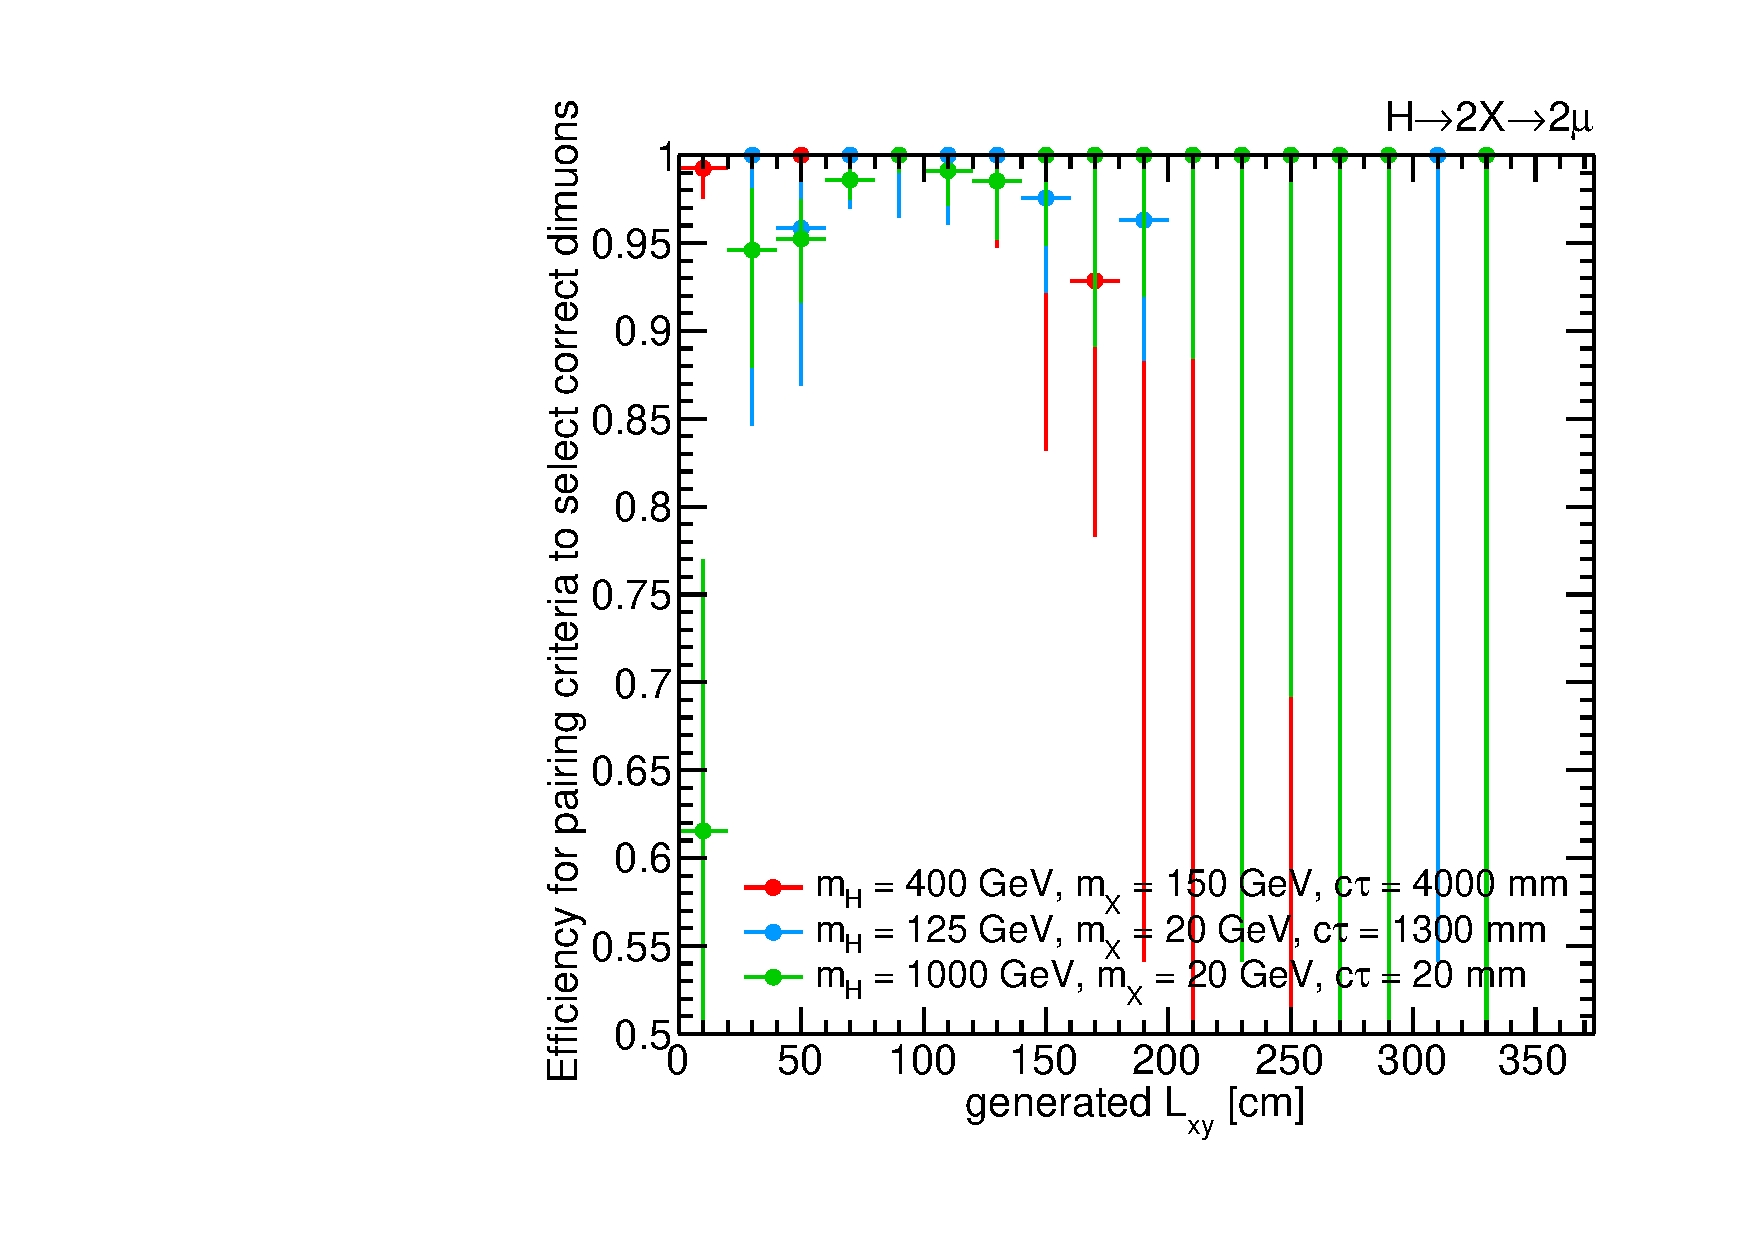
\includegraphics[width=\DSquareWidth]{figures/displaced/PC_Lxy_2Mu2J_Mul.pdf}
  \hspace*{-2em}
  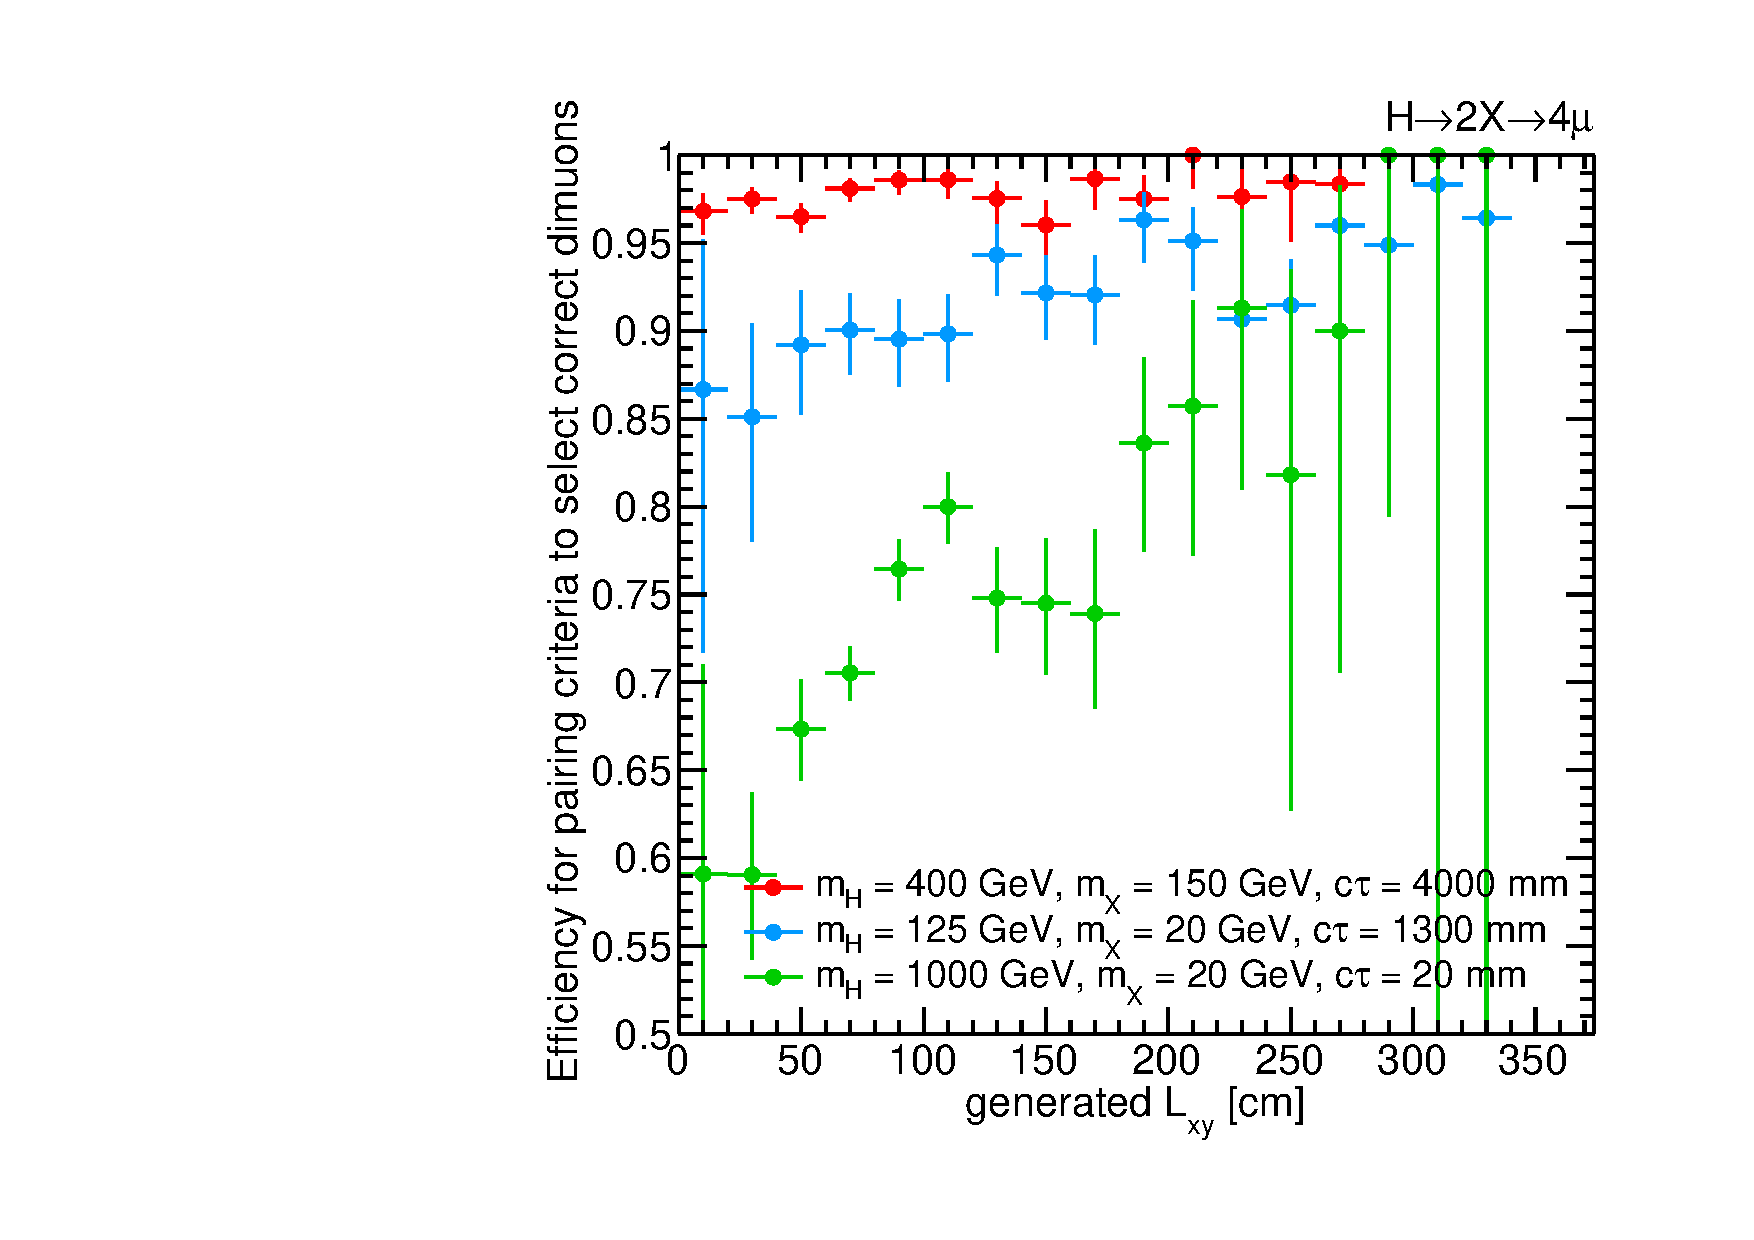
\includegraphics[width=\DSquareWidth]{figures/displaced/PC_Lxy_4Mu_Mul.pdf}
  \caption[Efficiency for the pairing criteria to correctly choose reconstructed dimuons as a function of generated \Lxy for \twoMu and \fourMu signal samples.]{Efficiency for the pairing criteria to correctly choose reconstructed dimuons as a function of generated \Lxy for \figpos{left} \twoMu signal samples and \figpos{right} \fourMu signal samples, for selected signal parameters. The behavior varies with signal parameters, and is lower for \fourMu signal samples, but overall the efficiency is high outside the tracker volume ($\Lxy > 100\cm$).}
  \label{fig:dd:PC_Eff}
\end{figure}
\begin{figure}[p]
  \centering
  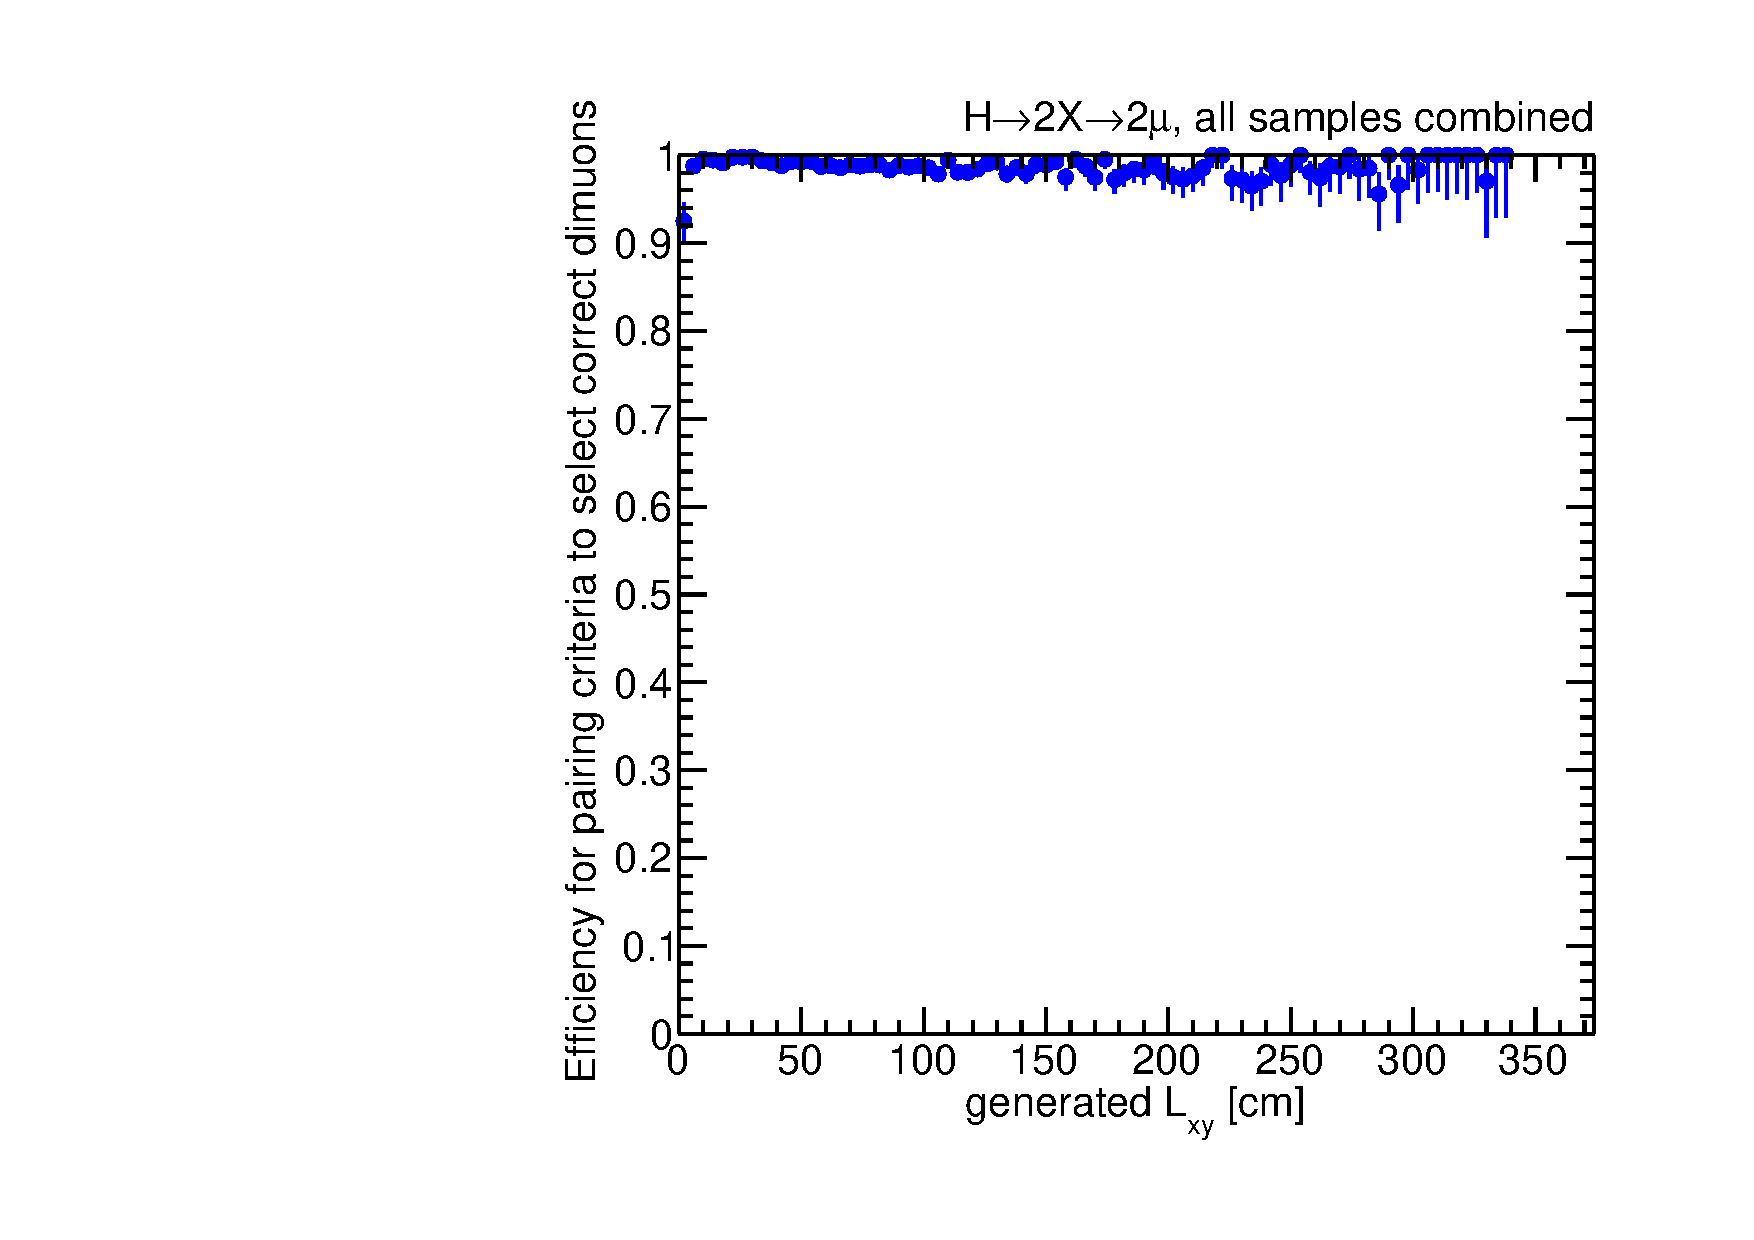
\includegraphics[width=\DSquareWidth]{figures/displaced/PC_Lxy_2Mu2J_Global.pdf}
  \hspace*{-2em}
  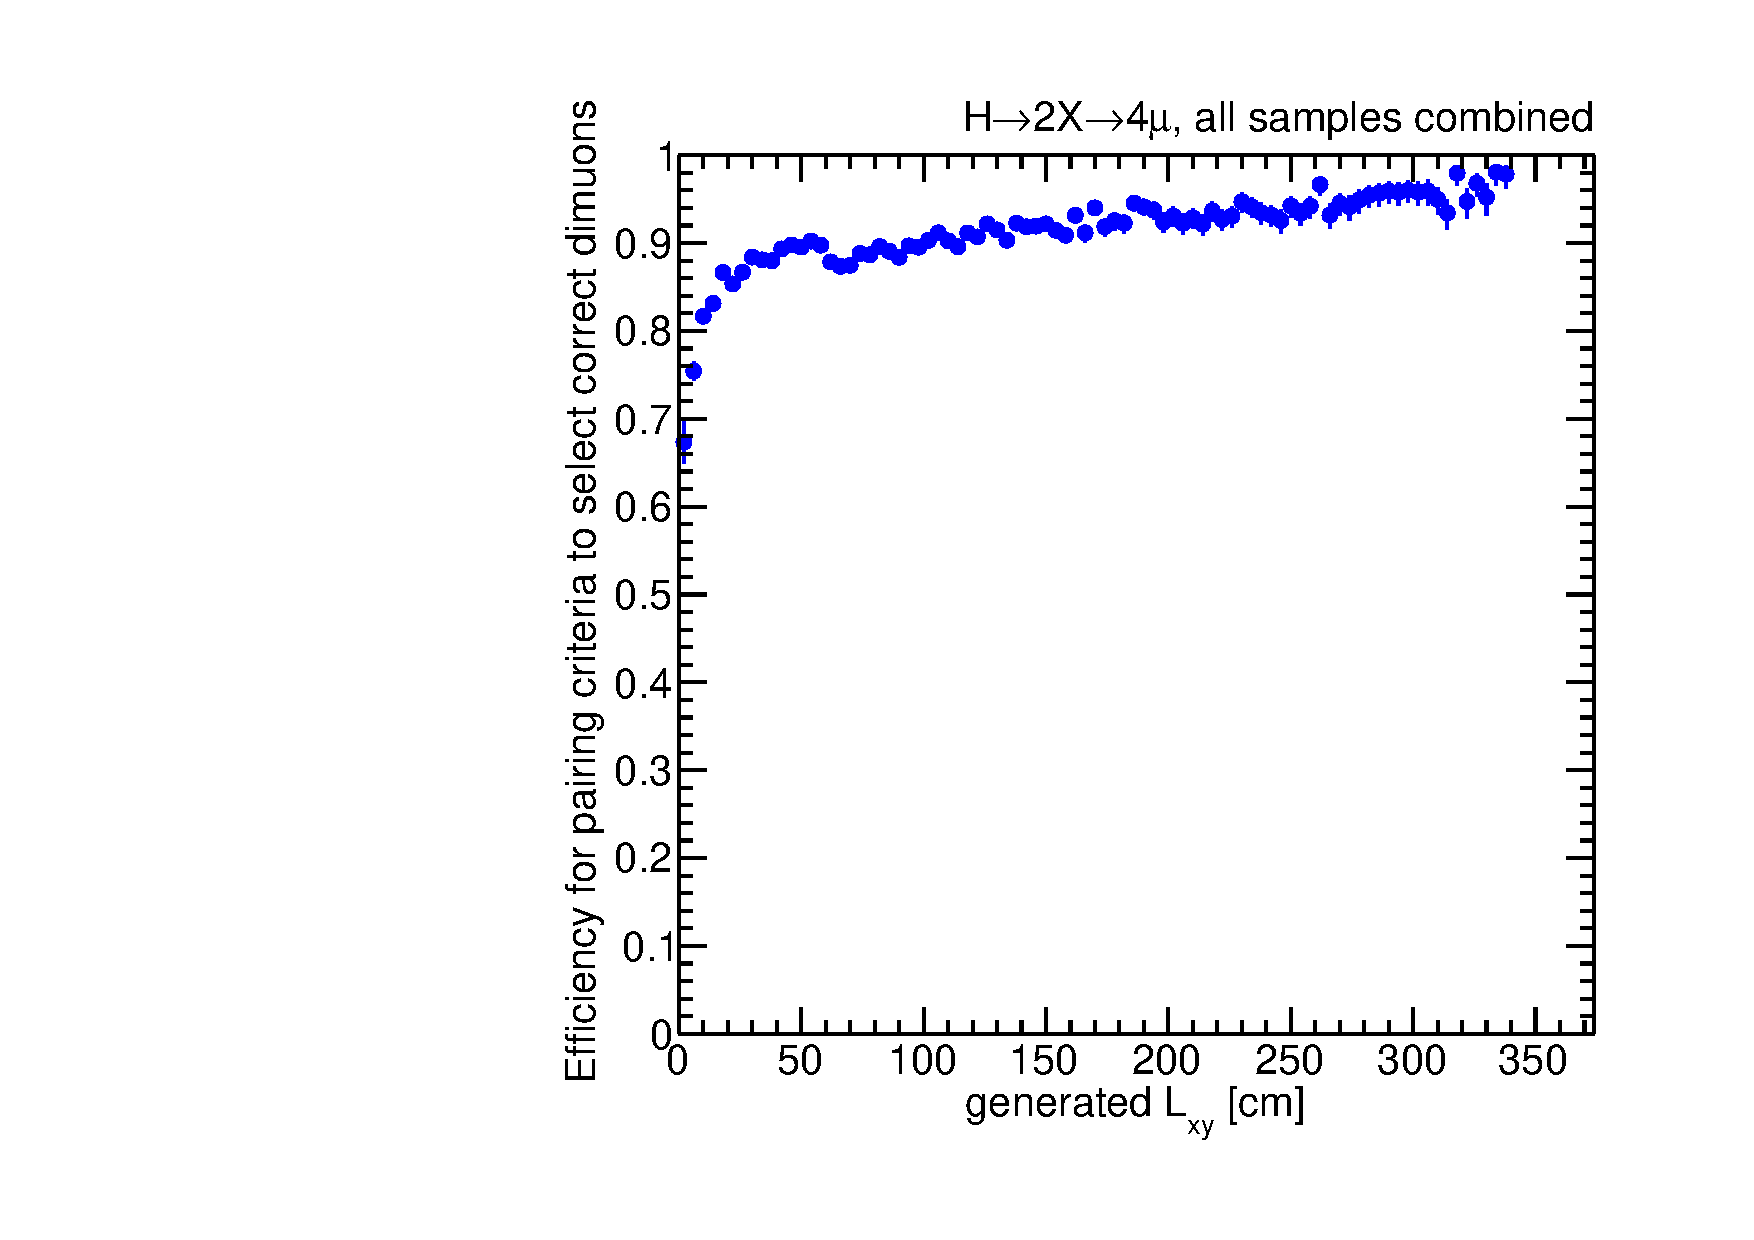
\includegraphics[width=\DSquareWidth]{figures/displaced/PC_Lxy_4Mu_Global.pdf}
  \caption[Efficiency for the pairing criteria to correctly choose reconstructed dimuons.]{Efficiency for the pairing criteria to correctly choose reconstructed dimuons, as in \Fig~\ref{fig:dd:PC_Eff}, for all samples combined.}
  \label{fig:dd:PC_Eff_Global}
\end{figure}

\subsection{Dimuon Object Selection}
\label{sec:dd:DimuonObject}
Along with the DCA requirement, the requirement of convergence of the common vertex fit, and the application of the pairing criteria explained in \Sec~\ref{sec:dd:PC}, the following requirements serve as a dimuon identification selection.
These requirements further select high-quality dimuons as well as suppress background events.
Dimuons are required:
\begin{itemize}
  \item to have a reconstructed dimuon mass of at least 10\GeV, \ie $\mMuMu > 10\GeV$
  \item to have a $\chi^2$ of the common vertex fit of at most 20, \ie $\chi^2_\text{vertex} < 20$
\end{itemize}

The \vchisq cut ensures that the dimuon is formed from tracks that can be reasonably well associated with a common vertex.
The mass cut suppresses complex backgrounds arising from QCD processes and events with low \pT and collimated muons.

\subsection{Dimuon Signal Selection}
\label{sec:dd:DimuonSignal}
The following criteria select displaced dimuons consistent with the signal hypothesis, \ie that the dimuon was constructed from two muons with opposite-sign charge originating from the decay of a long-lived particle produced promptly, resulting in a dimuon vertex displaced from the beam spot.
The relevant quantities were defined in \Sec~\ref{sec:dd:keyvars}.
Dimuons are required:
\begin{itemize}
  \item to have an \Lxy significance of at least 6, \ie $\LxySig > 6$
  \item to have a transverse collinearity angle of less than $\pi/4$, \ie $\DeltaPhi < \pi/4$
  \item to be formed from two DSA muons with electric charges of opposite sign
\end{itemize}

\subsection{Cosmic Muon Suppression}
\label{sec:dd:CosmicCuts}
As mentioned in \Sec~\ref{sec:dd:VertexFitting}, one result of the common vertex fit of two muons is a pair of vertex-constrained tracks.
After the common vertex fit, a population of selected dimuons with relatively small \vchisq values was observed in data, and not in simulation, with the following unusual properties, compared to before the common vertex fit:
\begin{itemize}
  \item Muon vertex-constrained momentum $\phi$ directions change by approximately $\pi$
  \item Muon vertex-constrained \pT uncertainties are unusually small, \ie $\pTErr/\pT \approx 10^{-7}\text{--}10^{-5}$
\end{itemize}
The presence of these dimuons are found to correlate with
\begin{itemize}
  \item Muons with relatively large transverse impact parameters, \ie $d_0 \approx 200\text{--}1000\cm$, and
  \item Events with no \pp collision vertices, and/or
  \item Events with large numbers of DSA muons, \ie $N(\text{DSA}) \approx 15\text{--}20$
    \begin{itemize}
      \item And these large numbers of DSA muons are largely parallel, \ie $|\cos{\alpha}| \approx 1$
    \end{itemize}
\end{itemize}
Further investigation suggested that these events are consistent with multiple cosmic muons arriving simultaneously from a single atmospheric shower.
\Fig~\ref{fig:dd:shower} is an example display of an event in data consistent with multiple cosmic muons from a single shower in a \pp collision event, containing a large number of approximately parallel pairs of DSA muons in addition to two global muons (not selected) originating from the \pp collision.

\begin{figure}[htpb]
  \centering
  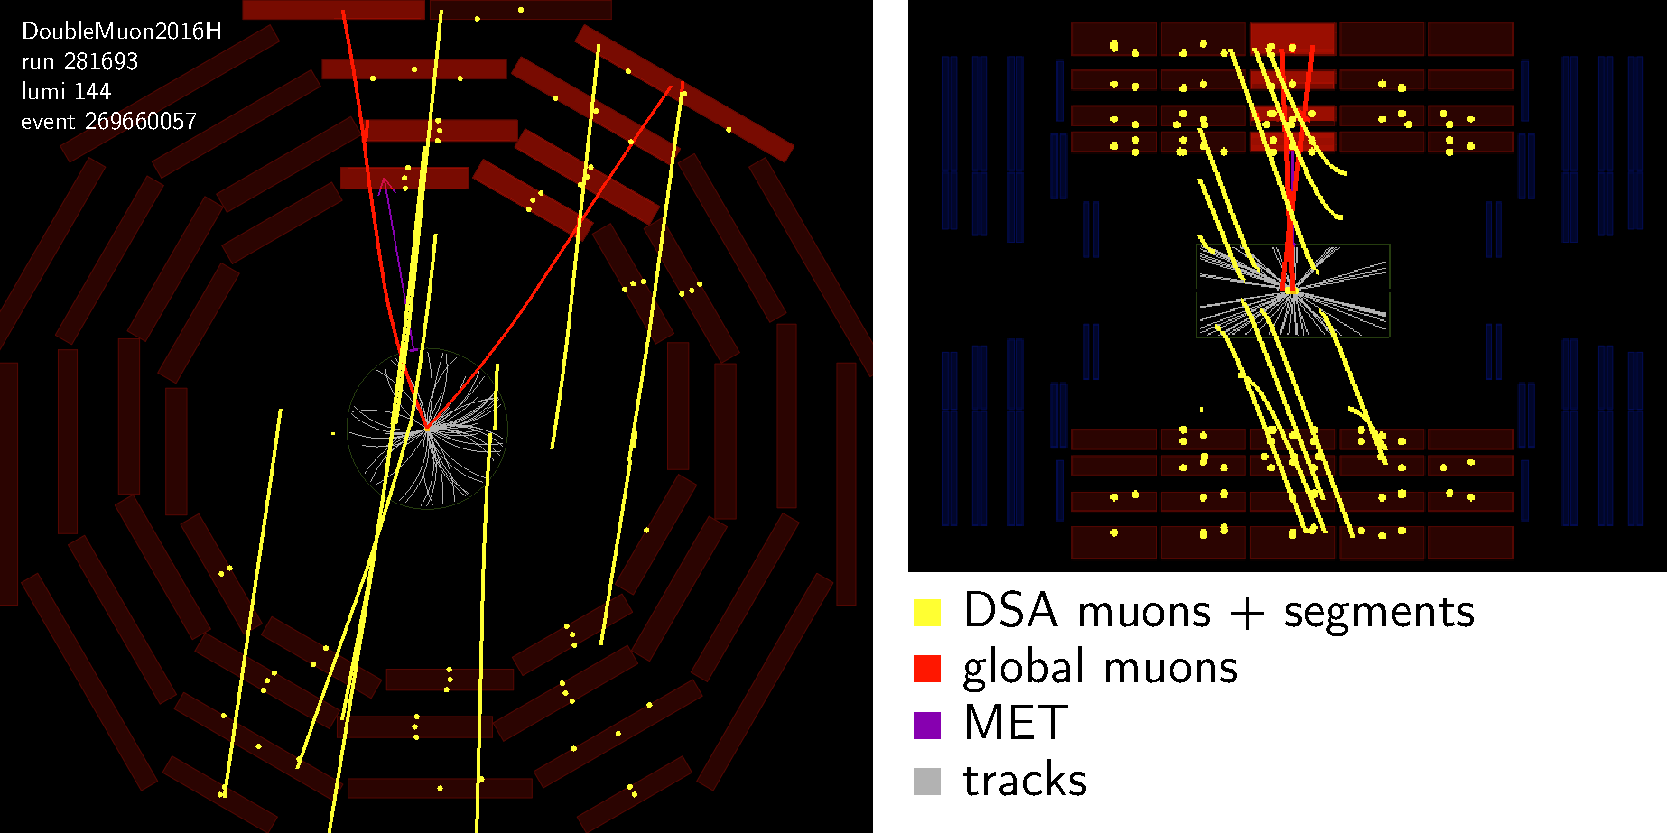
\includegraphics[width=\textwidth]{figures/displaced/ED_Cosmic.pdf}
  \caption[Display of an event in data consistent with multiple cosmic muons from a single atmospheric shower in a \pp collision event.]{Display of an event in data consistent with multiple cosmic muons from a single atmospheric shower in a \pp collision event. Two of the many approximately parallel DSA muons (yellow) reconstructed in this event formed a dimuon vertex with a good \vchisq and the event subsequently passed all our other selections. Requirements that events not contain too many parallel pairs of DSA muons and that the opening angle between the two muons not be too close to $\pi$ were found to be effective in suppressing such events.}
  \label{fig:dd:shower}
\end{figure}

A cosmic muon can be reconstructed as two back-to-back muons, one in the upper half of the detector and one in the lower half of the detector.
A reconstructed dimuon could also be formed from half a cosmic muon and a track from the \pp collision.
These dimuons are reconstructed as highly displaced, which is why the muons have such large $d_0$ values.
The common vertex fit discussed above has anomalous behavior at large displacements, so the presence of the flip-by-$\pi$ and small \pT uncertainty anomalies when fitting to muons with large $d_0$ is perhaps not unexpected.
Such events are background events and so the analysis imposes a set of selections designed to large numbers of cosmic muons.

Some of these events have no \pp collision vertices and contain only cosmic muons.
Events are therefore required to contain at least one well-identified vertex with position $(x, y, z)$ satisfying the following requirements:
\pagebreak
\begin{itemize}
  \item At least 4 degrees of freedom when constructing the vertex
  \item $|z| < 24\mm$
  \item $\sqrt{x^2 + y^2} < 2\mm$
\end{itemize}
This set of requirements is referred to in CMS as the \Code{PrimaryVertexFilter}.

A typical strategy to suppress back-to-back cosmic muons is with a selection on $\cos{\alpha}$, and indeed the trigger has just such a cut, roughly equivalent to $\cos{\alpha} > -0.8$.
Following the trigger, our offline analysis selection also requires $\cos{\alpha} > -0.8$, on the opening angles both between the vertex-constrained muons and between the original (before the vertex fit) muons.

However, these two requirements alone are not sufficient to suppress all events consistent with multiple cosmic muons from an atmospheric shower.
As an additional measure to suppress cosmic muons, the analysis rejects events with a large number of parallel pairs of DSA muons.
All possible pairs of DSA muons, with no common vertex fit, are considered, and the number $N(\text{parallel pairs})$ of such pairs with $|\cos{\alpha}| > 0.99$ are counted.
The analysis selection then requires that events contain no more than 5 such pairs, verified to be of negligible efficiency in signal.

In summary, the cosmic muon suppression selections are
\begin{itemize}
  \item Events pass the \Code{PrimaryVertexFilter}
  \item Events have $N(\text{parallel pairs}) < 6$
  \item Dimuons have original and vertex-constrained $\cos{\alpha} > -0.8$
\end{itemize}

\subsection{Summary of Event and Object Selection}
\Tab~\ref{tab:dd:fullsel} summarizes the full event and object selections discussed in this section.
When setting upper limits, the mass cut is further varied as a function of signal model, as explained in \Sec~\ref{sec:dd:cutopt_mass}.
\begin{table}
  \centering
  \begin{tabular}{llll} 
    \hline\hline
    \multicolumn{4}{c}{Event Selection} \\
    \hline
    primary vertex                    & \multicolumn{3}{l}{\Code{PrimaryVertexFilter} passed}       \\
    HLT-RECO matching                 & \multicolumn{3}{l}{HLT-RECO matching algorithm found match} \\
    number of parallel DSA muon pairs & $N$(parallel pairs) & $<$ & 6                               \\
    \hline
    & & \\

    \hline\hline
    \multicolumn{4}{c}{DSA Muon Selection} \\
    \hline
    association with PAT muons         & \multicolumn{3}{l}{DSA muons \emph{not} associated with PAT muons}  \\
    number of CSC and DT stations      & $N$(CSC+DT stations)                      & $>$ & 1               \\
    number of CSC and DT hits          & $N$(CSC+DT hits)                          & $>$ & 12              \\
    number of DT hits for barrel muons & $N(\text{DT hits}\,\vert\,\text{barrel})$ & $>$ & 18              \\
    relative \pT uncertainty           & $\pTErr/\pT$                              & $<$ & 1               \\
    transverse muon momentum           & \pT                                       & $>$ & 10\GeV          \\
    normalized track \normchisq        & $\chisq_\text{track}/\text{dof}$          & $<$ & 2.5             \\
    time at interaction point          & $|t_\text{in-out}|$                       & $<$ & 12\unit{ns}     \\
    \hline
    & & \\

    \hline\hline
    \multicolumn{4}{c}{Dimuon Selection} \\
    \hline
    distance of closest approach of muon & DCA                            & $<$ & 50\cm          \\
    common vertex fit                    & \multicolumn{3}{l}{common vertex fit converged}       \\
    pairing criteria                     & \multicolumn{3}{l}{best 1--2 ranked dimuons selected} \\
    dimuon mass                          & $\mMuMu$                       & $>$ & 10\GeV*        \\
    vertex \chisq                        & $\chisq_\text{vertex}$         & $<$ & 20             \\
    cosine of dimuon 3D opening angle    & $\cos{\alpha}$                 & $>$ & $-0.8$         \\
    \Lxy significance                    & \LxySig                        & $>$ & 6              \\
    transverse collinearity angle        & \DeltaPhi                      & $<$ & $\pi/4$        \\
    opposite sign muons                  & \multicolumn{3}{l}{constituent muons are oppositely charged} \\
    \hline
  \end{tabular}
  \caption[Summary of full selection, organized into event, muon, and dimuon requirements.]{Summary of full selection, organized into event, muon, and dimuon requirements. The asterisk refers to a selection that varies depending on the signal model used; see \Sec~\ref{sec:dd:cutopt_mass}.}
  \label{tab:dd:fullsel}
\end{table}

\section{Background Estimation}
\label{sec:dd:bgest}
As mentioned above, due to MC simulation limitations, evaluating the expected background in the selection is performed using events in data.
To avoid potential bias while optimizing the analysis, the events passing the full selection in data (the signal region) were blinded until the last steps of the analysis, and the background was estimated using the numbers of events in data in several control regions, which are selections (in the parameter space of the analysis quantities) of subsets of events that are expected to be free of signal events.

As discussed in \Sec~\ref{sec:dd:timing}, after unblinding there was a change made to the selection, notably rejection of a clear class of background events with bad timing.
We also realized that same-sign events could be put to better use in quantitative estimates of the opposite-sign background from QCD events, beyond the rough qualitative use that we had foreseen.

One type of control region is defined as an interval of the transverse collinearity angle, \DeltaPhi.
As discussed in \Sec~\ref{sec:dd:keyvars}, the signal and background have different distributions in \DeltaPhi.
For dimuons consistent with the signal hypothesis, the dimuon momentum vector should be consistent with a particle originating from the primary vertex, and so \DeltaPhi is expected to be small, peaking at zero.
\Fig~\ref{fig:dd:deltaPhi_Sig} shows the distribution of \DeltaPhi for \twoMu signal events (all 33 sets of signal parameters combined) passing the full selection (as described in the previous section), except for the \DeltaPhi cut.

\begin{figure}[htpb]
  \centering
  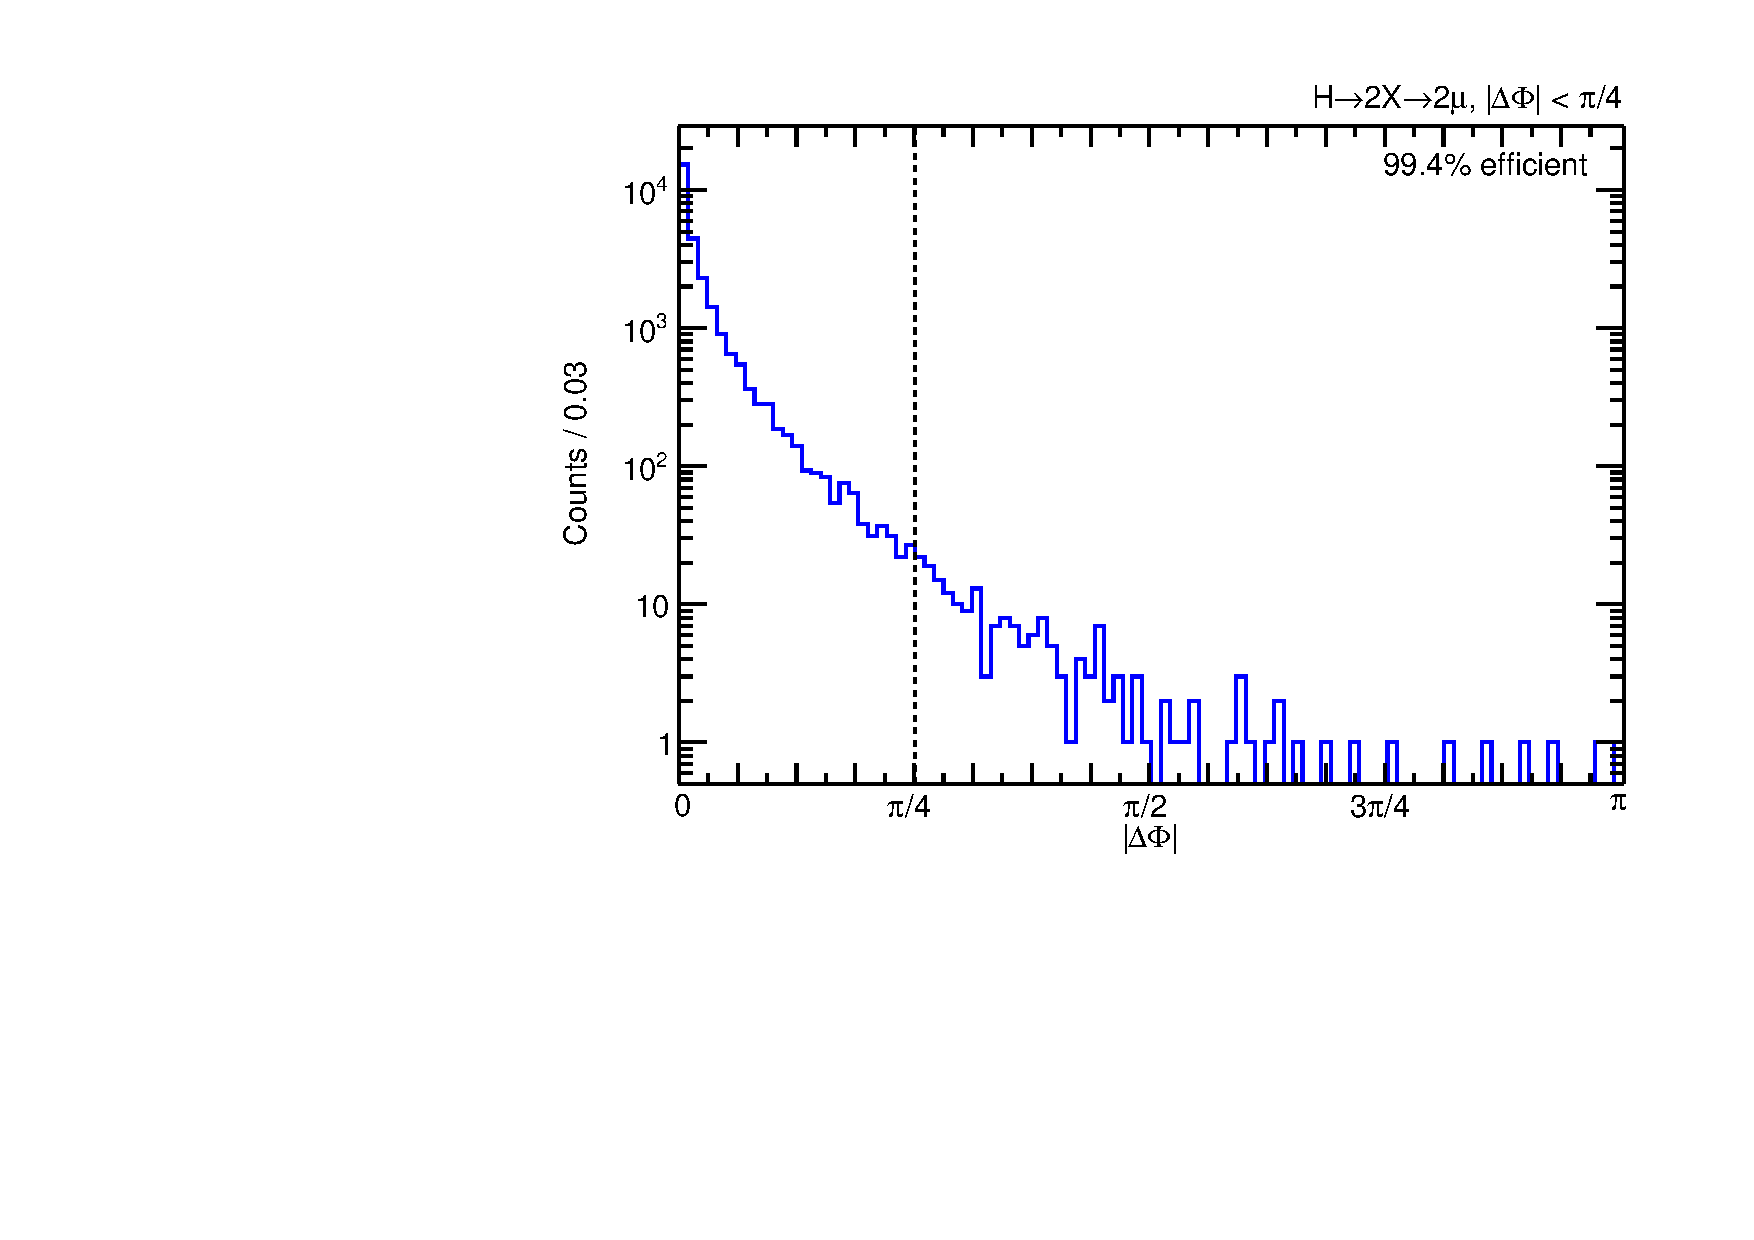
\includegraphics[width=\DFigWidth]{figures/displaced/NM1_2Mu2J_deltaPhi.pdf}
  \caption[Histogram of \DeltaPhi for all \twoMu simulated signal samples combined, showing a strong peak at zero.]{Histogram of \DeltaPhi for all \twoMu signal samples combined, showing a strong peak at zero. The dashed line is at $\DeltaPhi = \pi/4$; the cut $\DeltaPhi < \pi/4$ is 99.4\% efficient in signal.}
  \label{fig:dd:deltaPhi_Sig}
\end{figure}

On the other hand, dimuons in some background events, such as misreconstructed Drell-Yan (DY) events, are expected to have a \DeltaPhi distribution symmetric around $\pi/2$, because the dimuon momentum vector is uncorrelated with the direction of flight from the primary vertex.
This expected symmetry of \DeltaPhi motivates the definition of the signal region as events with \DeltaPhi near 0, \ie $\DeltaPhi < \pi/4$ and a symmetric control region as events with \DeltaPhi near $\pi$, \ie $\DeltaPhi > 3\pi/4$.
A transfer factor (\TF) is defined as the ratio between the number of events in the signal region to the control region.
With $\TF = 1$, the number of events in the control region is a nominal estimate of the expected (Drell-Yan) background in the signal region.

\pagebreak
To validate the approximate background symmetry around $\pi/2$ (and better quantify the transfer factor), the analysis considers pairs of control regions that include the regions $\DeltaPhi < \pi/4$ or $\DeltaPhi > 3\pi/4$ but are formed by reversing other selections (discussed below).

\subsection{Notation for Control Regions}
One set of DSA dimuon control events is obtained by reversal of the \LxySig selection, so that events have small \LxySig instead, \eg $\LxySig < 6$.
Another set of DSA dimuon events are obtained by reversal of the opposite-sign charge selection, so that dimuons consist of muons reconstructed with the same sign.

A final set of DSA dimuon events are obtained by reversal of \DSAToPAT association.
This set consists of DSA dimuons (formed from two DSA muons), passing all selections except for the \DSAToPAT association procedure, in which the two constituent DSA muons can be associated with two PAT muons, and the resulting dimuon formed from two PAT muons has its own PAT \LxySig satisfying a certain range.

Two such ranges are used in this section.
In the first, the PAT \LxySig is small, \eg $\LxySig < 1$.
This region is designed to study Drell-Yan background, and corresponds to DSA dimuons whose PAT muon counterparts are consistent with being produced promptly (and thus are not signal), but which may be reconstructed as highly displaced due to reconstruction mistakes or vertex fit anomalies.
In order to minimize contamination from QCD events, each constituent muon is required to be isolated.
The relative isolation of a muon track is defined as the scalar sum of the \pT of tracks in a \DeltaR cone around the muon divided by the muon \pT.
For this first range, the relative isolation of each constituent PAT muon is required to be at most 0.05.

In the second range, the PAT \LxySig is large, such as \mbox{$60 < \LxySig < 115$}.
This region is designed to study QCD background, such as from cascade decays of $b$ to $c$ quarks or hadrons in flight.
In order to minimize signal contamination, each constituent PAT muon is required to \emph{not} to be isolated, meaning the relative isolation of each constituent PAT muon is required to be at least 0.5.
Less than 3\% of \twoMu signal events satisfy this non-isolation requirement, which meanwhile selects a subset of events composed of approximately 95\% events from QCD processes (according to MC simulation).

With any combination of these three reversals, a pair of control regions may be formed satisfying $\DeltaPhi < \pi/4$ or $\DeltaPhi > 3\pi/4$, respectively.

Some tedious notation is introduced to facilitate discussion of the various control regions.
These regions are labeled CR with the following sublabels:
\begin{itemize}
  \item The superscript on the left side of CR is either 0, 1, 2, or $\pi$, corresponding respectively to the \DeltaPhi ranges $0 < \DeltaPhi < \pi/4$, $\pi/4 < \DeltaPhi < \pi/2$, $\pi/2 < \DeltaPhi < 3\pi/4$, and $3\pi/4 < \DeltaPhi < \pi$.
  \item The subscript on the left side of CR is either OS or SS, corresponding respectively to DSA dimuons consisting of muons with charges of \textbf{o}pposite \textbf{s}ign and muons with charges of the \textbf{s}ame \textbf{s}ign.
  \item The superscript on the right side of CR is of the format $L<x$ or $L>x$ with $x$ a cut value, usually 6, corresponding to DSA dimuons with a reversed \LxySig selection, as described above. This label means that \LxySig value for the dimuon formed from two DSA muons is less than $x$ or greater than $x$. The $L$ in this expression is a reminder that the cut value is for \LxySig.
  \item The subscript on the right side of CR is one of
    \begin{itemize}
      \item $\mathrm{full}$, corresponding to a control region in which the full, standard \DSAToPAT association is performed;
      \item $\mathrm{DY}$, corresponding to the DSA dimuons with reversed \DSAToPAT association as described above with the PAT dimuon satisfying $\LxySig < 1$ and muons isolated; or
      \item $\mathrm{QCD}$, corresponding to the DSA dimuons with reversed \DSAToPAT association as described above with the PAT dimuon satisfying $60 < \LxySig < 115$ and muons not isolated.
    \end{itemize}
    The DSA dimuon passes the selections on \DeltaPhi and \LxySig given by the other two labels. The $\mathrm{DY}$ and $\mathrm{QCD}$ in these expressions indicate the type of background that these control regions are designed to help estimate; the PAT \LxySig ranges were chosen accordingly.
\end{itemize}
For example, \CR[OS]{DY}{<6}{\pi} corresponds to opposite-sign DSA dimuons with \mbox{$\DeltaPhi > 3\pi/4$}, DSA $\LxySig < 6$, and reversed \DSAToPAT association with PAT $\LxySig < 1$.
The signal region SR consisting of DSA dimuons passing all selections can be expressed in this notation as $\mathrm{SR} \equiv\, \CR[OS]{\Full}{>6}{0}$.

\subsection{Estimation of Drell-Yan Background}
\label{sec:dd:bgest-DY}
Misreconstructed Drell-Yan events form a large majority of the background in most regions.
\Fig~\ref{fig:dd:BGDeltaPhi_NoPAT} shows distributions of \DeltaPhi in data and in MC simulation for the control regions with \DSAToPAT association reversed, for all ranges of \DeltaPhi.
The left plot is for all values of \LxySig; that is, it contains both \CR{DY}{>6}{} and \CR{DY}{<6}{} for all \DeltaPhi ranges $(0, 1, 2, \pi)$.
The right plot is only for $\LxySig > 6$; that is, it only contains \CR{DY}{>6}{} for all \DeltaPhi ranges.
Without any \LxySig cut, the distribution is somewhat symmetric, with some excess of events at $\pi$ compared to 0.
With the \LxySig cut, events at 0, $\pi/2$, and $\pi$ are suppressed less than other events, although the distributions are still fairly symmetric.

\begin{figure}[t]
  \centering
  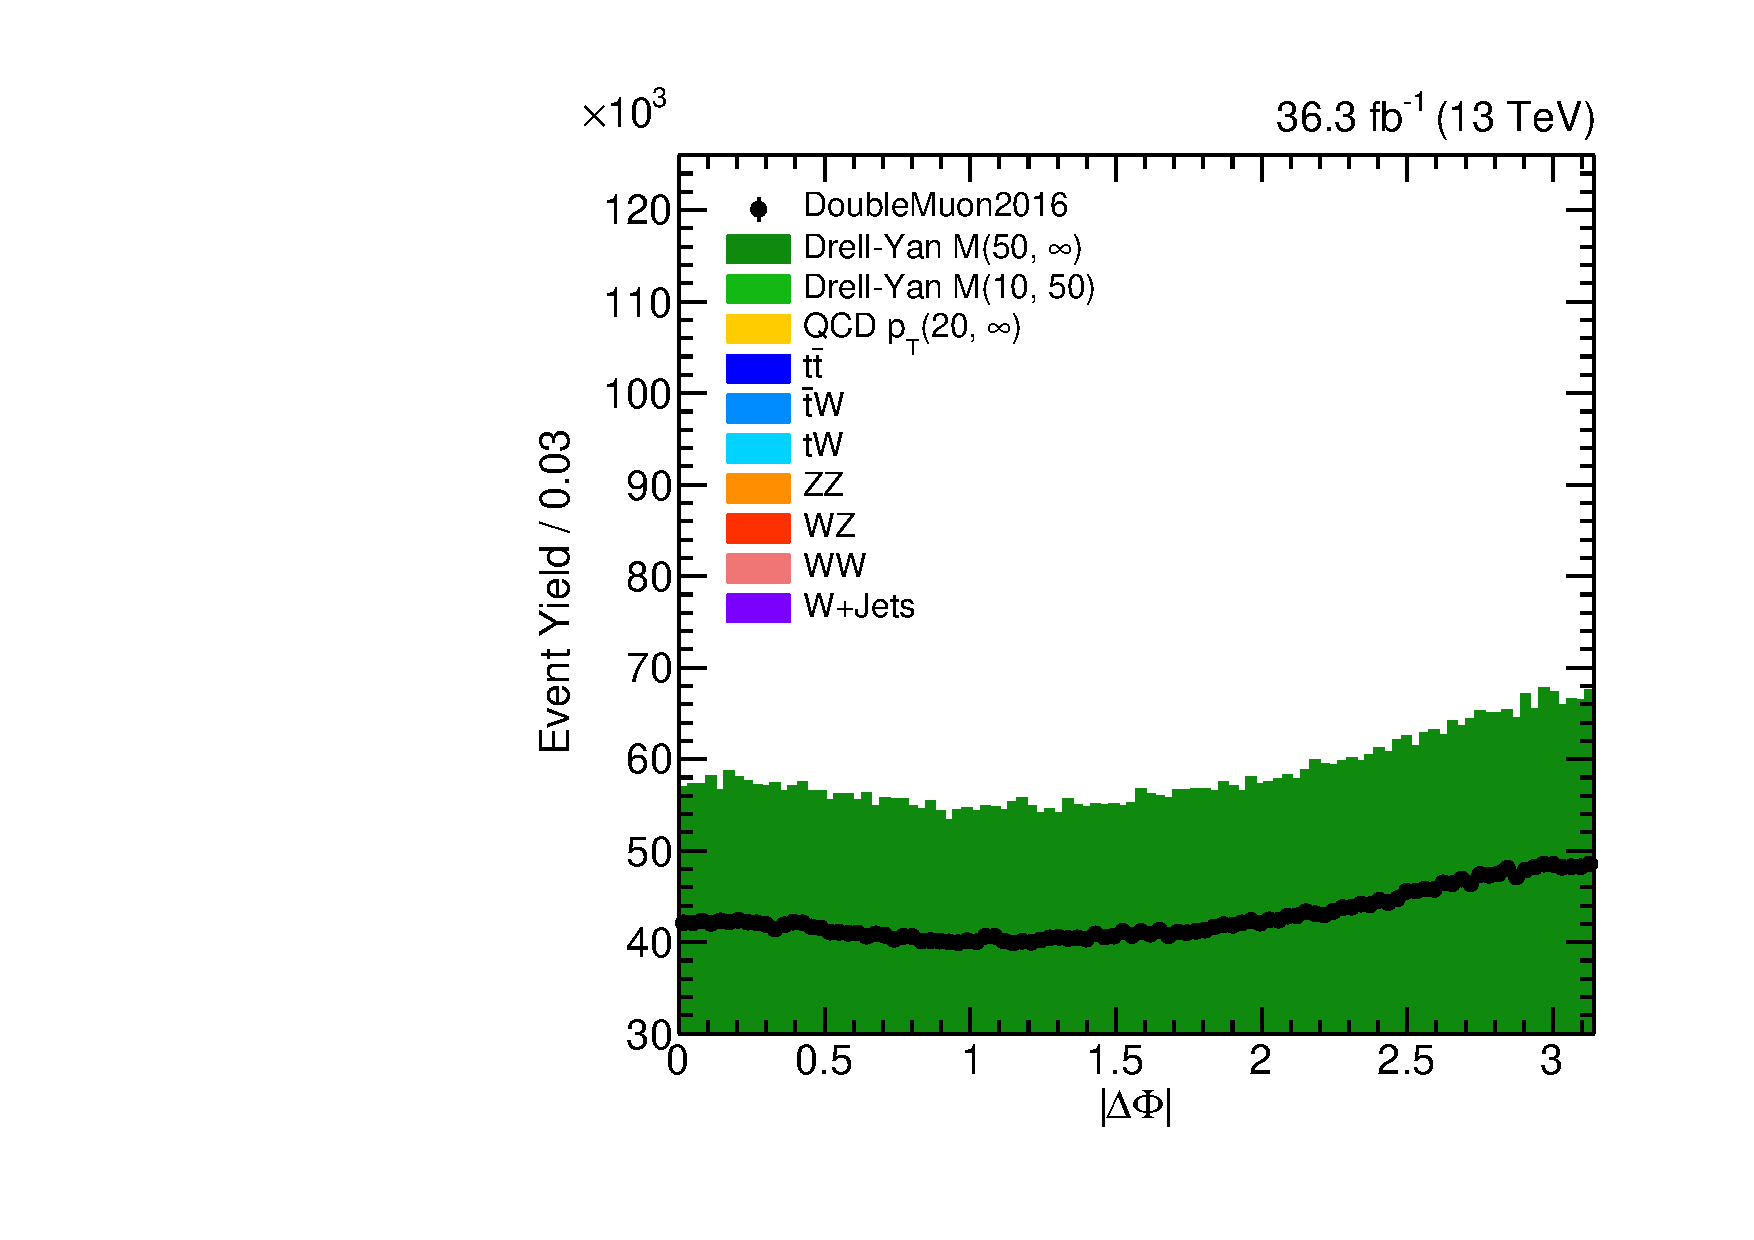
\includegraphics[width=\DSquareWidth]{figures/displaced/BGEST_NOPAT_deltaPhi_Lin.pdf}
  \hspace*{-2em}
  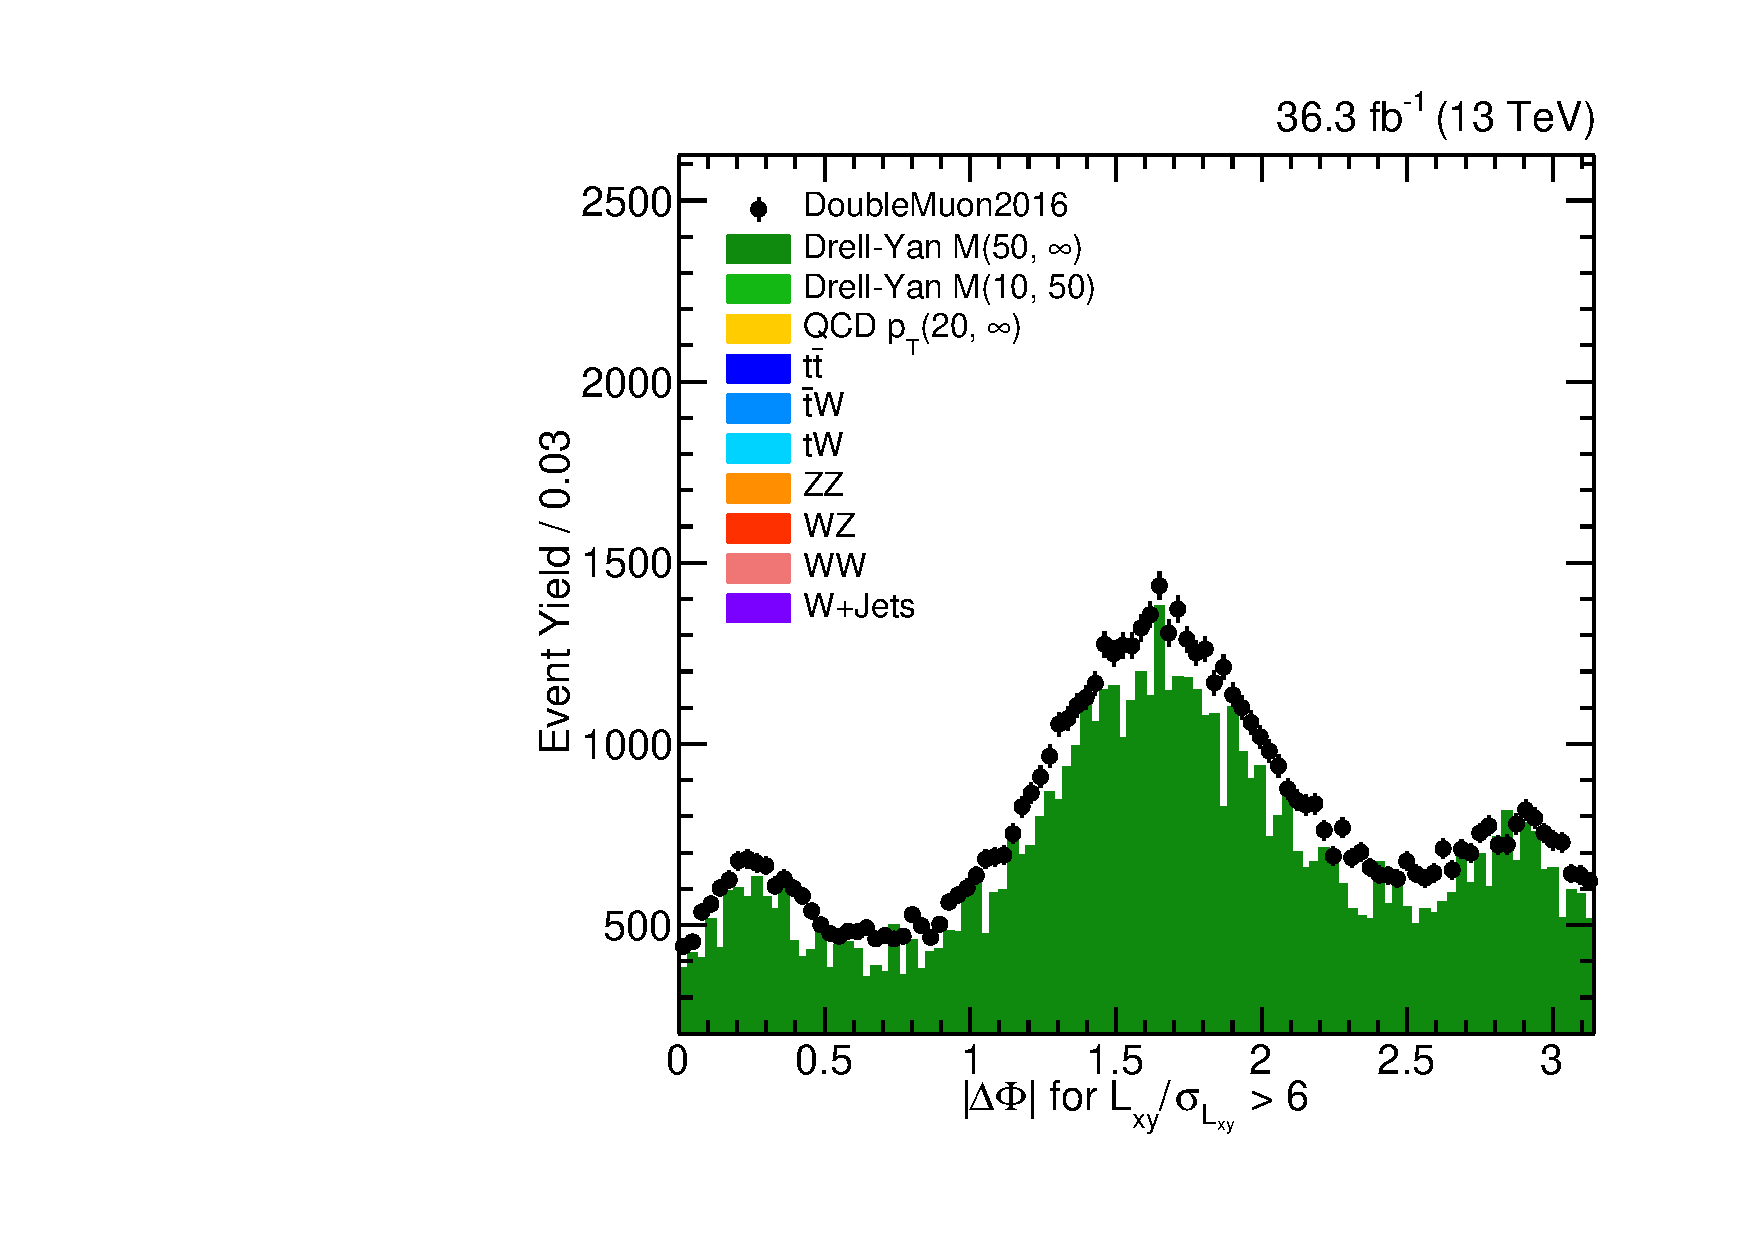
\includegraphics[width=\DSquareWidth]{figures/displaced/BGEST_NOPAT_deltaPhi-Big_Lin.pdf}
  \caption[Histograms of \DeltaPhi in data and in MC simulation for the control regions with \DSAToPAT association reversed, for all values of \DeltaPhi, for all values of \LxySig and for $\LxySig > 6$.]{Histograms of \DeltaPhi in data and in MC simulation for the control regions with \DSAToPAT association reversed, for all values of \DeltaPhi, for \figpos{left} all values of \LxySig and \figpos{right} only $\LxySig > 6$. In the previously introduced notation, \figpos{right} consists of \CR{DY}{>6}{0}, \CR{DY}{>6}{\pi}, \etc, and \figpos{left} consists of all the events in the right plot plus \CR{DY}{<6}{0}, \CR{DY}{<6}{\pi}, \etc Without any \LxySig cut, the distribution is somewhat symmetric, with some excess of events at $\pi$ compared to 0. With the \LxySig cut, events at 0, $\pi/2$, and $\pi$ are suppressed less than other events, although the distributions are still fairly symmetric.}
  \label{fig:dd:BGDeltaPhi_NoPAT}
\end{figure}

Understanding this shape begins by considering Drell-Yan events, which compose a majority of the background, and for which the event geometry often consists of two back-to-back muons.
These muons' directions are often well reconstructed, whereas their \pT may not be, resulting in the dimuon \pT pointing along the direction of one of the muons.
With this event topology in mind, the shape can be explained by the combination of two effects.

The first effect is a result of the decrease in trigger efficiency for large transverse impact parameters $d_{0}$.
Events in which the muon tracks are parallel to the \Lxy vector are events in which the muons point towards the primary vertex, so that their $d_0$ is small.
Events in which the muon tracks are perpendicular to the \Lxy vector are events with large transverse impact parameters, and would be suppressed by the trigger.
But the dimuon \pT is along the direction of one of the muons, so parallel muon tracks correspond to $\DeltaPhi \approx 0$ (or $\pi$), while perpendicular muon tracks correspond to $\DeltaPhi \approx \pi/2$.
In other words, large values of \Lxy only pass the trigger when the muons sufficiently point towards the primary vertex, \ie have $\DeltaPhi \approx 0$ (or $\pi$), effectively suppressing $\DeltaPhi \approx \pi/2$.

(As a thought experiment, consider muons moving in the detector with no magnetic field. Then $d_0 = \Lxy \sin{\DeltaPhi}$.
If the trigger efficiency sharply vanished at some fixed value $d_0 \geq D$, then only events with $\Lxy \leq D \csc{\DeltaPhi}$ would pass the trigger.
Cosecant takes large values around $\DeltaPhi = 0$ and $\DeltaPhi = \pi$, and small values at $\DeltaPhi = \pi/2$.
The diagram in the top row of \Fig~\ref{fig:dd:BGEST_WavyExplanationDiagram} illustrates this first effect in the context of this thought experiment.)

The second effect is a result of geometric effects on the uncertainty of the position of the fitted vertex.
For back-to-back muons, the uncertainty on the fitted dimuon vertex is larger along the direction of the tracks than orthogonal to it, because the uncertainty orthogonal to the track is set by the scatter of hits about the tracks, whereas determining the position of the vertex along two back-to-back tracks is more difficult.
Then for a given \Lxy, the uncertainty on \Lxy, \LxyErr, is larger when the muons (and hence the dimuon \pT) are parallel to the \Lxy vector (\ie $\DeltaPhi = 0$ or $\pi$) and smaller when the muons (and hence the dimuon \pT) are perpendicular to the \Lxy vector (\ie $\DeltaPhi = \pi/2$).
In other words, \LxyErr is smaller at $\pi/2$ than at 0 or $\pi$.
The diagrams in the bottom row of \Fig~\ref{fig:dd:BGEST_WavyExplanationDiagram} illustrate this second effect.

\begin{figure}[htpb]
  \centering
  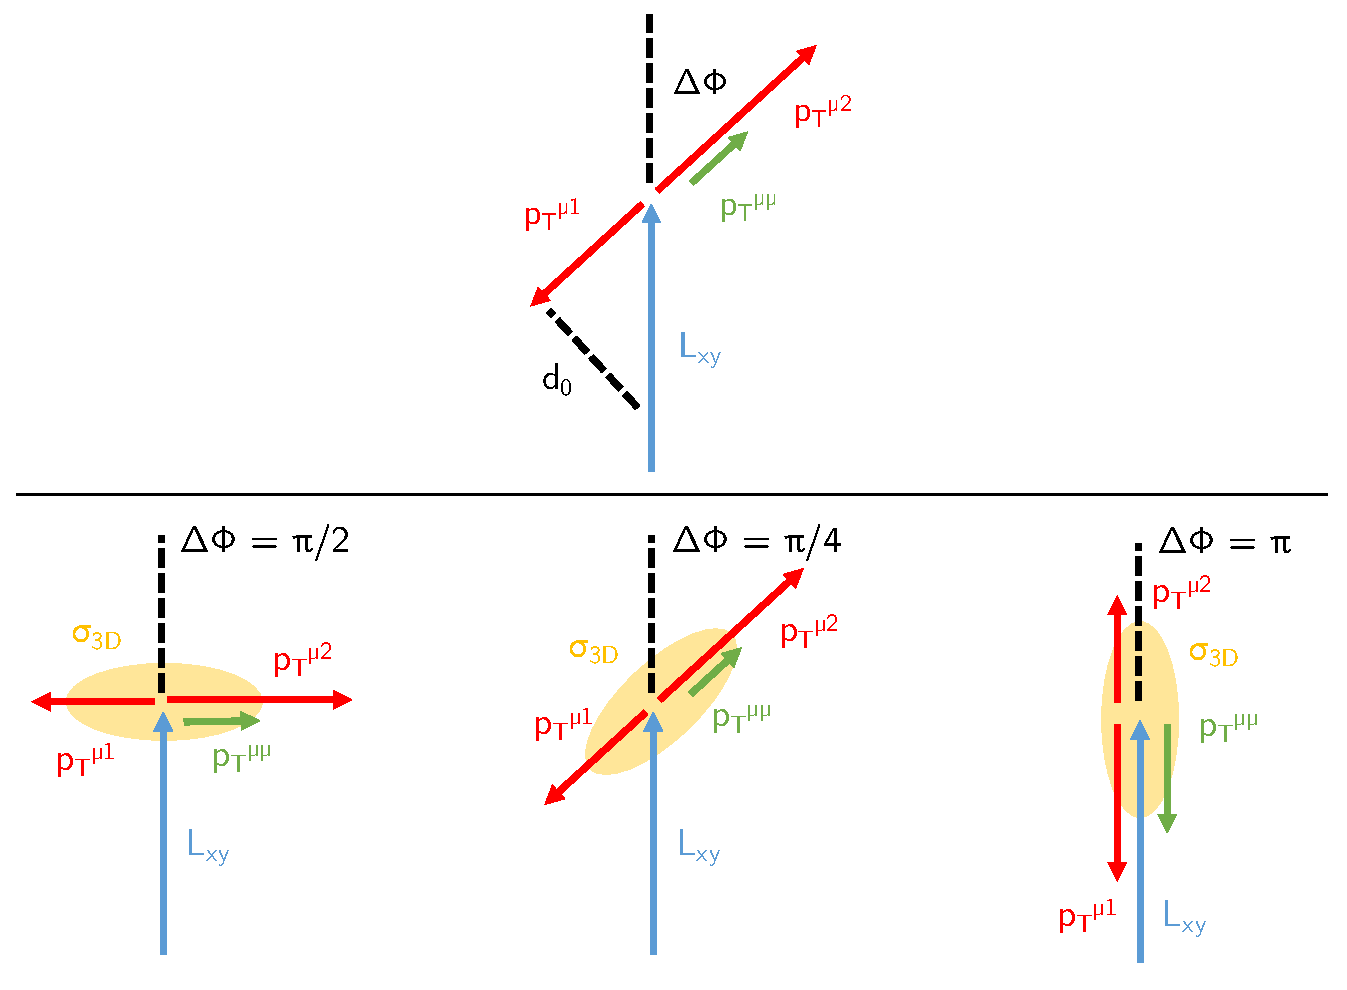
\includegraphics[width=1.2\DFigWidth]{figures/displaced/BGEST_WavyExplanationDiagram.pdf}
  \caption[Diagrams depicting the effect of dimuon orientation on possible values of \Lxy and \LxyErr.]{\figpos{Top} Diagram depicting the effect of dimuon orientation on possible values of \Lxy. Lowered trigger efficiency at large transverse impact parameter ($d_0$) values suppresses large \Lxy values, which have significant $d_0$ unless \DeltaPhi is sufficiently close to 0 or $\pi$. \figpos{Bottom} Diagram depicting the effect of dimuon orientation on \LxyErr as a function of \DeltaPhi. The dimuon \pT points along one of the muons, which are back-to-back, and the uncertainty on the position of the fitted vertex is represented by a yellow ellipse around the vertex, with the larger axis parallel to the muon. For a given \Lxy the \LxyErr is larger when the muons are parallel to the \Lxy vector (\ie $\DeltaPhi = 0$ or $\pi$) and smaller when the muons are perpendicular to it (\ie $\DeltaPhi = \pi/2$), taking an intermediate value with $\DeltaPhi = \pi/4$ (or $3\pi/4$).}
  \label{fig:dd:BGEST_WavyExplanationDiagram}
\end{figure}

A selection on \LxySig selects events with large \Lxy and/or small \LxyErr, which have been shown to preferentially occur at 0, $\pi/2$, and $\pi$.
The resulting shape of the \DeltaPhi distribution appears to be geometric in origin, and is the motivation for defining the signal and control regions as $\DeltaPhi < \pi/4$ and its symmetric region around $\pi/2$, in order to cut away from the extra background at $\pi/2$.
\Fig~\ref{fig:dd:SeqLxySig} shows the $\DeltaPhi$ distributions as in the right plot of \Fig~\ref{fig:dd:BGDeltaPhi_NoPAT}, each scaled to unit area, for data and for Drell-Yan simulation, for sequentially increasing cuts on \LxySig (\ie \CR{DY}{>x}{} for all \DeltaPhi and $x$ variable).
The Drell-Yan plot indicates that the shape is well-reproduced by simulation.

\begin{figure}[t]
  \centering
  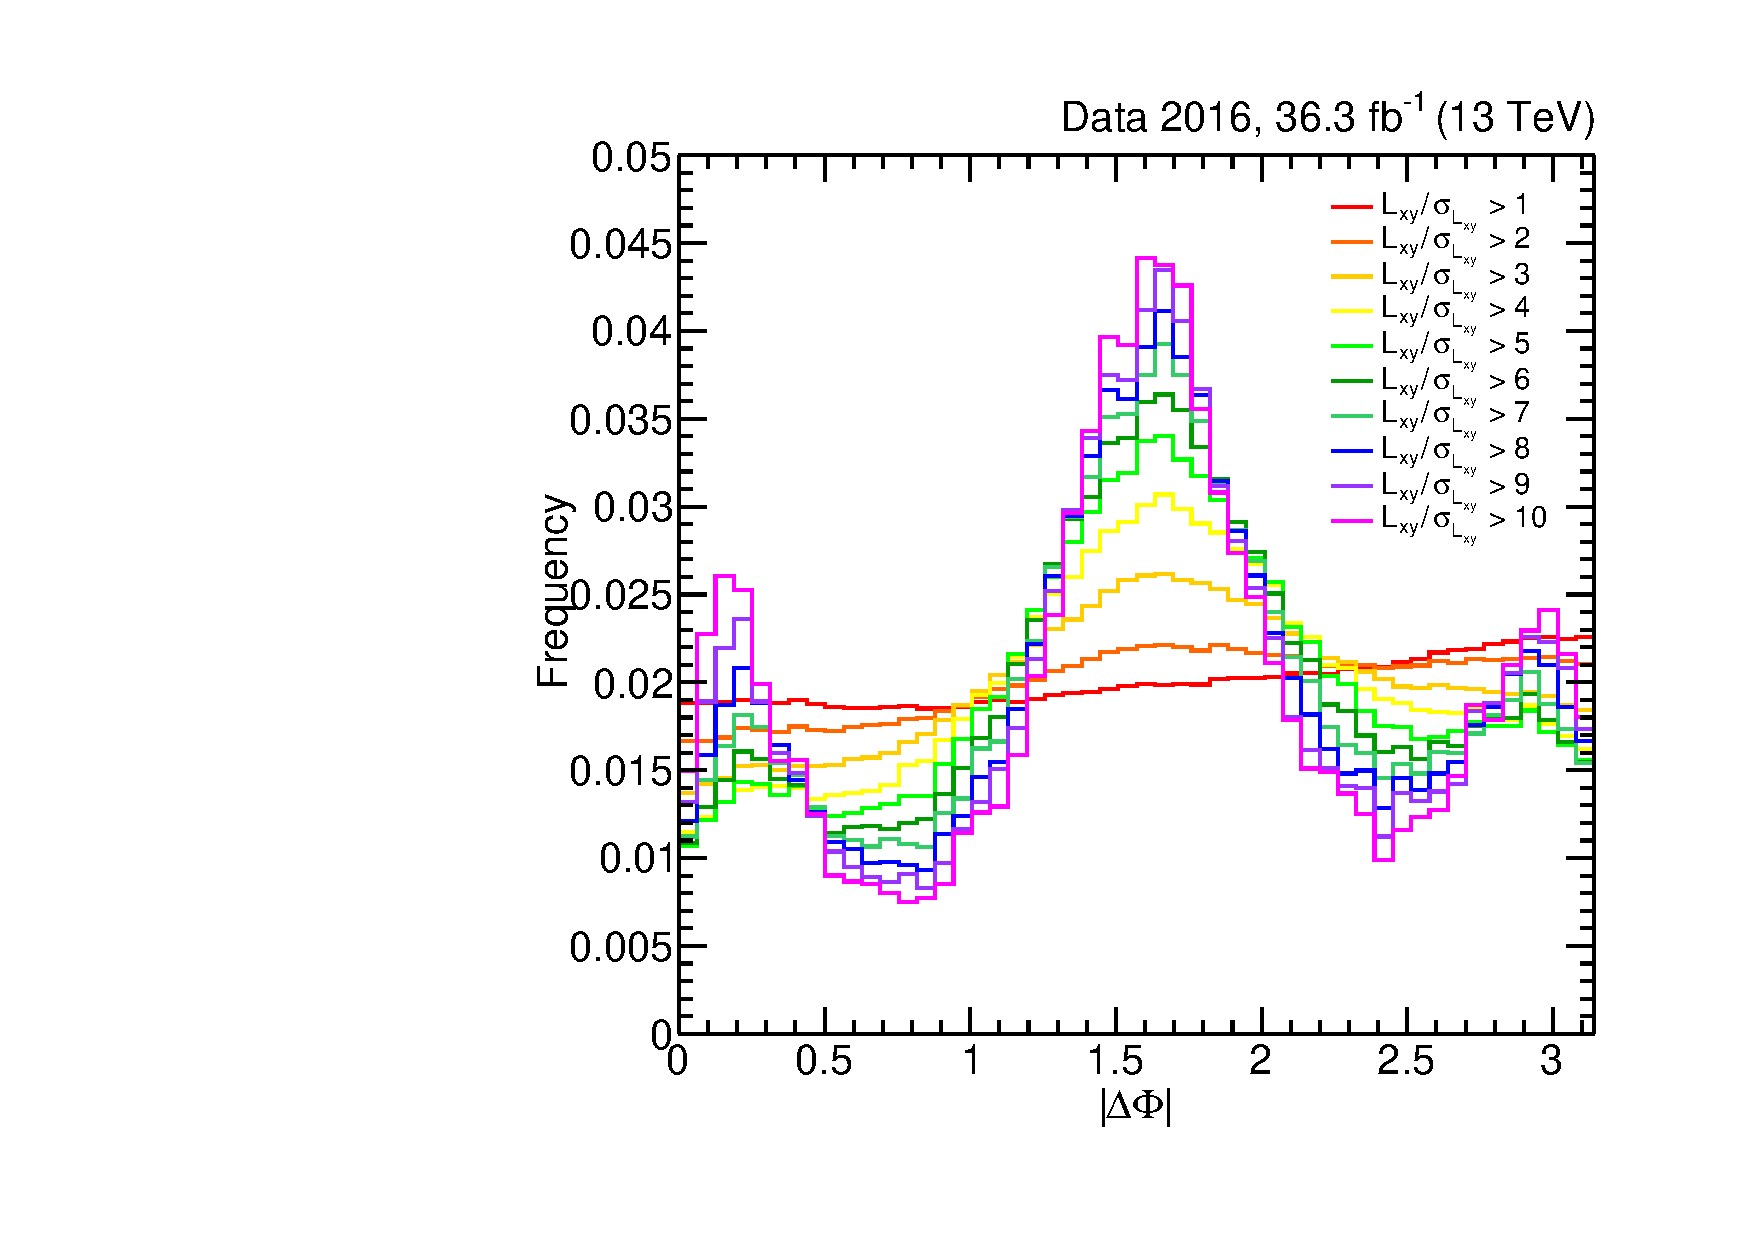
\includegraphics[width=\DSquareWidth]{figures/displaced/BGEST_EffectOfLxySigCut_DeltaPhi_Data_DY-Like.pdf}
  \hspace*{-2em}
  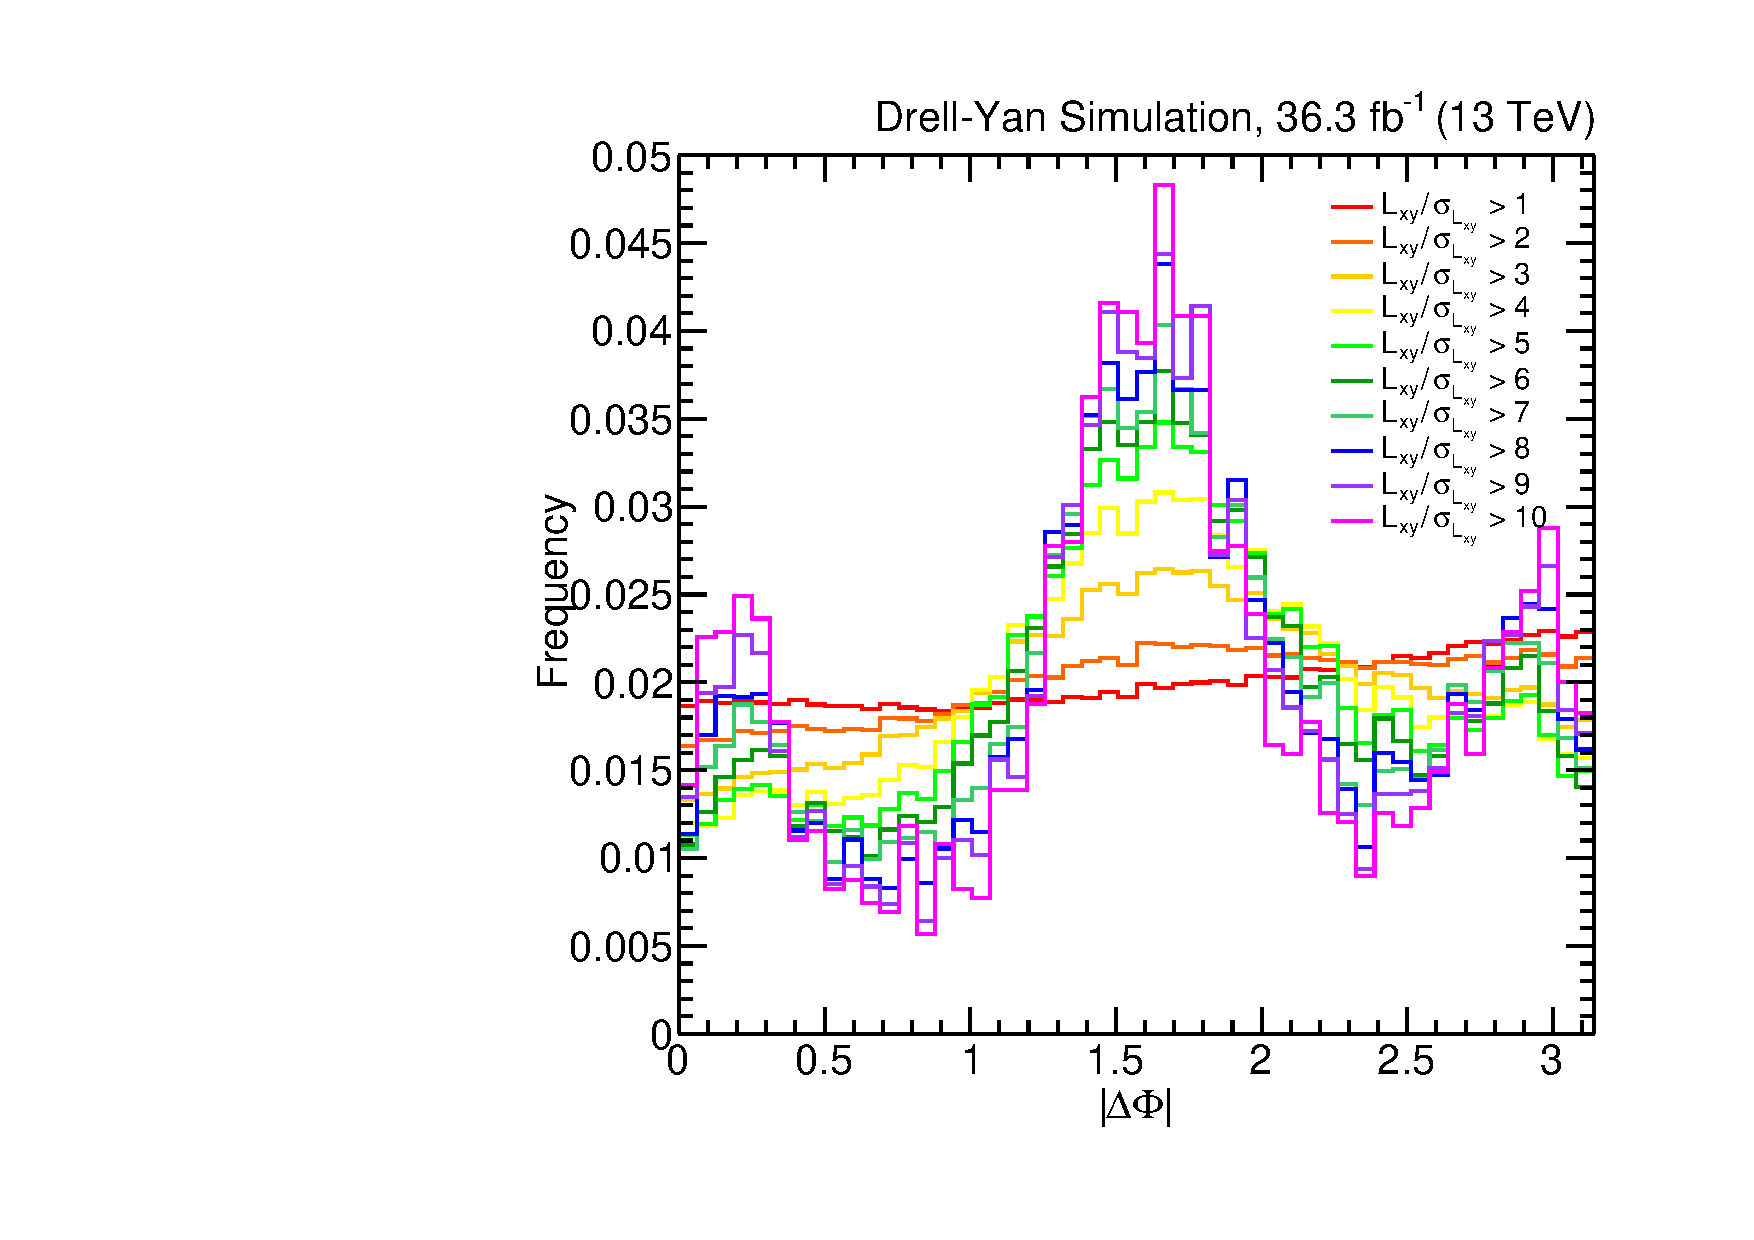
\includegraphics[width=\DSquareWidth]{figures/displaced/BGEST_EffectOfLxySigCut_DeltaPhi_MC_DY-Like.pdf}
  \caption[Histograms of \DeltaPhi for sequentially increasing cut values of \LxySig in data and Drell-Yan simulation.]{Histograms of \DeltaPhi as in \Fig~\ref{fig:dd:BGDeltaPhi_NoPAT}, normalized to unit area, for sequentially increasing cut values of \LxySig for \figpos{left} data and \figpos{right} Drell-Yan simulation.}
  \label{fig:dd:SeqLxySig}
\end{figure}

\begin{table}
  \centering
  \begin{tabular}{lcccl}
    \hline
    Name  & Events \\
    \hline
    SR                  & ?       \\
    \CR{\Full}{>6}{\pi} & 0       \\
    \CR{\Full}{<6}{0}   & 60      \\
    \CR{\Full}{<6}{\pi} & 55      \\
    \CR{DY}   {>6}{0}   & 13636   \\
    \CR{DY}   {>6}{\pi} & 17405   \\
    \CR{DY}   {<6}{0}   & 1026522 \\
    \CR{DY}   {<6}{\pi} & 1153133 \\
    \hline
  \end{tabular}
  \caption[Event counts for control regions for estimating Drell-Yan background.]{Event counts for control regions for estimating Drell-Yan background. The ratio of \CR{DY}{>6}{0} to \CR{DY}{>6}{\pi} gives a transfer factor; multiplying the number of events in \CR{\Full}{>6}{\pi} by this transfer factor gives an estimate of the Drell-Yan background in SR.}
  \label{tab:dd:controlregions}
\end{table}

\Tab~\ref{tab:dd:controlregions} gives the number of events in data for each of the control regions.
A data-driven estimate of the transfer factor $\TF_\text{DY}$ can be obtained by dividing the number of events in \CR{DY}{>6}{0} by the number of events in \CR{DY}{>6}{\pi} and is found to be

\begin{equation}
  \TF_\text{DY} = \frac{N\left[\CR{DY}{>6}{0}\right]}{N\left[\CR{DY}{>6}{\pi}\right]} = 0.78
  \label{eq:dd:DYtransferfactor}
\end{equation}

Other ratios, such as $\CR{DY}{<6}{0}/\CR{DY}{<6}{\pi} = 0.89$ and $\CR{\Full}{<6}{0}/\CR{\Full}{<6}{\pi} = 1.09$ serve to validate the (approximate) symmetry in the Drell-Yan background (because the values are close to 1).

There are 0 events in the full 2016 dataset in \CR{\Full}{>6}{\pi}.
The estimate of the expected Drell-Yan background in SR is therefore also 0 events (with or without the mass window cuts described in \Sec~\ref{sec:dd:cutopt_mass}).
The systematic uncertainty on $\TF_\text{DY}$ is described and evaluated in \Sec~\ref{sec:dd:bgunc}.

\subsection{Estimation of QCD Background}
\label{sec:dd:bgest-QCD}
Background events arising from QCD processes, such as from collimated muons in jets, hadron decays in flight, or cascade decays of $b$ and $c$ quarks, may have large, signal-like \LxySig values and dimuon masses in the range $10\GeV < \mMuMu < 40\GeV$.
\DeltaPhi for such events may not be symmetric around $\pi/2$, instead having a peak at 0.

\Fig~\ref{fig:dd:SeqLxySig_QCD_DeltaPhi} illustrates this with a histogram of \DeltaPhi for opposite sign events with the \DSAToPAT association reversed, with the corresponding matched PAT dimuon satisfying $60 < \LxySig < 115$, and the constituent PAT muon tracks not isolated, for sequentially increasing cuts on DSA \LxySig.
Unlike the DY-like events in the data plot of \Fig~\ref{fig:dd:SeqLxySig}, which are symmetric around $\pi/2$, these events have a strong, signal-like peak in \DeltaPhi at 0, especially for larger values of \LxySig.

\begin{figure}[htpb]
  \centering
  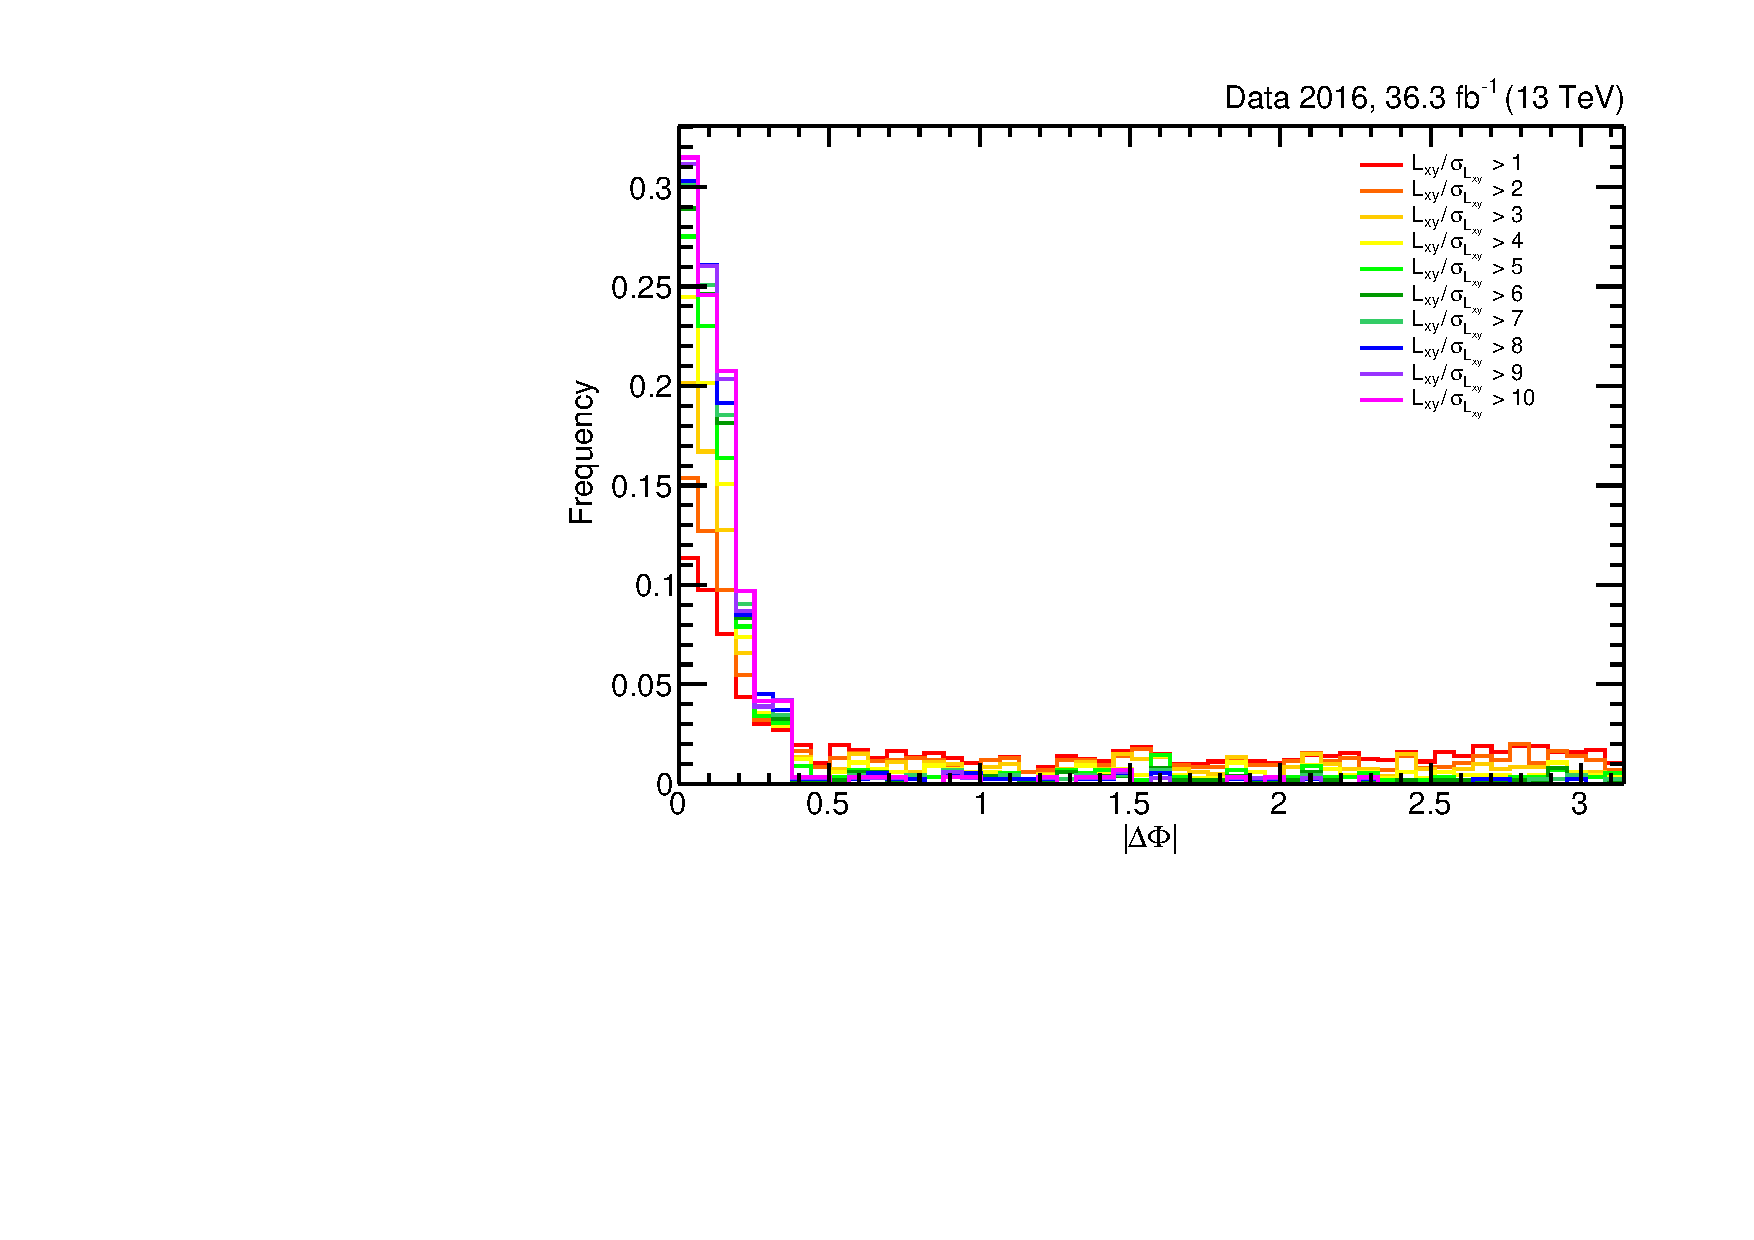
\includegraphics[width=\DFigWidth]{figures/displaced/BGEST_EffectOfLxySigCut_DeltaPhi_Data_QCD-Like.pdf}
  \caption[Histogram of \DeltaPhi for sequentially increasing cut values of \LxySig for QCD-like events in data.]{Histogram of \DeltaPhi for sequentially increasing cut values of \LxySig in data for the control region \CR[OS]{QCD}{>x}{0}, normalized to unit area, with variable, sequentially increasing cut values $x$ of DSA \LxySig. These events are QCD-like, and have a strong, signal-like peak in \DeltaPhi at 0, especially for larger values of \LxySig, in stark contrast to the symmetry around $\pi/2$ of the DY-like events in the data plot of \Fig~\ref{fig:dd:SeqLxySig}.}
  \label{fig:dd:SeqLxySig_QCD_DeltaPhi}
\end{figure}

\pagebreak
To demonstrate that calling these two sets of events DY-like and QCD-like is justified, \Fig~\ref{fig:dd:SeqLxySig_DY_MassDeltaR} shows histograms of \mMuMu and $\deltaR(\Pgm\Pgm)$ for sequentially increasing cut values of \LxySig in data, as in \Fig~\ref{fig:dd:SeqLxySig}, for the events in the control region (\ie \CR{DY}{>x}{0} for variable $x$) used to estimate the Drell-Yan background in \Sec~\ref{sec:dd:bgest-DY}.
As the cut increases, the contribution of the \PZ\ mass peak decreases, and the contribution of QCD events at lower mass increases slightly.
Moreover, the \deltaR distribution is highly DY-like, with a strong peak at $\pi$ whose contribution also decreases with increasing \LxySig cut values, with some enhancement of low \deltaR QCD background.

In contrast, \Fig~\ref{fig:dd:SeqLxySig_QCD_MassDeltaR} shows similar histograms of \mMuMu and $\deltaR(\Pgm\Pgm)$ for the QCD-like events in data (\ie \CR[OS]{QCD}{>x}{0} for variable $x$).
As the cut increases, the contribution of lower mass QCD events increases, and the \deltaR distribution has a strong peak at 0, suggestive of QCD background, with successively decreasing contributions from Drell-Yan backgrounds at $\pi$.

\begin{figure}[p]
  \centering
  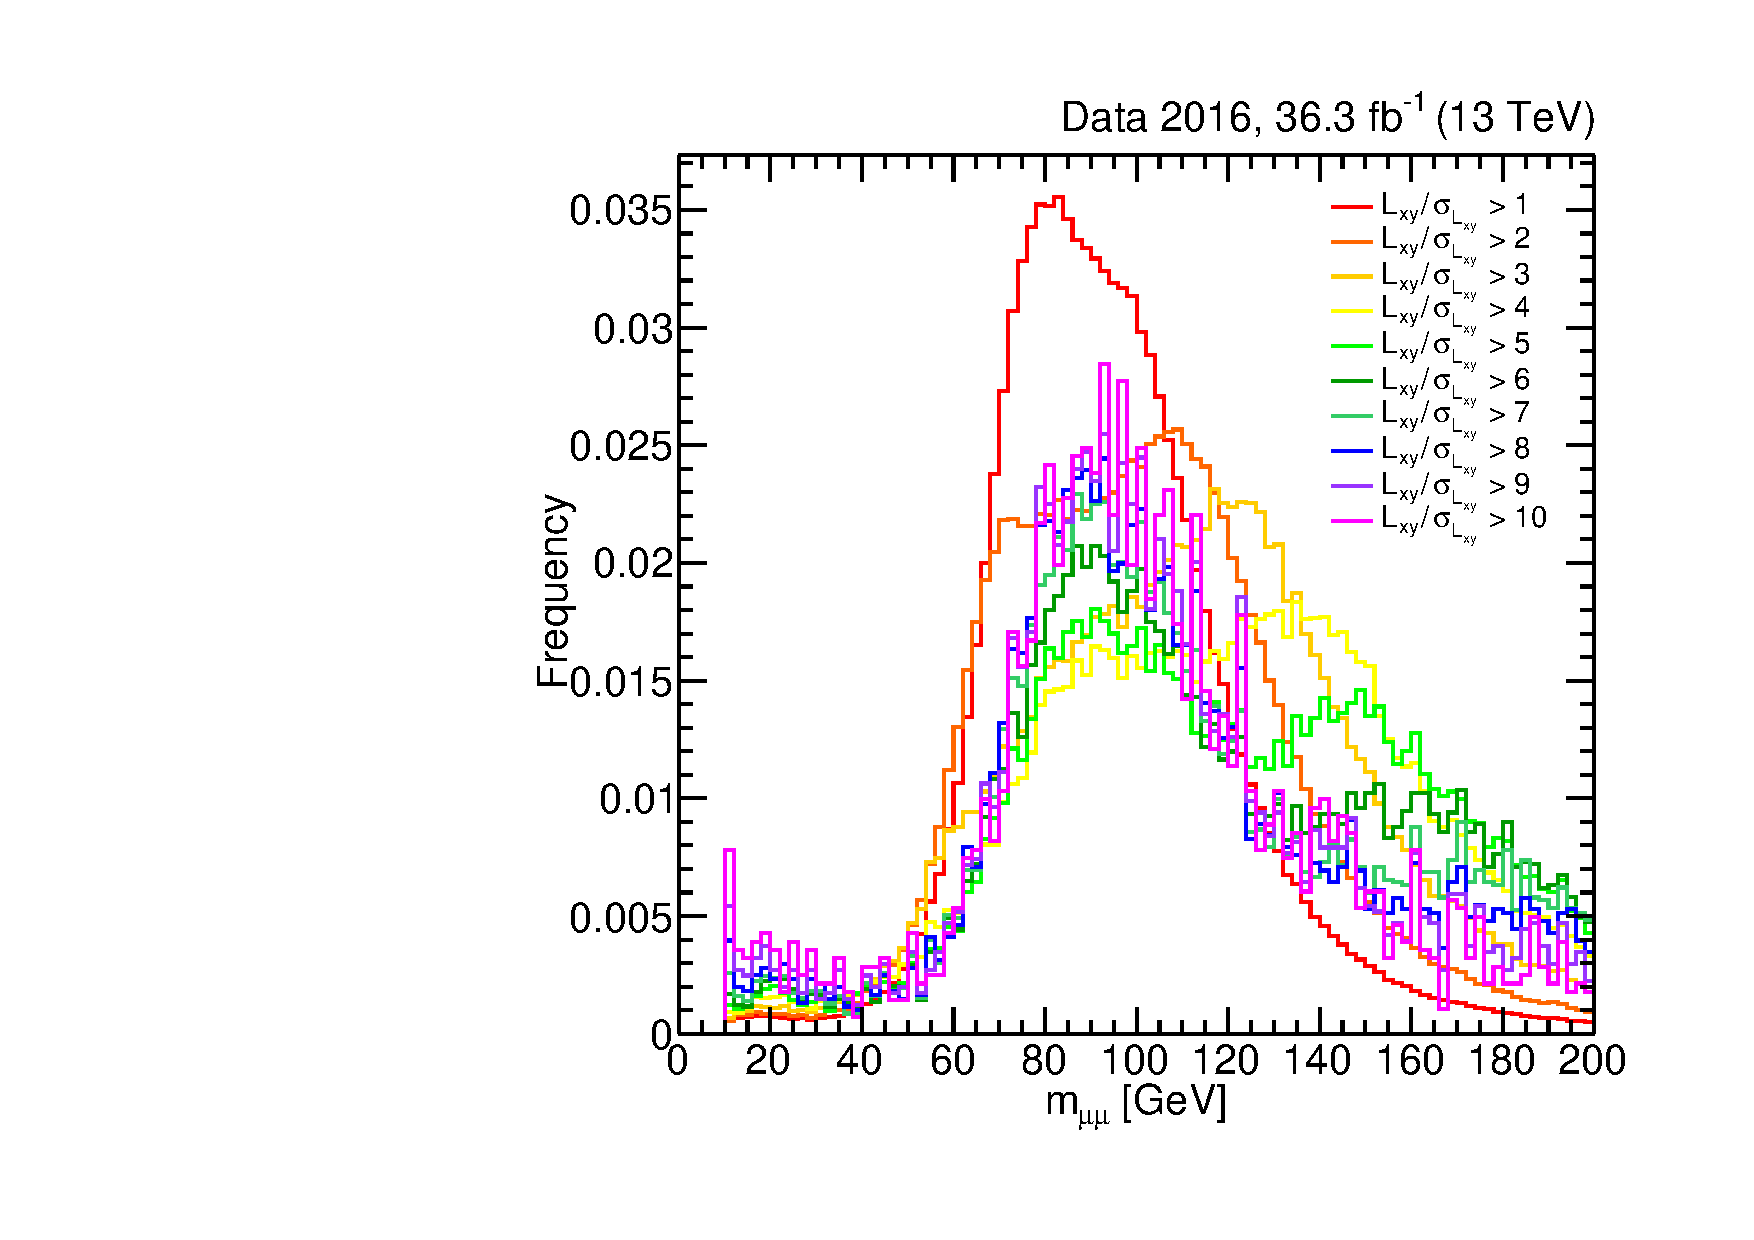
\includegraphics[width=\DSquareWidth]{figures/displaced/BGEST_EffectOfLxySigCut_Mass_Data_DY-Like.pdf}
  \hspace*{-2em}
  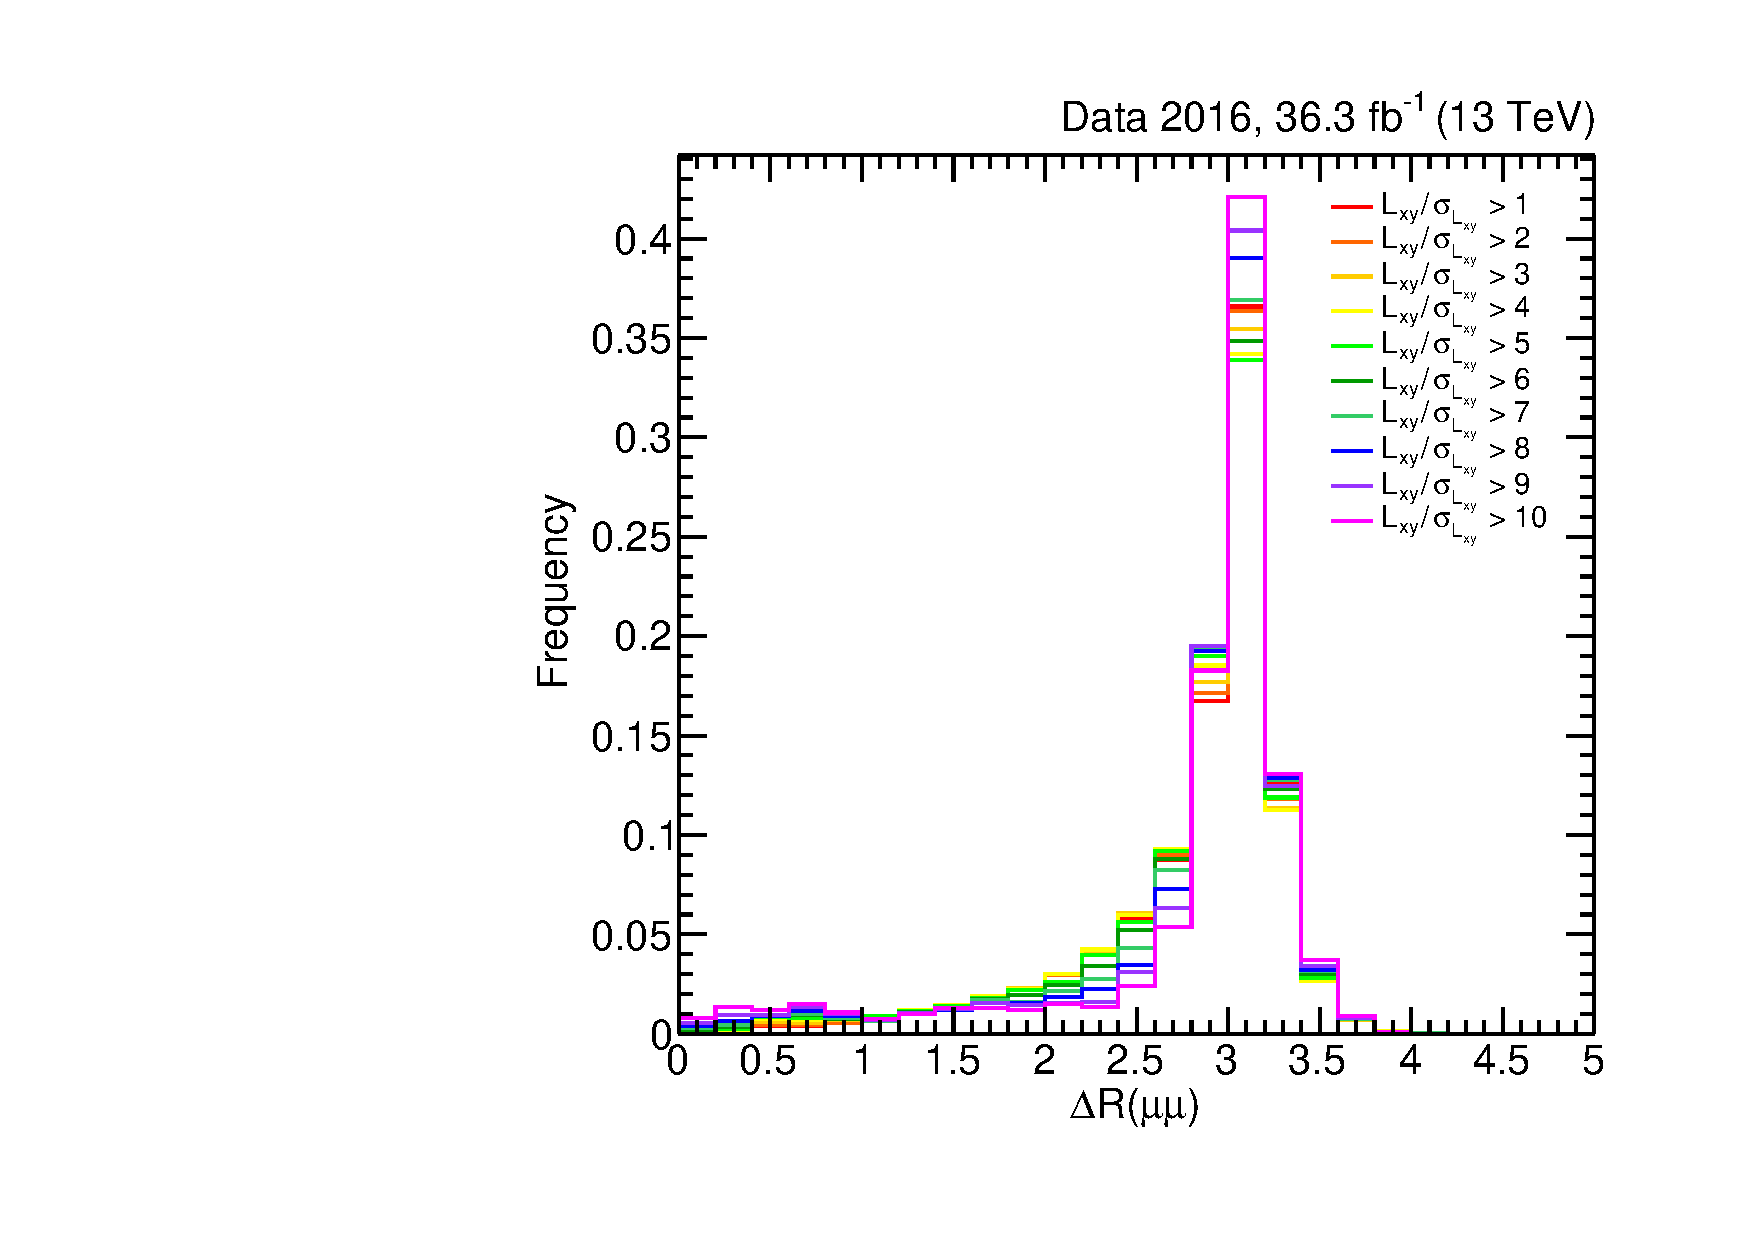
\includegraphics[width=\DSquareWidth]{figures/displaced/BGEST_EffectOfLxySigCut_DeltaR_Data_DY-Like.pdf}
  \caption[Histograms of \mMuMu and $\deltaR(\Pgm\Pgm)$ for DY-like events in data for sequentially increasing cut values of \LxySig.]{Histograms of \figpos{left} \mMuMu and \figpos{right} $\deltaR(\Pgm\Pgm)$ for sequentially increasing cut values of \LxySig in data as in \Fig~\ref{fig:dd:SeqLxySig}, normalized to unit area, using the control regions \CR{DY}{>x}{0} for variable, sequentially increasing cut values $x$ of DSA \LxySig.}
  \label{fig:dd:SeqLxySig_DY_MassDeltaR}
\end{figure}

\begin{figure}[p]
  \centering
  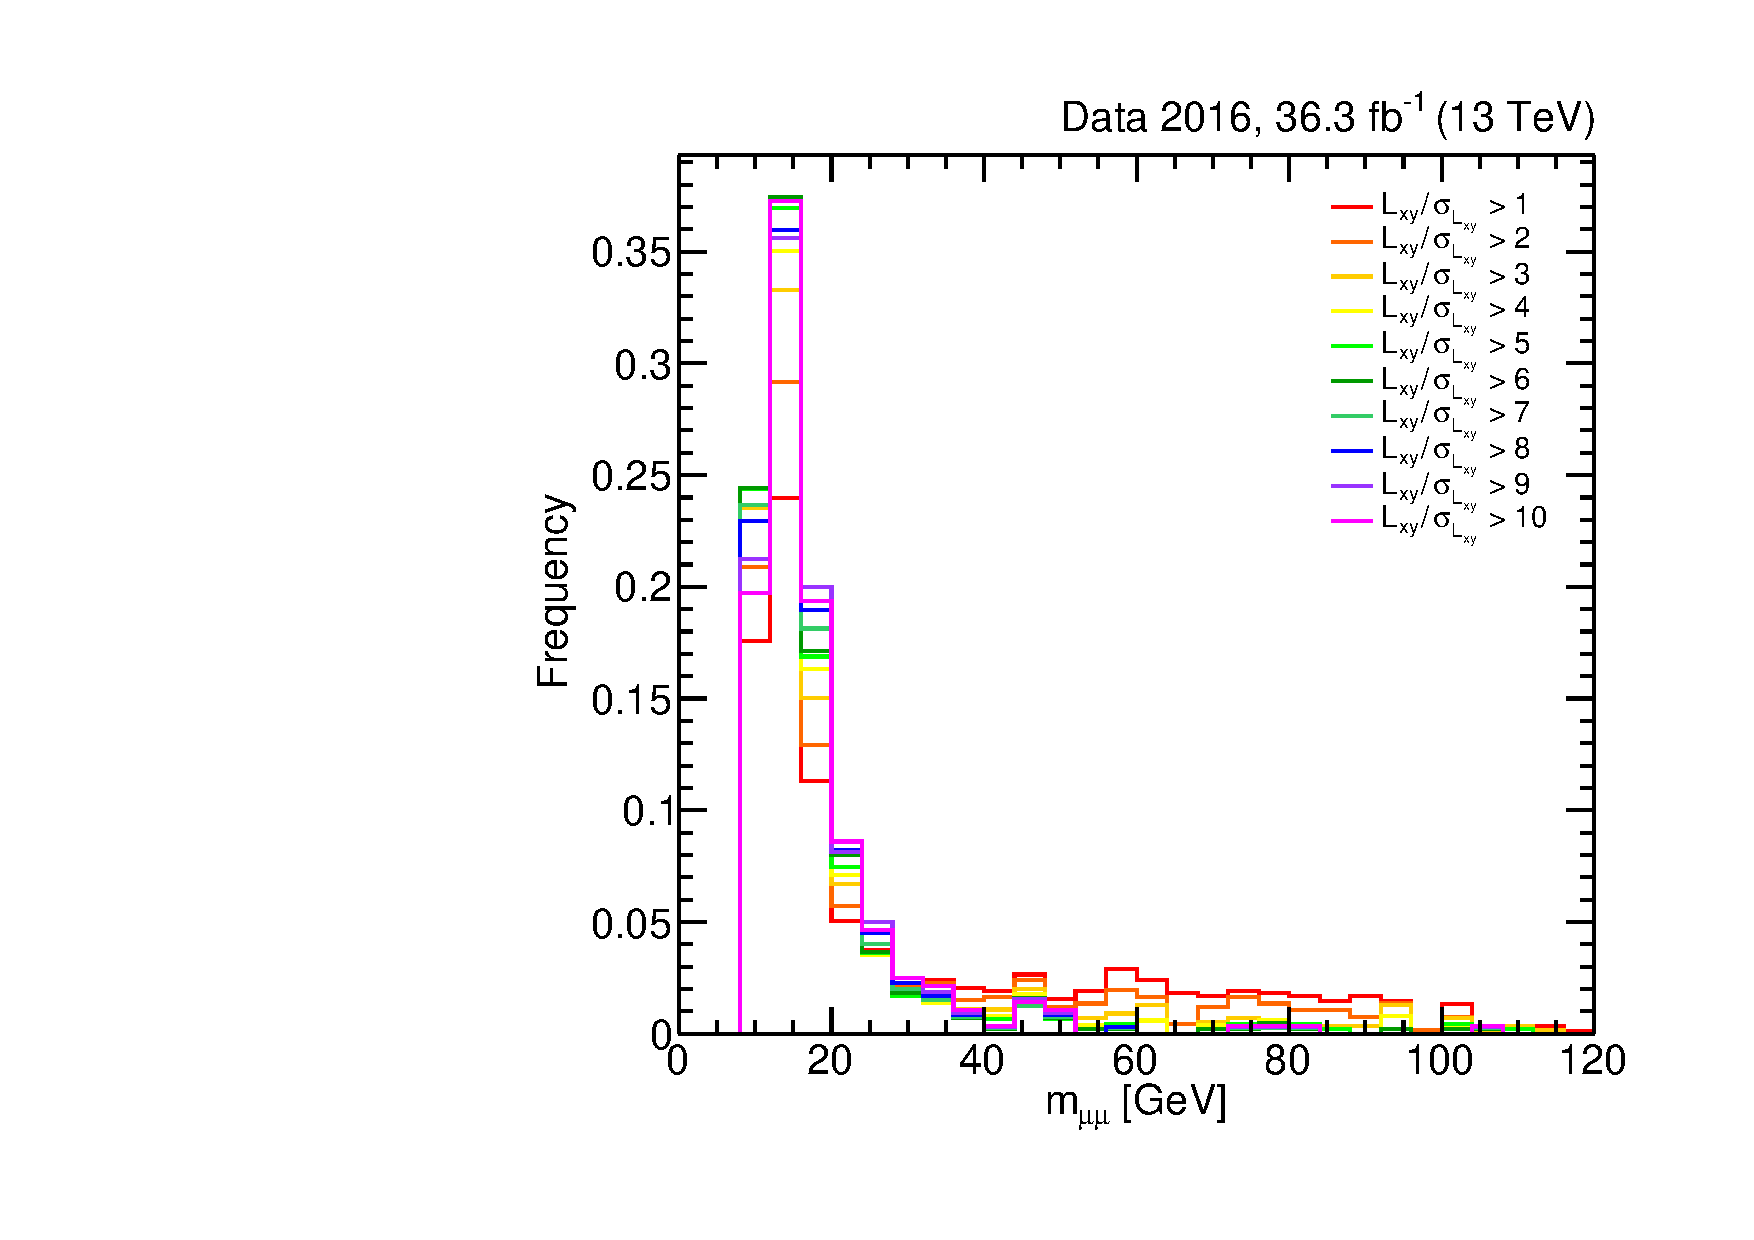
\includegraphics[width=\DSquareWidth]{figures/displaced/BGEST_EffectOfLxySigCut_Mass_Data_QCD-Like.pdf}
  \hspace*{-2em}
  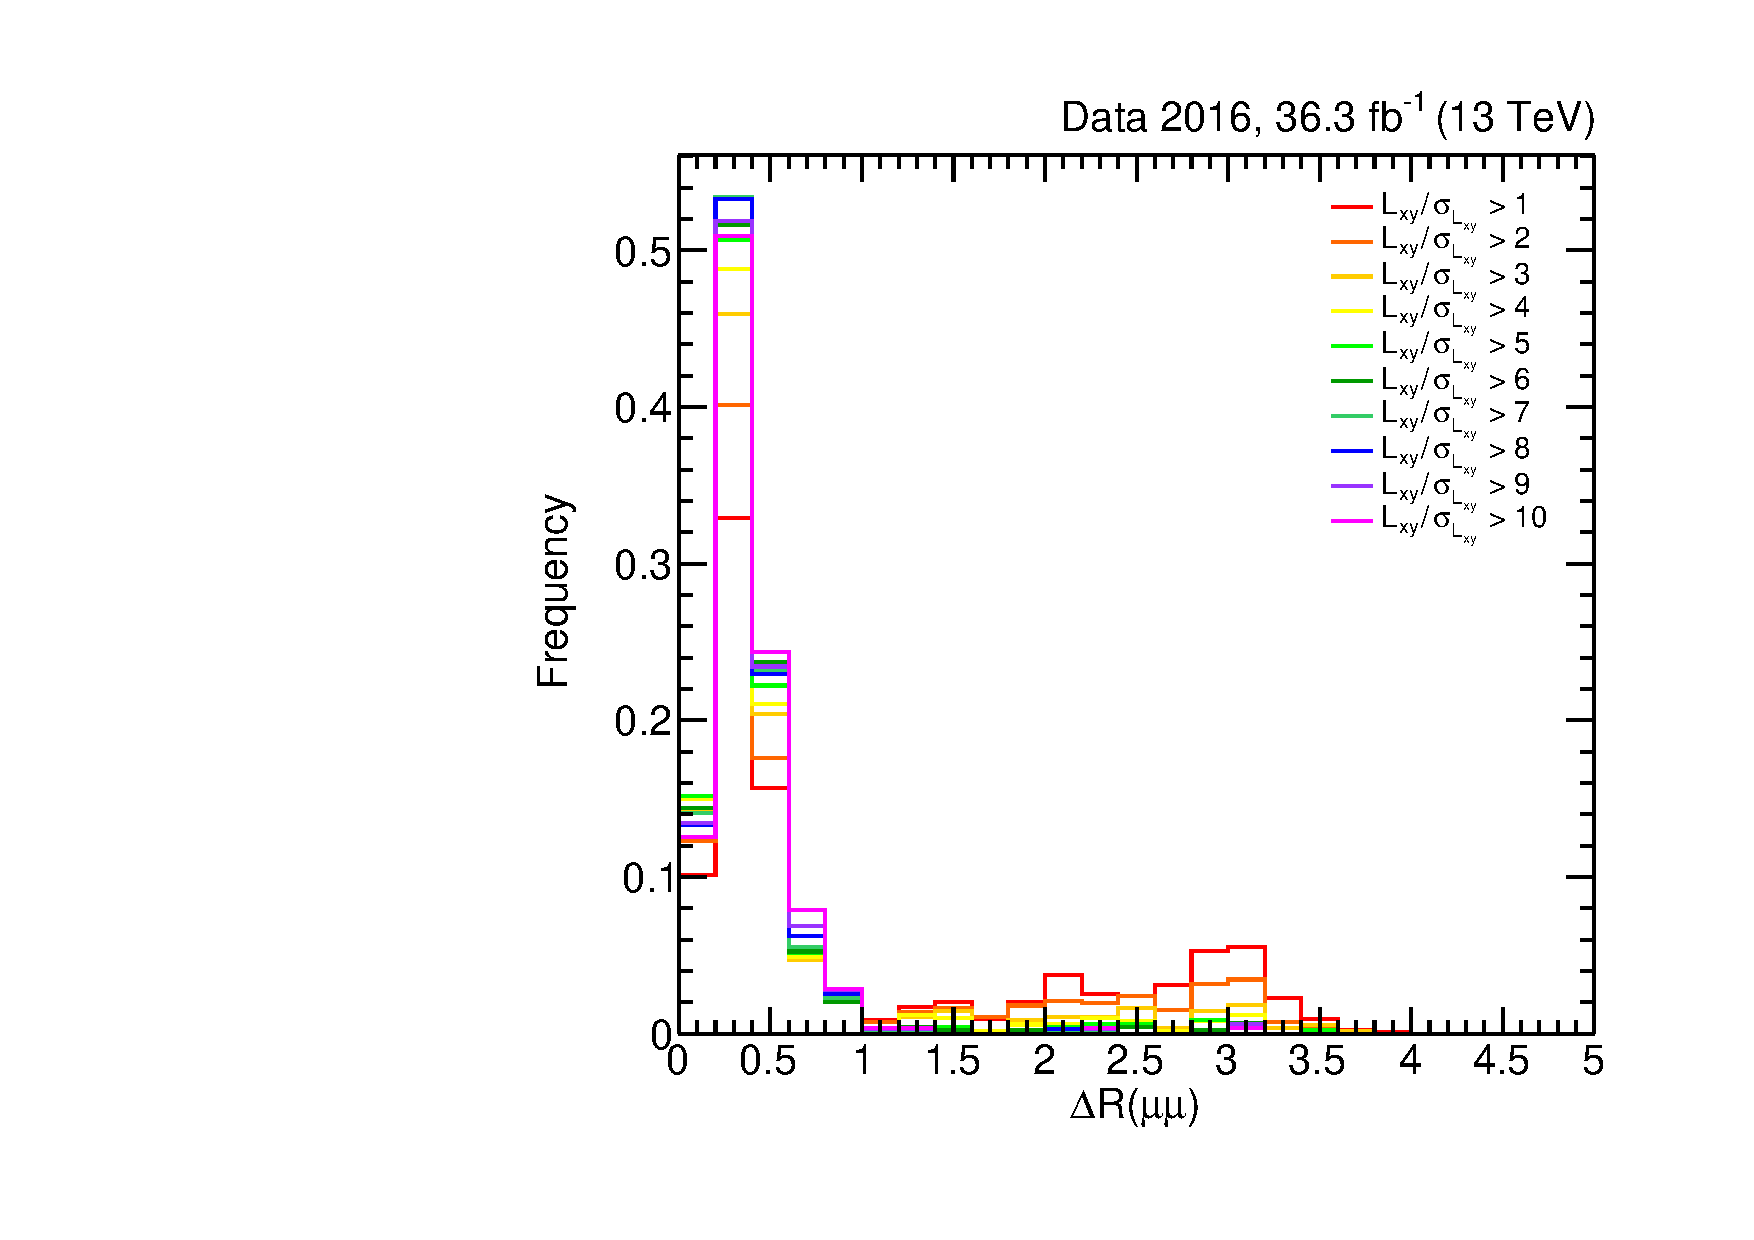
\includegraphics[width=\DSquareWidth]{figures/displaced/BGEST_EffectOfLxySigCut_DeltaR_Data_QCD-Like.pdf}
  \caption[Histograms of \mMuMu and $\deltaR(\Pgm\Pgm)$ for QCD-like events in data for sequentially increasing cut values of \LxySig.]{Histograms of \figpos{left} \mMuMu and \figpos{right} $\deltaR(\Pgm\Pgm)$ as in \Fig~\ref{fig:dd:SeqLxySig_DY_MassDeltaR}, but for QCD-like events in data, using the control regions \CR{QCD}{>x}{0} for variable, sequentially increasing cut values $x$ of DSA \LxySig.}
  \label{fig:dd:SeqLxySig_QCD_MassDeltaR}
\end{figure}

Such QCD-like events hence would not appear in control regions with low \LxySig or high \DeltaPhi, and estimation of this background cannot be performed with a transfer factor applied to events in \CR{\Full}{>6}{\pi}.

Instead, pairs of regions with same-sign dimuons and opposite-sign dimuons are considered.
\Tab~\ref{tab:dd:QCDcontrolregions} gives the number of events in data for several control regions.
The relevant control regions are then \CR[OS]{QCD}{>6}{0} and \CR[SS]{QCD}{>6}{0}, and the transfer factor obtained thus can be applied to \CR[SS]{\Full}{>6}{0} to obtain a QCD background estimate for \CR[OS]{\Full}{>6}{0}.
This transfer factor has a value of
\begin{equation}
  \TF_\text{QCD} = \frac{N\left[\CR[OS]{QCD}{>6}{0}\right]}{N\left[\CR[SS]{QCD}{>6}{0}\right]} = 2.81
  \label{eq:dd:QCDtransferfactor}
\end{equation}

There are 4 same-sign events in \CR[SS]{QCD}{>6}{0} in the full 2016 dataset, giving an estimate of QCD background in the SR of 11.2 events (without the mass window cuts described in \Sec~\ref{sec:dd:cutopt_mass}).
As with the Drell-Yan transfer factor, there is a large systematic uncertainty on the QCD transfer factor (among other factors, it is sensitive to the window used for the PAT \LxySig); this uncertainty will be described and evaluated in \Sec~\ref{sec:dd:bgunc}.

\begin{table}
  \centering
  \begin{tabular}{lcccl}
    \hline
    Name  & Events \\
    \hline
    SR                    & ?   \\
    \CR[SS]{\Full}{>6}{0} & 4   \\
    \CR[OS]{\Full}{<6}{0} & 60  \\
    \CR[SS]{\Full}{<6}{0} & 4   \\
    \CR[OS]{QCD}  {>6}{0} & 323 \\
    \CR[SS]{QCD}  {>6}{0} & 115 \\
    \CR[OS]{QCD}  {<6}{0} & 314 \\
    \CR[SS]{QCD}  {<6}{0} & 196 \\
    \hline
  \end{tabular}
  \caption[Event counts for control regions for estimating QCD background.]{Event counts for control regions for estimating QCD background. A ratio of events in \CR[SS]{QCD}{>6}{0} with same-sign muons to the corresponding control region with opposite-sign muons \CR[OS]{QCD}{>6}{0} gives a transfer factor; multiplying the number of events in \CR[SS]{\Full}{>6}{0} by this transfer factor gives an estimate of the QCD background in SR.}
  \label{tab:dd:QCDcontrolregions}
\end{table}

Other ratios in \Tab~\ref{tab:dd:controlregions} do not give an appropriate transfer factor but rather serve to illuminate features of the QCD background.
The ratio of \CR[OS]{QCD}{<6}{0} to \CR[SS]{QCD}{<6}{0} is 1.6, much closer to 1; this clarifies that there is proportionally more opposite-sign QCD background for large values of \LxySig, and so a large \LxySig region needed to be used to quantify it.
The ratio of \CR[SS]{\Full}{<6}{0} to \CR[OS]{\Full}{<6}{0} is quite small, showing that the same-sign background is not an important contributor to the regions with small \LxySig, and so the same-sign events in this region could not have been used to extrapolate an estimate in the signal region.

\section{Cut Optimization}
This section describes a few procedures applied to fine-tune the event and object selection to optimize the analysis for the statistical significance of a potential signal discovery.

\subsection[Optimizing with \ZBi as a Figure of Merit]{Optimizing with \texorpdfstring{$\bm{Z_{\mathbf{Bi}}}$}{ZBi} as a Figure of Merit}
\label{sec:dd:cutopt_ZBi}
As a set of analysis selections varies, the numbers of signal and background events also vary, and so fine-tuning the values of cuts is an exercise in balancing signal efficiency \vs background rejection.
The metric for determining an optimal cut value, as a function of the number of signal and background events, is a figure of merit that is monotonic with the expected statistical significance of a discovery.
The figure of merit used in this analysis is \ZBi \cite{Cousins:ZBi2008}, an estimate of the statistical significance of an excess number of events in a signal region when the number of background events is estimated from a control region.
The subscript is an abbreviation for \textbf{Bi}nomial, because under the background-only hypothesis, the splitting of events between the signal and control region follows a binomial distribution with binomial parameter equal to the expected fraction of background in the signal region out of the background in both regions.
In the notation introduced in \Sec~\ref{sec:dd:bgest}, with \TF the transfer factor, this binomial parameter is $1/(1+\TF)$.

A procedure based on \ZBi as a figure of merit was performed on several key discriminating variables.
The following description of the procedure will be phrased in terms of optimizing the \LxySig cut.
A background distribution of \LxySig is defined as a histogram of data events in the (approximately) signal-free region $\DeltaPhi > \pi/2$, and a corresponding signal distribution of \LxySig is defined as a histogram of signal events in the signal region \mbox{$\DeltaPhi < \pi/2$}, with both distributions consisting of events passing all selections except for the \LxySig cut.
The signal histogram is scaled to 2016 integrated luminosity assuming an arbitrary production cross section of $1\times 10^{-2}\unit{pb}$.
For \LxySig, the number of events in either histogram passing a given cut is an integral from the cut value to infinity; for some other variables (such as track \normchisq), the number of events passing a given cut is an integral from zero to the cut value.
In the following discussion, the ``integral'' of a histogram is assumed to be performed over the appropriate interval.

In the notation found in Reference~\cite{Cousins:ZBi2008}, the integral of the simulated signal histogram corresponds to ${\mu}_s$, the true Poisson mean number of signal events in the signal region;
and the integral of the background histogram corresponds to a number of observed events in the signal-free region $n_\text{off}$, from which one derives the estimate $\hat{\mu}_b = n_\text{off}/\TF$ of the true Poisson mean number of background events in the signal region.
To obtain the median \ZBi, $\mu_s$ is used as the estimate of the true Poisson signal mean $\hat{\mu}_s$.
\ZBi is then calculated for each cut value, a function of three quantities: the number of background events in the control region $n_\text{off}$, the total number of observed events in the signal region $n_\text{on} = \hat{\mu}_s + \hat{\mu}_b$, and the transfer factor is taken to be $\TF = 1$.

\Fig~\ref{fig:dd:CutOptExample} shows an example of the cut optimization procedure, with the background (control region in data) distribution in red, the signal distribution (here for the \twoMu signal sample with \FullSP{1000}{20}{20}) in blue, and the value of \ZBi for each cut value in green.
The tail of the signal distribution is much longer than in the background distribution, which peaks strongly at smaller values of \LxySig, so \ZBi rises steadily until about 5 or 6.
For this signal sample, the cut value of \LxySig corresponding to the largest value of \ZBi is between 6 and 7.

\begin{figure}[htpb]
  \centering
  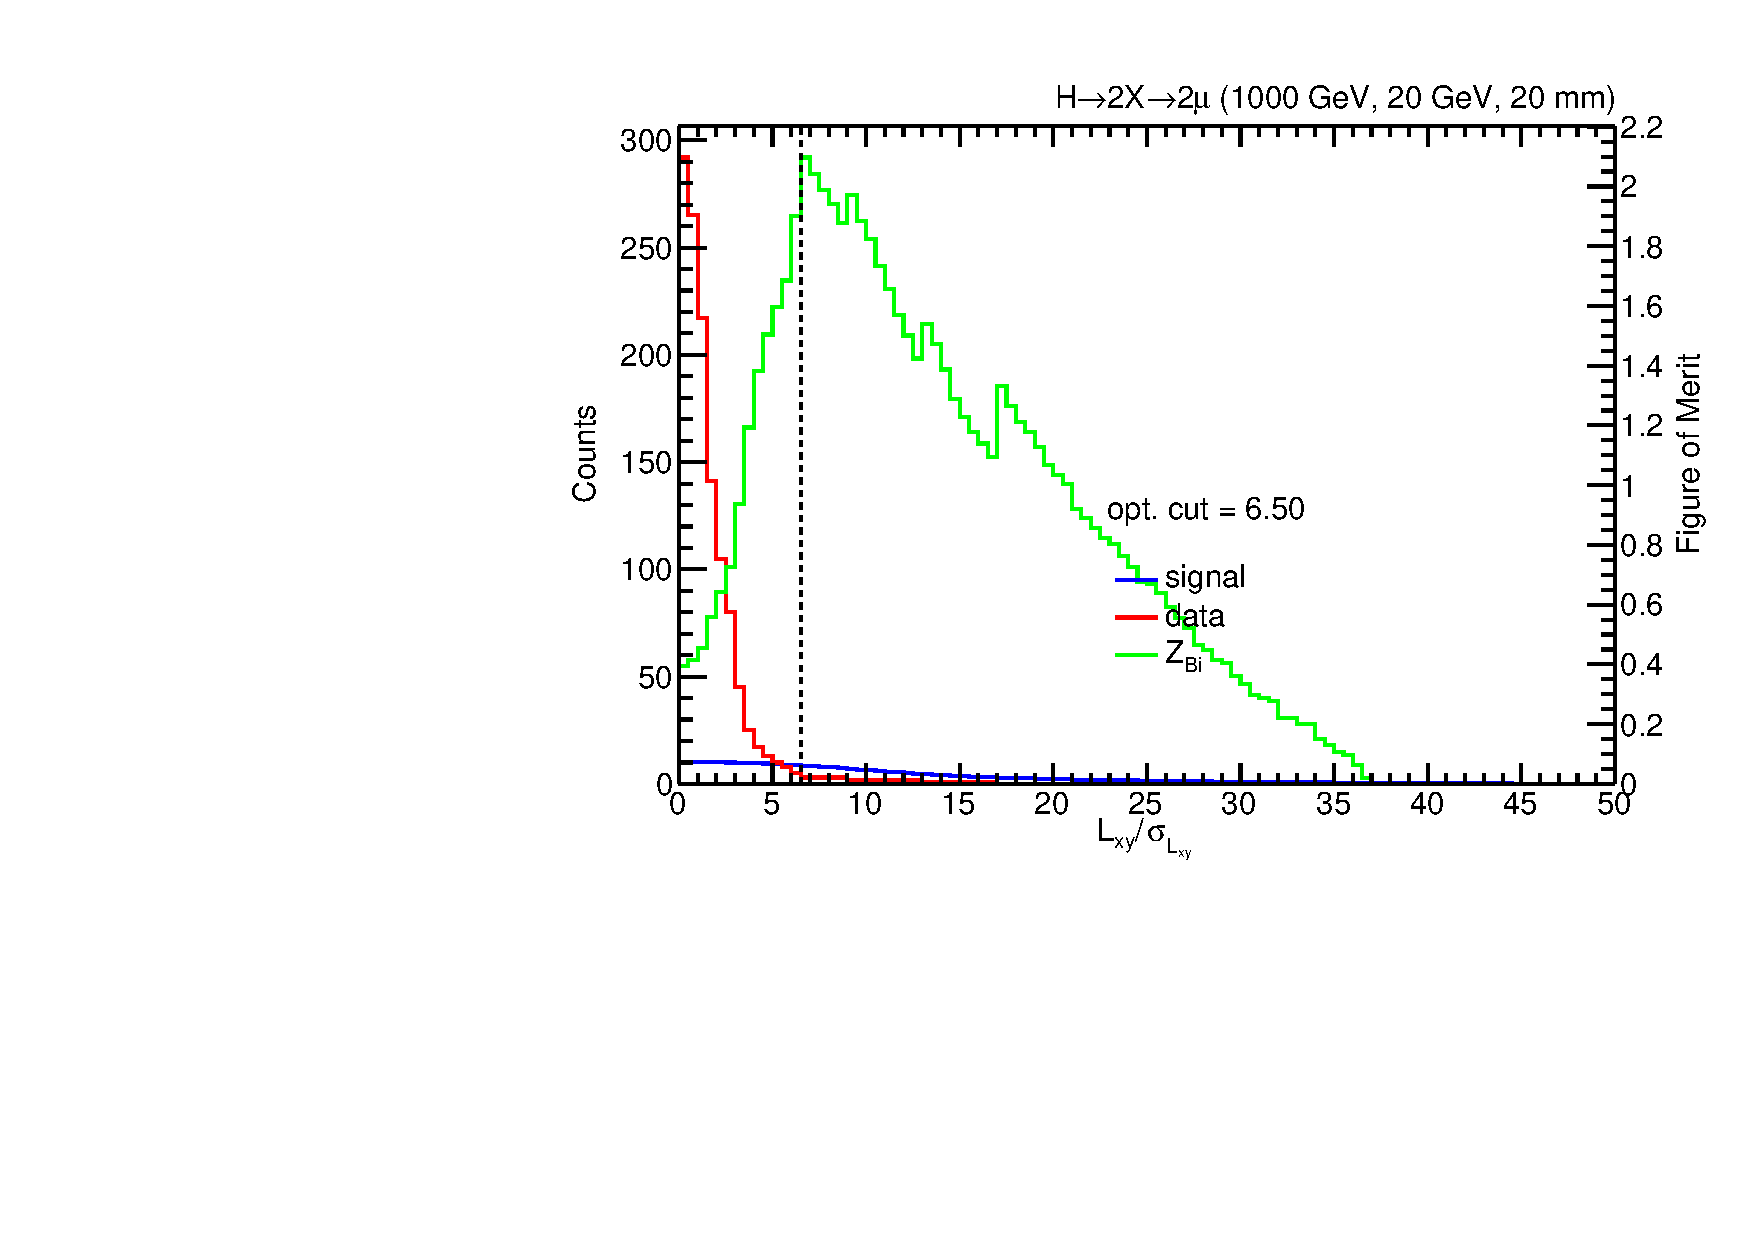
\includegraphics[width=\DFigWidth]{figures/displaced/OPT_LxySig_ZBi_HTo2XTo2Mu2J_1000_20_20.pdf}
  \caption[Example of \ZBi-based cut optimization of \LxySig.]{Example of \ZBi-based cut optimization of \LxySig for the \twoMu signal sample with \FullSP{1000}{20}{20}. The background distribution is in red and corresponds to a selection of events in a control region of data; the signal distribution is in blue; and the value of \ZBi at each cut value is in green. Here, the cut value of \LxySig corresponding to the largest value of \ZBi is between 6 and 7, marked on the plot as 6.5. As a consequence of the background distribution having a strong peak at small values of \LxySig and the tail in the signal distribution being much longer, the \ZBi curve rises steadily for tighter cuts on \LxySig, peaks, and then falls.}
  \label{fig:dd:CutOptExample}
\end{figure}

This procedure was performed on all signal samples, with a systematic grid of cut values in several variables.
The main results of this \ZBi-based cut optimization are:
\begin{itemize}
  \item \ZBi rises steadily as cuts on \LxySig and track \normchisq are tightened, informing the choices of cut values of 6 and 2.5, respectively. Although for some sets of selections, \ZBi continues to increase for tighter cuts, the shape flattens out considerably after these thresholds, so the increases in \ZBi are minimal, and the shape becomes highly sensitive to the specific background events and the specific numbers of events used to tune the cuts. The choices of cut values take these effects into account.
  \item \ZBi does not increase appreciably for any requirement on the muon track impact parameter significance ($d_0/\sigma_{d_{0}}$) once a requirement on \LxySig requirement is in place, so the analysis selection does not impose any cuts on $d_0/\sigma_{d_{0}}$. This was a requirement that was used in previous versions of this analysis performed with Run 1 data \cite{EXO-12-037,CMS-PAS-EXO-14-012}. Similarly, no appreciable increase in \ZBi was observed for tighter cuts on vertex \chisq than 20 once other cuts are in place.
\end{itemize}

\subsection{Dimuon Mass Window Selection}
\label{sec:dd:cutopt_mass}
When computing upper limits on long-lived particle production cross sections, it is undesirable to include in the observation dimuon events with invariant masses appreciably different from the invariant mass postulated by the signal model under consideration.
To implement this requirement, the reconstructed dimuon invariant mass histograms (for each value of generated long-lived particle mass \mX, for events passing the full selection in \twoMu signal) are fit to Gaussian distributions, yielding a mean and standard deviation, $\mu_{\mX}$ and $\sigma_{\mX}$.
\Fig~\ref{fig:dd:massdistributions} shows the distributions of reconstructed dimuon mass for \twoMu signal samples, combining all sets of signal parameters for each value of \mX, for events passing all selections except for the mass cut, along with a fitted Gaussian for each distribution.
The dimuon invariant mass is required to lie within a mass window given by $\mu_{\mX} \pm 3\sigma_{\mX}$, with the lower limit at least 10\GeV and no upper limit for the largest generated mass.
This selection is more than 99\% efficient in most \twoMu signal samples (97\% in the worst case).
\Tab~\ref{tab:dd:masswindow} enumerates the invariant mass window selection (applied to reconstructed dimuons) used for each generated value of \mX.

\begin{figure}[htbp]
  \centering
  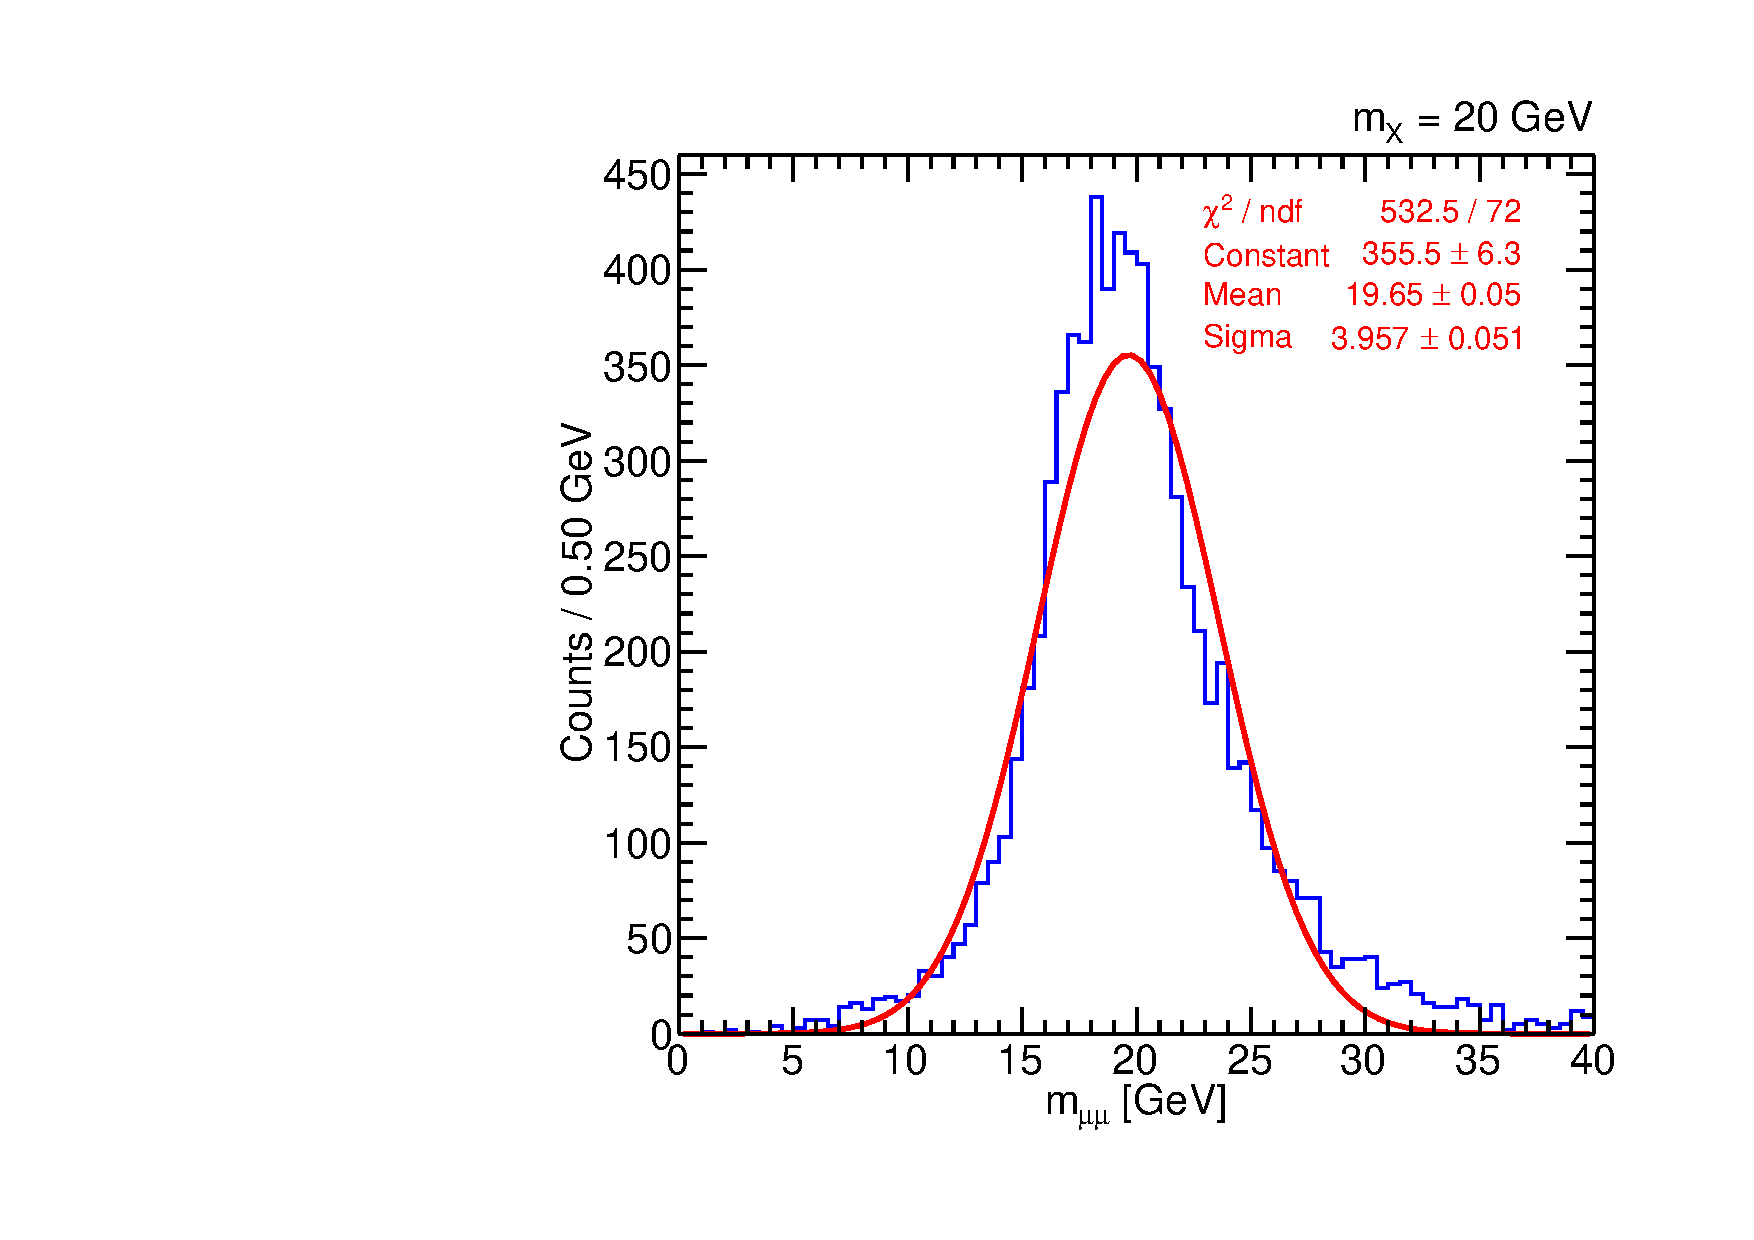
\includegraphics[width=\DSquareWidth]{figures/displaced/MASS_2Mu2J_20.pdf}
  \hspace*{-2em}
  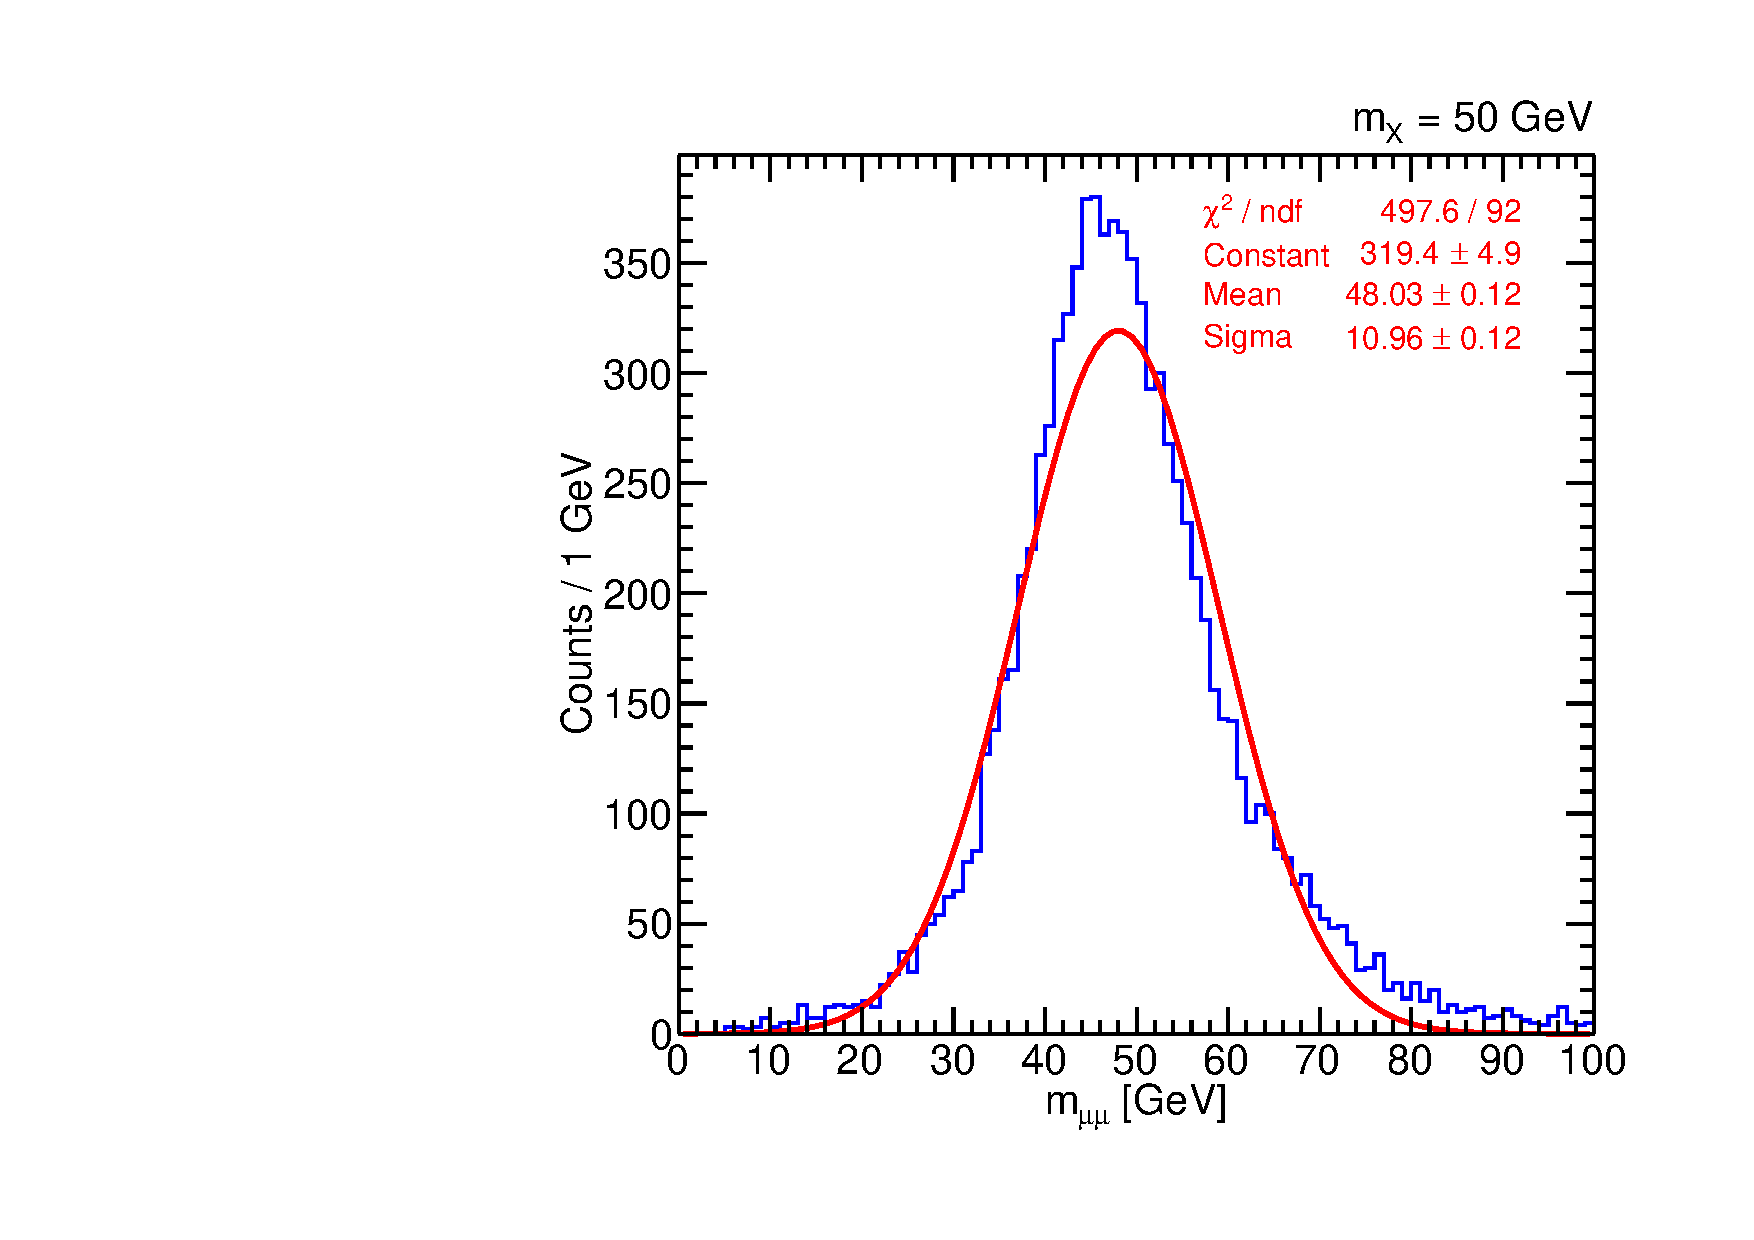
\includegraphics[width=\DSquareWidth]{figures/displaced/MASS_2Mu2J_50.pdf} \\
  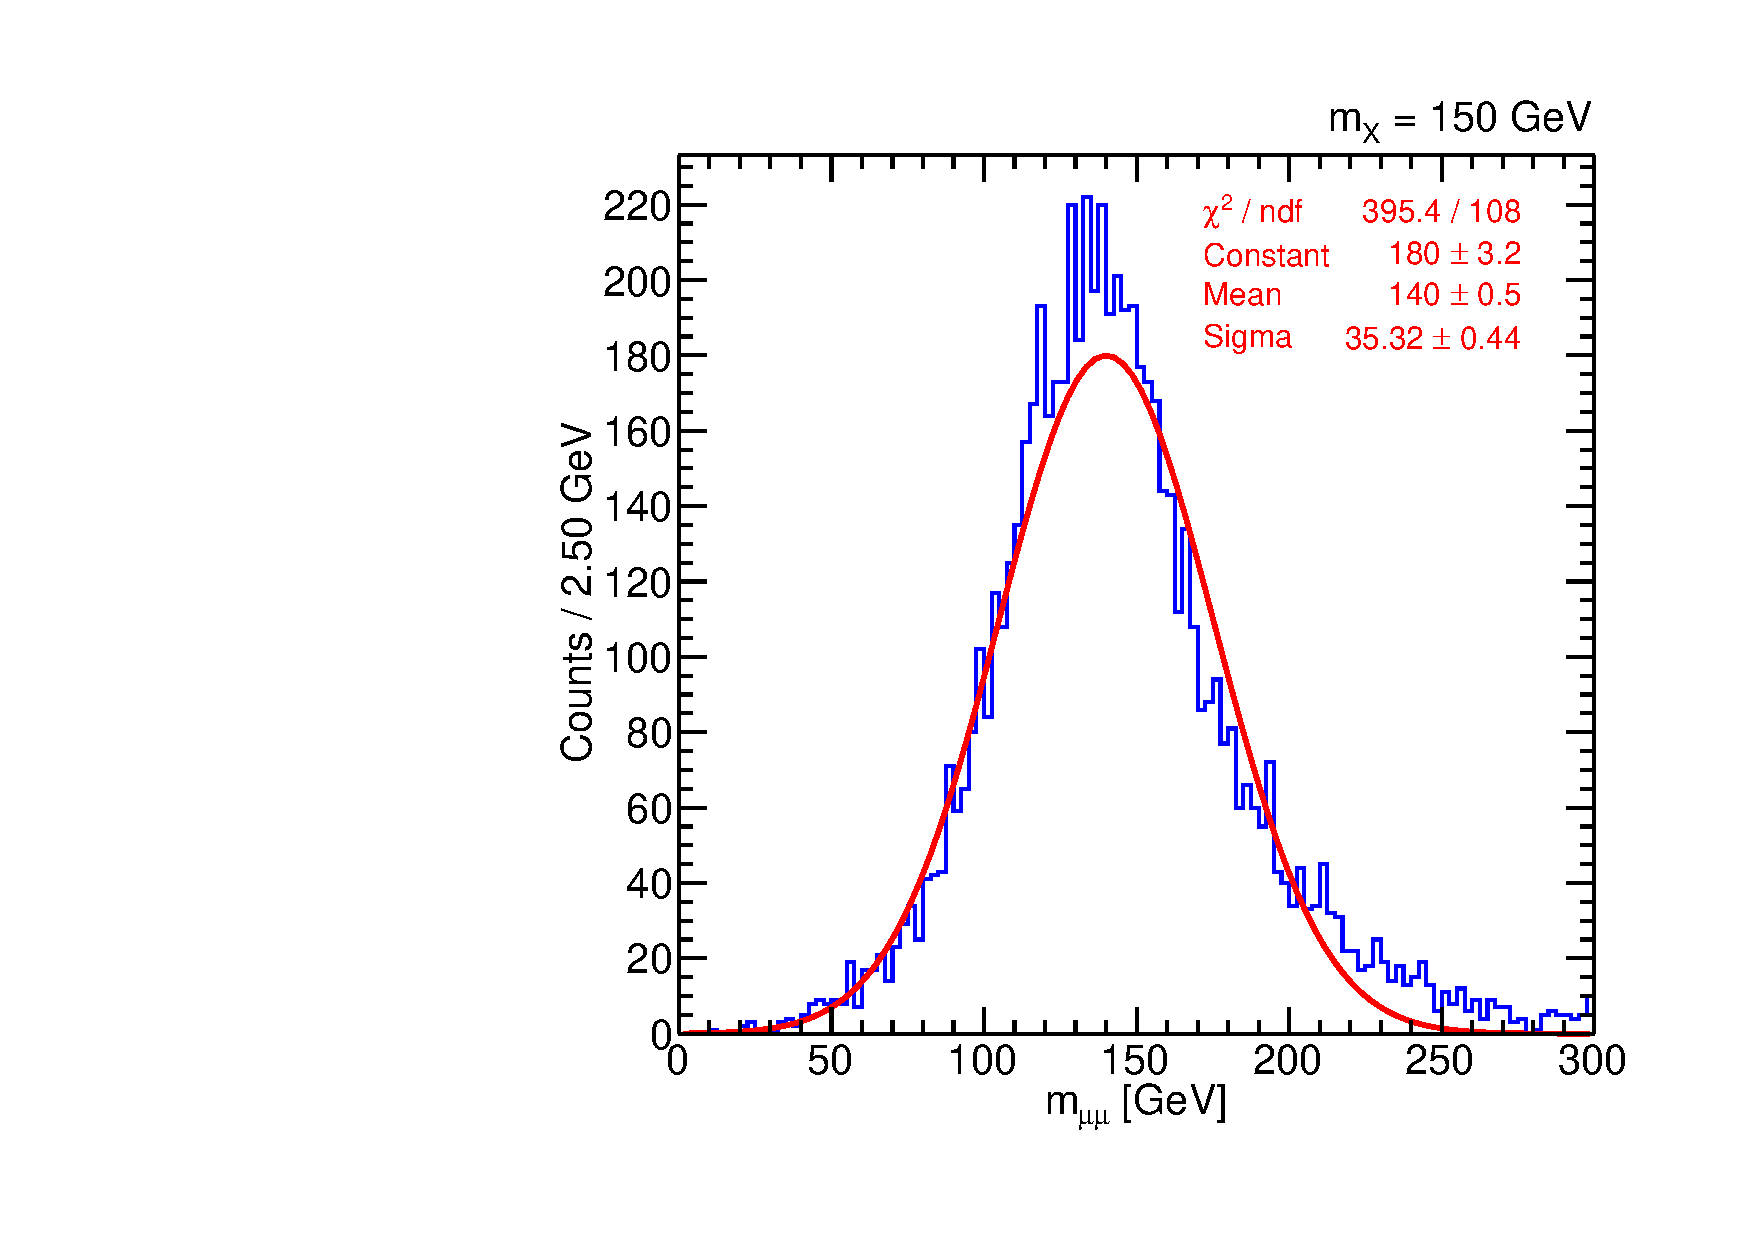
\includegraphics[width=\DSquareWidth]{figures/displaced/MASS_2Mu2J_150.pdf}
  \hspace*{-2em}
  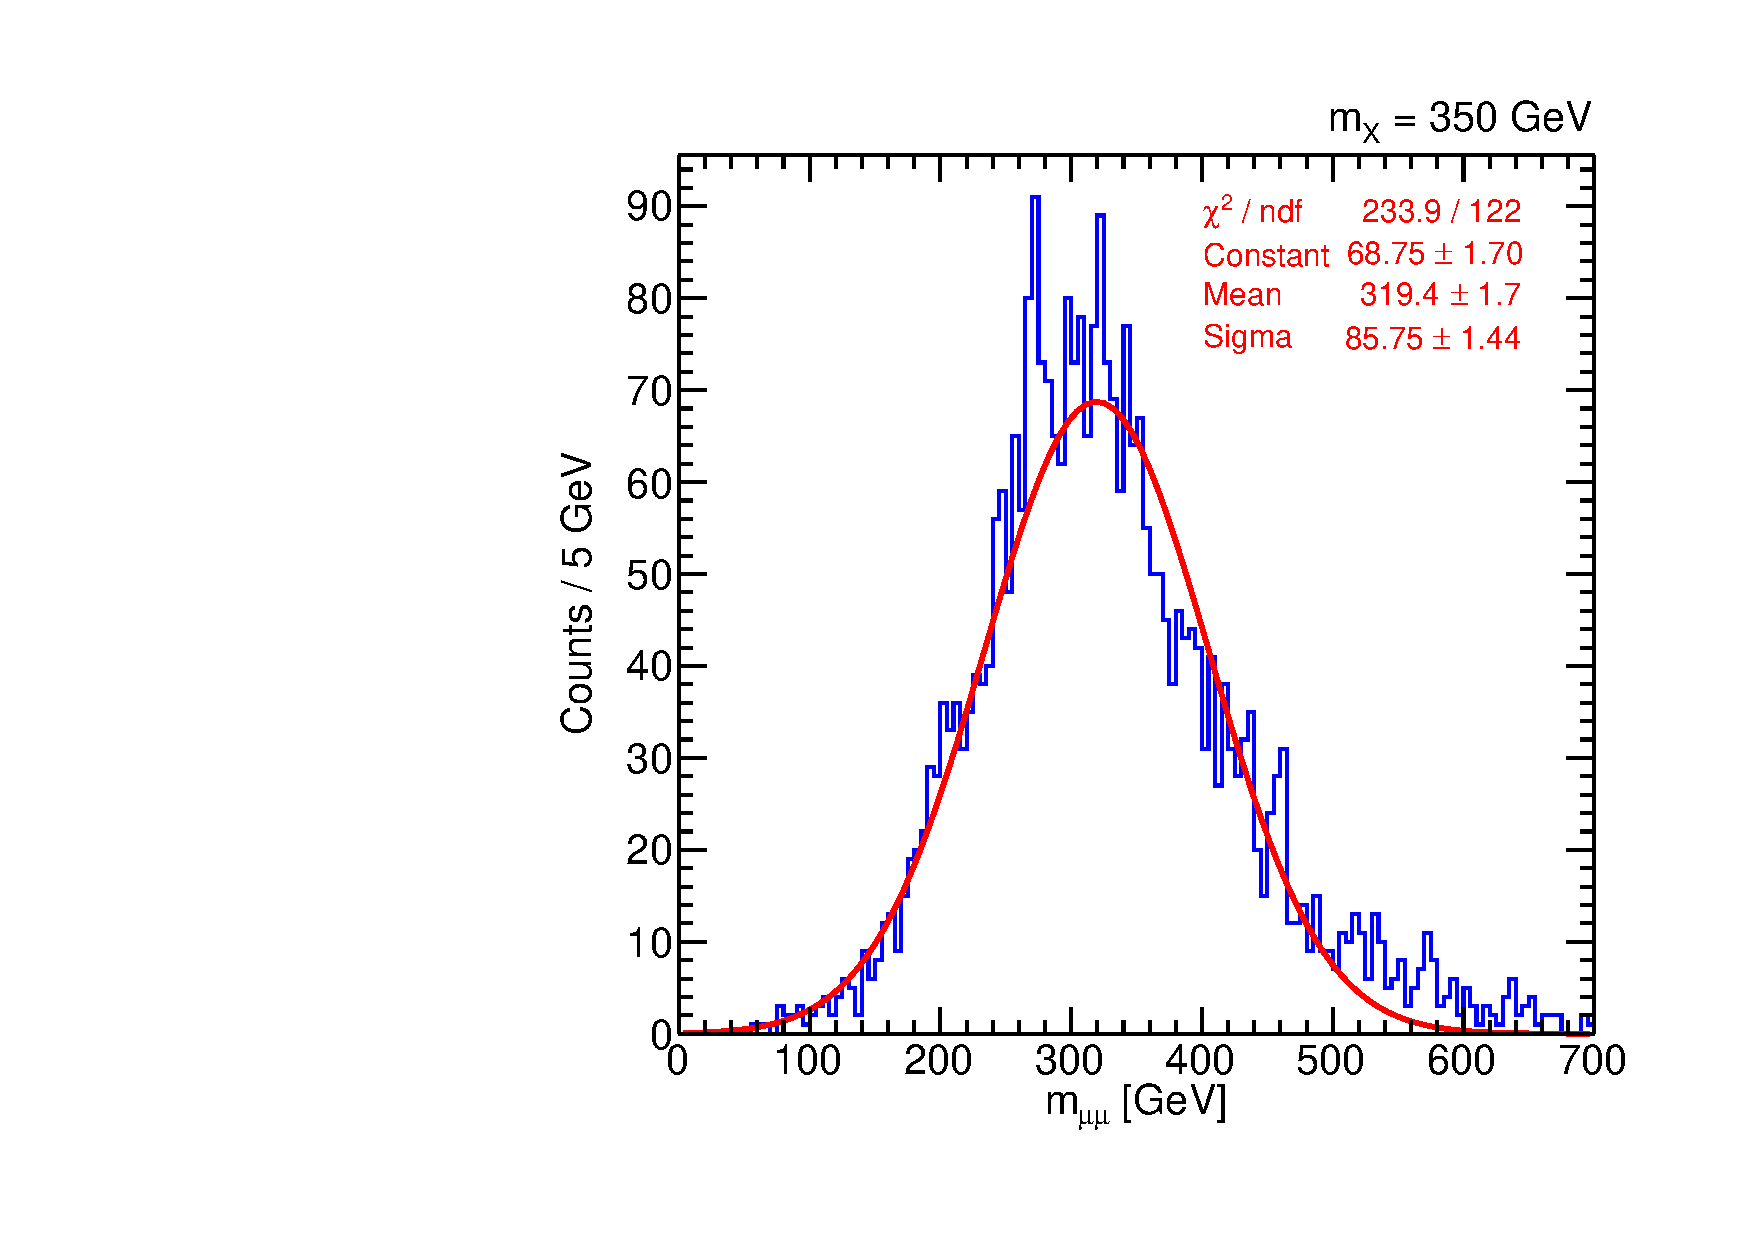
\includegraphics[width=\DSquareWidth]{figures/displaced/MASS_2Mu2J_350.pdf}
  \caption[Reconstructed invariant dimuon mass distributions for \twoMu signal samples, long with fitted Gaussian curves for each distribution.]{Reconstructed invariant dimuon mass distributions for \twoMu signal samples passing all selections except the mass cut, combining all sets of signal parameters for each value of \mX, along with fitted Gaussian curves for each distribution.}
  \label{fig:dd:massdistributions}
\end{figure}

\begin{table}
  \centering
  \begin{tabular}{rrrl}
    \hline
    Generated \mX & \multicolumn{1}{c}{$\mu$} & \multicolumn{1}{c}{$\sigma$} & Dimuon Mass Window           \\
    \hline
     20\GeV       &  20\GeV &   4\GeV & $10\GeV < \mMuMu < 32\GeV$   \\
     50\GeV       &  50\GeV &  10\GeV & $20\GeV < \mMuMu < 80\GeV$   \\
    150\GeV       & 140\GeV &  35\GeV & $35\GeV < \mMuMu < 245\GeV$  \\
    350\GeV       & 320\GeV &  85\GeV & $65\GeV < \mMuMu$            \\
    \hline
  \end{tabular}
  \caption[Dimuon invariant mass window selections for each value of generated long-lived particle mass \mX.]{Dimuon invariant mass window selections for each value of generated long-lived particle mass \mX, along with values for the fitted Gaussian $\mu$ and $\sigma$. The windows are defined as $\mu \pm 3\sigma$ with the lower limit at least 10\GeV and no upper limit for the largest generated mass.}
  \label{tab:dd:masswindow}
\end{table}

\subsection{N--1 Plots}
This section presents selected ``N$-$1'' plots, so named because they are histograms of events passing the full selection except for one cut: the variable plotted.
Such plots depict the events that passed all other cuts and would be removed by applying the cut in question, and so convey the effect of individual cuts in the analysis.
These plots also provide a structured way of comparing the distributions and the fraction of events passing each cut in signal and background.
The analysis selections should be highly efficient in signal and highly inefficient in background.

\Figs~\ref{fig:dd:NM1_pT}--\ref{fig:dd:NM1_LxySig} are the N$-$1 plots for selected variables, for events in all \twoMu signal samples combined and for events in the control region \CR{\Full}{>6}{\pi} of data.
The cut values are labeled on the plots, as is the efficiency of the selection.
The cosmic rejection cuts on $\cos{\alpha}$ and number of parallel pairs are highly correlated, and so the corresponding plots, \Fig~\ref{fig:dd:NM1_cosAlpha} and \Fig~\ref{fig:dd:NM1_Npp}, omit both cuts from both sets of plots; for this reason they are actually ``N$-$2'' plots.

\begin{figure}[p]
  \centering
  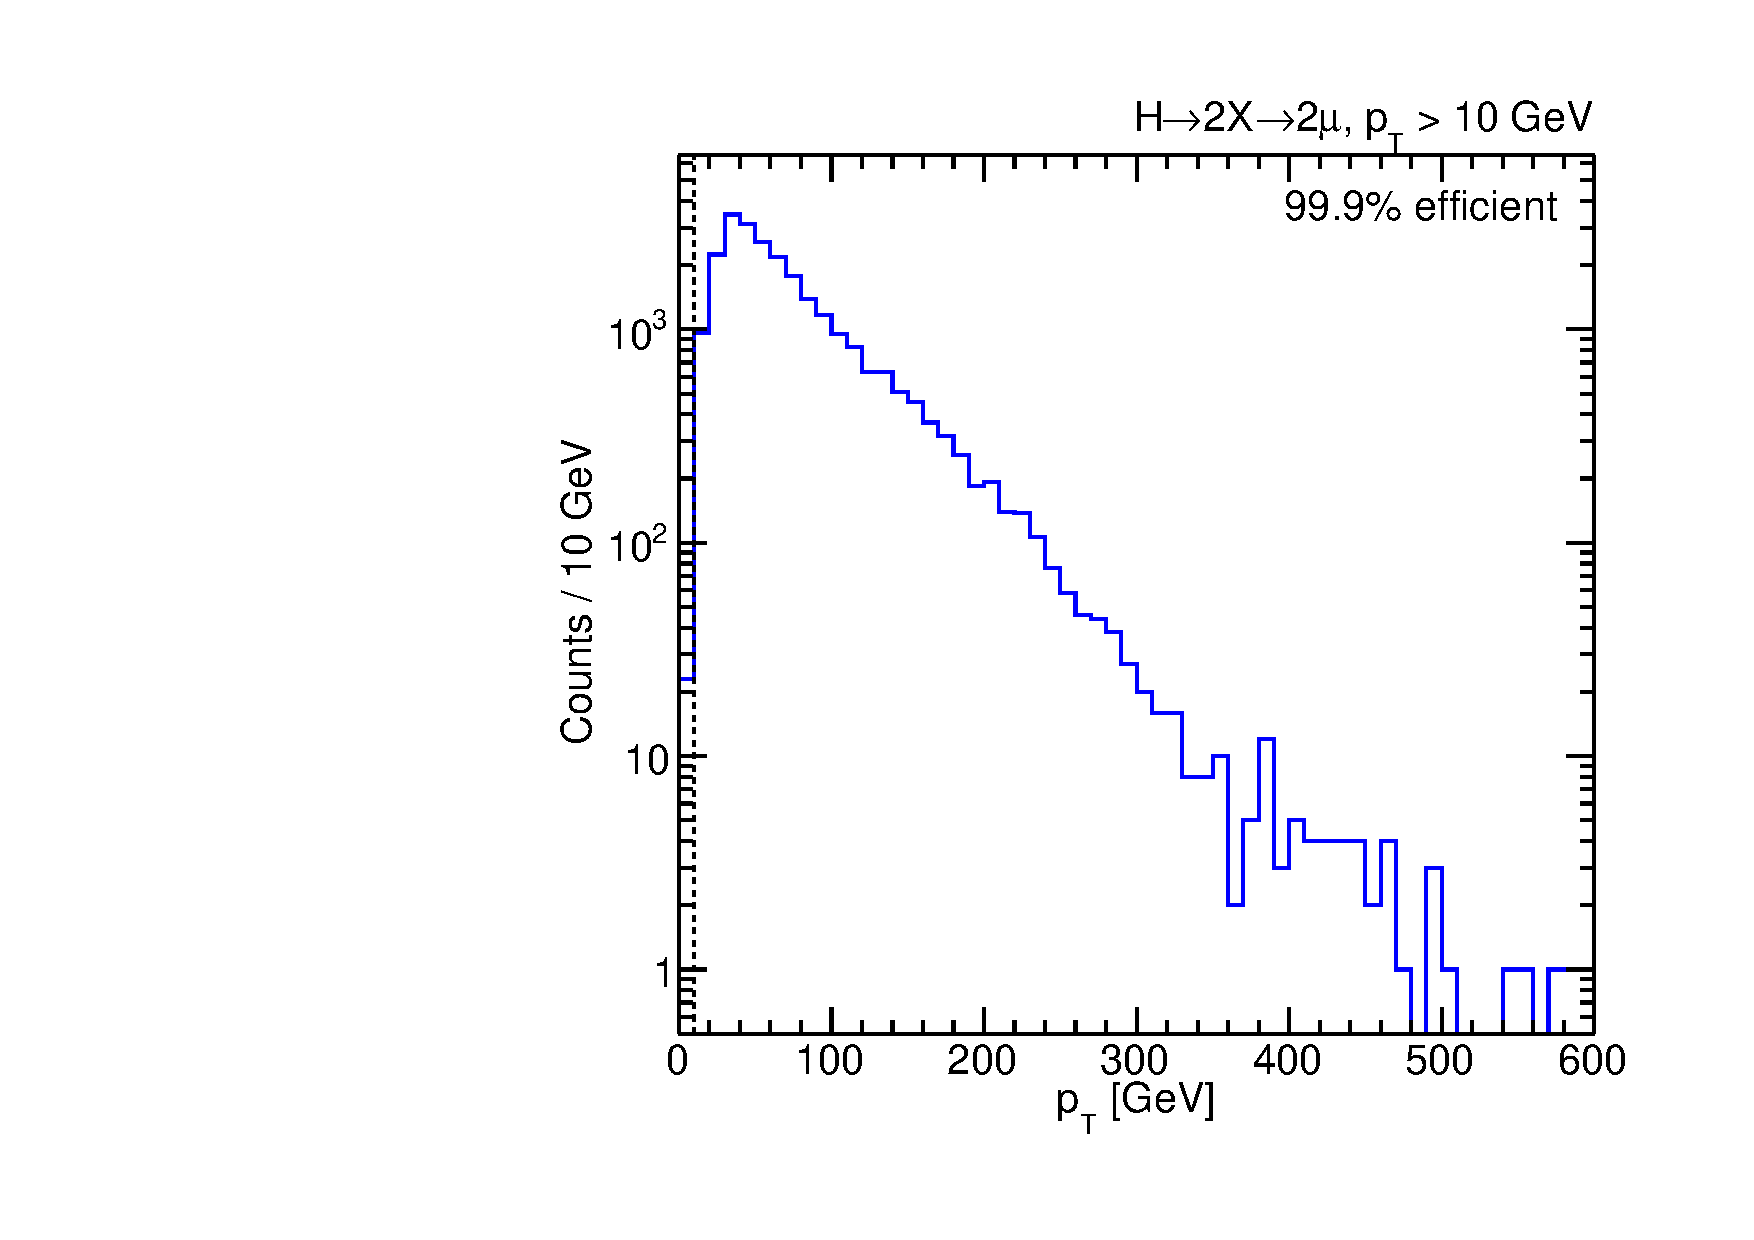
\includegraphics[width=\DSquareWidth]{figures/displaced/NM1_2Mu2J_pT.pdf}
  \hspace*{-2em}
  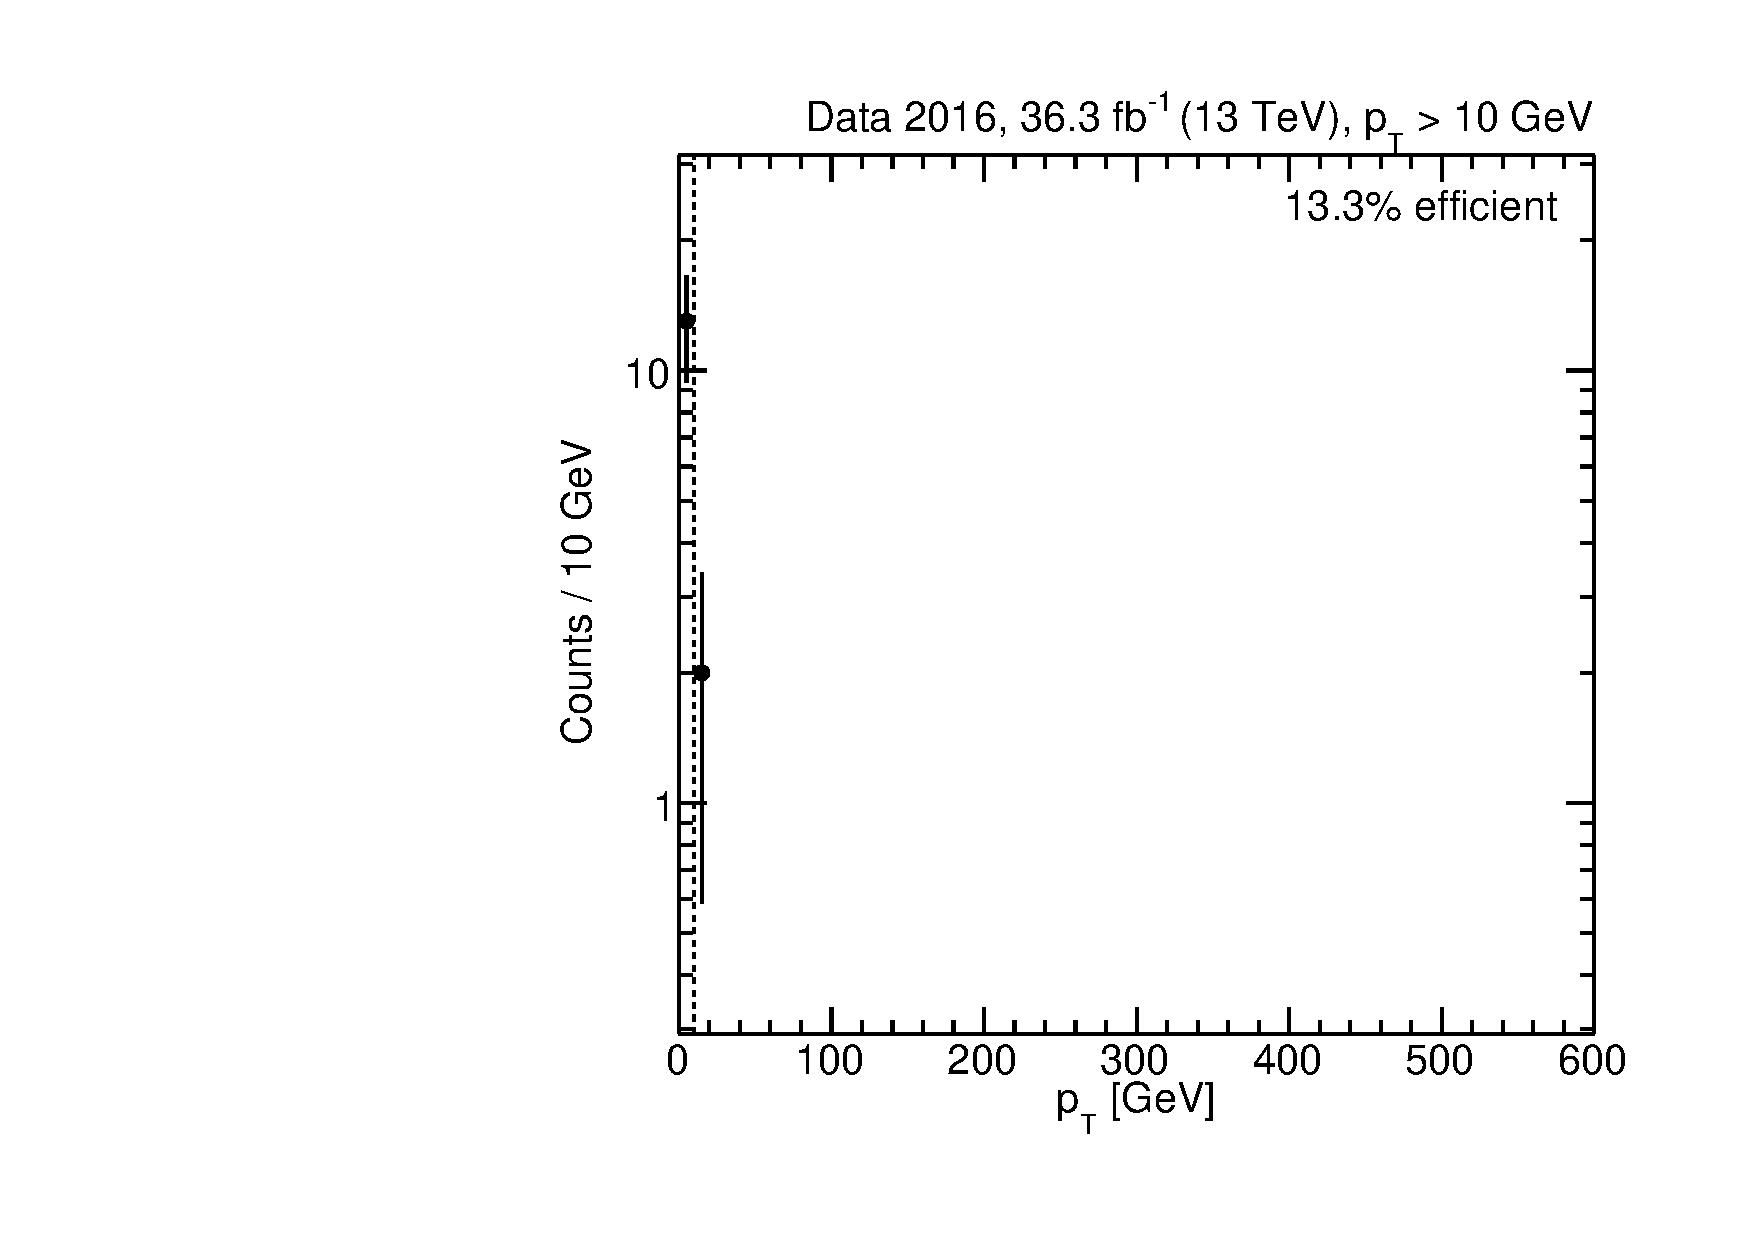
\includegraphics[width=\DSquareWidth]{figures/displaced/NM1_Data_pT.pdf}
  \caption[Histograms of events passing the full selection except for the muon \pT cut in \twoMu signal and data.]{Histograms of events passing the full selection except for the muon \pT cut, in \figpos{left} \twoMu signal and \figpos{right} data in the control region, along with the labeled cut value (and corresponding dashed line) and the selection efficiency.}
  \label{fig:dd:NM1_pT}
\end{figure}

\begin{figure}[p]
  \centering
  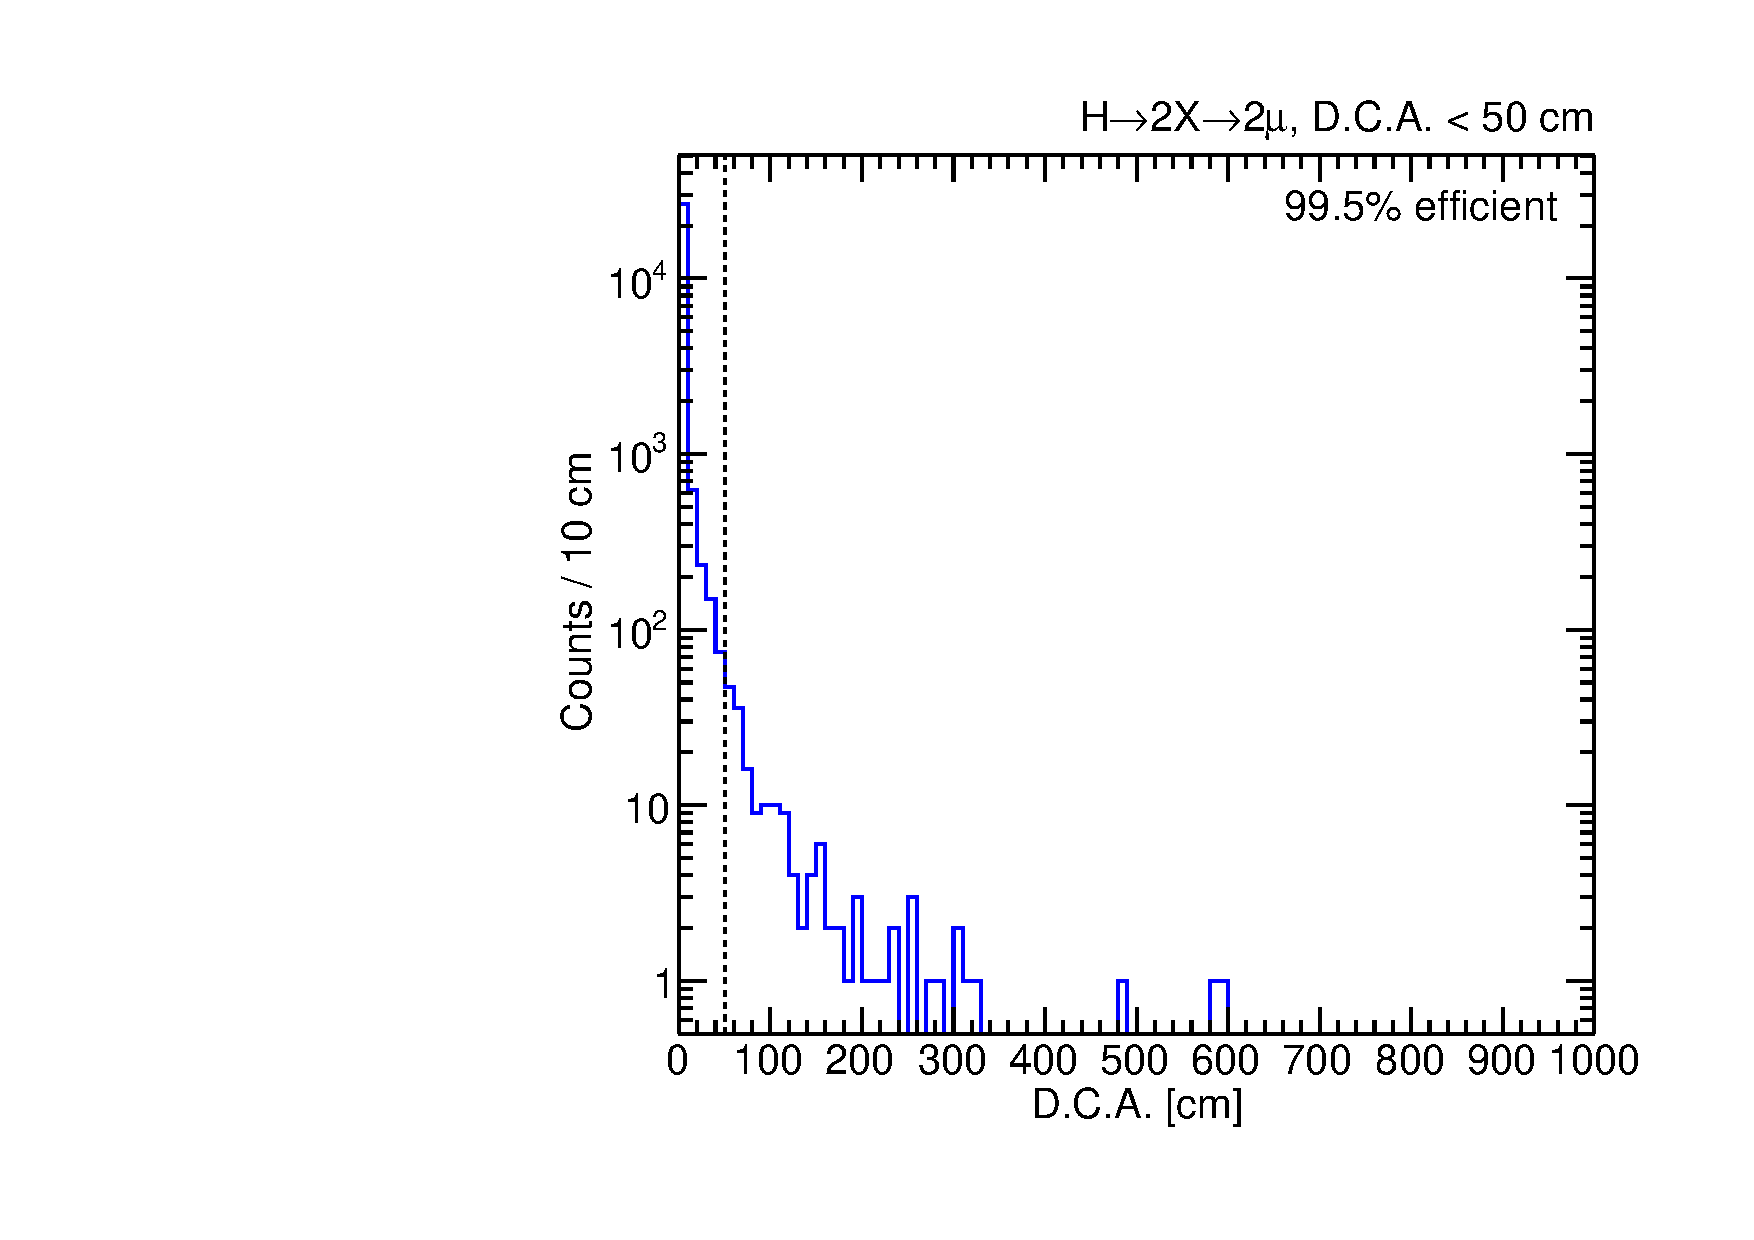
\includegraphics[width=\DSquareWidth]{figures/displaced/NM1_2Mu2J_DCA.pdf}
  \hspace*{-2em}
  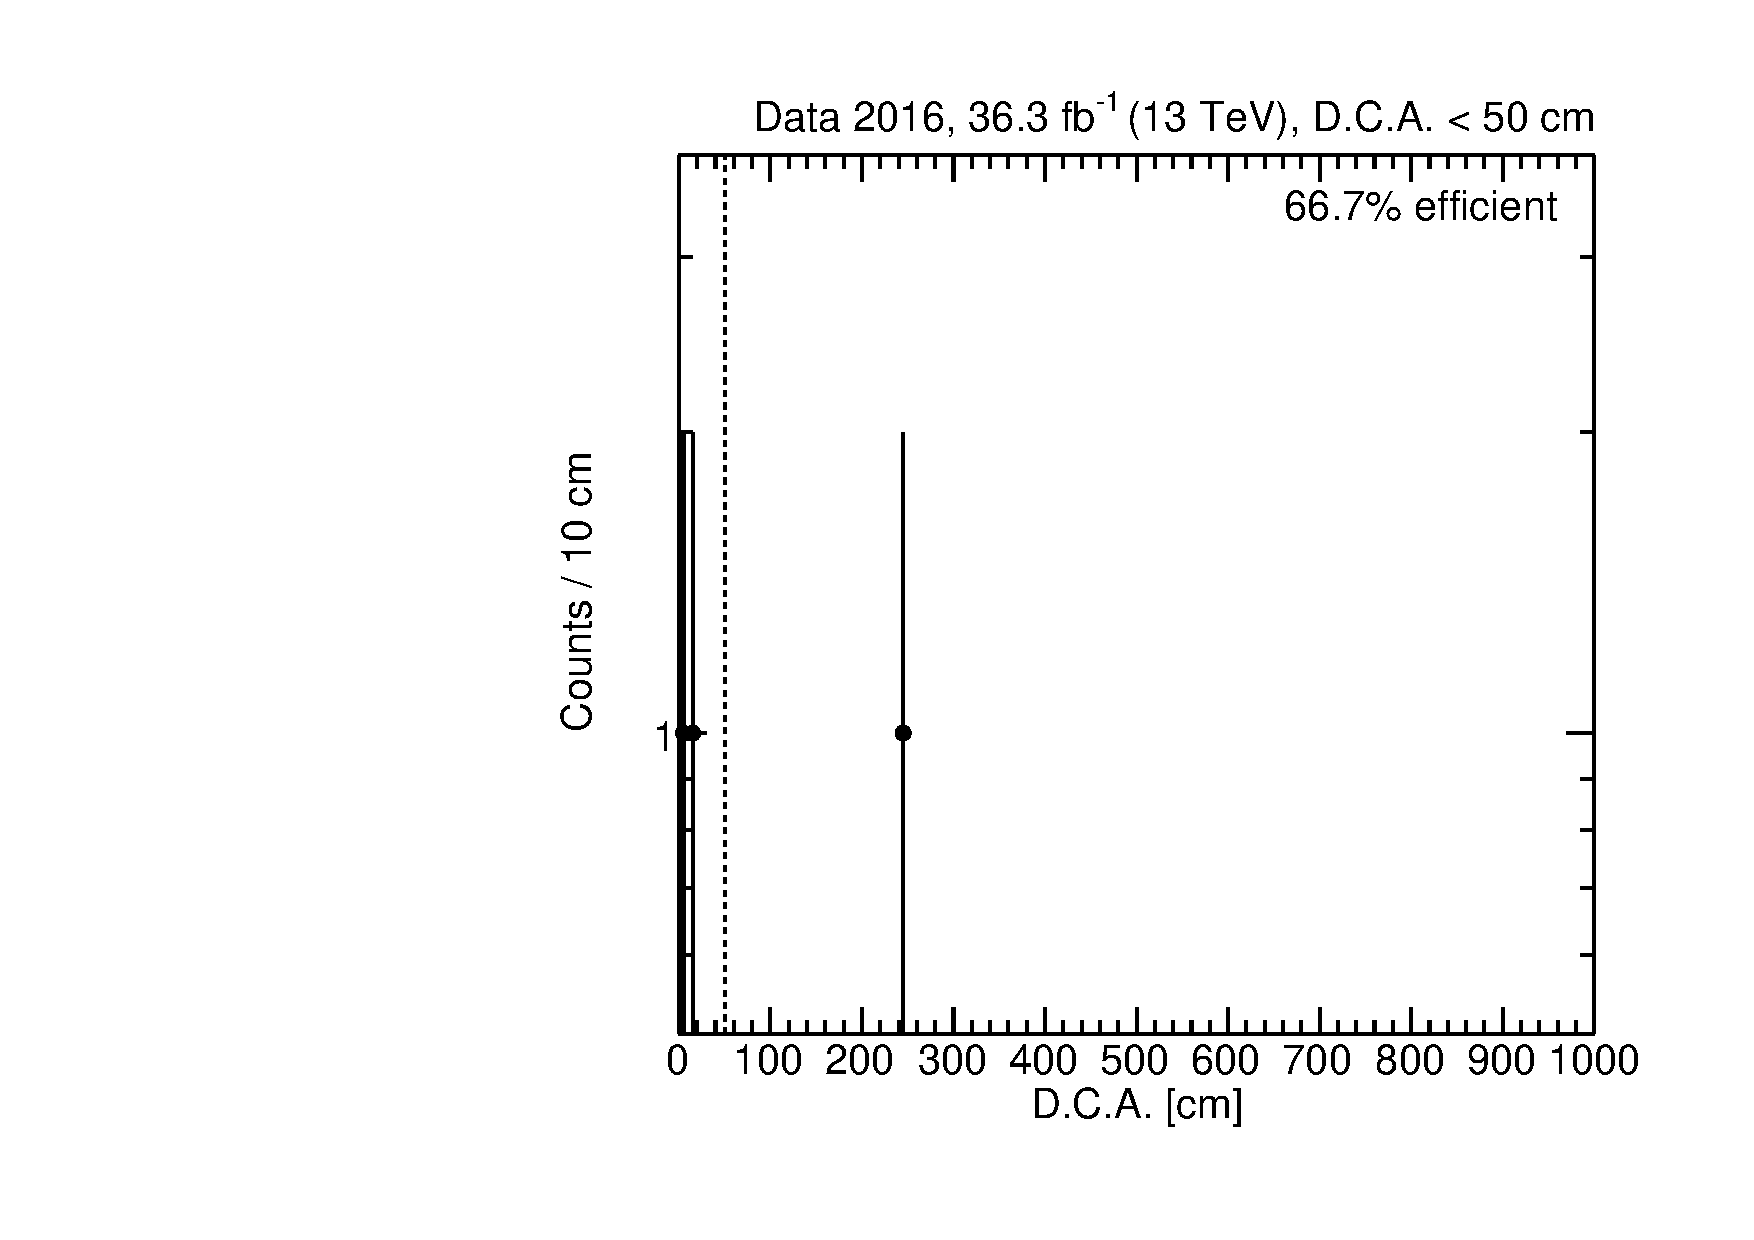
\includegraphics[width=\DSquareWidth]{figures/displaced/NM1_Data_DCA.pdf}
  \caption[Histograms of events passing the full selection except for the distance of closest approach cut in \twoMu signal and data.]{Histograms of events passing the full selection except for the distance of closest approach cut, in \figpos{left} \twoMu signal and \figpos{right} data in the control region, along with the labeled cut value (and corresponding dashed line) and the selection efficiency.}
  \label{fig:dd:NM1_DCA}
\end{figure}

\begin{figure}[p]
  \centering
  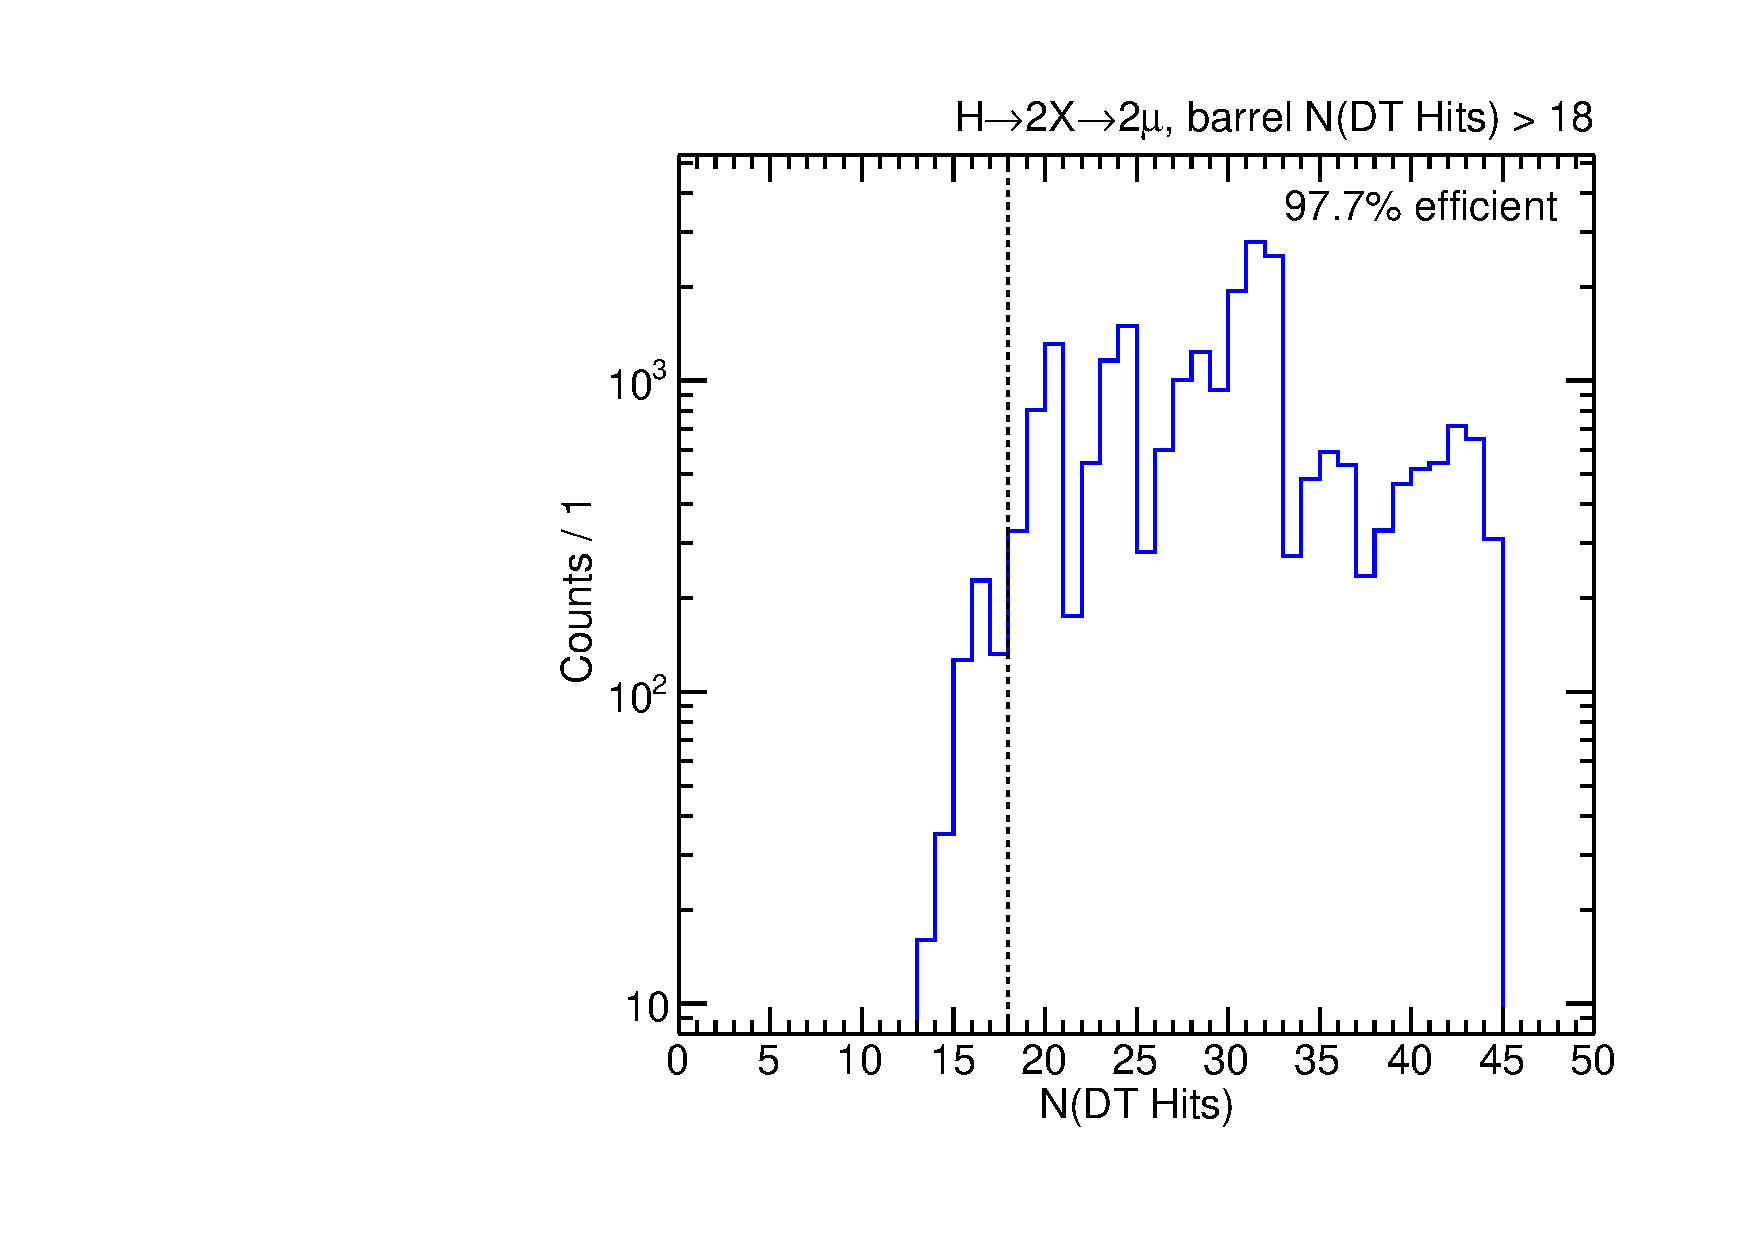
\includegraphics[width=\DSquareWidth]{figures/displaced/NM1_2Mu2J_nDTHits.pdf}
  \hspace*{-2em}
  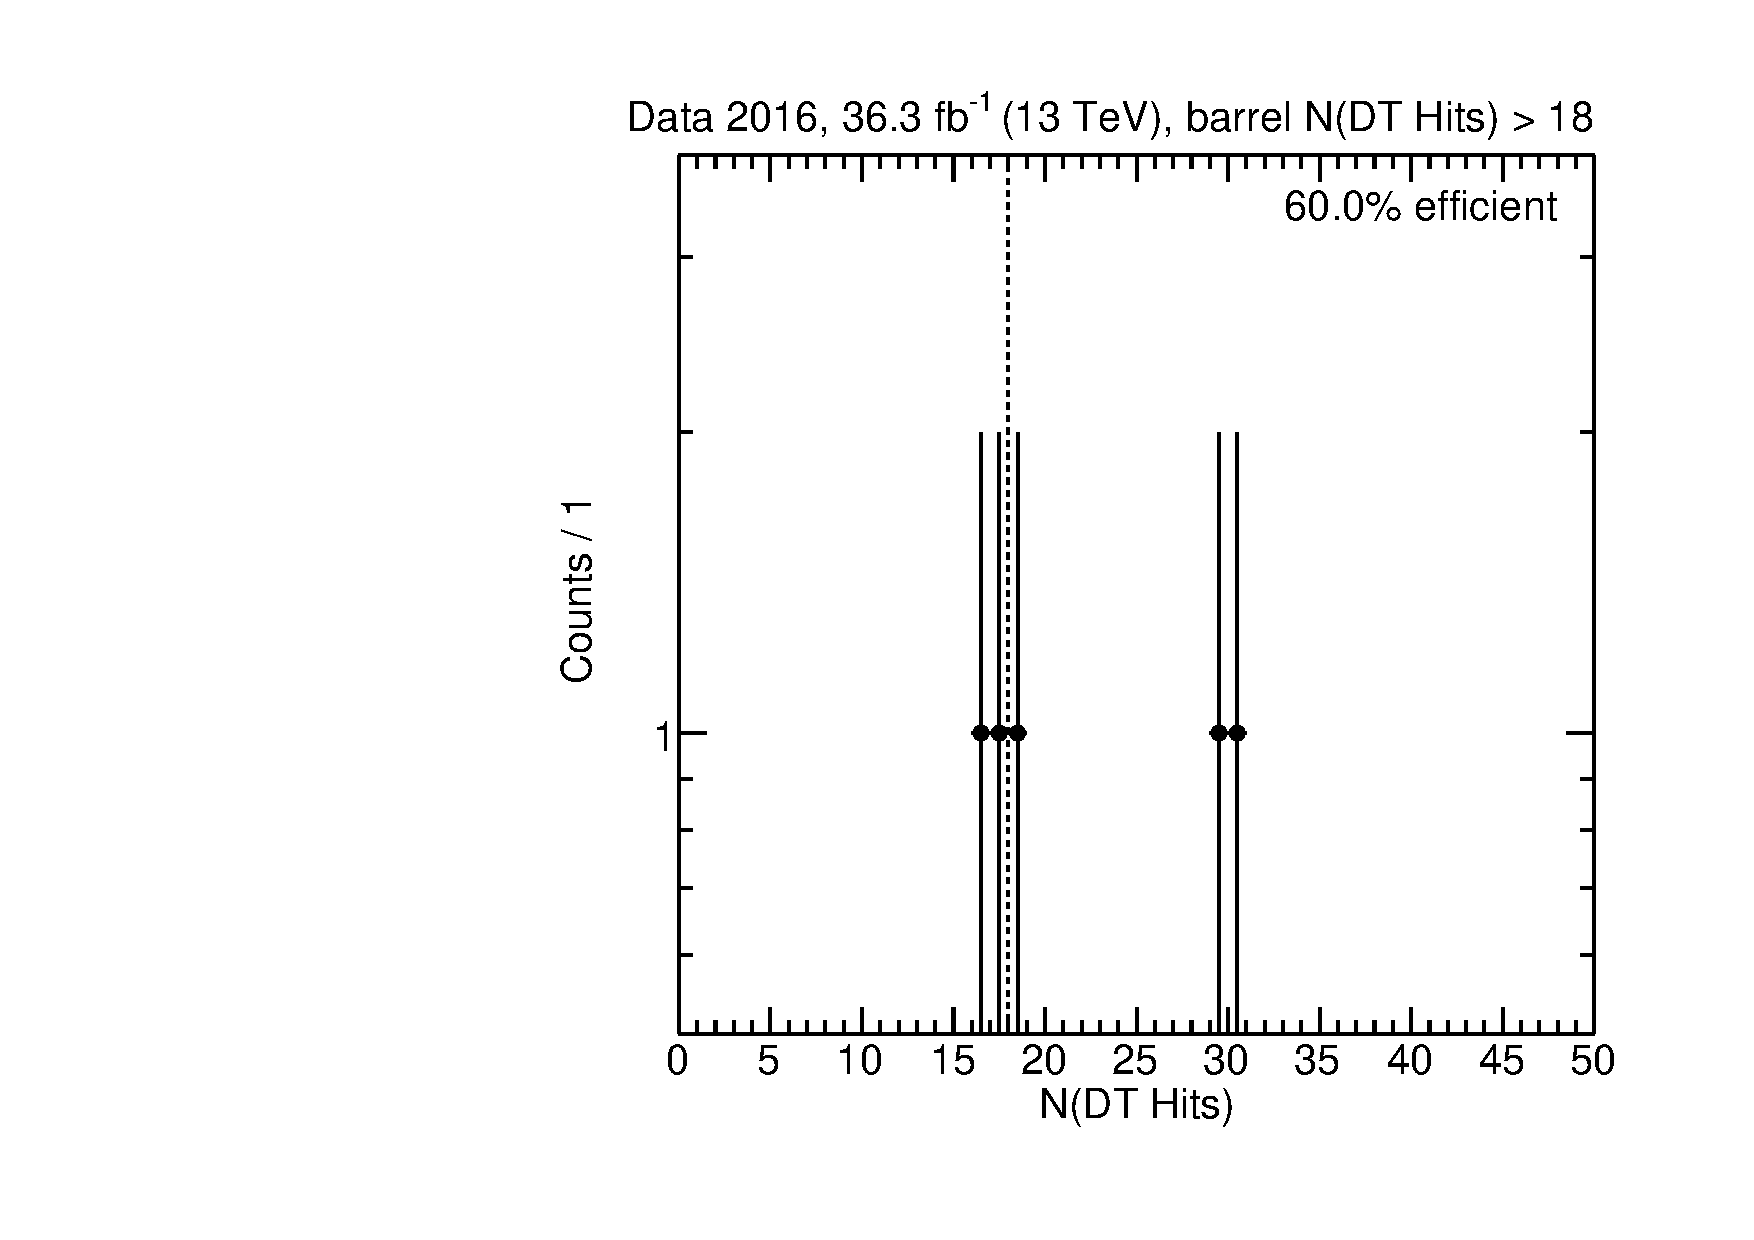
\includegraphics[width=\DSquareWidth]{figures/displaced/NM1_Data_nDTHits.pdf}
  \caption[Histograms of events passing the full selection except for the barrel $N(\text{DT hits})$ cut in \twoMu signal and data.]{Histograms of events passing the full selection except for the barrel $N(\text{DT hits})$ cut, in \figpos{left} \twoMu signal and \figpos{right} data in the control region, along with the labeled cut value (and corresponding dashed line) and the selection efficiency.}
  \label{fig:dd:NM1_nDTHits}
\end{figure}

\begin{figure}[p]
  \centering
  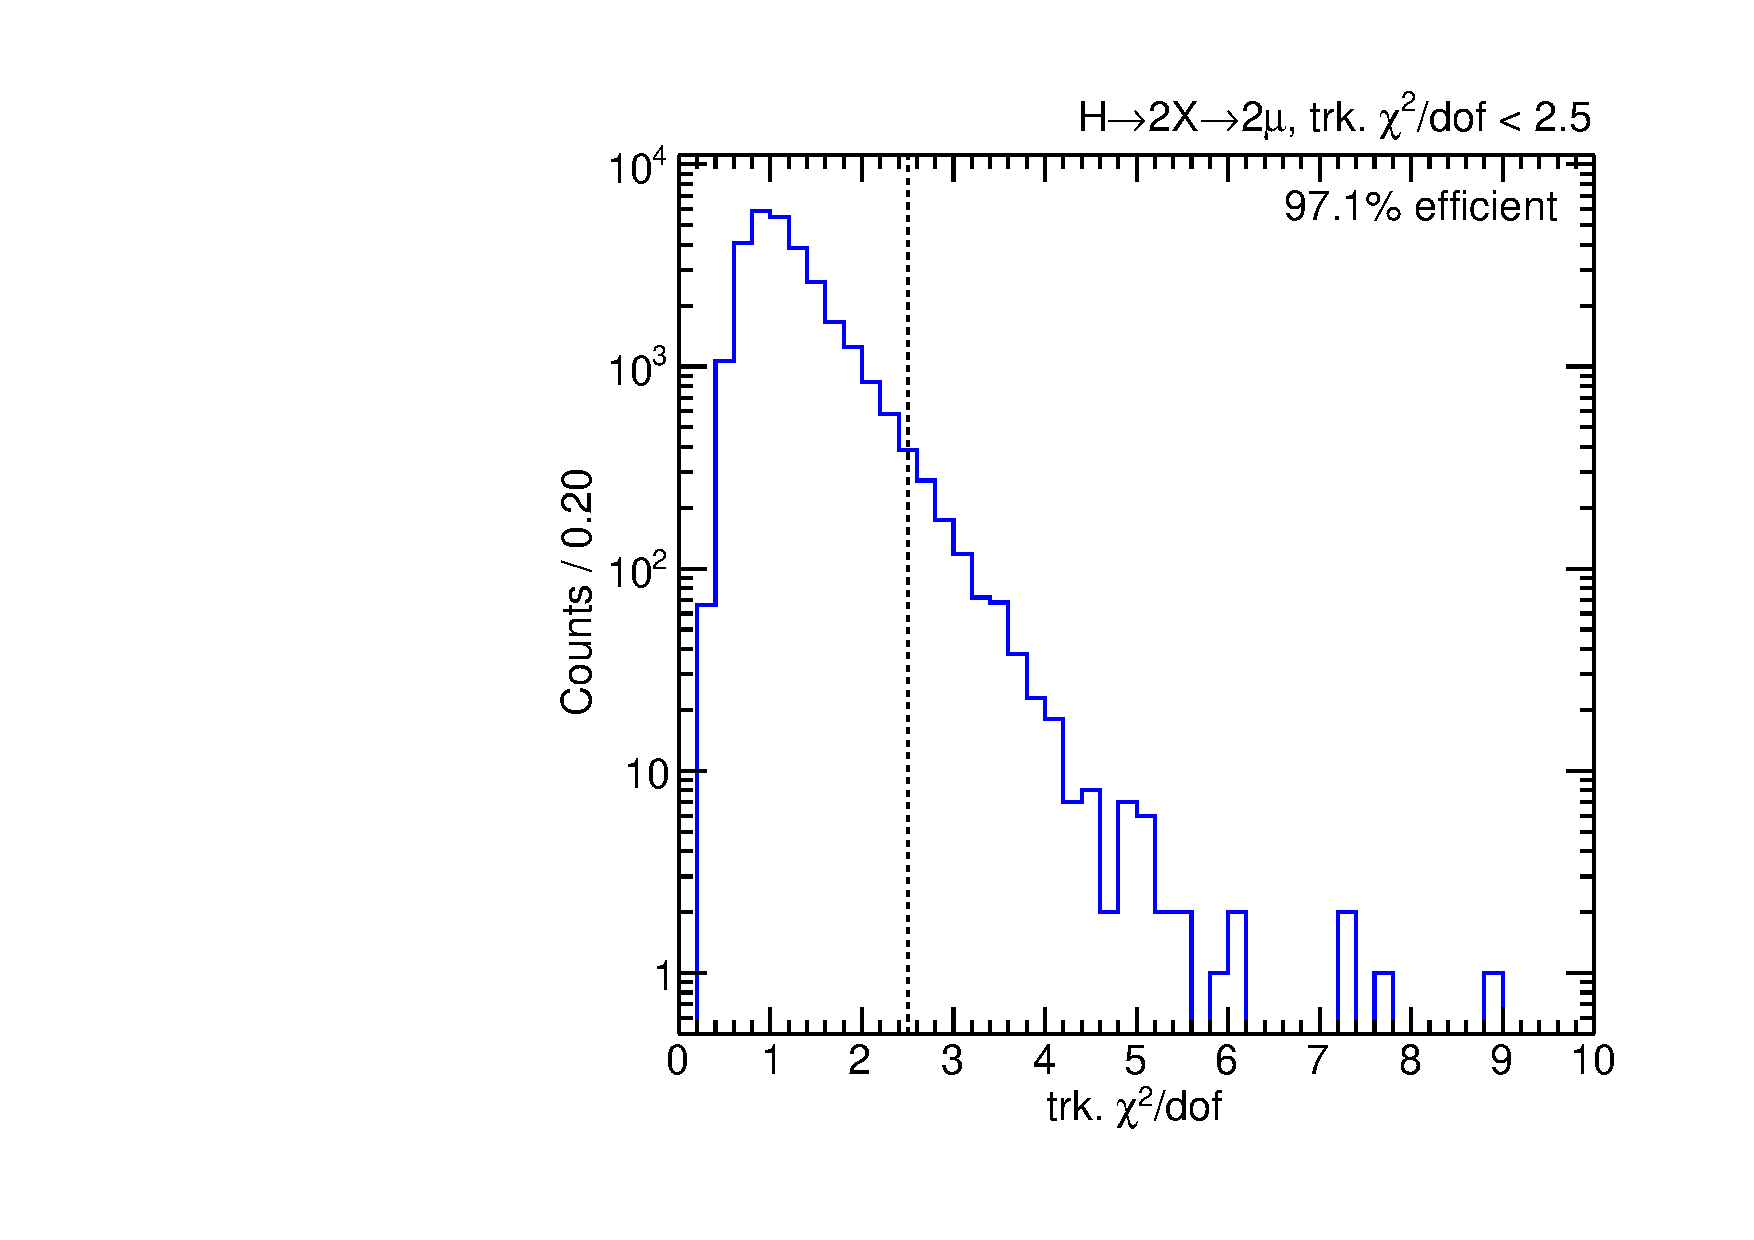
\includegraphics[width=\DSquareWidth]{figures/displaced/NM1_2Mu2J_trkChi2.pdf}
  \hspace*{-2em}
  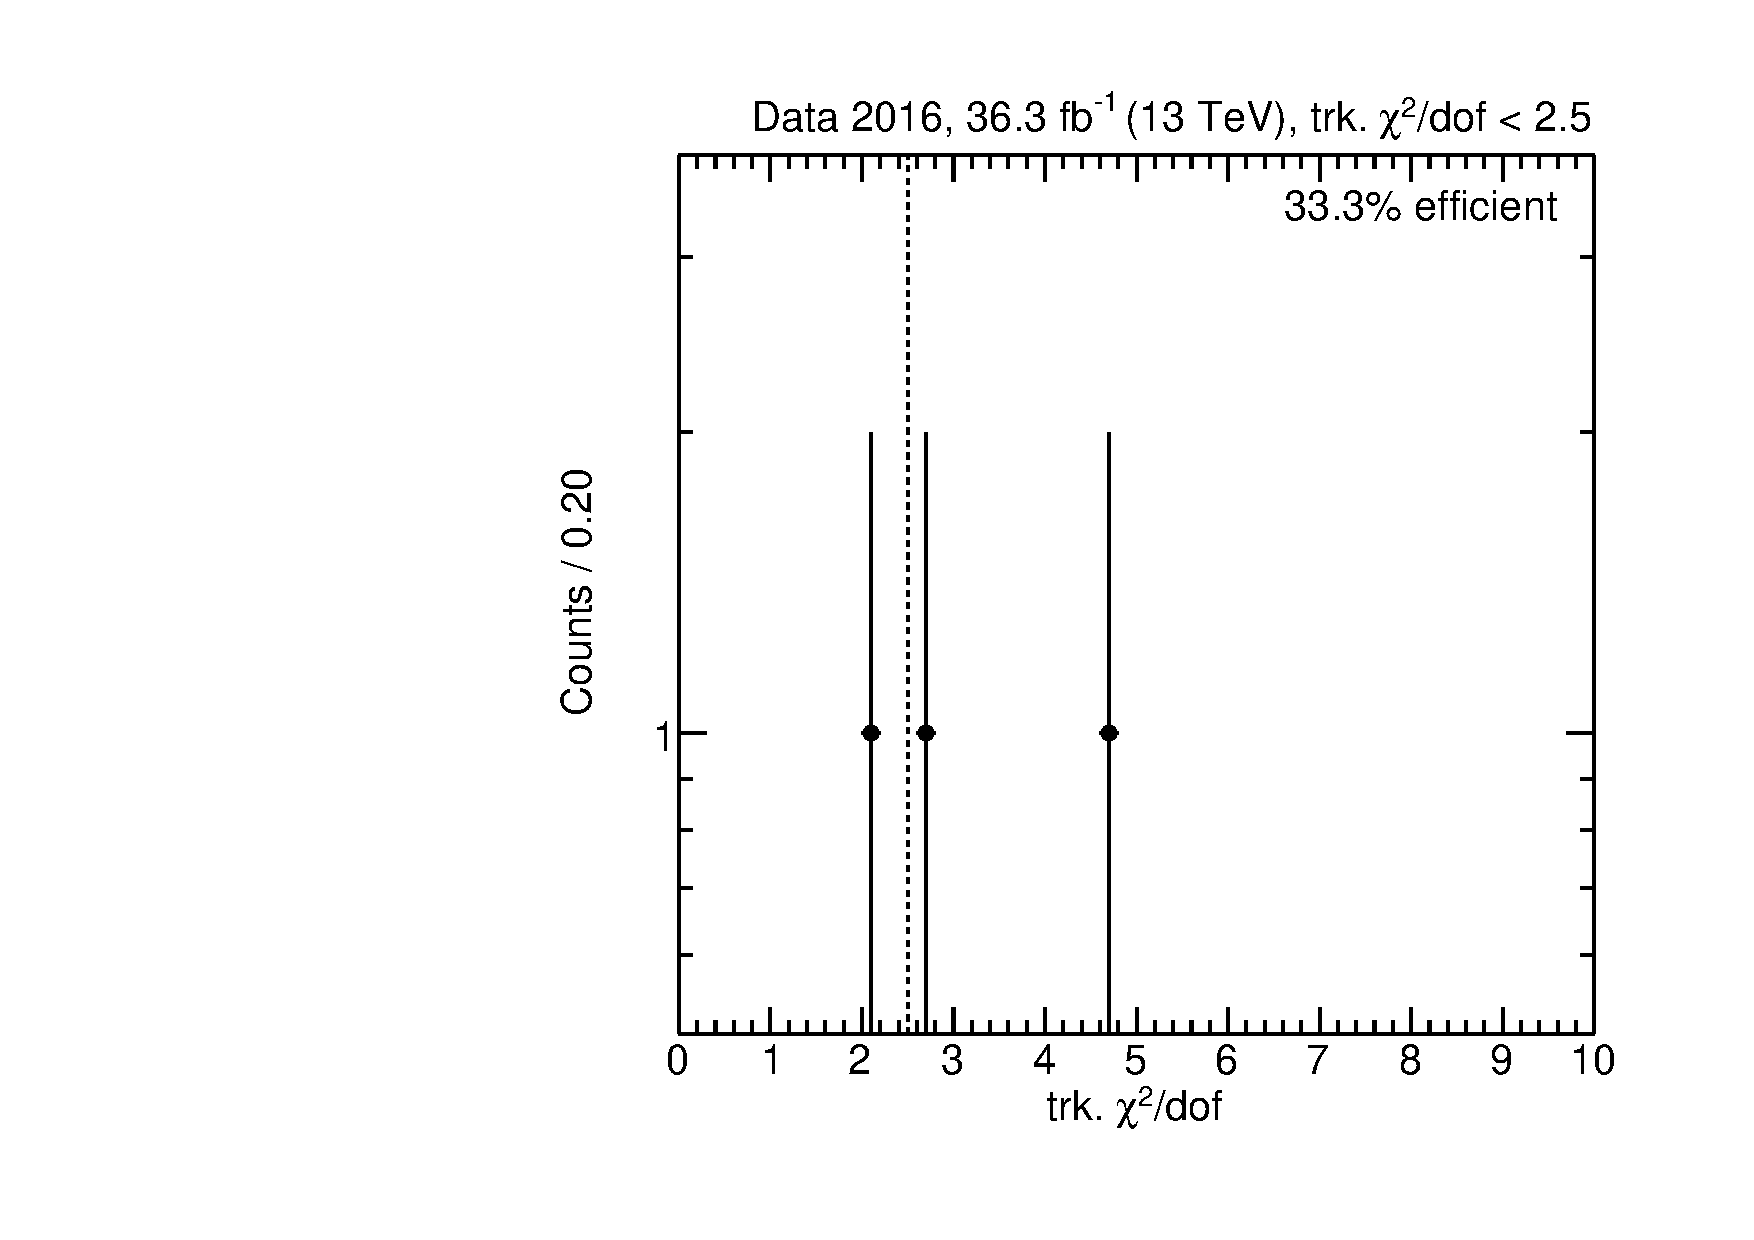
\includegraphics[width=\DSquareWidth]{figures/displaced/NM1_Data_trkChi2.pdf}
  \caption[Histograms of events passing the full selection except for the track \normchisq cut in \twoMu signal and data.]{Histograms of events passing the full selection except for the track \normchisq cut, in \figpos{left} \twoMu signal and \figpos{right} data in the control region, along with the labeled cut value (and corresponding dashed line) and the selection efficiency.}
  \label{fig:dd:NM1_trkChi2}
\end{figure}

\begin{figure}[p]
  \centering
  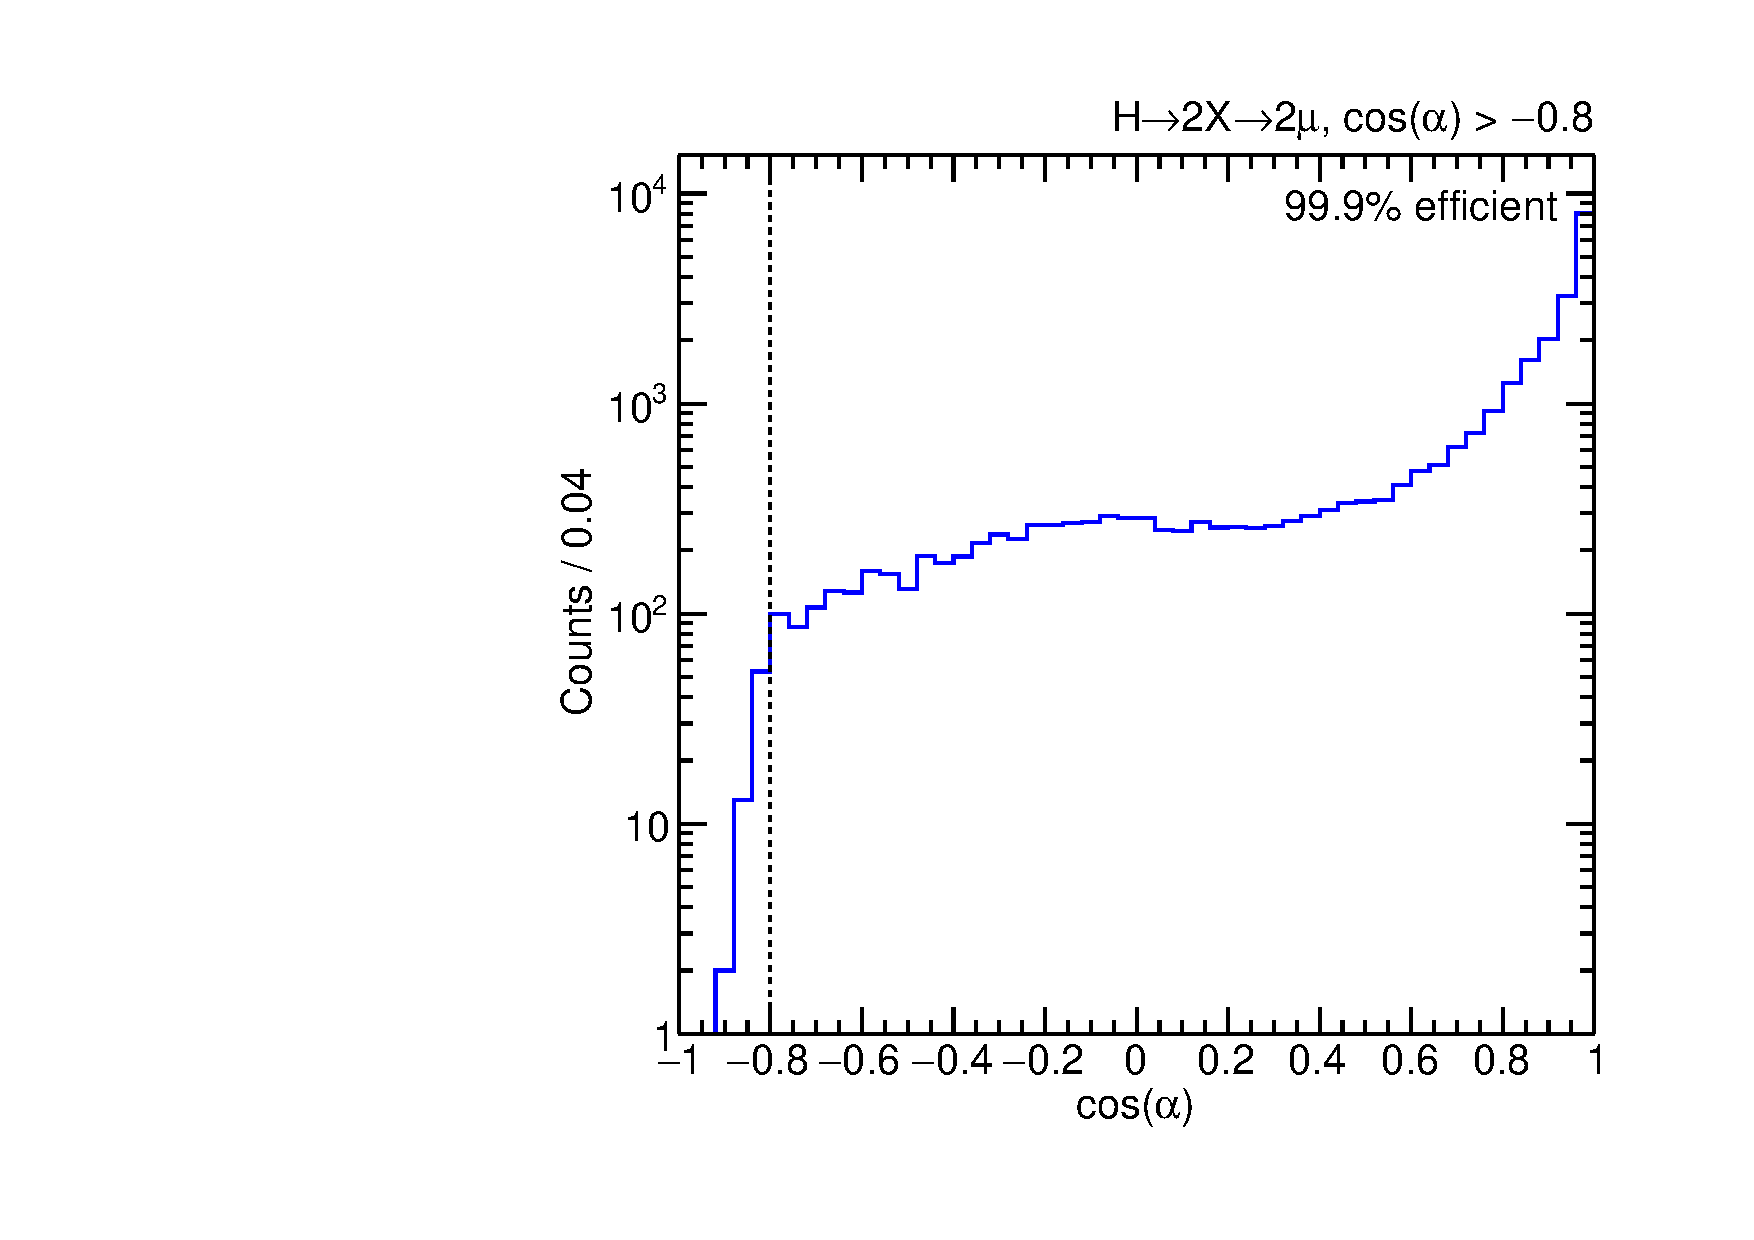
\includegraphics[width=\DSquareWidth]{figures/displaced/NM1_2Mu2J_cosAlpha.pdf}
  \hspace*{-2em}
  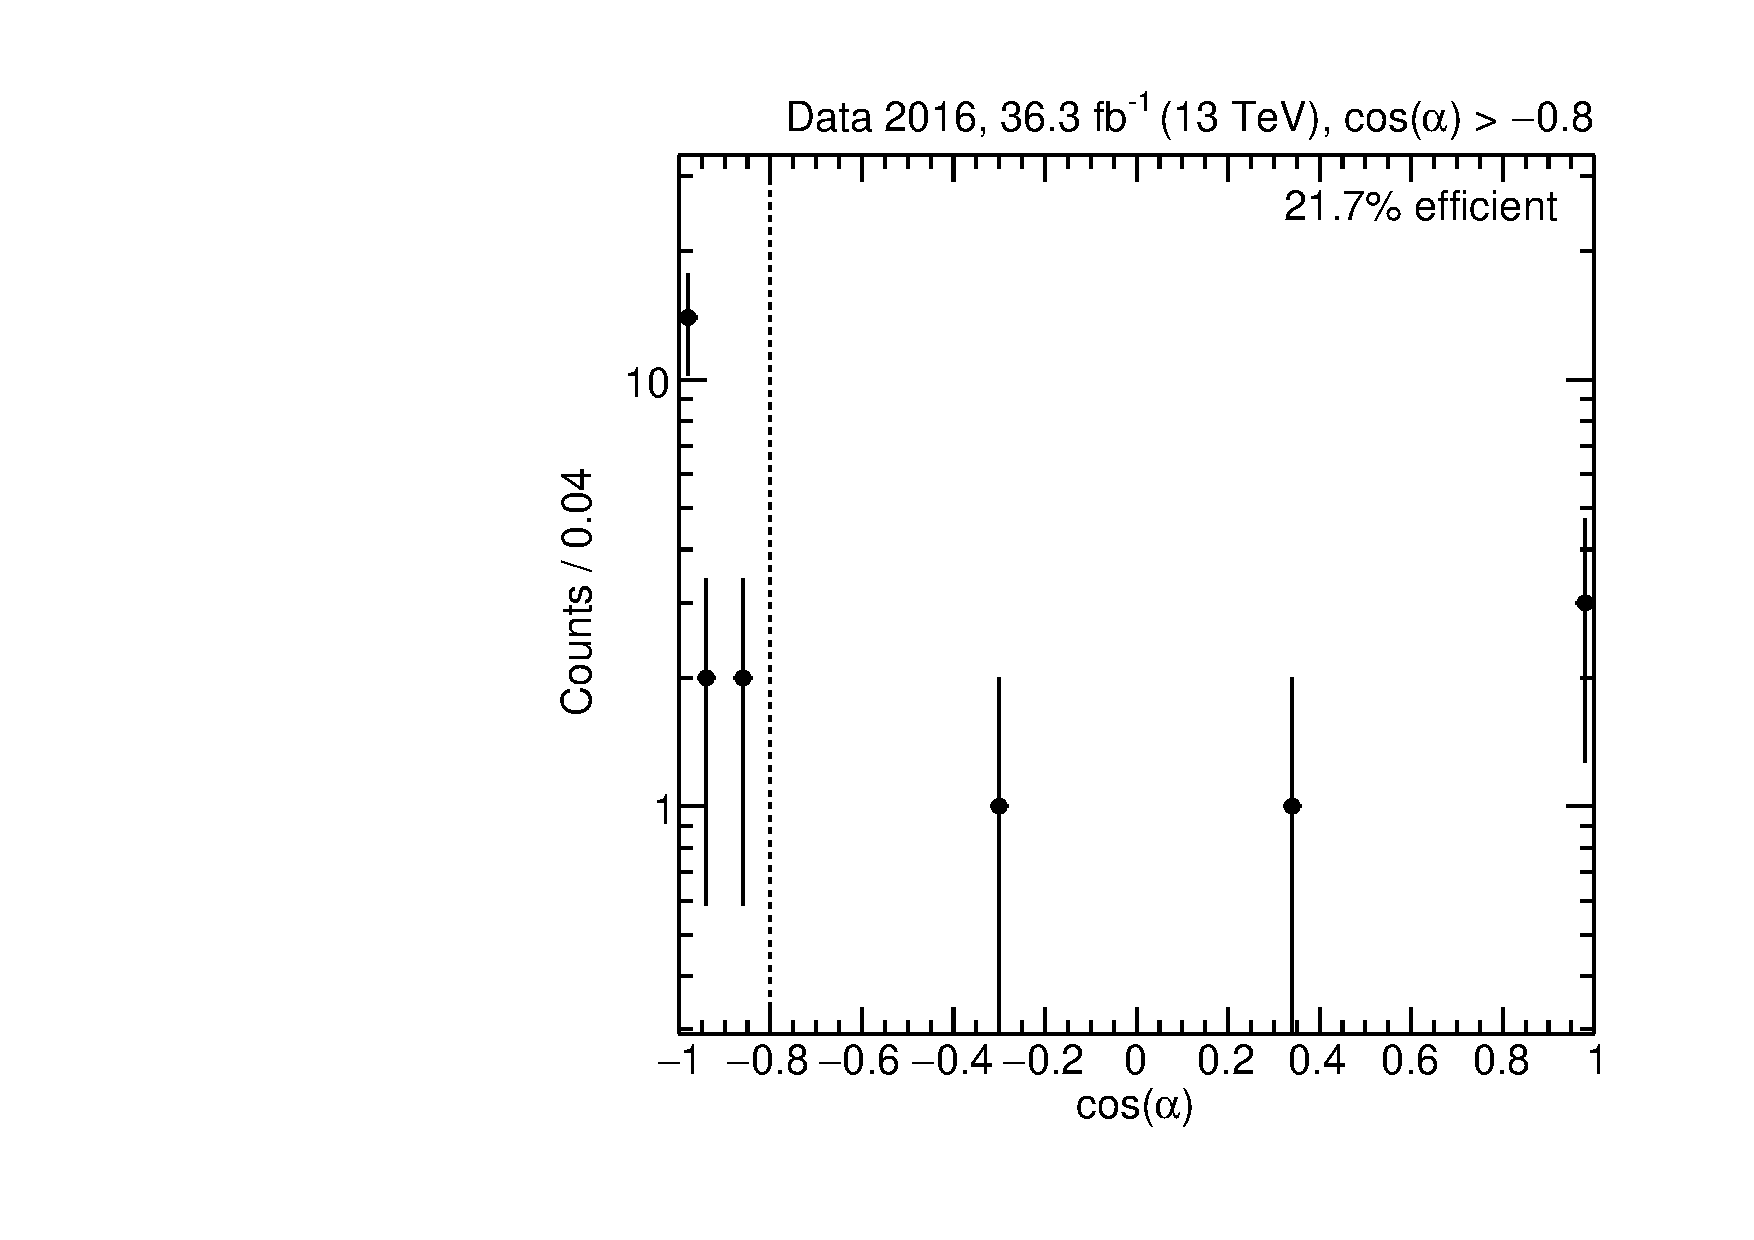
\includegraphics[width=\DSquareWidth]{figures/displaced/NM1_Data_cosAlpha.pdf}
  \caption[Histograms of events passing the full selection except for the $\cos{\alpha}$ and $N$(parallel pairs) cuts in \twoMu signal and data.]{Histograms of events passing the full selection except for the $\cos{\alpha}$ and $N$(parallel pairs) cuts, in \figpos{left} \twoMu signal and \figpos{right} data in the control region, along with the labeled cut value (and corresponding dashed line) and the selection efficiency.}
  \label{fig:dd:NM1_cosAlpha}
\end{figure}

\begin{figure}[p]
  \centering
  \includegraphics[width=\DSquareWidth]{figures/displaced/NM1_2Mu2J_Npp.pdf}
  \hspace*{-2em}
  \includegraphics[width=\DSquareWidth]{figures/displaced/NM1_Data_Npp.pdf}
  \caption[Histograms of events passing the full selection except for the $\cos{\alpha}$ and $N$(parallel pairs) cuts in \twoMu signal and data.]{Histograms of events passing the full selection except for the $\cos{\alpha}$ and $N$(parallel pairs) cuts, in \figpos{left} \twoMu signal and \figpos{right} data in the control region, along with the labeled cut value (and corresponding dashed line) and the selection efficiency.}
  \label{fig:dd:NM1_Npp}
\end{figure}

\begin{figure}[p]
  \centering
  \includegraphics[width=\DSquareWidth]{figures/displaced/NM1_2Mu2J_vtxChi2.pdf}
  \hspace*{-2em}
  \includegraphics[width=\DSquareWidth]{figures/displaced/NM1_Data_vtxChi2.pdf}
  \caption[Histograms of events passing the full selection except for the vertex \chisq cut in \twoMu signal and data.]{Histograms of events passing the full selection except for the vertex \chisq cut, in \figpos{left} \twoMu signal and \figpos{right} data in the control region, along with the labeled cut value (and corresponding dashed line) and the selection efficiency.}
  \label{fig:dd:NM1_vtxChi2}
\end{figure}

\begin{figure}[p]
  \centering
  \includegraphics[width=\DSquareWidth]{figures/displaced/NM1_2Mu2J_LxySig.pdf}
  \hspace*{-2em}
  \includegraphics[width=\DSquareWidth]{figures/displaced/NM1_Data_LxySig.pdf}
  \caption[Histograms of events passing the full selection except for the \LxySig cut in \twoMu signal and data.]{Histograms of events passing the full selection except for the \LxySig cut, in \figpos{left} \twoMu signal and \figpos{right} data in the control region, along with the labeled cut value (and corresponding dashed line) and the selection efficiency.}
  \label{fig:dd:NM1_LxySig}
\end{figure}

\section{Systematic Uncertainties}
\label{sec:dd:systunc}
This analysis produces an estimated number of signal events, given a signal model, and an estimated number of background events, given the background model.
However, there are uncertainties associated with these estimates arising from a variety of sources; these uncertainties are known as systematic uncertainties, though most are ultimately statistical in origin.
There are three main classes of systematic uncertainties in this analysis: the uncertainty on the measurement of the integrated luminosity, uncertainties associated with the signal estimate, and uncertainties associated with the background estimate.

\pagebreak
\subsection{Luminosity Uncertainty}
The uncertainty on the integrated luminosity for the 2016 data taking period is 2.5\% \cite{CMS-PAS-LUM-17-001}.
This uncertainty directly applies to the signal estimate, as the number of signal events is estimated from Monte Carlo simulation and normalized to compare to the integrated luminosity in data.
However, as the expected background is estimated from data, and not from Monte Carlo simulation, this uncertainty does not apply to the estimated background.

\subsection{Background Uncertainties}
\label{sec:dd:bgunc}
The values of the transfer factors obtained in \Sec~\ref{sec:dd:bgest} were computed with somewhat arbitrary choices (\eg for \LxySig windows) and with assumptions that the values obtained from various control regions were relevant for estimating the background in the signal region.
The associated uncertainties are expected to be the largest systematic uncertainties in the background estimation (though still smaller than uncertainties that are statistical in origin).

The value of the Drell-Yan background transfer factor varies within 2-7\% as reasonable variations are made in the value of relative isolation satisfied by the PAT muons, in the \LxySig values satisfied by the matched PAT dimuons, or across the mass windows containing the \PZ\ mass peak enumerated in \Tab~\ref{tab:dd:masswindow}.
As the final results of the analysis are robust with respect to the assigned uncertainty, it is reasonable to assign a slightly larger number, a systematic uncertainty of 10\%, to the Drell-Yan transfer factor $\TF_\text{DY}$.

The value of the QCD background transfer factor is dominated by statistical uncertainties arising from the small numbers of events used to estimate it.
Changes to the value of the relative isolation satisfied by the PAT muons and to the the \LxySig values satisfied by the matched PAT dimuons have a small effect in comparison.
Moreover, the value is found to depend on the mass windows, with larger values close to 10\GeV.
The values of the QCD transfer factors are therefore given for each mass window, with the systematic uncertainty defined to be the statistical uncertainty obtained by error propagation of the ratio of two Poisson counts used to estimate each factor.
\Tab~\ref{tab:dd:QCDSystUnc} enumerates the QCD transfer factors by mass window, along with each uncertainty.

\begin{table}
  \centering
  \begin{tabular}{lrrll}
    \hline
    Mass Window & \CR[SS]{QCD}{>6}{0} & \CR[OS]{QCD}{>6}{0} & $\tau_\text{QCD}$ & $\sigma_{\TF_\text{QCD}}$ \\
    \hline
    $10\GeV < \mMuMu < 32\GeV$   & 103 & 302         & $2.9 \pm 0.3$  & 11\% \\
    $20\GeV < \mMuMu < 80\GeV$   & 35  & 51          & $1.5 \pm 0.3$  & 22\% \\
    $35\GeV < \mMuMu < 245\GeV$  & 10  & 18          & $1.8 \pm 0.7$  & 39\% \\
    $65\GeV < \mMuMu$            & 3   & 7           & $2.3 \pm 1.6$  & 69\% \\
    Total                        & 115 & 323         & $2.8 \pm 0.9$  & 11\% \\
    \hline
  \end{tabular}
  \caption{Transfer factors $\TF_\text{QCD}$ for estimating QCD background, along with their systematic uncertainties, given in dimuon mass windows.}
  \label{tab:dd:QCDSystUnc}
\end{table}

Events in data with $\LxySig < 6$ are used to cross check these transfer factors.
The histograms of events with $\LxySig < 6$ in the $\DeltaPhi > 3\pi/4$ region are scaled according to transfer factors obtained from the histograms for estimating Drell-Yan background and QCD background.
These plots are given in \Fig~\ref{fig:dd:TFLess}.
\begin{itemize}
  \item The top left plot of \Fig~\ref{fig:dd:TFLess} shows the events passing the full selection in data for $\CR{\Full}{<6}{0}$ (labeled ``SR'', colored red) and for $\CR{\Full}{<6}{\pi}$ (labeled ``CR'', colored blue), showing general agreement between the $\DeltaPhi < \pi/4$ and $\DeltaPhi > 3\pi/4$ regions.
  \item The binwise ratio of the \CR{DY}{<6}{0} and \CR{DY}{<6}{\pi} histograms gives a weight factor for each \LxySig bin; binwise scaling \CR{\Full}{<6}{\pi} by these weights gives the top right plot of \Fig~\ref{fig:dd:TFLess}, with the modified histogram labeled ``CR w/ DY'' and colored green, to represent a correction by the Drell-Yan transfer factor.
  \item The binwise ratio of the \CR[SS]{QCD}{<6}{0} and \CR[OS]{QCD}{<6}{0} histograms gives a weight factor for each \LxySig bin; binwise scaling the 4 events in \CR[SS]{\Full}{<6}{0} by these weights and adding them to the modified \CR{\Full}{<6}{\pi} histogram in the top right plot gives the bottom left plot of \Fig~\ref{fig:dd:TFLess}, with the modified histogram labeled ``CR w/ DY+QCD'' and colored violet, to represent a correction by both the Drell-Yan transfer factor and the QCD transfer factor.
  \item All four histograms are plotted together in the bottom right plot of \Fig~\ref{fig:dd:TFLess} for comparison.
\end{itemize}

\begin{figure}[htbp]
  \centering
  \includegraphics[width=\DSquareWidth]{figures/displaced/BGEST_smallLxySig_CR.pdf}
  \hspace*{-2em}
  \includegraphics[width=\DSquareWidth]{figures/displaced/BGEST_smallLxySig_CR_Corr.pdf} \\
  \includegraphics[width=\DSquareWidth]{figures/displaced/BGEST_smallLxySig_CR_Corr_SS.pdf}
  \hspace*{-2em}
  \includegraphics[width=\DSquareWidth]{figures/displaced/BGEST_smallLxySig.pdf}
  \caption{Histograms of \CR{\Full}{<6}{0} and \CR{\Full}{<6}{\pi} in data, with the latter binwise scaled by Drell-Yan and QCD transfer factors, demonstrating agreement and validating the method of obtaining background estimates in the signal region with transfer factors from control regions.}
  \label{fig:dd:TFLess}
\end{figure}
\clearpage

With the exception of a presumed fluctuation in the last bin with a large uncertainty, the corrected ``CR w/ DY+QCD'' histogram (violet) is within error bars of the SR histogram, verifying that the use of the transfer factors to obtain estimates of background events in the signal region is consistent.

\subsection{Signal Uncertainties}
\subsubsection{Signal Lifetime Reweighting}
\label{sec:dd:lifetimereweighting}
As enumerated in \Tab~\ref{tab:dd:signalsamples}, for a given BSM Higgs mass and long-lived particle mass \mH and \mX, this analysis simulated and produced signal samples for only three distinct values of \cTau.
To calculate an estimated number of signal events for lifetimes other than these three nominal lifetimes, this analysis employs a procedure to reweight one signal lifetime into another.
A particle with lifetime $\tau$ will decay after a time $t$ given by a decaying exponential probability distribution $\pazocal{P}(t; \tau) = e^{-t/\tau}/\tau$.
A sample with a decay time distribution of reference lifetime $\tau_\text{ref}$ can be reweighted so that it is distributed with a new lifetime $\tau_\text{new}$ by multiplying the contribution of each event by a weight factor given by the ratio of the two distributions:
\begin{equation}
  w_{\tau_\text{ref}\to\tau_\text{new}}(t) \equiv \frac{\pazocal{P}(t; \tau_\text{new})}{\pazocal{P}(t; \tau_\text{ref})} = \frac{\frac{1}{\tau_\text{new}}e^{-t/\tau_\text{new}}}{\frac{1}{\tau_\text{ref}}e^{-t/\tau_\text{ref}}}
  \label{eq:dd:lifetimereweight}
\end{equation}
where $t$ can be computed from the generated values of suitable experimental quantities in a number of equivalent ways, including
\begin{equation}
  t = \frac{\Lxy}{\mX \cdot \pT^\PLLP}
  \label{eq:dd:decaytime}
\end{equation}
When reweighting from longer (shorter) lifetimes to shorter (longer) lifetimes, events with short decay times are given large (small) weights and events with long decay times are given small (large) weights such that the reference decay time distribution (with unit area) is transformed into the new decay time distribution (also with unit area).

Let the number of generated signal events be $N_\text{gen}$, and let $S$ be the subset of those $N_\text{gen}$ events that pass the trigger and the full selection.
With event weights, the estimated number of passing events $N_\text{pass}$ is
\begin{equation}
  N_\text{pass} = \sum_{i\in S}{w_{\tau_\text{ref}\to\tau_\text{new}}(t_i)}
  \label{eq:dd:npass}
\end{equation}
In the limit of large numbers of events, the sum of the event weights (for all generated events) for the reference and new lifetimes should be equal and equivalent to $N_\text{gen}$.
In practice, instabilities associated with limited sample sizes and large weights generally result in
\begin{equation}
  \sum_{i = 0}^{N_\text{gen}}{w_{\tau_\text{ref}\to\tau_\text{new}}(t_i)} < N_\text{gen}
\end{equation}
It is undesirable for the signal efficiency to suffer from the effect of this underestimated denominator, and so we are prompted to divide $N_\text{pass}$ instead by the true number of generated events, rather than the sum of the weights.
Thus, the signal selection efficiency is defined as
\begin{equation}
  \varepsilon = \frac{N_\text{pass}}{N_\text{gen}}
  \label{eq:dd:signaleff}
\end{equation}
Because the denominator of $\varepsilon$ is an exactly known quantity, the binomial Clopper-Pearson interval does not apply to estimating the uncertainty on $\varepsilon$; only the uncertainty on $N_\text{pass}$ affects the uncertainty on $\varepsilon$.
The uncertainty on the contribution of the $i$th event is its weight, $w_i$.
Treating each uncertainty as independent and uncorrelated, the uncertainty on the sum of all the passing events is obtained from the linear approximation to the propagation of uncertainty:
\begin{equation}
  \sigma_{N_\text{pass}} = \sqrt{\sum_{i\in S}{w_{\tau_\text{ref}\to\tau_\text{new}}(t_i)^2}}
  \label{eq:dd:npassunc}
\end{equation}
This expression reduces to the Poisson uncertainty on the number of passing events $\sqrt{N_\text{pass}}$ when the weights are all 1, \ie without any lifetime reweighting.
It therefore also accounts for the statistical uncertainty arising from estimating an efficiency from a finite sample of events.
The relative uncertainty on $\varepsilon$ can then be defined as the ratio
\begin{equation}
  \frac{\sigma_\varepsilon}{\varepsilon} = \frac{\sigma_{N_\text{pass}}}{N_\text{pass}}
  \label{eq:dd:signaleffunc}
\end{equation}
For the signal samples (nominally, without lifetime reweighting) for which the analysis selection gives non-negligible efficiency (which are the medium and long lifetime samples), the relative uncertainty (which is due to statistical uncertainty only) is 2--5\%.
The uncertainty due to lifetime reweighting increases when reweighting the short and medium lifetime samples to much smaller lifetimes (for which the analysis selection gives negligible efficiency) and when reweighting the short and medium lifetime samples to longer lifetimes (because there are not enough events at intermediate lifetimes to sufficiently estimate the efficiency, and what events there are have large weights).
For the purposes of calculating upper limits, the relative uncertainty (\Eq~\ref{eq:dd:signaleffunc}) is computed for each (reweighted and nominal) signal sample and taken as a systematic uncertainty on the estimated number of signal events.
Any signal estimates with relative uncertainty greater than 50\% are omitted from the calculations.

\subsubsection{Pileup Reweighting}
\label{sec:dd:pileup}
The mean number of \pp collisions per bunch crossing is a measure of the phenomenon known as pileup.
Events with more pileup produce more particles and more tracks in the tracker and in the muon system, which directly impact \eg the reconstruction efficiencies, or the efficiency to associate DSA muons with PAT muons.
The distribution of pileup is different in data than in simulation, and so the distribution in signal simulation is reweighted to correspond to the observed distribution in data. 
This is performed by producing a binned histogram of the distribution of the number of true (as opposed to reconstructed) primary vertices in each event (an estimate of the pileup) for 2016 data and for signal simulation, scaling the histograms to unit area, and dividing the frequency in each bin of the data distribution by the frequency in each bin of the signal distribution.

\Fig~\ref{fig:dd:pileup} shows the distribution of pileup in data and in simulation.
The black dots are the (normalized) distribution of pileup in CMS data taken in 2016 certified for muon physics.
The red dots are the (normalized) distribution of pileup in all \twoMu signal samples combined.
To confirm that this combined distribution is robust with respect to signal parameters, the orange bands represent the binwise maximum and binwise minimum of all 33 sets of signal parameters.
The right plot of \Fig~\ref{fig:dd:pileup} shows the ratio of the data distribution to the signal distribution(s) in the left plot.
Each bin---corresponding to a number of true primary vertices---now contains the signal event weight.

\begin{figure}[htpb]
  \centering
  \includegraphics[width=\DSquareWidth]{figures/displaced/PU_distributionNom.pdf}
  \hspace*{-2em}
  \includegraphics[width=\DSquareWidth]{figures/displaced/PU_weightNom.pdf}
  \caption[Histograms of the number of true primary vertices in 2016 data and in \twoMu signal, and graph of their ratios.]{\figpos{Left} Histogram of the number of true primary vertices in 2016 data and in \twoMu signal. \figpos{Right} Ratio of the data histogram to the signal histogram, giving the nominal signal event weight for a given number of true primary vertices.}
  \label{fig:dd:pileup}
\end{figure}

To formalize the notation, let $\pazocal{D}(P)$ be the histogram in data (normalized to unit area), and $\pazocal{S}(P)$ be the the histogram for all signal samples combined (normalized to unit area), giving the distribution of pileup $P$.
Let $P(i)$ be the number of true primary vertices in the $i$th simulated signal event.
Then the pileup weight factor for the $i$th signal event is
\begin{equation}
  w_\text{pileup}(P(i)) = \frac{\pazocal{D}(P)}{\pazocal{S}(P)}
  \label{eq:dd:pileupweight}
\end{equation}
and the contribution of each event is scaled by the weight factor.

There is a systematic uncertainty associated with this pileup reweighting procedure arising from an uncertainty in the minimum-bias \pp cross section used to calculate the data pileup distribution; the nominal value of this cross section is 69.2\unit{mb}.
To estimate the effect of this uncertainty, the \pp cross section used to calculate the pileup distribution in data is varied by $\pm 5\%$, and the analysis signal yield is recomputed using the pileup event weights obtained from the upwards variation and downwards variation.
For signal samples for which the analysis selection gives non-negligible efficiency, the variation due to variations in pileup reweighting was found to be 2\% or less for all signal samples.
Therefore, the systematic uncertainty on the signal estimate due to pileup modeling is taken to be 2\%.

The definitions of $N_\text{pass}$, $N_\text{gen}$, and $\sigma_{N_\text{pass}}$ in \Eqs~\ref{eq:dd:npass}--\ref{eq:dd:signaleffunc} are consequently modified to be
\begin{align}
  \label{eq:dd:LRWithPileupA}
  N_\text{pass}          &\to \sum_{i\in S}{\left[w_{\tau_\text{ref}\to\tau_\text{new}}(t_i) \cdot w_\text{pileup}(P(i))\right]} \\
  \label{eq:dd:LRWithPileupB}
  N_\text{gen}           &\to \sum_{i = 0}^{N_\text{gen}}{w_\text{pileup}(P(i))} \\
  \label{eq:dd:LRWithPileupC}
  \sigma_{N_\text{pass}} &\to \sqrt{\sum_{i\in S}{\left[w_{\tau_\text{ref}\to\tau_\text{new}}(t_i) \cdot w_\text{pileup}(P(i))\right]^2}}
\end{align}
As the pileup weights are small compared to the weights due to signal lifetime reweighting, the uncertainty on the modified $N_\text{gen}$ is taken to be negligible, and the procedure for obtaining the uncertainty on the signal estimate due to lifetime reweighting as described in \Sec~\ref{sec:dd:lifetimereweighting} is not modified, except for the definitions in \Eqs~\ref{eq:dd:LRWithPileupA}--\ref{eq:dd:LRWithPileupC}.

\begin{table}
  \centering
  \begin{tabular}{cccc}
    \hline
    Uncertainty                            & Value                     & Signal     & Background \\
    \hline
    Lifetime reweighting                   & 2--50\%                   & \checkmark &            \\
    Luminosity                             & 2.5\%                     & \checkmark &            \\
    Pileup                                 & 2\%                       & \checkmark &            \\
    Trigger efficiency                     & 15\%                      & \checkmark &            \\
    Reconstruction efficiency              & 15\%                      & \checkmark &            \\
    Transfer factor $\TF_\text{DY}$        & 10\%                      &            & \checkmark \\
    Transfer factor $\TF_\text{QCD}$       & 11--69\%                  &            & \checkmark \\
    Statistical \CR{\Full}{>6}{\pi}$\to$SR & see \Sec~\ref{sec:dd:cls} &            & \checkmark \\
    \hline
  \end{tabular}
  \caption[Summary of systematic uncertainties in this analysis for signal and background estimates.]{Summary of systematic uncertainties in this analysis, along with a check mark indicating whether the uncertainty applies to the signal or to the background estimate. As discussed in \Sec~\ref{sec:dd:cls}, the statistical uncertainty due to extrapolating a background estimate in a signal region from a control region is treated specially, and represents the dominant systematic uncertainty for the background estimate.}
  \label{tab:dd:systunc}
\end{table}

\subsubsection{Other Signal Systematic Uncertainties}
The efficiencies of the trigger and of the DSA reconstruction are different in data than in simulation.
Estimating them in data is challenging because a real source of displaced muons is required; a dedicated study for estimating these efficiencies from data using cosmic ray muons with large impact parameters is in progress.
Other than potentially large uncertainties from lifetime reweighting, these systematic uncertainties are expected to be the dominant systematic uncertainties on the estimated signal.
Based on our current understanding, each of the trigger and reconstruction efficiencies are assigned a systematic uncertainty of 15\%.
Other systematic uncertainties, such as theoretical uncertainties from next-to-leading-order modeling and choices of parton distribution functions, are taken to be negligible for this analysis.

\section{Results}
\subsection{Computing Upper Limits with the \CLs Criterion}
\label{sec:dd:cls}
The procedure for setting an upper limit on the long-lived particle production cross section times the branching fraction to two muons is as follows \cite{CMS-NOTE-2011-005}.
Let the probability of obtaining the observed data $x$ be $\pazocal{P}(x; \sigstr, \theta)$ (probability density function, or pdf, if $x$ is continuous).
Here \sigstr is the signal strength, a quantity proportional to the signal cross section, so that $\sigstr = 0$ represents a background-only model, and $\theta$ represents the systematic uncertainties, also referred to as nuisance parameters.
A model therefore defines an expected number of signal events, an expected number of background events, and a set of systematic uncertainties.
Then the likelihood function for a model with signal strength \sigstr and nuisance parameters $\theta$ given some observed data $x = X$ is $\pazocal{L}\left(\sigstr, \theta \,\vert\, X\right)$.
This likelihood function is globally maximized at some values $\sigstr = \hat{\sigstr}$ and $\theta = \hat{\theta}$, and for a specific value of \sigstr, locally maximized at $\theta = \hat{\hat{\theta}}_\sigstr$.
The LHC-style test statistic \cite{CombineManual} is then defined, based on a ratio of profile likelihoods, as

\begin{equation}
  q_\text{LHC}(\sigstr) = -2\ln\left[\frac{\pazocal{L}\left(\sigstr, \hat{\hat{\theta}}_\sigstr \,\vert\, X\right)}{\pazocal{L}\left(\sigstr = \hat{\sigstr}, \theta=\hat{\theta}\,\vert\,  X\right)}\right]
  \label{eq:dd:qLHC}
\end{equation}
The likelihoods are evaluated following the Cousins-Highland prescription of treating the signal strength in a frequentist manner and incorporating the systematic uncertainties by marginalizing (or integrating over) them (treating them in a Bayesian manner by designating their prior pdfs) \cite{CousinsHighland:SystUnc1992}.

For most types of systematic uncertainties, the prior pdfs are assumed to follow a log-normal distribution, with one exception.
There is a systematic uncertainty on the estimated background associated with the statistical uncertainty arising from estimating the expected background in the signal region from a number of observed events in the control region.
The prior pdf for this systematic uncertainty is assumed to follow a gamma distribution, which has good frequentist properties; from a Bayesian point of view, it is the posterior pdf for the background mean if the prior pdf is uniform and the likelihood function is from one sample of a Poisson distribution \cite{Cousins:ZBi2008, Cousins:LogNormal}.

For some observation $X$, the minimal value $Q(X)$ of the test statistic $q_\text{LHC}(\sigstr)$ corresponds to the value of \sigstr with maximum likelihood.
Then the pdf of the minimal value of the test statistic $\pazocal{P}(Q;\sigstr)$, given a signal strength \sigstr, is computed, by sampling observations $X$ from ensembles of toy experiments generated using Monte Carlo methods, computing the likelihood functions, and minimizing the test statistic.
The actual observation $X_\text{obs}$ in CMS data taken in 2016 corresponds to some minimal value of the test statistic $Q_\text{obs} = Q(X_\text{obs})$.
Define the $p$-values for signal and background as
\begin{align}
  p_\sigstr   &= \int_{-\infty}^{Q_\text{obs}}{\pazocal{P}(Q;\sigstr)\dd{Q}}\\
  1 - p_b     &= \int_{-\infty}^{Q_\text{obs}}{\pazocal{P}(Q;0)      \dd{Q}}
  \label{eq:dd:pvalues}
\end{align}
In the 1990s and decades before, using the standard $p$-value $p_\sigstr$ to place upper limits on \sigstr was known to cause difficulties if there was a severe downward fluctuation in the background.
Three proposed solutions became widely accepted and are described in the PDG Review of Particle Physics statistical section \cite{CowanPDGStats}, namely, the method advocated by Feldman and Cousins; a Bayesian method with priors that are known to give good frequentist coverage or over-coverage; and an invention in high-energy physics known as \CLs.
By convention the ATLAS and CMS collaborations use \CLs \cite{Read:CLs, Junk:CLs} for most results, and this convention is followed here.
It leads to upper limits that over-cover at the stated confidence level, if the statistical model is correct.
This modified frequentist statistic \CLs is defined as
\begin{equation}
  \CLs = \frac{p_\sigstr}{1-p_b}
  \label{eq:CLs}
\end{equation}
For some confidence level $1-\alpha$, signal models with values of \CLs such that $\CLs \leq \alpha$ are excluded at a confidence level of $1-\alpha$.
The 95\% confidence level upper limit on the signal strength $\sigstr_\text{UL}$ is therefore the value of $\sigstr$ such that $\CLs = 0.05$.

\subsection{Technical Details of Using the Higgs Combine Tool}
\label{sec:dd:combine}
The CMS software framework includes a statistical analysis package known as the Higgs Combine tool (or simply \combine) used throughout CMS for computing statistical significance and upper limits and for performing goodness-of-fit tests \cite{CombineManual}.
The choices of statistical methods described above were made because this analysis involves low numbers of events.
These choices result in a technical procedure for using \combine to compute upper limits that differs from that used by many CMS analyses.
For this reason, the procedure and the command-line options to \combine are documented here.

Using \combine begins with providing an expected number of signal events (given a model), an expected number of background events, (nominal) values for the systematic uncertainties along with the functional form of their distributions, and an observed number of events in data.
The \combine program is then run with the following configurations controlling the statistical treatment:
\begin{itemize}
  \item \texttt{--rule CLs}: computes the \CLs upper limit.
  \item \texttt{--cl 0.95}: computes the upper limit at a 95\% confidence level.
  \item \texttt{--method HybridNew}: generates toy experiments to compute the distribution of the test statistic, instead of using the asymptotic frequentist approximations of the distribution valid only for large numbers of events.
  \item \texttt{--toysH 5000}: generates 5000 toy experiments each iteration.
  \item \texttt{--iterations 1}: generates \texttt{toysH} toy experiments 1 time.
  \item \texttt{--seed -1}: randomizes the seed
  \item \texttt{--hintMethod AsymptoticLimits}: estimate the upper limit on the signal strength using asymptotic frequentist methods, and use the result to inform the range of signal strengths over which to search when running toy experiments.
  \item \texttt{--testStat LHC}: compute the distribution of the LHC-style test statistic.
  \item \texttt{--generateNuisances 1 --fitNuisances 0}: treats the nuisance parameters in a Bayesian manner by integrating over them. For each toy experiment, the value of the nuisance parameters are randomized within their pdfs.
  \item \texttt{--expectedFromGrid [QUANTILE]}: computes the \texttt{QUANTILE} quantile of the expected upper limit. When omitted, the program computes the observed limit; otherwise, \texttt{QUANTILE} is 0.5 for the median of the distribution under the background-only hypothesis; 0.16 and 0.84 for the lower and upper edges of the 68\% quantile; and 0.025 and 0.975 for the lower and upper edges of the 95\% quantile. 
\end{itemize}

To provide \combine with an expected number of \twoMu signal events, given a signal model defined by values for \mH, \mX, and \cTau, let
\begin{equation}
  N_s^\text{exp} = \left[\sigma(\PHiggs\to \PLLP\PLLP)B(\PLLP\to\Pgm\Pgm)\right]_\text{ass} \cdot \intlumi \cdot \varepsilon
  \label{eq:dd:nExp}
\end{equation}
where $\varepsilon$ was defined in \Secs~\ref{sec:dd:lifetimereweighting}--\ref{sec:dd:pileup}, and $\left[\sigma(\PHiggs\to \PLLP\PLLP)B(\PLLP\to\Pgm\Pgm)\right]_\text{ass}$ is an assumed arbitrary value of the $\PHiggs\to \PLLP\PLLP$ production cross section times the branching ratio for the decay of the long-lived particle to two muons $\PLLP\to\Pgm\Pgm$.
Then \combine returns $\sigstr_\text{UL}$, which can be interpreted as the ratio of the upper limit on the number of \twoMu signal events to the expected number of \twoMu signal events:
\begin{equation}
  \sigstr_\text{UL} = \frac{N_s^\text{UL}}{N_s^\text{exp}} = \frac{\left[\sigma(\PHiggs\to \PLLP\PLLP)B(\PLLP\to\Pgm\Pgm)\right]_\text{UL} \cdot \intlumi \cdot \varepsilon}{\left[\sigma(\PHiggs\to \PLLP\PLLP)B(\PLLP\to\Pgm\Pgm)\right]_\text{ass} \cdot \intlumi \cdot \varepsilon} = \frac{\left[\sigma(\PHiggs\to \PLLP\PLLP)B(\PLLP\to\Pgm\Pgm)\right]_\text{UL}}{\left[\sigma(\PHiggs\to \PLLP\PLLP)B(\PLLP\to\Pgm\Pgm)\right]_\text{ass}}
  \label{eq:dd:sigmaBfromSigStr}
\end{equation}
Therefore
\begin{equation}
  \left[\sigma(\PHiggs\to \PLLP\PLLP)B(\PLLP\to\Pgm\Pgm)\right]_\text{UL} = \sigstr_\text{UL} \cdot \left[\sigma(\PHiggs\to \PLLP\PLLP)B(\PLLP\to\Pgm\Pgm)\right]_\text{ass}
  \label{eq:dd:sigmaB}
\end{equation}

\subsection{Events Passing the Full Selection Criteria}
\label{sec:dd:eventdisplays}
8 opposite-sign events and 4 same-sign events pass the full selection in 2016 data.
\Tab~\ref{tab:dd:signalregionevents} enumerates these events, with their identifying run, lumi section, and event numbers, and their values of \mMuMu, \DeltaPhi, and \LxySig.
The table also contains references to the event displays for the opposite-sign events in \Figs~\ref{fig:dd:event-944}--\ref{fig:dd:event-501}.
As in \Fig~\ref{fig:dd:shower}, views are presented in both the transverse plane ($\rho$-$\phi$) and the orthogonal $\rho$-$z$ plane.
DSA muon tracks are drawn in yellow (associated segments drawn as yellow dots); PAT muons are drawn in red; jets are drawn in cyan; tracks in the tracker are drawn in gray; missing transverse energy is drawn in purple.
Detailed inspection of the individual events passing all cuts gives no indication that the events are not individually compatible with known backgrounds.
As the numbers of events passing all cuts are compatible with expectations based on the background estimates and the transfer factors, we conclude that no excess is observed.



\subsection{Upper Limits on the Cross Section Times Branching Ratio}
\label{sec:dd:limits}
\Tab~\ref{tab:dd:exp_obs} enumerates the number of opposite-sign events in the control region \CR[OS]{\Full}{>6}{\pi}, the number of same-sign events in the control region \CR[SS]{\Full}{>6}{0}, the corresponding number of expected background events in the signal region, and the number observed events in the signal region, for each mass window in \Tab~\ref{tab:dd:masswindow}, given the events enumerated in \Tab~\ref{tab:dd:signalregionevents}.
Given these observations, the systematic uncertainties described in \Sec~\ref{sec:dd:systunc}, and the procedure described in \Secs~\ref{sec:dd:cls}--\ref{sec:dd:combine}, upper limits on the signal strength for each mass hypothesis are computed and converted to limits on the cross section times the branching ratio.
\Figs~\ref{fig:dd:UpperLimits_mH_1000}--\ref{fig:dd:UpperLimits_mH_125} are plots of the upper limits on $\sigma(\PHiggs\to \PLLP\PLLP)B(\PLLP\to\Pgm\Pgm)$ for various values of BSM Higgs mass \mH and long-lived particle mass \mX as a function of $c$ times the long-lived particle mean proper lifetime \cTau.
In the figure for each limit curve, there is also shown the median upper limit that would be obtained in an imagined ensemble of similar experiments having only background events.
The spread of upper limits about the median in such an ensemble of background-only experiments is indicated by yellow bands containing the central 68\% quantile.
\Tab~\ref{tab:dd:limits} summarizes the values of the median and observed upper limits for the 33 sets of signal parameters (\mH, \mX, \cTau) without any lifetime reweighting.
Some values are omitted, corresponding to signal samples with zero efficiency or statistical uncertainty greater than 50\%.

\begin{table}
  \centering
  \begin{tabular}{lllrrrl}
		\multicolumn{7}{c}{Opposite-Sign Events in $\DeltaPhi < \pi/4$} \\
		\hline
    Run & Lumi & Event & \multicolumn{1}{c}{$\mMuMu\; [\text{GeV}]$} & \multicolumn{1}{c}{\DeltaPhi} & \multicolumn{1}{c}{\LxySig} & Display \\
		\hline
		274969 & 944  & 1675672448 &  10.2 & 0.0764 & 56.91 & \Fig~\ref{fig:dd:event-944} \\
		276935 & 522  & 801995838  &  24.0 & 0.1309 &  6.76 & \Fig~\ref{fig:dd:event-522} \\
		276940 & 97   & 59821031   &  14.8 & 0.1123 & 14.22 & \Fig~\ref{fig:dd:event-97}  \\
		276947 & 4    & 6168006    &  15.4 & 0.0020 &  6.73 & \Fig~\ref{fig:dd:event-4}   \\
		277168 & 114  & 203474554  &  24.6 & 0.0714 & 76.68 & \Fig~\ref{fig:dd:event-114} \\
		278017 & 169  & 188965749  &  64.4 & 0.3114 &  8.90 & \Fig~\ref{fig:dd:event-169} \\
		278308 & 390  & 635154343  & 184.1 & 0.3784 &  8.81 & \Fig~\ref{fig:dd:event-390} \\
		281797 & 501  & 676135274  &  15.6 & 0.0468 & 87.70 & \Fig~\ref{fig:dd:event-501} \\
		\hline \\

		\multicolumn{7}{c}{Same-Sign Events in $\DeltaPhi < \pi/4$} \\
		\hline
    Run & Lumi & Event & \multicolumn{1}{c}{$\mMuMu\; [\text{GeV}]$} & \multicolumn{1}{c}{\DeltaPhi} & \multicolumn{1}{c}{\LxySig} & \\
		\hline
    276935 &  641 & 1009966664 &  32.0 & 0.0327 &  57.6 & \\
    277070 &  717 & 1337738509 &  13.5 & 0.0555 &   6.2 & \\
    278240 &  240 &  484842145 &  10.6 & 0.1733 &  23.6 & \\
    279767 &  774 & 1271651549 &  13.4 & 0.4288 & 106.0 & \\
		\hline \\
  \end{tabular}
  \caption{List of events passing the full selection in 2016 data, with their run, lumi section, and event numbers, the values of \mMuMu, \DeltaPhi, and \LxySig, and the associated event display.}
  \label{tab:dd:signalregionevents}
\end{table}

\begin{table}
  \centering
  \begin{tabular}{lllll}
    \hline
    Dimuon Mass Window           & O.S. in \CR[OS]{\Full}{>6}{\pi} & S.S. in \CR[SS]{\Full}{>6}{0}  & Expected & Observed \\
    \hline
    $10\GeV < \mMuMu < 32\GeV$   & 0                               & 3           &  8.8     & 6        \\
    $20\GeV < \mMuMu < 80\GeV$   & 0                               & 1           &  1.5     & 3        \\
    $35\GeV < \mMuMu < 245\GeV$  & 0                               & 0           &  0.0     & 2        \\
    $65\GeV < \mMuMu$            & 0                               & 0           &  0.0     & 1        \\
    Total                        & 0                               & 4           & 11.2     & 8        \\
    \hline
  \end{tabular}
  \caption[Number of opposite-sign and same-sign events, expected background events, and observed events.]{Number of opposite-sign events in \CR[OS]{\Full}{>6}{\pi}, same-sign events in \CR[SS]{\Full}{>6}{0}, expected background events in SR, and observed events in SR.}
  \label{tab:dd:exp_obs}
\end{table}


\begin{figure}[htpb]
  \centering
  \includegraphics[width=0.6\textwidth]{figures/displaced/event-274969_1675672448_944_RhoPhi.png}
  \includegraphics[width=0.6\textwidth]{figures/displaced/event-274969_1675672448_944_RhoZ.png}
  \caption{Display of $\rho$-$\phi$ and $\rho$-$z$ views of event 1675672448 in 2016 data, in run 274969, lumi section 944.}
  \label{fig:dd:event-944}
\end{figure}

\begin{figure}[htpb]
  \centering
  \includegraphics[width=0.6\textwidth]{figures/displaced/event-276935_801995838_522_RhoPhi.png}
  \includegraphics[width=0.6\textwidth]{figures/displaced/event-276935_801995838_522_RhoZ.png}
  \caption{Display of $\rho$-$\phi$ and $\rho$-$z$ views of event 801995838 in 2016 data, in run 276935, lumi section 522.}
  \label{fig:dd:event-522}
\end{figure}

\begin{figure}[htpb]
  \centering
  \includegraphics[width=0.6\textwidth]{figures/displaced/event-276940_59821031_97_RhoPhi.png}
  \includegraphics[width=0.6\textwidth]{figures/displaced/event-276940_59821031_97_RhoZ.png}
  \caption{Display of $\rho$-$\phi$ and $\rho$-$z$ views of event 59821031 in 2016 data, in run 276940, lumi section 97.}
  \label{fig:dd:event-97}
\end{figure}

\begin{figure}[htpb]
  \centering
  \includegraphics[width=0.6\textwidth]{figures/displaced/event-276947_6168006_4_RhoPhi.png}
  \includegraphics[width=0.6\textwidth]{figures/displaced/event-276947_6168006_4_RhoZ.png}
  \caption{Display of $\rho$-$\phi$ and $\rho$-$z$ views of event 6168006 in 2016 data, in run 276947, lumi section 4.}
  \label{fig:dd:event-4}
\end{figure}

\begin{figure}[htpb]
  \centering
  \includegraphics[width=0.6\textwidth]{figures/displaced/event-277168_203474554_114_RhoPhi.png}
  \includegraphics[width=0.6\textwidth]{figures/displaced/event-277168_203474554_114_RhoZ.png}
  \caption{Display of $\rho$-$\phi$ and $\rho$-$z$ views of event 203474554 in 2016 data, in run 277168, lumi section 114.}
  \label{fig:dd:event-114}
\end{figure}

\begin{figure}[htpb]
  \centering
  \includegraphics[width=0.6\textwidth]{figures/displaced/event-278017_188965749_169_RhoPhi.png}
  \includegraphics[width=0.6\textwidth]{figures/displaced/event-278017_188965749_169_RhoZ.png}
  \caption{Display of $\rho$-$\phi$ and $\rho$-$z$ views of event 188965749 in 2016 data, in run 278017, lumi section 169.}
  \label{fig:dd:event-169}
\end{figure}

\begin{figure}[htpb]
  \centering
  \includegraphics[width=0.6\textwidth]{figures/displaced/event-278308_635154343_390_RhoPhi.png}
  \includegraphics[width=0.6\textwidth]{figures/displaced/event-278308_635154343_390_RhoZ.png}
  \caption{Display of $\rho$-$\phi$ and $\rho$-$z$ views of event 635154343 in 2016 data, in run 278308, lumi section 390.}
  \label{fig:dd:event-390}
\end{figure}

\begin{figure}[htpb]
  \centering
  \includegraphics[width=0.6\textwidth]{figures/displaced/event-281797_676135274_501_RhoPhi.png}
  \includegraphics[width=0.6\textwidth]{figures/displaced/event-281797_676135274_501_RhoZ.png}
  \caption{Display of $\rho$-$\phi$ and $\rho$-$z$ views of event 676135274 in 2016 data, in run 281797, lumi section 501.}
  \label{fig:dd:event-501}
\end{figure}

\begin{figure}[htbp]
  \centering
  \includegraphics[width=\DSquareWidth]{figures/displaced/Limits_2Mu_1000_350_HybridNew.pdf}
  \hspace*{-2em}
  \includegraphics[width=\DSquareWidth]{figures/displaced/Limits_2Mu_1000_150_HybridNew.pdf} \\
  \includegraphics[width=\DSquareWidth]{figures/displaced/Limits_2Mu_1000_50_HybridNew.pdf}
  \hspace*{-2em}
  \includegraphics[width=\DSquareWidth]{figures/displaced/Limits_2Mu_1000_20_HybridNew.pdf} \\
  \caption[95\% CL upper limits on $\sigma(\PHiggs\to \PLLP\PLLP)B(\PLLP\to\Pgm\Pgm)$ for $\mH = 1000\GeV$ for various values of \mX.]{95\% CL upper limits on $\sigma(\PHiggs\to \PLLP\PLLP)B(\PLLP\to\Pgm\Pgm)$ for $\mH = 1000\GeV$ for various values of \mX. Black dots are observed limits; the blue line represents the median expected limits; the yellow shaded bands show the central 68\% quantile.}
  \label{fig:dd:UpperLimits_mH_1000}
\end{figure}

\begin{figure}[htbp]
  \centering
  \includegraphics[width=\DSquareWidth]{figures/displaced/Limits_2Mu_400_150_HybridNew.pdf}
  \hspace*{-2em}
  \includegraphics[width=\DSquareWidth]{figures/displaced/Limits_2Mu_400_50_HybridNew.pdf} \\
  \includegraphics[width=\DSquareWidth]{figures/displaced/Limits_2Mu_400_20_HybridNew.pdf}
  \caption[95\% CL upper limits on $\sigma(\PHiggs\to \PLLP\PLLP)B(\PLLP\to\Pgm\Pgm)$ for $\mH = 400\GeV$ for various values of \mX.]{95\% CL upper limits on $\sigma(\PHiggs\to \PLLP\PLLP)B(\PLLP\to\Pgm\Pgm)$ for $\mH = 400\GeV$ for various values of \mX. Black dots are observed limits; the blue line represents the median expected limits; the yellow shaded bands show the central 68\% quantile.}
  \label{fig:dd:UpperLimits_mH_400}
\end{figure}

\begin{figure}[htbp]
  \centering
  \includegraphics[width=\DSquareWidth]{figures/displaced/Limits_2Mu_200_50_HybridNew.pdf}
  \hspace*{-2em}
  \includegraphics[width=\DSquareWidth]{figures/displaced/Limits_2Mu_200_20_HybridNew.pdf}
  \caption[95\% CL upper limits on $\sigma(\PHiggs\to \PLLP\PLLP)B(\PLLP\to\Pgm\Pgm)$ for $\mH = 200\GeV$ for various values of \mX.]{95\% CL upper limits on $\sigma(\PHiggs\to \PLLP\PLLP)B(\PLLP\to\Pgm\Pgm)$ for $\mH = 200\GeV$ for various values of \mX. Black dots are observed limits; the blue line represents the median expected limits; the yellow shaded bands show the central 68\% quantile.}
  \label{fig:dd:UpperLimits_mH_200}
\end{figure}

\begin{figure}[htbp]
  \centering
  \includegraphics[width=\DSquareWidth]{figures/displaced/Limits_2Mu_125_50_HybridNew.pdf}
  \hspace*{-2em}
  \includegraphics[width=\DSquareWidth]{figures/displaced/Limits_2Mu_125_20_HybridNew.pdf}
  \caption[95\% CL upper limits on $\sigma(\PHiggs\to \PLLP\PLLP)B(\PLLP\to\Pgm\Pgm)$ for $\mH = 125\GeV$ for various values of \mX.]{95\% CL upper limits on $\sigma(\PHiggs\to \PLLP\PLLP)B(\PLLP\to\Pgm\Pgm)$ for $\mH = 125\GeV$ for various values of \mX. Black dots are observed limits; the blue line represents the median expected limits; the yellow shaded bands show the central 68\% quantile.}
  \label{fig:dd:UpperLimits_mH_125}
\end{figure}

\begin{table}
  \renewcommand{\arraystretch}{0.75}
  \centering
  \begin{tabular}{lllll}
    \hline
    \mH (\GeVns) & \mX (\GeVns) & \cTau (\mm) & Expected $[\sigma B]_\text{UL}$ [pb] & Observed $[\sigma B]_\text{UL}$ [pb] \\
    \hline
    \multirow{3}{*}{1000}  & \multirow{3}{*}{350} & 35   & $4.55 \times 10^{-2}$ & $3.65 \times 10^{-2}$ \\
                           &                      & 350  & $2.08 \times 10^{-3}$ & $1.69 \times 10^{-3}$ \\
                           &                      & 3500 & $3.31 \times 10^{-3}$ & $3.04 \times 10^{-3}$ \\
    \hline
    \multirow{3}{*}{1000}  & \multirow{3}{*}{150} & 10   & $2.84 \times 10^{-1}$ & $2.84 \times 10^{-1}$ \\
                           &                      & 100  & $3.07 \times 10^{-3}$ & $3.13 \times 10^{-3}$ \\
                           &                      & 1000 & $2.04 \times 10^{-3}$ & $2.07 \times 10^{-3}$ \\
    \hline
    \multirow{3}{*}{1000}  & \multirow{3}{*}{ 50} & 4    & -        & -                                  \\
                           &                      & 40   & $4.91 \times 10^{-3}$ & $4.92 \times 10^{-3}$ \\
                           &                      & 400  & $1.87 \times 10^{-3}$ & $1.91 \times 10^{-3}$ \\
    \hline
    \multirow{3}{*}{1000}  & \multirow{3}{*}{ 20} & 2    & -        & -                                  \\
                           &                      & 20   & $1.43 \times 10^{-2}$ & $9.01 \times 10^{-3}$ \\
                           &                      & 200  & $7.99 \times 10^{-3}$ & $4.90 \times 10^{-3}$ \\
    \hline
    \multirow{3}{*}{ 400}  & \multirow{3}{*}{150} & 40   & $4.13 \times 10^{-2}$ & $4.04 \times 10^{-2}$ \\
                           &                      & 400  & $2.25 \times 10^{-3}$ & $2.17 \times 10^{-3}$ \\
                           &                      & 4000 & $5.19 \times 10^{-3}$ & $5.32 \times 10^{-3}$ \\
    \hline
    \multirow{3}{*}{ 400}  & \multirow{3}{*}{ 50} & 8    & -        & -                                  \\
                           &                      & 80   & $3.85 \times 10^{-3}$ & $3.93 \times 10^{-3}$ \\
                           &                      & 800  & $2.10 \times 10^{-3}$ & $2.21 \times 10^{-3}$ \\
    \hline
    \multirow{3}{*}{ 400}  & \multirow{3}{*}{ 20} & 4    & -        & -                                  \\
                           &                      & 40   & $9.78 \times 10^{-3}$ & $6.11 \times 10^{-3}$ \\
                           &                      & 400  & $5.56 \times 10^{-3}$ & $3.05 \times 10^{-3}$ \\
    \hline
    \multirow{3}{*}{ 200}  & \multirow{3}{*}{ 50} & 20   & $4.36 \times 10^{-1}$ & $4.24 \times 10^{-1}$ \\
                           &                      & 200  & $4.99 \times 10^{-3}$ & $5.10 \times 10^{-3}$ \\
                           &                      & 2000 & $8.19 \times 10^{-3}$ & $8.37 \times 10^{-3}$ \\
    \hline
    \multirow{3}{*}{ 200}  & \multirow{3}{*}{ 20} & 7    & -        & -                                  \\
                           &                      & 70   & $1.39 \times 10^{-2}$ & $8.13 \times 10^{-3}$ \\
                           &                      & 700  & $9.37 \times 10^{-3}$ & $5.74 \times 10^{-3}$ \\
    \hline
    \multirow{3}{*}{ 125}  & \multirow{3}{*}{ 50} & 50   & $1.17 \times 10^{-1}$ & $1.16 \times 10^{-1}$ \\
                           &                      & 500  & $9.82 \times 10^{-3}$ & $1.00 \times 10^{-2}$ \\
                           &                      & 5000 & $3.41 \times 10^{-2}$ & $3.46 \times 10^{-2}$ \\
    \hline
    \multirow{3}{*}{ 125}  & \multirow{3}{*}{ 20} & 13   & -        & -                                  \\
                           &                      & 130  & $2.22 \times 10^{-2}$ & $1.31 \times 10^{-2}$ \\
                           &                      & 1300 & $2.54 \times 10^{-2}$ & $1.55 \times 10^{-2}$ \\
    \hline
  \end{tabular}
  \caption[95\% CL upper limits on $\sigma(\PHiggs\to \PLLP\PLLP)B(\PLLP\to\Pgm\Pgm)$ for the 33 sets of signal parameters (\mH, \mX, \cTau) in \twoMu simulated signal samples.]{95\% CL expected and observed upper limits on $\sigma(\PHiggs\to \PLLP\PLLP)B(\PLLP\to\Pgm\Pgm)$ for the 33 sets of signal parameters (\mH, \mX, \cTau) in \twoMu simulated signal samples. Omitted entries refer to signal samples with zero efficiency or with a large statistical uncertainty.}
  \label{tab:dd:limits}
\end{table}

\subsection{Robustness of Upper Limits to Systematic Uncertainties}
\label{sec:dd:robustness}
The computation and values of the upper limits on the signal strength are expected to be robust with respect to the values of the systematic uncertainties, dominated instead by uncertainties that are statistical in origin.
This is verified with a study using a single point and testing the effect of varying the inputs in three different ways.
\begin{itemize}
  \item \textbf{Test \#1}. Fixing the signal systematic uncertainty at 20\% and varying the uncertainty on the background transfer factor uncertainties from 5\% to 40\% in steps of 5\% worsens the upper limit (increases its value) by 5\%.
  \item \textbf{Test \#2}. Fixing the background transfer factor uncertainty at 20\% and changing the signal systematic uncertainty from 20\% to 5\% improves the upper limit (decreases its value) by 5\%.
  \item \textbf{Test \#3}. Changing the number of observed and expected background events from 3 to 0 improves the upper limit (decreases its value) by a factor of 2.
\end{itemize}
Large effects on the upper limits are therefore caused by changes to the background estimates, and not by changes to the precise values of the systematic uncertainties on those estimates.
